% =====================================================================
%  RNGD Concept-to-Schematic AI Studio -- final paper
%  Overleaf-ready: compiles with pdfLaTeX (Overleaf default), XeLaTeX or Tectonic.
%  Figures in figures/, code listings in code/ (extracted verbatim from src/ by
%  src/build_paper.py), bibliography in references.bib.
% =====================================================================
\documentclass[10pt,a4paper]{article}

% ---------------------------------------------------------------- packages
\usepackage[T1]{fontenc}
\usepackage[utf8]{inputenc}
\usepackage{lmodern}
\usepackage{microtype}
\usepackage[margin=2.2cm,headheight=14pt]{geometry}
\usepackage{amsmath,amssymb,amsthm,bm}
\usepackage{graphicx}
\usepackage{booktabs,tabularx,longtable,array,multirow}
\usepackage[table]{xcolor}
\usepackage{tikz}
\usetikzlibrary{arrows.meta,positioning,fit,shapes.geometric,calc,backgrounds}
\usepackage{float}
\usepackage[font=small,labelfont=bf]{caption}
\usepackage{subcaption}
\usepackage{listings}
\usepackage{algorithm}
\usepackage{algpseudocode}
\usepackage{enumitem}
\usepackage{titlesec}
\usepackage{fancyhdr}
\usepackage[numbers,sort&compress]{natbib}
\usepackage[colorlinks=true,linkcolor=bpdeep,citecolor=bp,urlcolor=bp]{hyperref}
\usepackage[nameinlink,capitalise]{cleveref}

% ---------------------------------------------------------------- colours / style
\definecolor{bp}{HTML}{1E5AA8}
\definecolor{bpdeep}{HTML}{123A6E}
\definecolor{bpwash}{HTML}{EAF1FA}
\definecolor{amber}{HTML}{9C6B0B}
\definecolor{okc}{HTML}{1E7B3A}
\definecolor{failc}{HTML}{B22222}
\definecolor{warnc}{HTML}{B0590B}
\definecolor{muted}{HTML}{5B6670}
\definecolor{guest}{HTML}{CDBBD6}
\definecolor{shared}{HTML}{4D7798}
\definecolor{codebg}{HTML}{F7F8FA}
% names used by the generated optimizer section (optimizer.tex)
\colorlet{warn}{warnc}
\colorlet{pass}{okc}
\colorlet{fail}{failc}
% headline numbers of the optimizer study (generated by src/build_paper.py)
% generated by src/build_paper.py from reports/walkthrough/optimizer/study.json
\newcommand{\optRoomsTotal}{216}
\newcommand{\optSites}{3}
\newcommand{\optHotelLayouts}{740}
\newcommand{\optHotelVariants}{158}
\newcommand{\optHotelSecs}{36}
\newcommand{\optHotelPareto}{212}
\newcommand{\optHotelBest}{Bar 265x58 $\cdot$ center core}
\newcommand{\optHotelFloors}{4}
\newcommand{\optHotelKeys}{117}
\newcommand{\optHotelKeysAsked}{117}
\newcommand{\optHotelRooms}{142}
\newcommand{\optHotelRoomsTotal}{150}
\newcommand{\optHotelChecks}{7/7}
\newcommand{\optBudget}{24 $\times$ 30}
\newcommand{\optGensA}{500}
\newcommand{\optRoomsA}{171}
\newcommand{\optNoWinA}{24}
\newcommand{\optFitA}{0.863}
\newcommand{\optRoomsB}{174}
\newcommand{\optNoWinB}{14}
\newcommand{\optFitB}{0.889}
\newcommand{\optSecsB}{336}
\newcommand{\optRoomsC}{197}
\newcommand{\optNoWinC}{0}
\newcommand{\optFitC}{0.928}
\newcommand{\optSecsC}{72}
\newcommand{\optRoomsD}{192}
\newcommand{\optNoWinD}{0}
\newcommand{\optFitD}{0.922}
\newcommand{\optSecsD}{59}


\titleformat{\section}{\Large\bfseries\color{bpdeep}}{\thesection}{0.8em}{}
\titleformat{\subsection}{\large\bfseries\color{bpdeep}}{\thesubsection}{0.7em}{}
\titleformat{\subsubsection}{\normalsize\bfseries}{\thesubsubsection}{0.6em}{}
\setlength{\parskip}{0.35em}
\setlength{\parindent}{0pt}
\setlist{nosep,leftmargin=1.5em}
\renewcommand{\arraystretch}{1.15}

\pagestyle{fancy}
\fancyhf{}
\lhead{\small\color{muted}RNGD Concept-to-Schematic AI Studio}
\rhead{\small\color{muted}\thepage}
\renewcommand{\headrulewidth}{0.3pt}

\newcommand{\PASS}{\textcolor{okc}{\textbf{PASS}}}
\newcommand{\FAIL}{\textcolor{failc}{\textbf{FAIL}}}
\newcommand{\REVIEW}{\textcolor{warnc}{\textbf{REVIEW}}}
\newcommand{\code}[1]{\texttt{\small #1}}
\newcommand{\snap}[1]{figures/snap_#1.jpg}

\lstdefinestyle{py}{
  language=Python, basicstyle=\ttfamily\scriptsize, backgroundcolor=\color{codebg},
  keywordstyle=\color{bp}\bfseries, commentstyle=\color{muted}\itshape, stringstyle=\color{amber},
  numbers=left, numberstyle=\tiny\color{muted}, numbersep=6pt, frame=single, rulecolor=\color{black!15},
  breaklines=true, breakatwhitespace=true, showstringspaces=false, columns=fullflexible, keepspaces=true,
  tabsize=4, xleftmargin=1.6em, framexleftmargin=1.4em, aboveskip=0.6em, belowskip=0.6em}
\lstset{style=py}

\theoremstyle{definition}
\newtheorem{definition}{Definition}

% TikZ styles
\tikzset{
  box/.style={draw=bpdeep, fill=bpwash, rounded corners=2pt, align=center, font=\footnotesize,
              minimum height=8mm, inner sep=3pt},
  llm/.style={box, fill=bp!22},
  data/.style={draw=muted, fill=white, align=center, font=\footnotesize, minimum height=7mm, inner sep=3pt},
  dec/.style={draw=amber, fill=amber!10, diamond, aspect=2.4, align=center, font=\scriptsize, inner sep=1pt},
  arr/.style={-{Stealth[length=2mm]}, thick, bpdeep},
  lab/.style={font=\scriptsize, color=muted}
}

% =====================================================================
\begin{document}

\begin{titlepage}
\centering
\vspace*{0.1cm}
{\color{bpdeep}\rule{\linewidth}{1.2pt}}\par\vspace{0.6cm}
{\huge\bfseries\color{bpdeep} An AI-Assisted Concept-to-Schematic Studio\\[0.3em] for Building-as-a-Product Design}\par
\vspace{0.5cm}
{\large Multi-agent reasoning, retrieval over building codes, physics-based site layout,\\
deterministic hotel schematic generation and layout optimization}\par
\vspace{0.4cm}
{\color{bpdeep}\rule{\linewidth}{1.2pt}}\par
\vspace{0.5cm}
{\large Naimul Haque}\par
{\normalsize Semester project with RNGD}\par
\vspace{0.4cm}
{\normalsize October 2026}\par
\vspace{0.5cm}
\begin{minipage}{0.86\linewidth}
\small
\textbf{Abstract.}
Early building design is slow because a customer's program, the site, the zoning and building codes and a
manufacturer's product catalogue must be reconciled by hand before any schematic exists. This paper presents the
RNGD AI Studio, a working prototype that automates that reconciliation and produces schematic designs.
It has five parts:
\begin{enumerate}
\item A \emph{multi-agent pipeline}. Language-model agents read an unstructured request and retrieved code text, while
deterministic Python computes every quantity. A physics-style solver places the building and parking, computer vision
re-measures the drawing, a critic decides whether to iterate, and one arbiter call makes the final decision.
\item A \emph{parametric IFC4 generator}, scored against sample zoning and RNGD's real 2021 IBC rule set.
\item A \emph{viewer for real IFC models}.
\item A \emph{hotel schematic generator} for RNGD's first use case. It turns a detailed program (by default the Project
Renegade Living\,+\,Lodging space allocation, 28 rows, 117 keys) into a podium-and-tower layout. It screens the layout
against the IBC rules and the 2010 ADA guest-room tables, and draws an 18\,$\times$\,12\,in drawing set in RNGD's
sheet format.
\item A \emph{layout optimizer}. It replaces the genetic algorithm (GA) of RNGD's optimization prototype with an
architectural decoder and a deterministic search, with no language model in the fitness. In the hotel mode it also
generates the building shape, core position and floor count, and ranks the layouts (Pareto, TOPSIS).
\end{enumerate}
We describe the methods with their mathematics and the most important code, show the inputs and outputs of every stage,
and evaluate two questions: does the system respond to its inputs, and does it hallucinate?
\begin{itemize}
\item \emph{Hotel generator.} Four different programs gave four different, correct buildings, and each rebuild was
bit-for-bit identical.
\item \emph{LLM agents.} The intake agent extracted the request's values exactly (3/3 runs). The zoning agent recovered
all 9 limits in the knowledge base (2/2 runs). Every number in the arbiter's narrative traces back to computed data.
\item \emph{Pipeline.} Across three full runs the decision was stable (REVISE), while the wording and severity of
conflicts varied.
\item \emph{Layout optimizer.} On three sites with the same program and scoring, the reference GA placed
\optRoomsA{} of \optRoomsTotal{} rooms, \optNoWinA{} guest rooms without a window. The updated GA placed
\optRoomsC{} and the systematic search \optRoomsD{}, both with \optNoWinD{} windowless, repeatably.
\end{itemize}
All 51 automated tests pass.
\end{minipage}
\vfill
{\small\color{failc} Prototype for a semester proof of concept. Pipeline, IFC-studio zoning and BaaP catalogue data are
synthetic; the IBC rule set, ADA standards, real IFC file and hotel program are supplied by RNGD. Not for construction.}
\end{titlepage}

\tableofcontents
\clearpage

% =====================================================================
\section{Introduction}
\label{sec:intro}

RNGD designs buildings as products (\emph{Building-as-a-Product}, BaaP): repeatable, prefabricated modules rather than
one-off designs. The first step of every project, turning a customer's program into a schematic that fits the site
and the codes, is still largely manual. RNGD's product requirements name hotels as the first use case. They ask for a
schematic proposal with massing, site land use, room placement, circulation, prefabrication opportunities, assumptions
and unmet requirements. The kickoff meeting added practical rules: circulation of about 33\%, wall burden of 6--8\%,
area rounded up to the nearest 100\,SF, 30--34\,ft structural bays, and a preference for 2D output first.

This semester project built a working studio for that workflow. Its contributions are:
\begin{enumerate}
\item \textbf{A grounded multi-agent pipeline} (\cref{sec:pipeline}). Large language models (LLMs) read and judge,
while all arithmetic is done in Python. The agents share a typed blackboard~\citep{nii1986blackboard} and a full trace.
\item \textbf{A retrieval layer} (\cref{sec:rag}) over synthetic sample documents and RNGD's real documents: the 2021
IBC rule database~\citep{rngd2026ibc,icc2021ibc} and the 2010 ADA Standards~\citep{doj2010ada}.
\item \textbf{A physics-based site layout} with independent computer-vision verification and a critic loop
(\cref{sec:physics,sec:cv}).
\item \textbf{Parametric IFC4 generation and real-IFC viewing} (\cref{sec:ifc,sec:explorer})~\citep{iso16739,ifcopenshell}.
\item \textbf{A deterministic hotel schematic generator} (\cref{sec:hotel}). It takes a detailed program and produces
a layout, an IBC and ADA screen, interactive 3D, and a drawing set modelled on RNGD's Living\,+\,Lodging
set~\citep{rngd2025ll}.
\item \textbf{A layout optimizer} (\cref{sec:opt}). It starts from the genetic algorithm of RNGD's
design-optimization prototype, identifies why its plans leave rooms without windows and floor area unused, and
replaces the representation and the search. It is compared with the reference on the same sites, and it also runs
inside the hotel mode with a generated building shape, core and floor count.
\item \textbf{An evaluation} of determinism, sensitivity and hallucination (\cref{sec:eval}), and an explanation of the
code (\cref{sec:code}).
\end{enumerate}
Construction and AI terms are defined in the glossary (\cref{app:glossary}).

% =====================================================================
\section{Inputs and data sources}
\label{sec:data}

\begin{table}[H]
\centering\small
\caption{Inputs to the system. ``Real'' means supplied by RNGD or an official standard; ``synthetic'' means sample data
written for the prototype.}
\label{tab:data}
\begin{tabularx}{\linewidth}{@{}l l X@{}}
\toprule
\textbf{Input} & \textbf{Kind} & \textbf{Used by} \\ \midrule
Customer request (Elm Street Multifamily, free text) & synthetic & intake agent \\
Site conditions JSON + site sketch PNG & synthetic & zoning agent, vision input \\
Sample zoning code, BaaP catalogue, stacking rules, design guidelines & synthetic & retrieval, BaaP matching, IFC studio \\
RNGD IBC 2021 R1 rule database (42 rules, CSV) & \textbf{real} & retrieval; IFC and hotel code screens \\
Companion workbook (config, occupant loads, hotel space mapping, tests) & \textbf{real} & retrieval, report appendices \\
2010 ADA Standards (PDF, 279 pages) & \textbf{real} & retrieval; ADA Tables 224.2/224.4 in the hotel screen \\
Living\,+\,Lodging space allocation (28 rows, 117 keys) & \textbf{real} & hotel default program \\
Real IFC model (CDI Solutions, Metairie Bank, IFC2X3, 89\,MB) & \textbf{real} & IFC viewer \\
Kickoff meeting transcript & \textbf{real} & sizing rules, scope \\
Optimization prototype (\code{QA/}): 3 site grids, 72-room program, reference GA results & \textbf{real} & layout optimizer and its comparison \\
Review meeting transcript (10/08/2026) & \textbf{real} & layout rules for the optimizer \\
\bottomrule
\end{tabularx}
\end{table}

% =====================================================================
\section{System architecture}
\label{sec:arch}

\Cref{fig:arch} shows the studio. One Streamlit~\citep{streamlit} app hosts five modes that share a knowledge base and a
chat assistant. The assistant answers using the live state of whichever mode is open.

\begin{figure}[H]
\centering
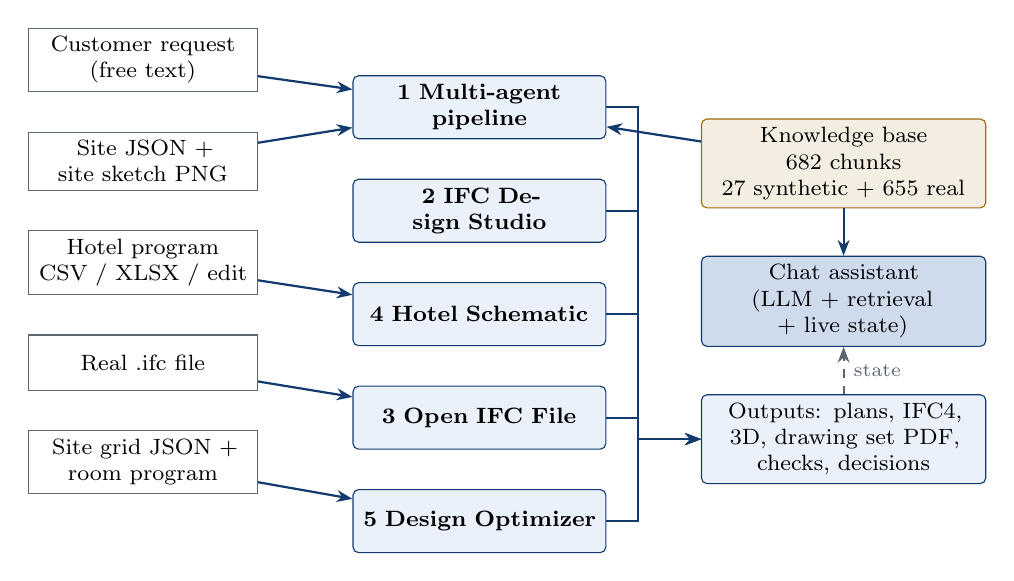
\begin{tikzpicture}[node distance=5mm and 7mm]
\node[data, text width=27mm] (rfp) {Customer request\\(free text)};
\node[data, text width=27mm, below=of rfp] (site) {Site JSON +\\site sketch PNG};
\node[data, text width=27mm, below=of site] (prog) {Hotel program\\CSV / XLSX / edit};
\node[data, text width=27mm, below=of prog] (ifcf) {Real .ifc file};
\node[box, text width=30mm, right=12mm of rfp, yshift=-6mm] (pipe) {\textbf{1 Multi-agent pipeline}};
\node[box, text width=30mm, below=of pipe] (studio) {\textbf{2 IFC Design Studio}};
\node[box, text width=30mm, below=of studio] (hotel) {\textbf{4 Hotel Schematic}};
\node[box, text width=30mm, below=of hotel] (expl) {\textbf{3 Open IFC File}};
\node[data, text width=27mm, below=of ifcf] (grid) {Site grid JSON +\\room program};
\node[box, text width=30mm, below=of expl] (opt) {\textbf{5 Design Optimizer}};
\node[box, fill=amber!12, draw=amber, text width=34mm, right=12mm of studio, yshift=6mm] (kb) {Knowledge base\\682 chunks\\27 synthetic + 655 real};
\node[llm, text width=34mm, below=6mm of kb] (chat) {Chat assistant\\(LLM + retrieval + live state)};
\node[box, text width=34mm, below=6mm of chat] (out) {Outputs: plans, IFC4,\\3D, drawing set PDF,\\checks, decisions};
\draw[arr] (rfp) -- (pipe); \draw[arr] (site) -- (pipe); \draw[arr] (prog) -- (hotel); \draw[arr] (ifcf) -- (expl);
\draw[arr] (kb) -- (pipe); \draw[arr] (kb) -- (chat);
\draw[arr] (pipe.east) -- ++(4mm,0) |- (out.west);
\draw[arr] (studio.east) -- ++(4mm,0) |- (out.west);
\draw[arr] (hotel.east) -- ++(4mm,0) |- (out.west);
\draw[arr] (expl.east) -- ++(4mm,0) |- (out.west);
\draw[arr] (grid) -- (opt); \draw[arr] (opt.east) -- ++(4mm,0) |- (out.west);
\draw[arr, dashed, muted] (out) -- node[lab, right]{state} (chat);
\end{tikzpicture}
\caption{The five modes, the shared knowledge base and the assistant. The layout optimizer (\cref{sec:opt}) runs as its
own mode on the prototype's site grids and as the ``Optimize layouts'' tab of Hotel Schematic.}
\label{fig:arch}
\end{figure}

\begin{table}[H]
\centering\small
\caption{Technology stack.}
\label{tab:stack}
\begin{tabularx}{\linewidth}{@{}l l X@{}}
\toprule
\textbf{Layer} & \textbf{Technology} & \textbf{Used for} \\ \midrule
Language, UI & Python 3.11, Streamlit 1.52 & engines, agents, five-mode app, program editor \\
LLMs & OpenRouter~\citep{openrouter} & light model \code{openai/gpt-oss-20b} (parsing), reasoning model \code{openai/gpt-oss-120b}, arbiter \code{anthropic/claude-sonnet-5}; Chinese-developed models blocked in code; 90\,s timeout \\
Retrieval & Sentence-BERT~\citep{reimers2019sbert}, MiniLM~\citep{wang2020minilm} & 384-d embeddings, cosine search (TF-IDF fallback) \\
State & pydantic & typed blackboard \code{ProjectState} with a full trace \\
Simulation, vision & NumPy~\citep{harris2020numpy}, SciPy~\citep{virtanen2020scipy}, scikit-image~\citep{vanderwalt2014skimage} & rigid-body relaxation; colour masks, connected components \\
BIM & IfcOpenShell~\citep{ifcopenshell} & write IFC4, read and triangulate IFC2X3 \\
Optimization & NumPy, SciPy, \code{concurrent.futures} & decoder, ten-objective fitness, systematic search and memetic GA, parallel plate screening, Pareto/TOPSIS ranking; optimizer report prose by \code{anthropic/claude-sonnet-5.5} (outside the search) \\
Graphics & Plotly~\citep{plotly}, Matplotlib~\citep{hunter2007matplotlib} & interactive 3D and plans; vector drawing sheets \\
Documents & LaTeX (Tectonic), PyMuPDF & report PDFs and merging \\
Verification & pytest, Streamlit AppTest, Playwright & 51 tests; browser run and screenshots \\
\bottomrule
\end{tabularx}
\end{table}

% =====================================================================
\section{The multi-agent pipeline}
\label{sec:pipeline}

\subsection{Blackboard and trace}
All agents read and write one typed object, \code{ProjectState}: the raw inputs, then \code{program}, \code{site},
\code{baap}, \code{conflicts}, the simulation, vision and critic histories, and finally \code{final\_decision}. Every
step runs inside \code{traced\_call}, which records agent, action, model, status, latency and a one-line summary, so
every run can be audited (\cref{fig:snap-trace}).

\subsection{Run order}

\begin{figure}[H]
\centering
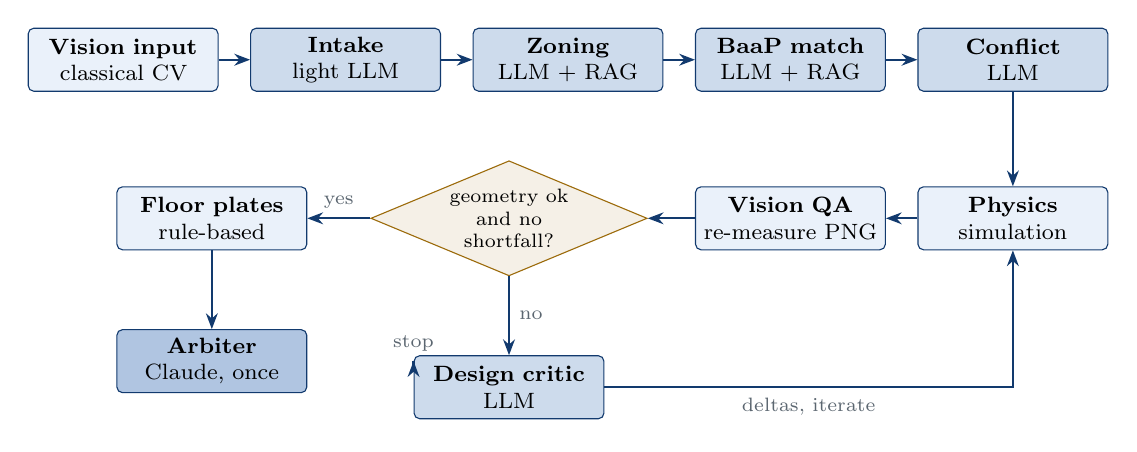
\begin{tikzpicture}[node distance=4mm and 4mm]
\node[box, text width=22mm] (v) {\textbf{Vision input}\\classical CV};
\node[llm, text width=22mm, right=of v] (i) {\textbf{Intake}\\light LLM};
\node[llm, text width=22mm, right=of i] (z) {\textbf{Zoning}\\LLM + RAG};
\node[llm, text width=22mm, right=of z] (b) {\textbf{BaaP match}\\LLM + RAG};
\node[llm, text width=22mm, right=of b] (c) {\textbf{Conflict}\\LLM};
\node[box, text width=22mm, below=12mm of c] (p) {\textbf{Physics}\\simulation};
\node[box, text width=22mm, left=of p] (q) {\textbf{Vision QA}\\re-measure PNG};
\node[dec, left=6mm of q] (g) {geometry ok\\and no\\shortfall?};
\node[llm, text width=22mm, below=10mm of g] (k) {\textbf{Design critic}\\LLM};
\node[box, text width=22mm, left=8mm of g] (f) {\textbf{Floor plates}\\rule-based};
\node[llm, text width=22mm, below=10mm of f, fill=bp!35] (a) {\textbf{Arbiter}\\Claude, once};
\draw[arr] (v) -- (i); \draw[arr] (i) -- (z); \draw[arr] (z) -- (b); \draw[arr] (b) -- (c); \draw[arr] (c) -- (p);
\draw[arr] (p) -- (q); \draw[arr] (q) -- (g);
\draw[arr] (g) -- node[lab, above]{yes} (f);
\draw[arr] (g) -- node[lab, right]{no} (k);
\draw[arr] (k) -| node[lab, pos=0.25, below]{deltas, iterate} (p);
\draw[arr] (k) -- node[lab, above]{stop} (a.east -| k.west) ;
\draw[arr] (f) -- (a);
\end{tikzpicture}
\caption{Pipeline run order. Shaded boxes call an LLM; the others are deterministic. The loop runs at most three
times.}
\label{fig:pipeline}
\end{figure}

\subsection{Agents: inputs, outputs and the division of labour}
The central design rule is that \emph{the model never does arithmetic}: it reads and judges, while Python computes.

\begin{table}[H]
\centering\scriptsize
\caption{What each stage receives, what the LLM does, what Python does, and what is written to the blackboard.}
\label{tab:agents}
\begin{tabularx}{\linewidth}{@{}>{\raggedright\arraybackslash}p{2.5cm} >{\raggedright\arraybackslash}p{2.4cm} >{\raggedright\arraybackslash}X >{\raggedright\arraybackslash}X >{\raggedright\arraybackslash}p{1.9cm}@{}}
\toprule
\textbf{Stage (model)} & \textbf{Input} & \textbf{LLM does} & \textbf{Python does} & \textbf{Output} \\ \midrule
Vision input (none) & sketch PNG + georeference & -- & colour masks, components, pixel$\to$ft, compare with stated lot & \code{cv\_cross\_check} \\
Intake (20b) & request text & extract units, mix, floors, amenities, parking, budget, hard/soft requirements & validate the JSON schema & \code{program} \\
Zoning (20b + RAG) & district, 6 retrieval queries & read code excerpts; return limits or \code{null}, with citations & \textbf{buildable envelope} & \code{site} \\
BaaP (120b + RAG) & program, stacking rules & adjacency plan, utilisation notes & \textbf{module counts, GSF, footprint, cores, accessible units} & \code{baap} \\
Conflict (120b + RAG) & program, site, BaaP, numbers & name conflicts, rate severity, recommend & \textbf{FAR, coverage, stalls, parking area, land left} & \code{conflicts} \\
Physics (none) & envelope, footprint, stalls & -- & rigid-body relaxation & positions, penalty \\
Vision QA (none) & rendered PNG & -- & re-measure footprint, coverage, violations, stall count & \code{cv\_metrics} \\
Critic (120b) & CV metrics, convergence & adjust geometry or stop & clamp to 3 parameters; stop at max iterations & \code{critic} \\
Floor plates (none) & module counts & -- & bay packing, double-loaded corridor & ground + typical floor \\
Arbiter (Claude) & whole blackboard & decision, confidence, narrative, issues, next steps & schema validation & \code{final\_decision} \\
\bottomrule
\end{tabularx}
\end{table}

\subsection{Mathematics computed by the pipeline}

\paragraph{Buildable envelope.} With lot frontage $W_{lot}$ and depth $D_{lot}$, setbacks $s_w, s_e, s_f, s_r$ and a
non-buildable easement of width $e$ on the east side:
\begin{align}
x_{min} &= s_w, & x_{max} &= \min(W_{lot}-s_e,\; W_{lot}-e), & y_{min} &= s_f, & y_{max} &= D_{lot}-s_r,\\
W_{env} &= x_{max}-x_{min}, & D_{env} &= y_{max}-y_{min}, & A_{env} &= W_{env}\,D_{env}.
\end{align}
For Elm Street ($200\times300$\,ft lot, setbacks 10/10/15/20\,ft and a 20\,ft east easement), $W_{env}=180-10=170$\,ft,
$D_{env}=280-15=265$\,ft and $A_{env}=45{,}050$\,SF.

\paragraph{Module counts and areas.} For mix fractions $p_t$ over $T$ unit types and $N$ units, the last type absorbs
rounding:
\begin{equation}
n_t=\operatorname{round}(N p_t)\ \ (t<T),\qquad n_T = N-\sum_{t<T} n_t,
\end{equation}
\begin{equation}
GSF_{u}=\sum_t n_t a_t,\qquad GSF_{b}=\frac{GSF_u}{\phi},\qquad A_{fp}=\frac{GSF_b}{F},\qquad
c=\left\lceil\frac{N/F}{45}\right\rceil ,
\end{equation}
with module areas $a_t$ from the catalogue, grossing factor $\phi=0.85$, $F$ floors and $c$ cores. Elm Street
gives modules $24/54/42$, $GSF_b=111{,}988$\,SF and $A_{fp}=27{,}997$\,SF.

\paragraph{Feasibility.} These numbers are handed to the conflict agent, which is told not to recompute them:
\begin{gather}
GSF_{max}=A_{lot}\cdot FAR,\qquad A_{fp,max}=A_{lot}\,\frac{cov}{100},\qquad S_{req}=\operatorname{round}(r_p N),\qquad A_{park}=330\,S_{req},\\
A_{left}=A_{env}-A_{fp},\qquad \text{surface parking fits}\iff A_{park}\le A_{left}.
\end{gather}
Elm Street: $S_{req}=1.25\times120=150$, so $A_{park}=49{,}500$\,SF, but $A_{left}=17{,}053$\,SF. Surface parking cannot
fit; this is a computed fact that the LLM only names and rates.

\subsection{Decision rules}
The loop exit is code: stop when $\text{geometry\_passed}\wedge \text{shortfall}=0$. Otherwise the critic proposes
deltas to three parameters only, each clamped to $\ge 20$\,ft:
\begin{equation}
w\leftarrow\max(20,\,w+\Delta w),\qquad h\leftarrow\max(20,\,h+\Delta h),\qquad d\leftarrow\max(20,\,d+\Delta d),
\end{equation}
or says to stop. Stopping is forced at the last iteration. The arbiter is instructed not to approve while a critical or
high conflict is unresolved, and is told that \code{geometry\_passed} says nothing about parking.

\subsection{A real run, input to output}

\begin{table}[H]
\centering\small
\caption{Trace of a full run on 2026-10-05 (17:29).}
\label{tab:run}
\begin{tabular}{@{}r l l r l@{}}
\toprule
\# & \textbf{Agent} & \textbf{Model} & \textbf{s} & \textbf{Result} \\ \midrule
1 & vision\_input & classical CV & 0.4 & sketch consistent with site conditions \\
2 & intake & gpt-oss-20b & 14.4 & 120 units, 4 floors \\
3 & zoning & gpt-oss-20b & 9.5 & envelope $170\times265$\,ft (45,050\,SF) \\
4 & baap\_matching & gpt-oss-120b & 20.8 & 120 modules, 111,988\,GSF \\
5 & conflict & gpt-oss-120b & 4.6 & 1 conflict (parking, high); not feasible as requested \\
6 & simulation & physics & 0.0 & 6 steps, penalty 0.438, converged \\
7 & vision\_qa & classical CV & 0.7 & geometry OK; \textbf{stalls 15/150} (shortfall 135); coverage 46.3\% \\
8 & design\_critic & gpt-oss-120b & 4.7 & stop: ``cannot be resolved by geometry tweaks'' \\
9--10 & floor\_plate & rule-based & 1.7 & typical 14 units placed (19 deferred); ground 11 (18 deferred) \\
11 & arbiter & claude-sonnet-5 & 10.4 & \textbf{REVISE} (confidence 0.93) \\
\bottomrule
\end{tabular}
\end{table}

\begin{figure}[H]
\centering
\begin{subfigure}{0.49\linewidth}\includegraphics[width=\linewidth]{\snap{01_pipeline_inputs}}\caption{Input: request and site sketch.}\end{subfigure}\hfill
\begin{subfigure}{0.49\linewidth}\includegraphics[width=\linewidth]{\snap{02_pipeline_running}}\caption{Running: live agent steps.}\end{subfigure}
\caption{Pipeline input and live progress in the app.}
\label{fig:snap-input}
\end{figure}

\begin{figure}[H]
\centering
\begin{subfigure}{0.49\linewidth}\includegraphics[width=\linewidth]{\snap{03_pipeline_overview}}\caption{Output overview: decision, confidence, conflicts.}\end{subfigure}\hfill
\begin{subfigure}{0.49\linewidth}\includegraphics[width=\linewidth]{\snap{04_pipeline_agent_trace}}\caption{Agent trace.}\label{fig:snap-trace}\end{subfigure}
\begin{subfigure}{0.49\linewidth}\includegraphics[width=\linewidth]{\snap{05_pipeline_program_site}}\caption{Intake and zoning outputs.}\end{subfigure}\hfill
\begin{subfigure}{0.49\linewidth}\includegraphics[width=\linewidth]{\snap{06_pipeline_baap_conflicts}}\caption{BaaP modules and conflicts.}\end{subfigure}
\begin{subfigure}{0.49\linewidth}\includegraphics[width=\linewidth]{\snap{07_pipeline_site_simulation}}\caption{Simulation and vision QA.}\end{subfigure}\hfill
\begin{subfigure}{0.49\linewidth}\includegraphics[width=\linewidth]{\snap{09_pipeline_final_decision}}\caption{Arbiter's final decision.}\end{subfigure}
\caption{Pipeline outputs in the app (browser run, 2026-10-05 15:55). The screenshots and \cref{tab:run} come from
different runs with the same inputs; \cref{sec:variability} compares them.}
\label{fig:snap-pipeline}
\end{figure}

\begin{figure}[H]
\centering
\begin{subfigure}{0.30\linewidth}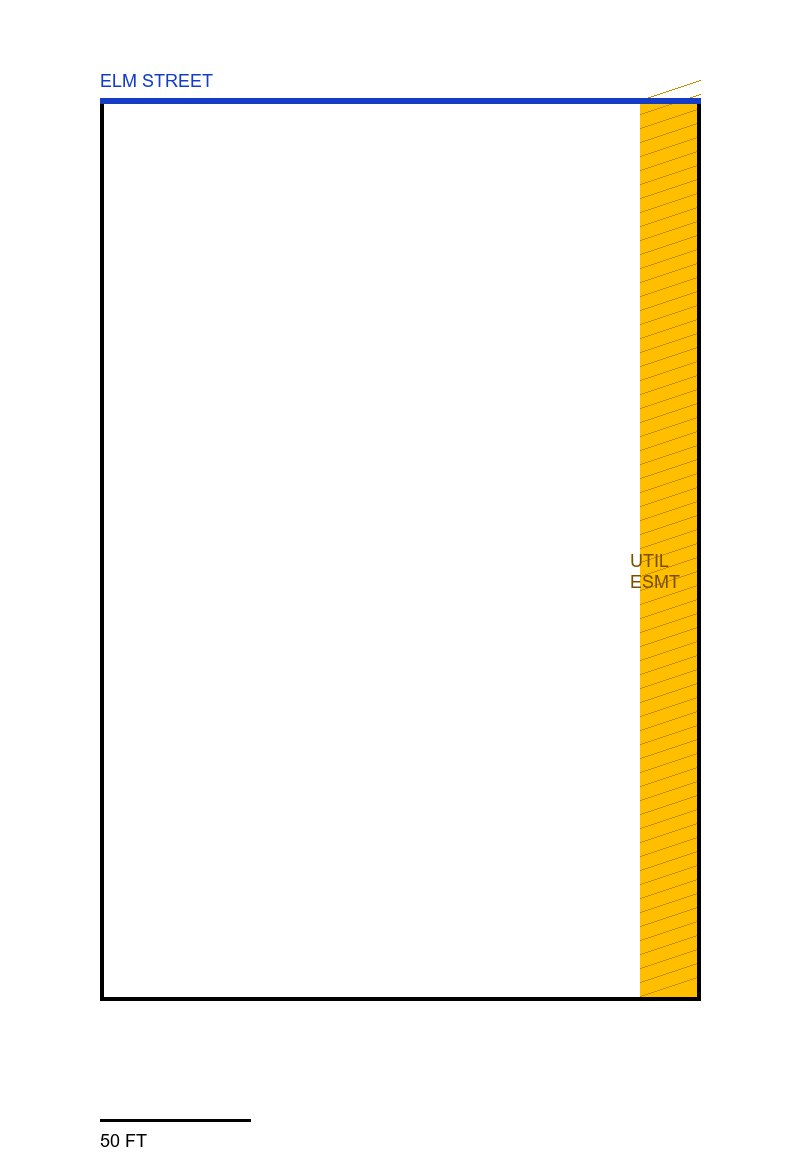
\includegraphics[width=\linewidth]{figures/input_site_sketch.jpg}\caption{Input site sketch.}\end{subfigure}\hfill
\begin{subfigure}{0.30\linewidth}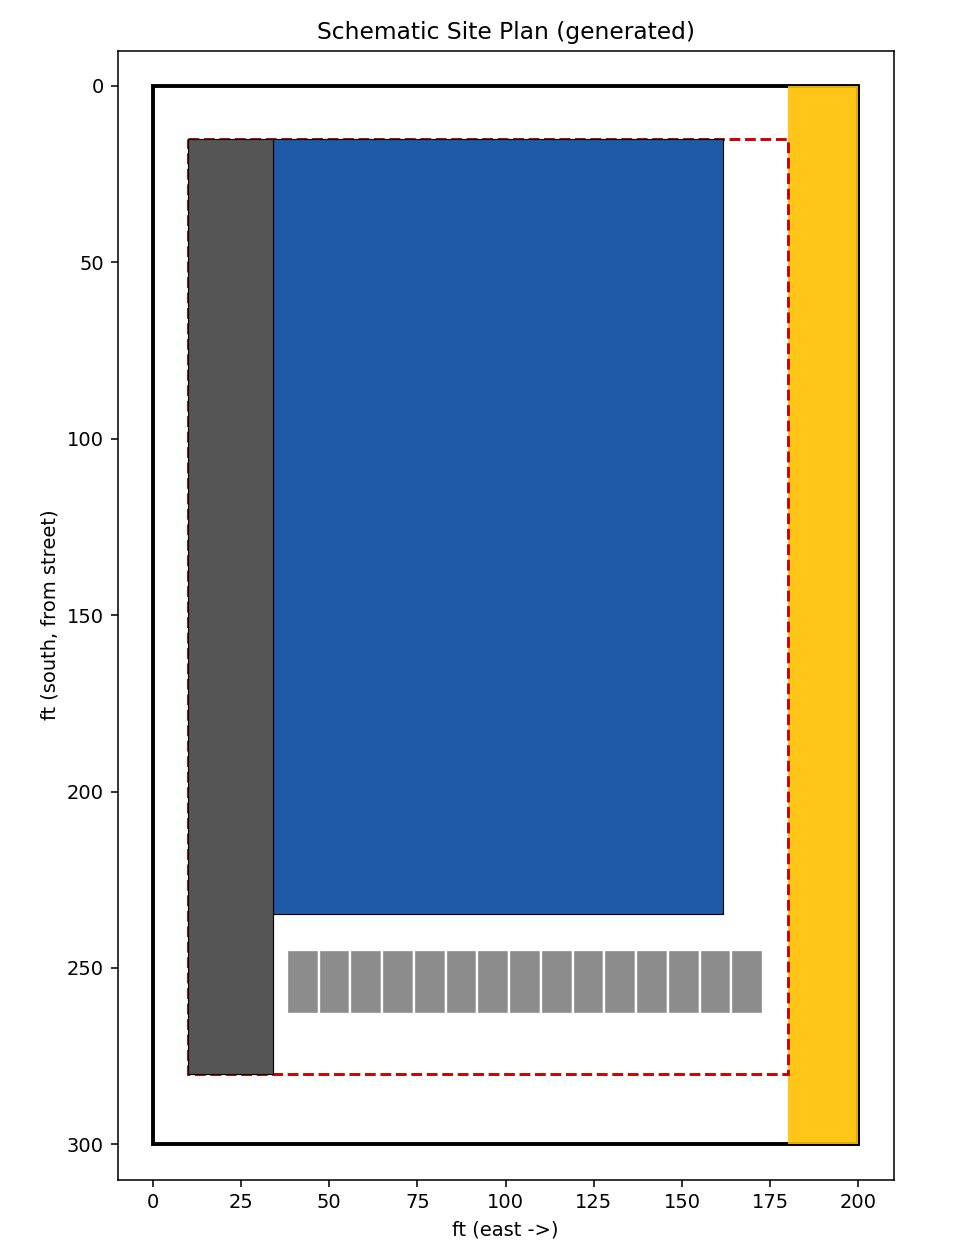
\includegraphics[width=\linewidth]{figures/pipe_site_plan_iter1.jpg}\caption{Simulated site plan.}\end{subfigure}\hfill
\begin{subfigure}{0.36\linewidth}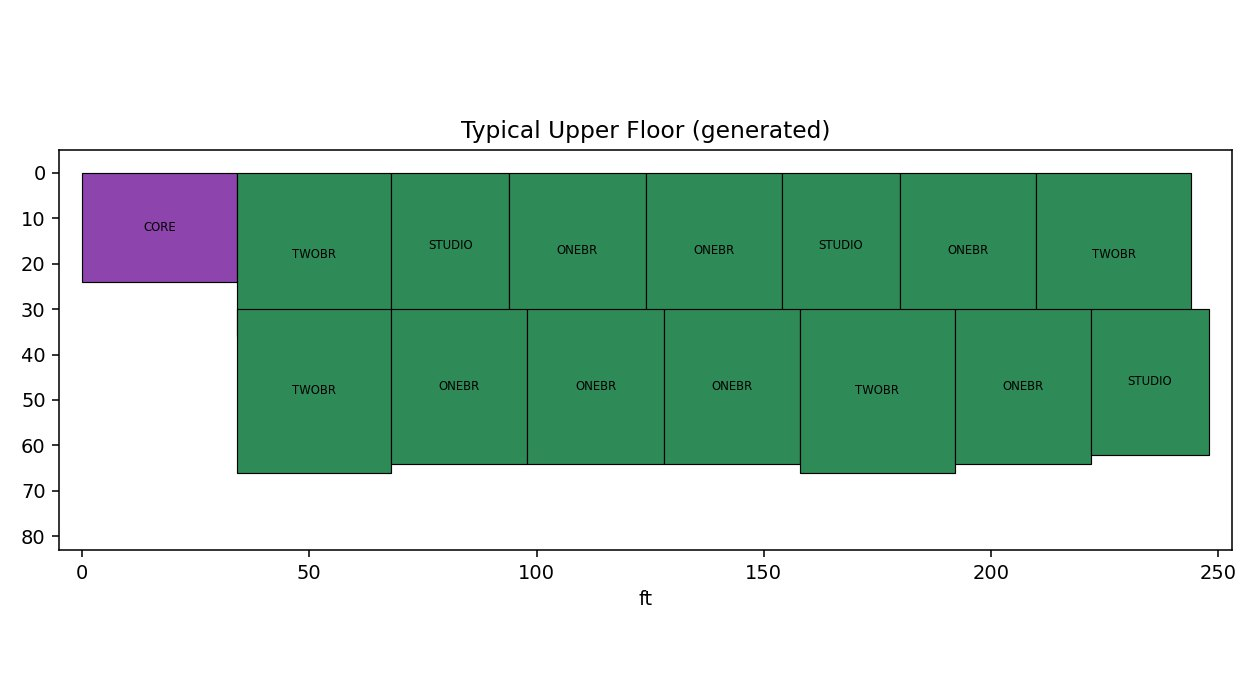
\includegraphics[width=\linewidth]{figures/pipe_floor_plate_typical.jpg}\caption{Typical floor plate.}\end{subfigure}
\caption{Pipeline geometry for the run in \cref{tab:run}: from the sketch to the relaxed site plan (building blue,
driveway grey, one row of 15 stalls, east easement yellow) and the packed floor plate.}
\label{fig:pipe-geom}
\end{figure}

% =====================================================================
\section{Knowledge base and retrieval}
\label{sec:rag}

\begin{table}[H]
\centering\small
\caption{Knowledge-base contents. Every chunk is tagged \code{synthetic} or \code{real}.}
\label{tab:kb}
\begin{tabular}{@{}l l r l@{}}
\toprule
\textbf{Source} & \textbf{Kind} & \textbf{Chunks} & \textbf{Chunking} \\ \midrule
zoning\_code\_sample.md, baap\_catalog.md, baap\_stacking\_rules.md, design\_guidelines.md & synthetic & 27 & heading, then 1,000-char windows \\
RNGD IBC rule CSV & real & 42 & one per rule \\
RNGD IBC workbook & real & 5 & one per sheet \\
2010 ADA Standards PDF & real & 608 & 1,200-char windows per page \\ \midrule
\textbf{Total} & & \textbf{682} & \\
\bottomrule
\end{tabular}
\end{table}

Retrieval-augmented generation~\citep{lewis2020rag} grounds the agents in documents. Chunks $c_i$ and query $q$ are
embedded with MiniLM~\citep{wang2020minilm} through Sentence-BERT~\citep{reimers2019sbert} and normalised, so the score is
the cosine similarity
\begin{equation}
s_i=\mathbf{e}_i^{\top}\mathbf{e}_q=\cos\theta_i,\qquad \lVert\mathbf{e}\rVert_2=1,\qquad
\mathcal{R}_k(q)=\operatorname*{arg\,top\text{-}k}_i\; s_i .
\end{equation}
If the embedding model is unavailable, a TF-IDF backend with
$s_i=\mathbf{t}_i^{\top}\mathbf{t}_q/(\lVert\mathbf{t}_i\rVert\lVert\mathbf{t}_q\rVert)$ is used instead.

\paragraph{Multi-query retrieval.} One broad query on a multi-topic corpus is dominated by the best-matching section.
The zoning agent therefore issues six narrow queries $q_1,\dots,q_6$ and merges their results without duplicates:
\begin{equation}
\mathcal{C}=\bigcup_{j=1}^{6}\mathcal{R}_2(q_j)\quad\text{(deduplicated by source and heading)}.
\end{equation}
This fixed a real failure where setbacks were not retrieved. As an example, the query ``dead-end corridor maximum length
sprinklered'' returns IBC-R1-027 from RNGD's CSV first (score 0.689), the sample code's fire-access section second (0.540)
and IBC-R1-026 third (0.493).

% =====================================================================
\section{Physics engine}
\label{sec:physics}

The site is a 2D rigid-body system. The building ($w\times h$, with $w=\min(0.75\,W_{env},150)$ and $h=A_{fp}/w$) is
movable and starts at the front. The driveway ($24\,\text{ft}\times D_{env}$) and the $9\times18$\,ft stalls are fixed.

\paragraph{Parking capacity is geometry.} With 24\,ft aisles (row pitch 42\,ft):
\begin{equation}
k_{row}=\left\lfloor\frac{W_{env}-24-4}{9}\right\rfloor,\qquad y_0=y_{min}+h+10,\qquad
n_{rows}=\bigl|\{j\in\mathbb{N}: y_0+42j+18\le y_{max}\}\bigr|,\qquad S=\min(S_{req},\,k_{row}\,n_{rows}).
\end{equation}
For Elm Street, $k_{row}=\lfloor142/9\rfloor=15$ and $h=27{,}997/127.5=219.6$\,ft, so $y_0=244.6$ and only $j=0$ fits
($262.6\le280$). That gives one row and $S=15$, exactly the ``15 of 150 stalls'' in \cref{tab:run}.

\paragraph{Forces.} Containment pushes a body back inside the envelope:
\begin{equation}
F^{c}_x=\max(0,x_{min}-x_0)-\max(0,x_1-x_{max}),\qquad F^{c}_y=\max(0,y_{min}-y_0)-\max(0,y_1-y_{max}).
\end{equation}
For overlapping bodies $a,b$ with overlaps
$o_x=\max\bigl(0,\min(a_{x1},b_{x1})-\max(a_{x0},b_{x0})\bigr)$ (and similarly $o_y$), separation acts along the axis
of least overlap, split half to each body:
\begin{equation}
\mathbf{F}^{s}_a=-\mathbf{F}^{s}_b=\tfrac12\begin{cases}(\sigma_x o_x,\,0) & o_x<o_y\\ (0,\,\sigma_y o_y) & \text{otherwise}\end{cases},
\qquad \sigma=\begin{cases}-1 & c_a<c_b\\ +1&\text{otherwise.}\end{cases}
\end{equation}

\paragraph{Integration and convergence.} Semi-implicit Euler with damping $d=0.55$ and gain $g=0.5$:
\begin{equation}
\mathbf{v}_{t+1}=d\,(\mathbf{v}_t+g\,\mathbf{F}_t),\qquad \mathbf{x}_{t+1}=\mathbf{x}_t+\mathbf{v}_{t+1},\qquad
\Pi_t=\sum\lvert F^{c}\rvert+\sum\lvert F^{s}\rvert .
\end{equation}
The run converges when $\Pi_t<0.5$\,ft and stops at 250 steps; positions are then snapped to a 1\,ft grid.

\begin{figure}[H]
\centering
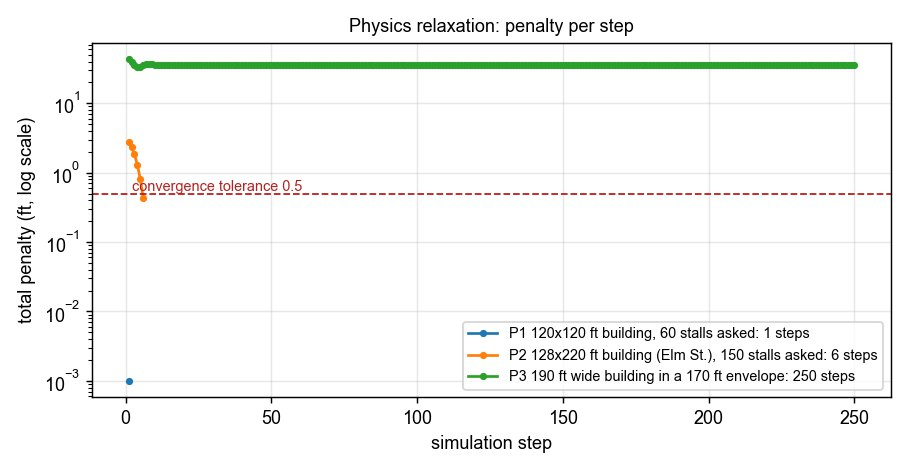
\includegraphics[width=0.78\linewidth]{figures/fig_physics_convergence.jpg}
\caption{Penalty per step in three experiments.
P1: a building that already fits converges in one step.
P2: the Elm Street building converges in six steps.
P3: a 190\,ft-wide building in a 170\,ft envelope can never satisfy containment, so the penalty plateaus at 36\,ft.
P3 is the case the critic must report as a program/site conflict.}
\label{fig:physics}
\end{figure}

The engine does not change the number of stalls, because the rows are fixed at set-up. The preference for the
building at the front is set by the initial placement; no attraction force is applied.

% =====================================================================
\section{Computer-vision QA and the critic}
\label{sec:cv}

The QA agent re-measures the \emph{rendered} PNG rather than trusting the simulation. The design decision (kept from the
project's start) is classical CV, not a vision LLM: measuring a setback or counting stalls is a precise geometric
question.
\begin{enumerate}
\item \textbf{Calibration.} From two reference points written by the renderer,
$x_{ft}=x^0_{ft}+(x_{px}-x^0_{px})\,s_x$ with $s_x=\dfrac{x^1_{ft}-x^0_{ft}}{x^1_{px}-x^0_{px}}$ (same for $y$).
\item \textbf{Colour masks.} A pixel belongs to class $k$ if $\sum_{c\in\{R,G,B\}}\lvert I_c-\mathrm{ref}^k_c\rvert\le30$.
\item \textbf{Building.} The mask's bounding box gives $A_{fp}$; coverage is $100A_{fp}/A_{lot}$; a setback violation is
recorded when the box is outside the envelope by more than 1\,ft.
\item \textbf{Stalls.} Connected components of the parking mask, keeping components larger than 15\% of the largest:
$S_{det}=\lvert\{k: |C_k|>0.15\max_j|C_j|\}\rvert$, and shortfall $=\max(0,S_{req}-S_{det})$.
\end{enumerate}
\code{geometry\_passed} and \code{parking\_shortfall} are separate fields, so a design can be geometrically clean and
still fail on parking.

% =====================================================================
\section{IFC Design Studio}
\label{sec:ifc}

A deterministic generator produces a building from a parameter vector $\mathbf{p}$ (lot, easement, zoning preset, units
and mix, floors, wings, parking type, corridor width, floor heights):
\begin{enumerate}
\item \textbf{Modules.} The mix is turned into module counts from the shared catalogue, including accessible units,
core, lobby, fitness and BOH.
\item \textbf{Layout and selection.} Units are placed on double-loaded wings inside the setbacks and easement. The
generator tries 1--3 wings and keeps the layout that scores best on: all units placed, inside the envelope, fire lane
present, fewest wings.
\item \textbf{Parking.} Surface stalls come from a scan of free land; the podium option adds stalls under the building.
\item \textbf{Checks.} Ten sample-zoning checks, plus the measurable subset of RNGD's IBC rules (height, stories, exit
travel, dead-end corridor, exits per story).
\item \textbf{IFC4 output.} IfcOpenShell writes project, site, building and one storey per level, with the volumes and
slabs on each storey; the 3D view re-reads the file.
\end{enumerate}

\begin{table}[H]
\centering\small
\caption{The five scenarios (computed).}
\label{tab:ifc}
\begin{tabular}{@{}l c c c c c l l@{}}
\toprule
\textbf{Scenario} & \textbf{Units} & \textbf{Stories} & \textbf{FAR} & \textbf{Cover.} & \textbf{Parking} & \textbf{Sample zoning} & \textbf{Real IBC fails} \\ \midrule
Baseline, 4 floors, surface & 120/120 & 4 & 3.16 & 79.1\% & 23/150 & \FAIL\ (4) & R1-027 \\
Right-sized, 60 units, podium & 60/60 & 5 & 2.31 & 46.3\% & 75/75 & \PASS & R1-027 \\
Podium, 5 floors & 120/120 & 6 & 3.74 & 62.4\% & 120/150 & \FAIL\ (7) & R1-007, 008, 027 \\
Dense R-6, 7 floors & 120/120 & 8 & 4.01 & 50.2\% & 90/90 & \FAIL\ (3) & R1-005--008, 027 \\
Suburban R-2, 3 floors & 60/60 & 3 & 1.62 & 54.1\% & 10/120 & \FAIL\ (3) & R1-027 \\
\bottomrule
\end{tabular}
\end{table}

A real finding follows from the cross-check: even the scenario that passes all sample-zoning checks fails RNGD's
50\,ft dead-end corridor rule (IBC-R1-027), because a single core leaves a long dead end.

\begin{figure}[H]
\centering
\begin{subfigure}{0.49\linewidth}\includegraphics[width=\linewidth]{\snap{10_ifc_baseline_3d_model}}\caption{Baseline IFC4 model in 3D.}\end{subfigure}\hfill
\begin{subfigure}{0.49\linewidth}\includegraphics[width=\linewidth]{\snap{11_ifc_baseline_site_plan}}\caption{Baseline site plan.}\end{subfigure}
\begin{subfigure}{0.49\linewidth}\includegraphics[width=\linewidth]{\snap{12_ifc_baseline_compliance}}\caption{Baseline: sample-zoning checks.}\end{subfigure}\hfill
\begin{subfigure}{0.49\linewidth}\includegraphics[width=\linewidth]{\snap{13_ifc_baseline_real_ibc_check}}\caption{Baseline: RNGD's real IBC rules.}\end{subfigure}
\begin{subfigure}{0.49\linewidth}\includegraphics[width=\linewidth]{\snap{15_ifc_rightsized_compliance}}\caption{Right-sized: all sample checks pass.}\end{subfigure}\hfill
\begin{subfigure}{0.49\linewidth}\includegraphics[width=\linewidth]{\snap{16_ifc_rightsized_3d}}\caption{Right-sized model in 3D.}\end{subfigure}
\caption{IFC Design Studio: input scenario to output model and checks.}
\label{fig:snap-ifc}
\end{figure}

% =====================================================================
\section{Viewing a real IFC model}
\label{sec:explorer}

IfcOpenShell reads the file's header, spatial structure and element counts, and its geometry iterator triangulates
every element. Meshes are merged per IFC class with NumPy and cached. Real files often contain stray elements far from
the building, which shrink the view to a dot. The model is therefore recentred on the median of its structural
elements, and outliers are excluded from the view (never from the file):
\begin{equation}
\mathbf{o}=\operatorname{median}\{\mathbf{c}_e: e\in\text{structural}\},\qquad
\text{exclude } e \iff \lVert\mathbf{c}_e-\mathbf{o}\rVert>\max(4\,\delta,\,50\,\text{m}),
\end{equation}
with $\delta$ the building diagonal.

\begin{table}[H]
\centering\small
\caption{The real model (CDI Solutions, Metairie Bank).}
\begin{tabular}{@{}l l@{}}
\toprule
Schema / project & IFC2X3 / METAIRIE BANK \\
Storeys & FIRST FLOOR (0.0\,m), MIDDLE ROOF (14.0\,m), HIGH ROOF (16.0\,m) \\
Elements / meshes & 1,537 IfcElements / 881 triangulated meshes \\
Largest classes & IfcMember 467, IfcBuildingElementProxy 166, IfcPlate 148, IfcWall 144, IfcWallStandardCase 139 \\
Building diagonal & 134.8\,m \\
Excluded outliers & 4 ``Night DropBox'' items at 896.5\,m \\
\bottomrule
\end{tabular}
\end{table}

\begin{figure}[H]
\centering
\begin{subfigure}{0.49\linewidth}\includegraphics[width=\linewidth]{\snap{17_explorer_3d_model}}\caption{Recentred 3D view.}\end{subfigure}\hfill
\begin{subfigure}{0.49\linewidth}\includegraphics[width=\linewidth]{\snap{18_explorer_summary}}\caption{Model summary.}\end{subfigure}
\caption{Opening a real IFC file.}
\end{figure}

% =====================================================================
\section{Hotel schematic generation}
\label{sec:hotel}

The hotel mode uses \emph{no language model} to create the design. It is a deterministic function
\begin{equation}
\mathcal{D}:\ (\text{program},\ \text{envelope},\ F,\ h_1,\ h_t)\ \longmapsto\ (\text{levels, rooms, checks, drawings}),
\end{equation}
where $F$ is the number of guest floors and $h_1, h_t$ are the floor-to-floor heights.

\subsection{Program}
The default program is RNGD's Living\,+\,Lodging space allocation~\citep{rngd2025ll}, row for row: 117 keys in nine
types and 59,350\,SF net. Rows are \emph{(name, count, total area, category)}. Programs can also be uploaded as CSV/XLSX
or edited in the app (\cref{fig:snap-hotel-a}). Rows are routed as follows:
\begin{itemize}
\item guest rows become keys, each with area (row total)/(count);
\item small repeated rooms (count $\ge2$, under 150\,SF each: Ice, IT, Jan, Supplies) are placed once on every guest floor;
\item small single BOH rooms go to the Level~1 core zone;
\item tenant space becomes the retail block;
\item stairs and corridors are generated, not packed;
\item every other row goes to the Level~1 bands.
\end{itemize}

\subsection{Guest floors}

\begin{figure}[H]
\centering
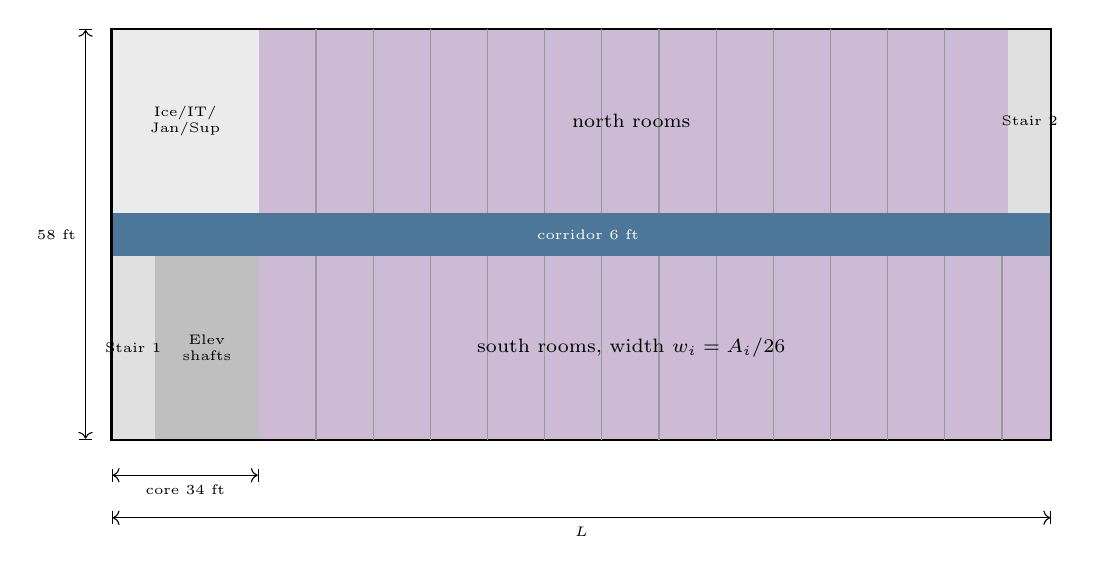
\begin{tikzpicture}[x=0.55mm,y=0.9mm]
\fill[guest] (34,0) rectangle (217,26); \fill[guest] (34,32) rectangle (207,58);
\fill[shared] (0,26) rectangle (217,32);
\fill[black!12] (0,0) rectangle (10,26); \fill[black!12] (207,32) rectangle (217,58);
\fill[black!25] (10,0) rectangle (34,26); \fill[black!8] (0,32) rectangle (34,58);
\draw[thick] (0,0) rectangle (217,58);
\foreach \x in {47.2,60.4,73.6,86.8,100,113.2,126.4,139.6,152.8,166,179.2,192.4,205.6} \draw[black!40] (\x,0)--(\x,26);
\foreach \x in {47.2,60.4,73.6,86.8,100,113.2,126.4,139.6,152.8,166,179.2,192.4} \draw[black!40] (\x,32)--(\x,58);
\node[font=\tiny] at (5,13) {Stair 1}; \node[font=\tiny, align=center] at (22,13) {Elev\\shafts};
\node[font=\tiny, align=center] at (17,45) {Ice/IT/\\Jan/Sup};
\node[font=\tiny] at (212,45) {Stair 2};
\node[font=\tiny, white] at (110,29) {corridor 6 ft};
\node[font=\scriptsize] at (120,13) {south rooms, width $w_i=A_i/26$};
\node[font=\scriptsize] at (120,45) {north rooms};
\draw[|<->|] (0,-5)--(34,-5) node[midway,below,font=\tiny]{core 34 ft};
\draw[|<->|] (0,-11)--(217,-11) node[midway,below,font=\tiny]{$L$};
\draw[|<->|] (-6,0)--(-6,58) node[midway,left,font=\tiny]{58 ft};
\end{tikzpicture}
\caption{A guest floor: double-loaded corridor, west core (Stair 1, two elevators, shafts), per-floor support rooms,
and Stair 2 at the east end, so the corridor has an exit at each end.}
\label{fig:wing}
\end{figure}

\paragraph{Room size.} With room depth $d=26$\,ft, $w_i=A_i/26$; a King is $343/26=13.2$\,ft wide.

\paragraph{Keys to floors and sides.} Keys are sorted by area (largest first) and assigned round-robin, so suites
spread over the floors. On each floor, rooms are balanced greedily between the south and north sides; the north side
starts 10\,ft behind because of Stair 2.

\begin{algorithm}[H]
\caption{Guest-floor layout}
\label{alg:wing}
\begin{algorithmic}[1]
\Require keys $k_0,\dots,k_{N-1}$ sorted by area (descending), guest floors $F$
\For{$k = 0$ \textbf{to} $N-1$} \State floor$(k) \gets k \bmod F$ \EndFor
\For{each floor $f$}
  \State $R_S \gets 0,\ R_N \gets 10$ \Comment{Stair 2 occupies the north end}
  \For{each key $i$ on floor $f$}
    \State $s^\ast \gets \arg\min_{s\in\{S,N\}} R_s$;\quad place $i$ at $x=34+R_{s^\ast}$ on side $s^\ast$;\quad $R_{s^\ast}\gets R_{s^\ast}+A_i/26$
  \EndFor
\EndFor
\State $L \gets 34+\max_f \max(R_S, R_N)$ \Comment{all guest floors share the longest wing}
\end{algorithmic}
\end{algorithm}

\paragraph{Massing.}
\begin{equation}
G_{level}=58\,L,\qquad H=h_1+F\,h_t,\qquad h_1=16\ \text{ft},\ h_t=10.75\ \text{ft (from the L+L elevations).}
\end{equation}
Default program: $L=217$\,ft and $H=16+5(10.75)=69.75$\,ft.

\paragraph{Level 1.} The core is stacked under the tower. The lobby goes first on the street band; the remaining rooms
are sorted by size and go to the shorter band. The retail block is full depth at the east end and wraps Stair~2, with
length $\ell=(A_{ten}+A_{stair})/58$. Default: bands end at 168.7\,ft and retail adds 65.4\,ft, so Level~1 is
234\,ft long, inside the 265\,ft envelope.

\subsection{Code and ADA screen}
\begin{table}[H]
\centering\small
\caption{Hotel code screen: formulas and default results. Rules come from RNGD's CSV~\citep{rngd2026ibc}; ADA tables
from~\citep{doj2010ada}.}
\label{tab:hotelcode}
\begin{tabularx}{\linewidth}{@{}l X l@{}}
\toprule
\textbf{Rule} & \textbf{Test} & \textbf{Default} \\ \midrule
IBC-R1-007 stories & $F+1\le5$ (Level 1 is a story above grade plane) & 6: \FAIL \\
IBC-R1-005 height & $H\le85$\,ft & 69.75: \PASS \\
IBC-R1-010 area per story & $\max G_{level}\le72{,}000$\,SF & 13,575: \PASS \\
IBC-R1-012 high-rise screen & $h_1+(F-1)h_t\le75$\,ft & 59.0: \PASS \\
IBC-R1-015 exits & 2 stairs and $OL_{level}\le500$ & 316: \PASS \\
IBC-R1-018 exit separation & $L-10\ge\frac13\sqrt{L^2+58^2}$ & $207\ge75$: \PASS \\
IBC-R1-023 travel & $T=\frac{L-10}{2}+26\le250$\,ft & 129.5: \PASS \\
IBC-R1-025 corridor & $72\ge44$\,in & \PASS \\
IBC-R1-027 dead end & $\max(5,\ L-(L-5))=5\le50$\,ft & \PASS \\
IBC-R1-028 door & $34\ge32$\,in clear & \PASS \\
ADA 224.2 & Table 224.2: 101--150 rooms need $5+2$ (roll-in) $=7$ & 7: \PASS \\
ADA 224.4 & Table 224.4: 101--150 rooms need 12 communication rooms & not designated: \REVIEW \\
ADA 224.5 & accessible rooms dispersed over room types & 3 types: \PASS \\
\bottomrule
\end{tabularx}
\end{table}

Occupant load uses the CSV's IBC Table 1004.5 factors $f_r$ (residential 200, business 150, storage 300, mercantile 60,
exercise 50, kitchen 200, lobby 15 net):
\begin{equation}
OL_{level}=\sum_{r\in\text{level}}\left\lceil\frac{A_r}{f_r}\right\rceil .
\end{equation}
Gross area is reported three ways. The source sheets give 74,195\,SF and the drawn total is 76,508\,SF. The meeting rule
gives
\begin{equation}
G_{rule}=100\left\lceil\frac{N_{net}(1+c)(1+w_b)}{100}\right\rceil=100\left\lceil\frac{59{,}350\times1.33\times1.08}{100}\right\rceil=85{,}300\ \text{SF}.
\end{equation}

\subsection{From numbers to drawings}
Each room type is defined once in local coordinates $(u,v)$: $u$ along the corridor, $v$ from the corridor ($v=0$) to
the window ($v=26$). The definition includes walls with openings, door swings, bathroom fixtures, beds by type, closet,
suite partition, spa tub and ADA turning circles (\cref{fig:unit}). A south-side room at $(x_r,y_r)$ of width $w$ is
placed by
\begin{equation}
(x,y)=\bigl(x_r+(w-u\ \text{if mirrored else}\ u),\ \ y_r+26-v\bigr),
\end{equation}
with alternate rooms mirrored so bathrooms pair up (north side: $y=y_r+v$).

For the 3D views, the same primitives are extruded to boxes and drawn by an orthographic projector. With camera
azimuth $\theta$ and elevation $\varphi$:
\begin{equation}
\mathbf{c}=(\cos\varphi\cos\theta,\ \cos\varphi\sin\theta,\ \sin\varphi),\quad
\mathbf{r}=(-\sin\theta,\cos\theta,0),\quad \mathbf{u}=\mathbf{c}\times\mathbf{r},\quad (X,Y)=(\mathbf{p}\!\cdot\!\mathbf{r},\ \mathbf{p}\!\cdot\!\mathbf{u}).
\end{equation}
A face with normal $\mathbf{n}$ is drawn only if $\mathbf{n}\cdot\mathbf{c}>0$. Faces are drawn far to near by depth
$\mathbf{p}\cdot\mathbf{c}$, the painter's algorithm~\citep{newell1972painter}. Walls on the camera side are drawn last
so they correctly hide the interior.

\begin{figure}[H]
\centering
\begin{subfigure}{0.26\linewidth}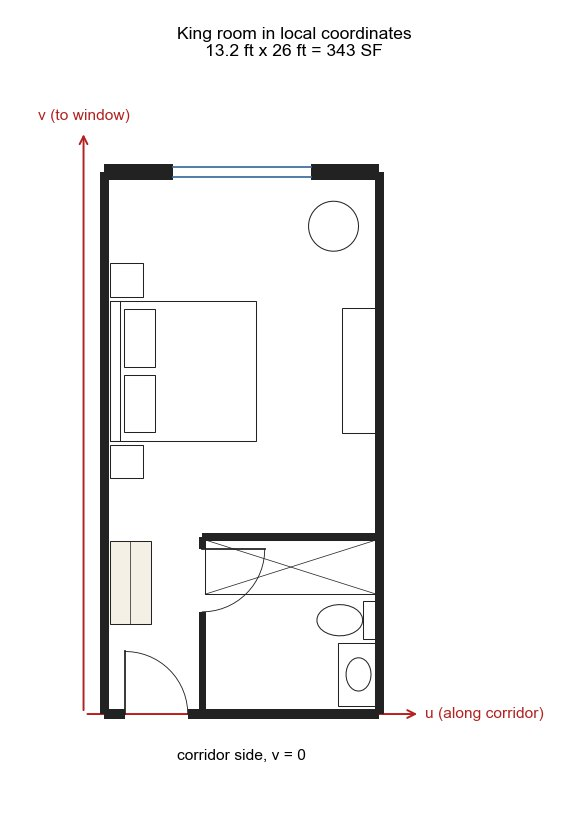
\includegraphics[width=\linewidth]{figures/fig_unit_local_coords.jpg}\caption{King in $(u,v)$.}\label{fig:unit}\end{subfigure}\hfill
\begin{subfigure}{0.70\linewidth}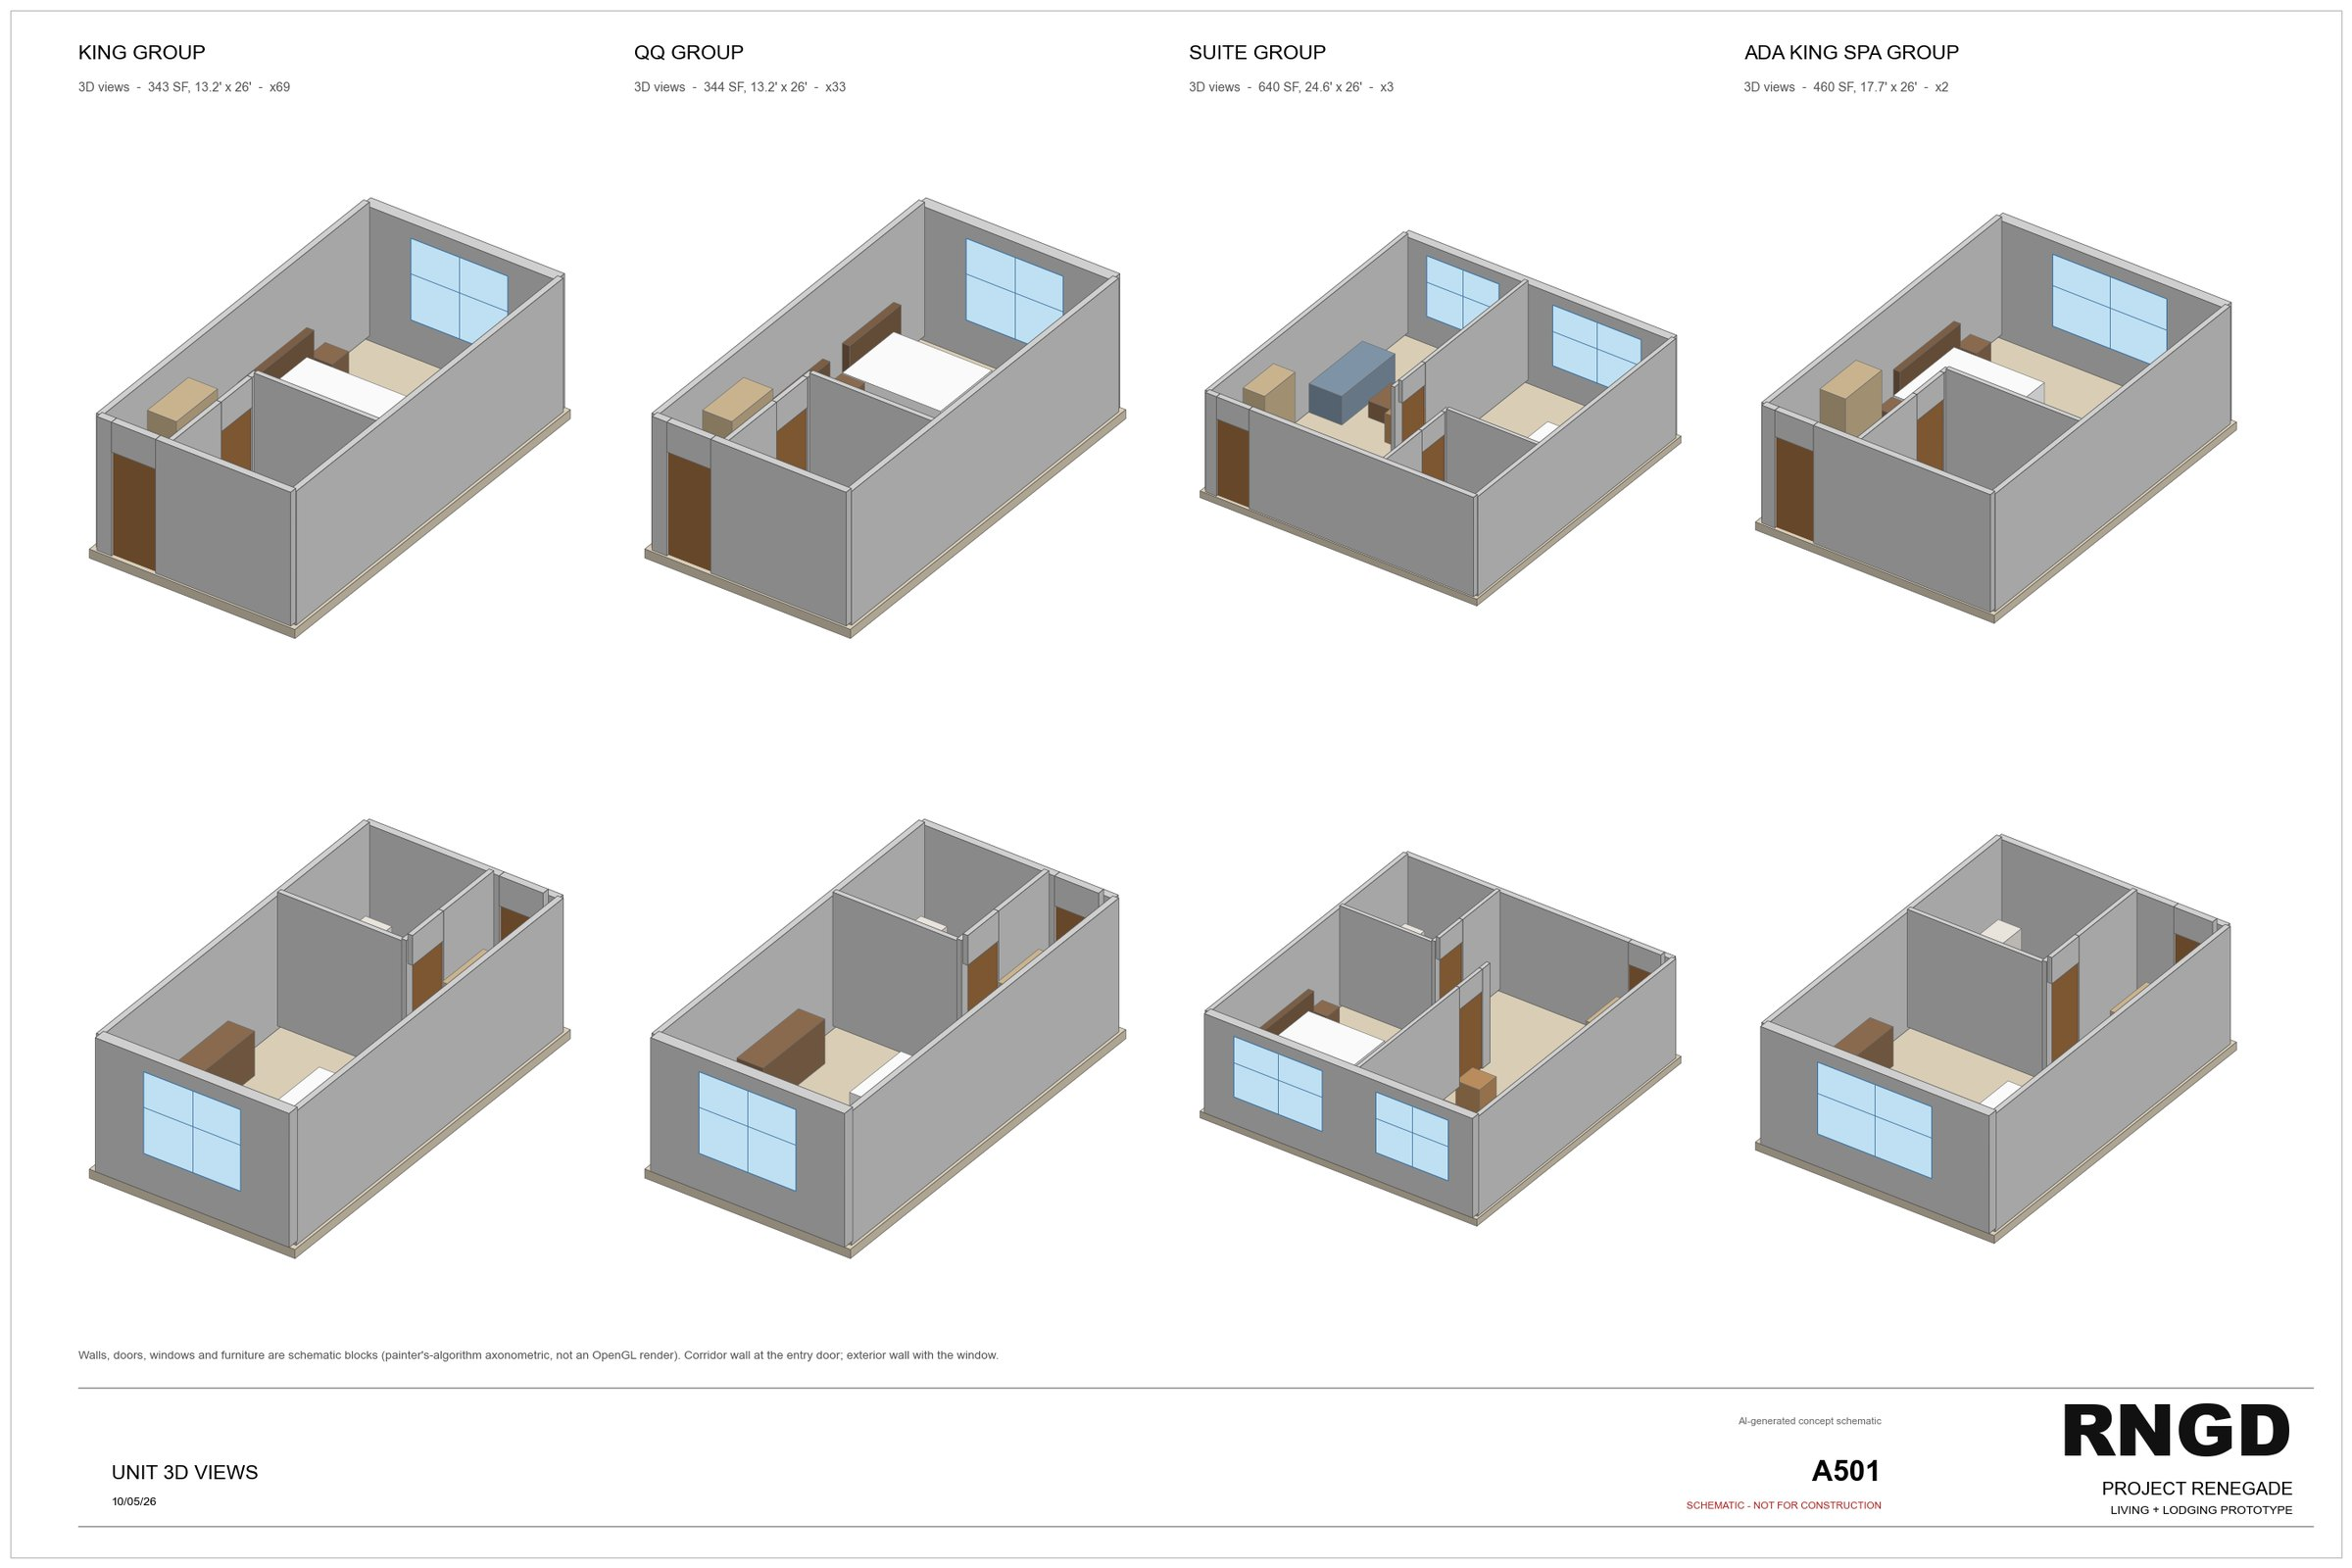
\includegraphics[width=\linewidth]{figures/sheet_A501.jpg}\caption{Sheet A501: unit 3D views.}\end{subfigure}
\caption{One local definition per room type drives every plan and every 3D view.}
\end{figure}

\subsection{The app: inputs, outputs and interaction}
\begin{figure}[H]
\centering
\begin{subfigure}{0.49\linewidth}\includegraphics[width=\linewidth]{\snap{21_hotel_program}}\caption{Input: editable program.}\end{subfigure}\hfill
\begin{subfigure}{0.49\linewidth}\includegraphics[width=\linewidth]{\snap{23_hotel_program_detail}}\caption{Detailed program.}\end{subfigure}
\begin{subfigure}{0.49\linewidth}\includegraphics[width=\linewidth]{\snap{20_hotel_overview}}\caption{Output: KPIs, room-by-room 3D, fixes.}\end{subfigure}\hfill
\begin{subfigure}{0.49\linewidth}\includegraphics[width=\linewidth]{\snap{24_hotel_plan_level2}}\caption{Interactive Level 2 plan.}\end{subfigure}
\caption{Hotel Schematic mode (1): program in, design out.}
\label{fig:snap-hotel-a}
\end{figure}

\begin{figure}[H]
\centering
\begin{subfigure}{0.49\linewidth}\includegraphics[width=\linewidth]{\snap{26_hotel_room}}\caption{Room mix by floor.}\end{subfigure}\hfill
\begin{subfigure}{0.49\linewidth}\includegraphics[width=\linewidth]{\snap{27_hotel_unit}}\caption{Unit type: plan and 3D.}\end{subfigure}
\begin{subfigure}{0.49\linewidth}\includegraphics[width=\linewidth]{\snap{28_hotel_code}}\caption{Code and ADA screen.}\end{subfigure}\hfill
\begin{subfigure}{0.49\linewidth}\includegraphics[width=\linewidth]{\snap{29_hotel_report_results}}\caption{Generated report and its results.}\end{subfigure}
\caption{Hotel Schematic mode (2): mix, units, code screen and report.}
\end{figure}

\subsection{The drawing set}
\begin{figure}[H]
\centering
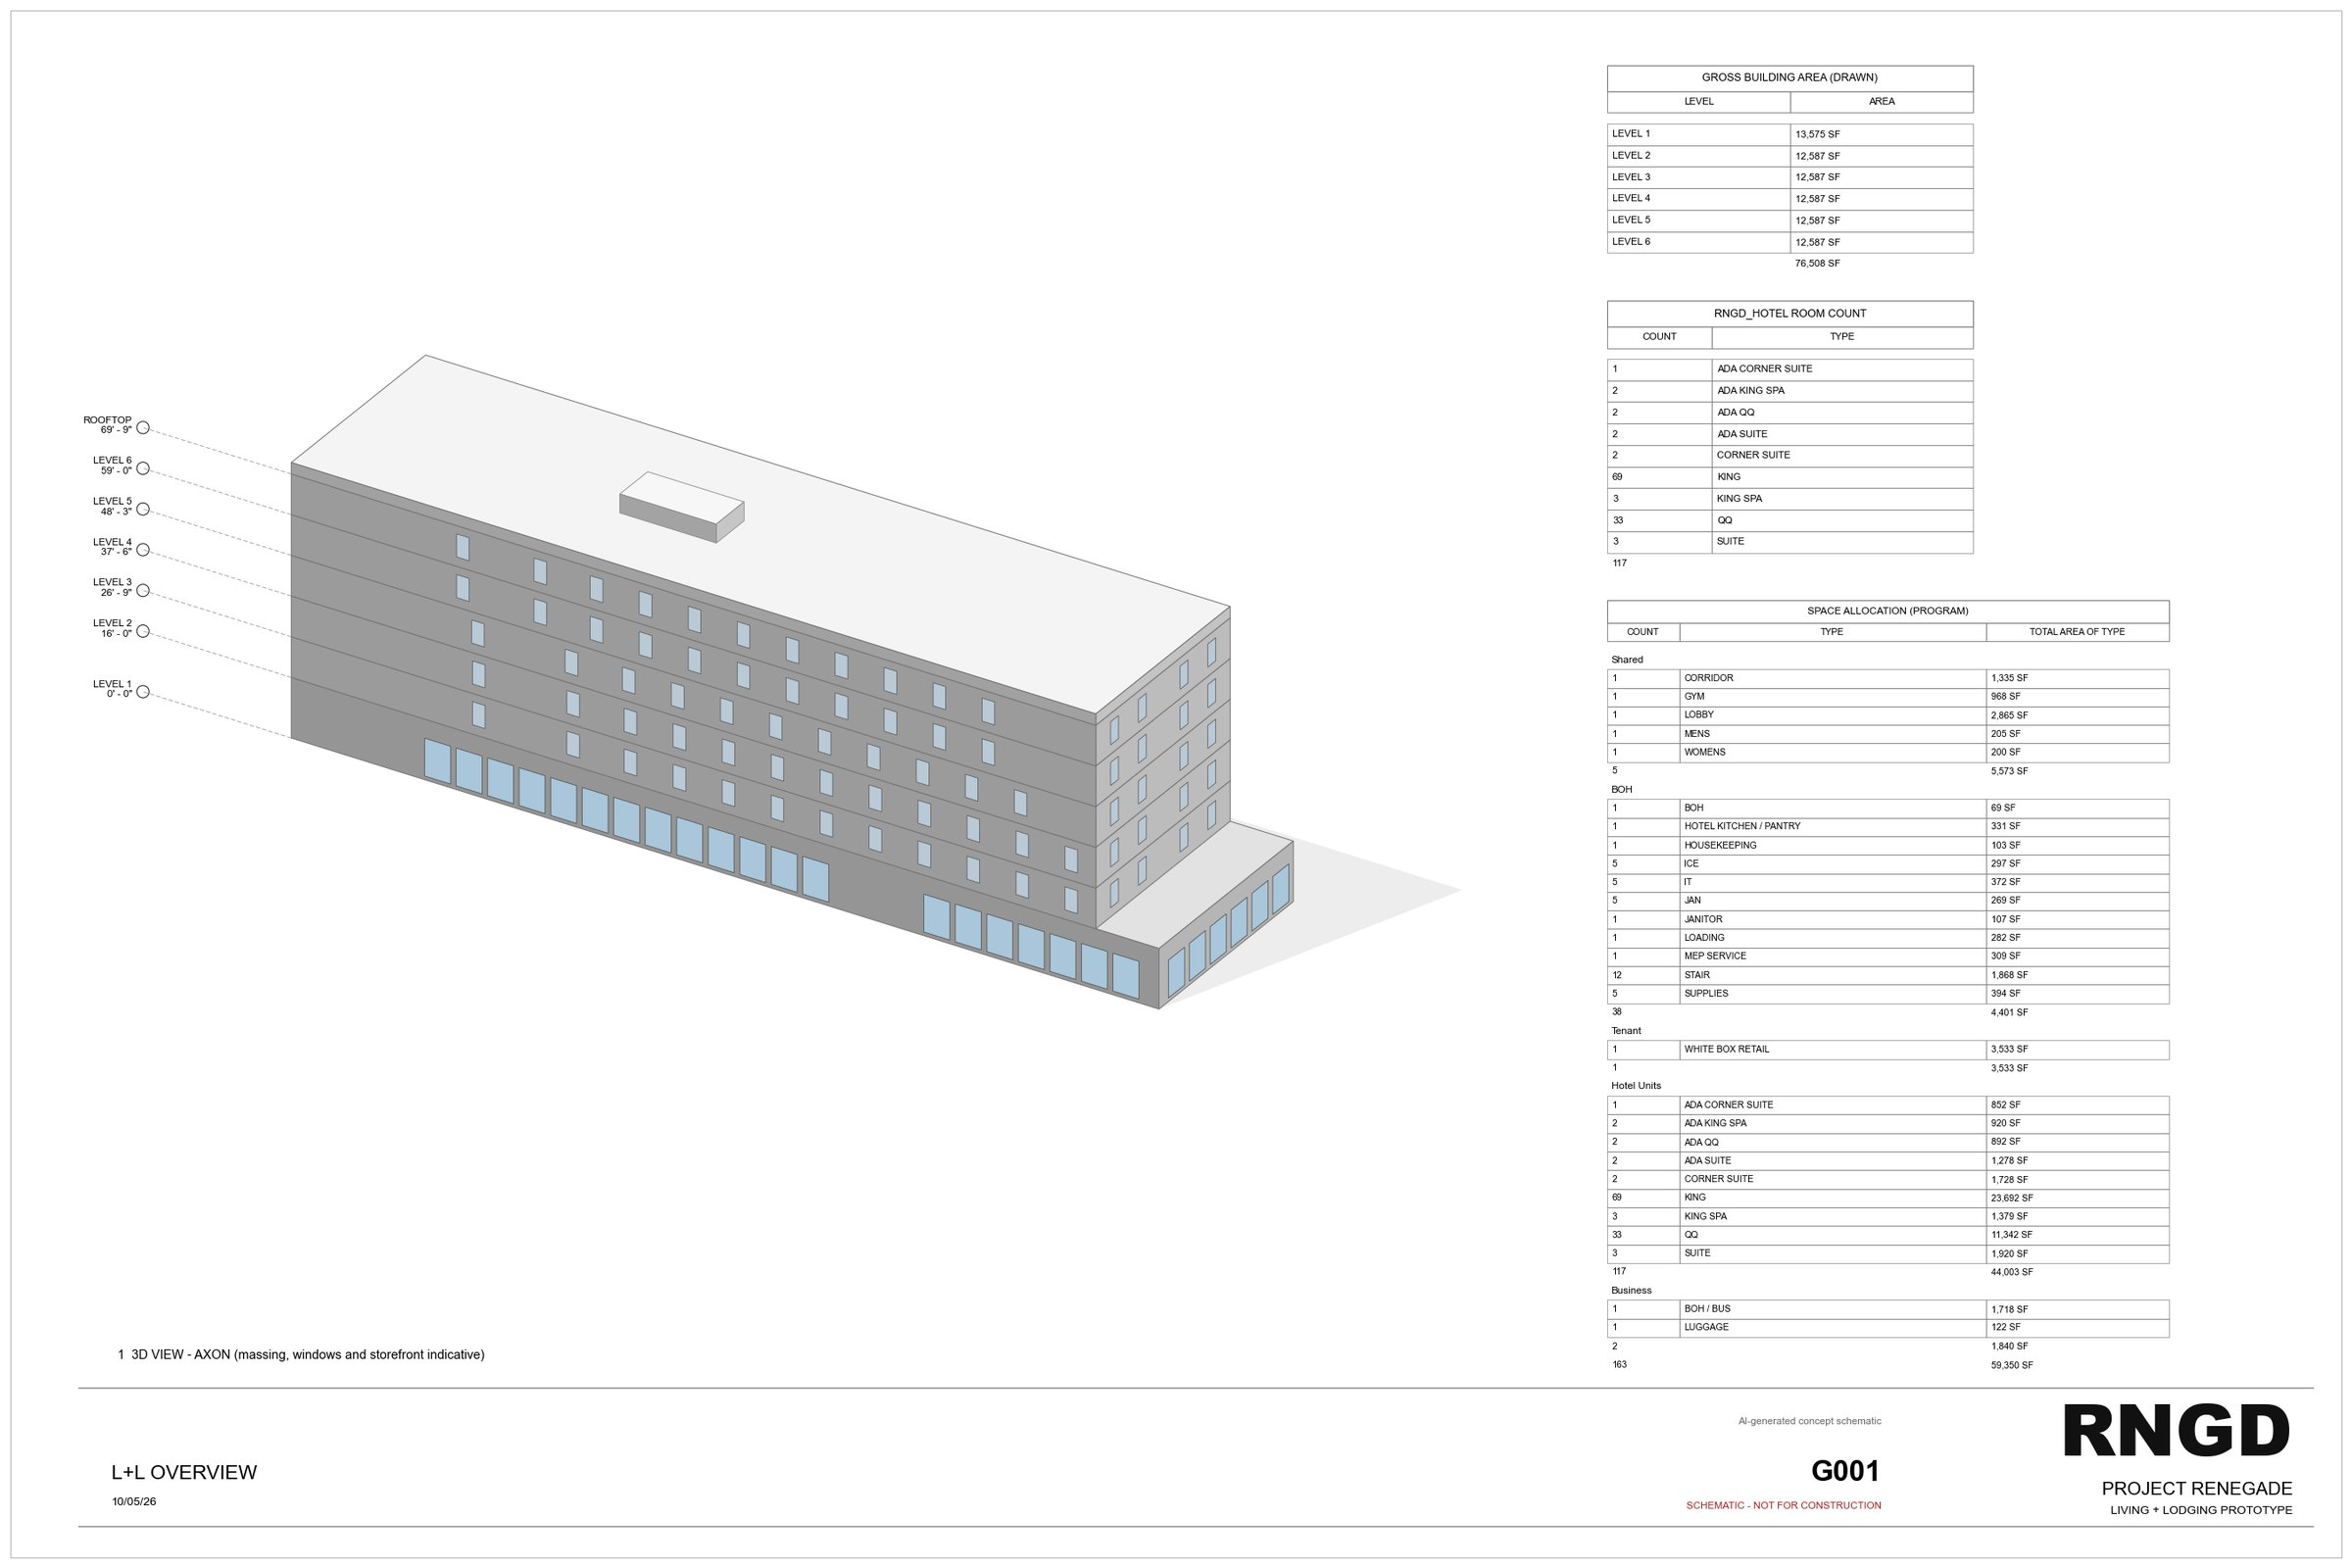
\includegraphics[width=\linewidth]{figures/sheet_G001.jpg}
\caption{Sheet G001 in RNGD's L+L format: axonometric with level markers and the gross area, room count and space
allocation schedules.}
\end{figure}
\begin{figure}[H]
\centering
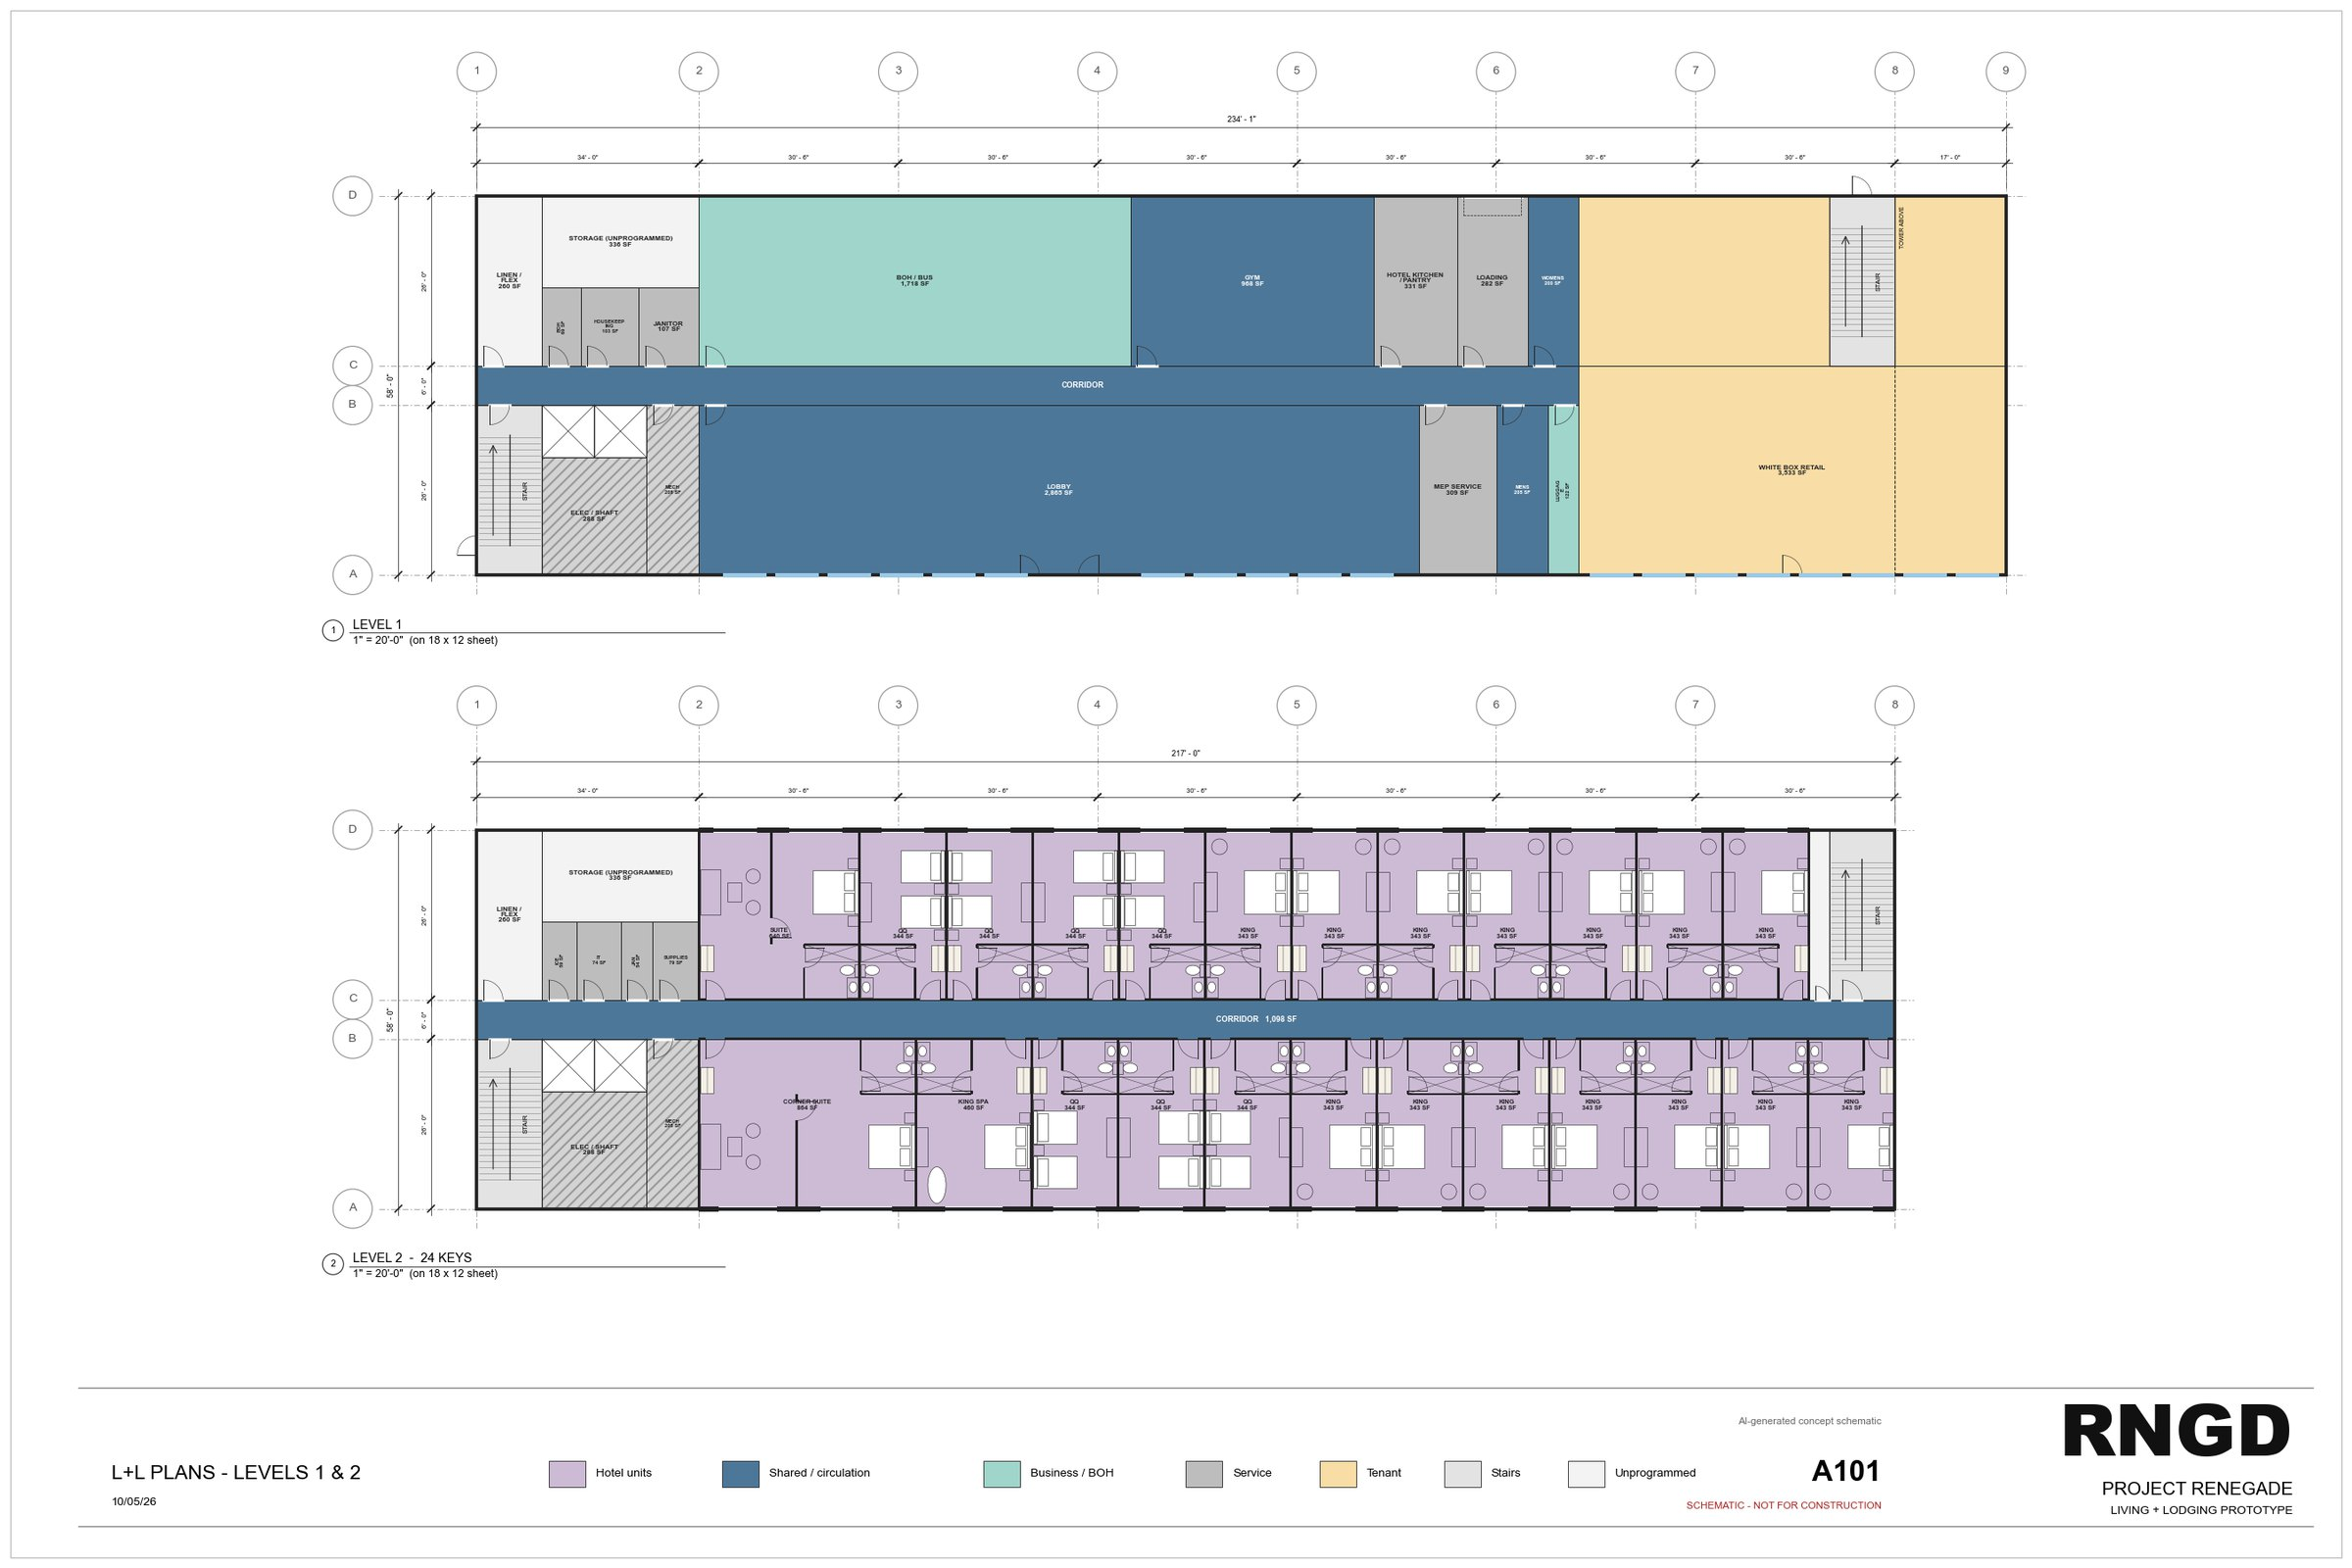
\includegraphics[width=\linewidth]{figures/sheet_A101.jpg}
\caption{Sheet A101: Level 1 and Level 2 plans with column grid (bays of at most 32\,ft), dimension strings, door swings and
fixtures.}
\end{figure}
\begin{figure}[H]
\centering
\begin{subfigure}{0.49\linewidth}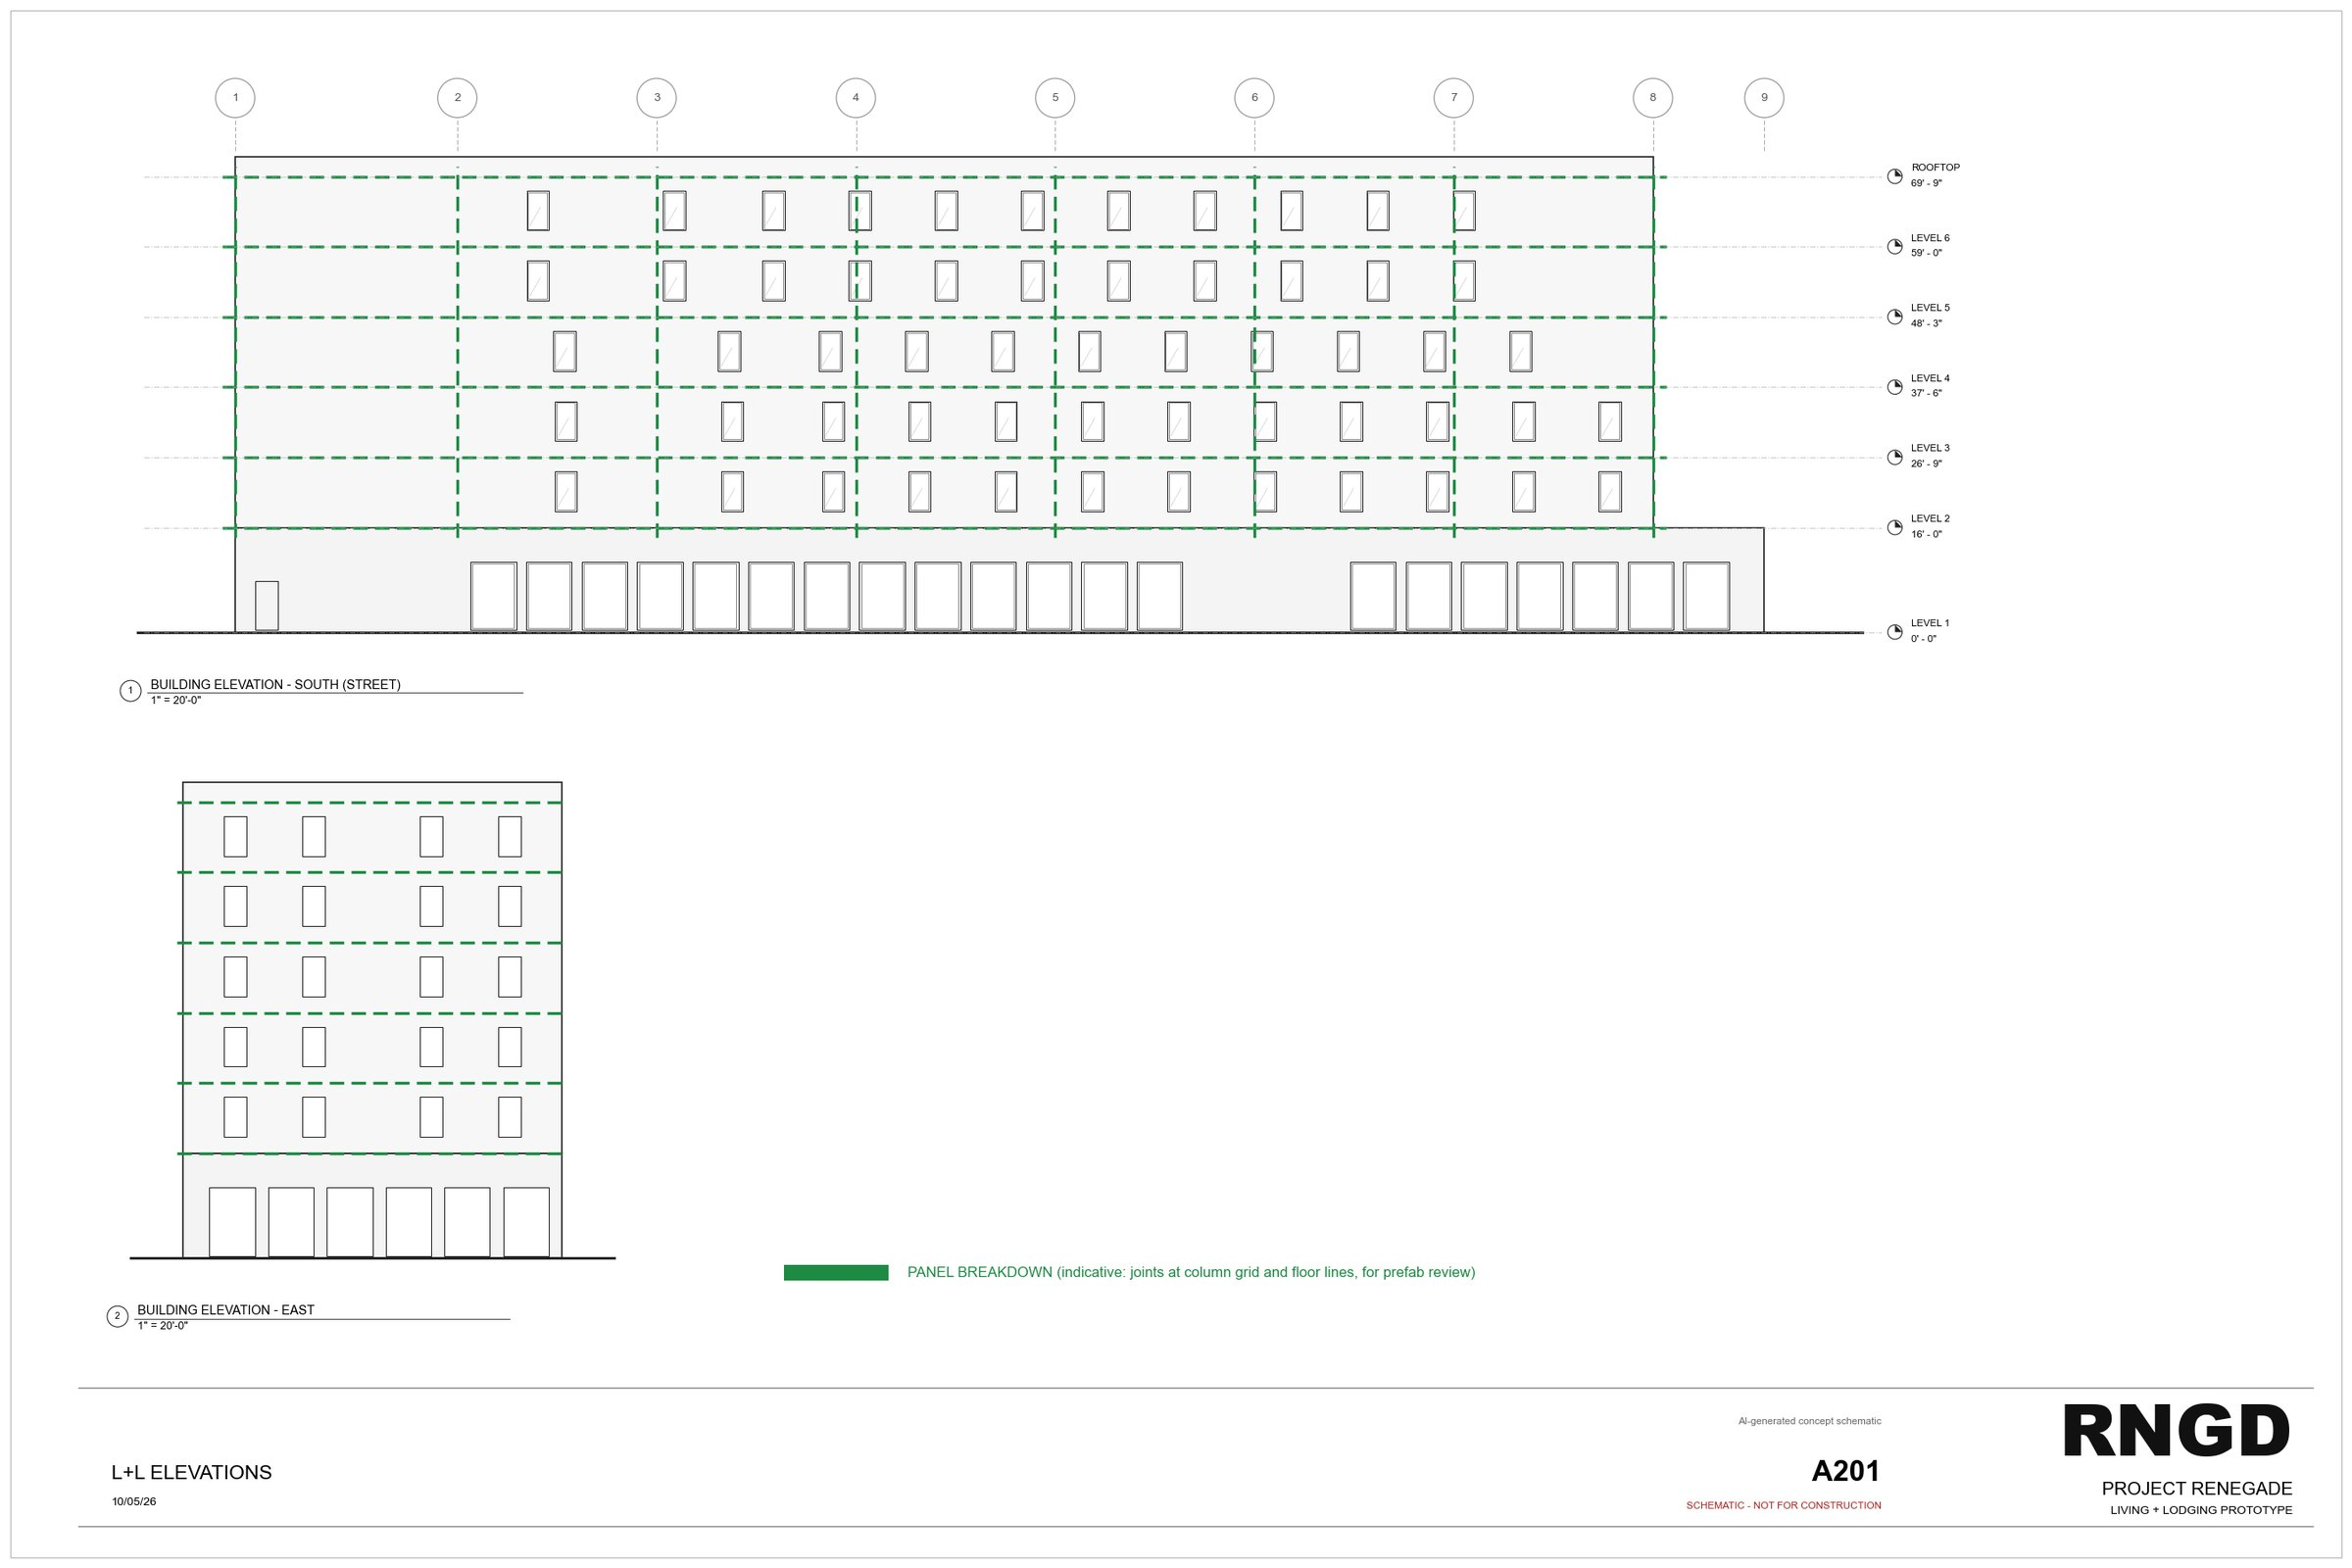
\includegraphics[width=\linewidth]{figures/sheet_A201.jpg}\caption{A201 elevations with panel breakdown.}\end{subfigure}\hfill
\begin{subfigure}{0.49\linewidth}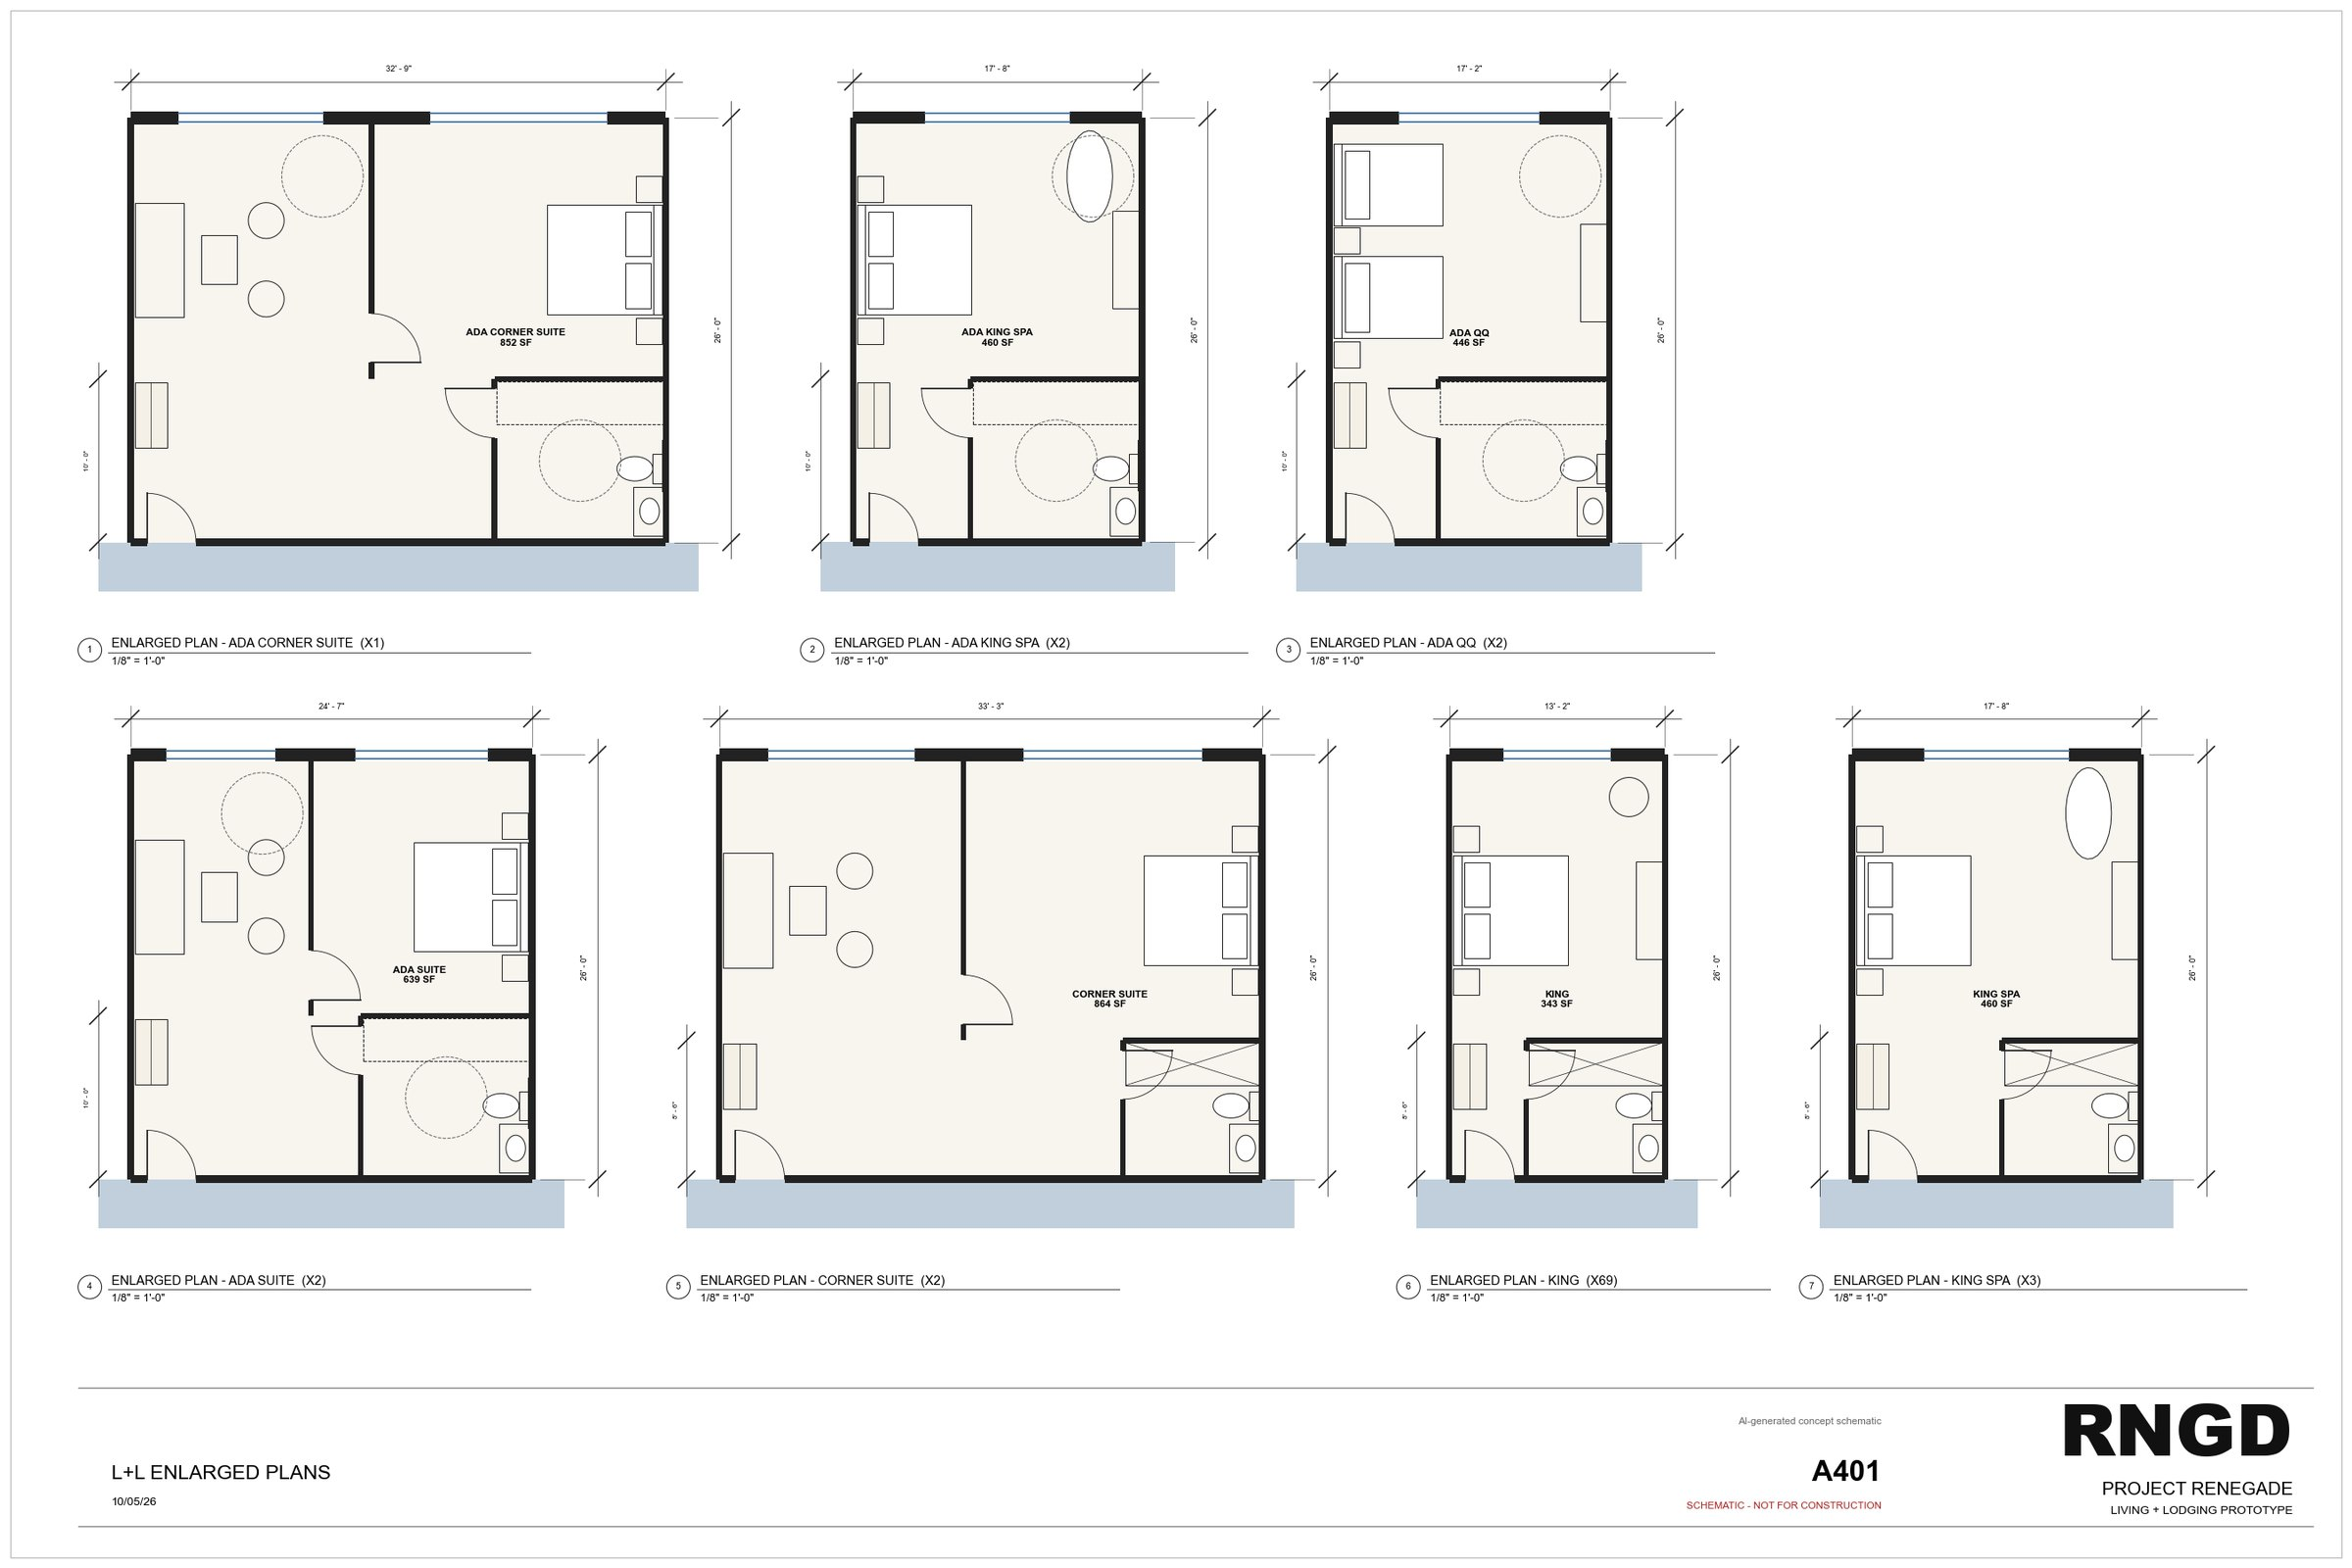
\includegraphics[width=\linewidth]{figures/sheet_A401.jpg}\caption{A401 enlarged unit plans.}\end{subfigure}
\caption{Elevations and enlarged plans.}
\end{figure}

% =====================================================================
% Generated by src/build_paper.py from the optimizer study (reports/walkthrough/optimizer/study.json).
\clearpage
\begingroup\setlength{\tabcolsep}{3.5pt}
% generated by src/build_paper.py from reports/walkthrough/optimizer/study.json

\section{Layout optimization: from the reference GA to the updated optimizer}\label{sec:opt}
\subsection{Summary}
RNGD's design-optimization prototype (B\"u\c{s}ra's genetic algorithm, files in \texttt{QA/}) takes a multi-level 1 ft
site grid and a room program and evolves a corridor and a room placement for 500 generations. This project rebuilt
that optimizer in four steps and measured every step on the same three sites with the same program and the same evaluator
(Table~\ref{tab:optcompare}):
\begin{itemize}
\item \textbf{A, the reference GA} as delivered: 171 rooms placed over the three sites, 24 of the guest rooms without a window.
\item \textbf{C, the updated GA}: a memetic GA on a new architectural decoder, no LLM in the fitness: 197 rooms, 0 without a window, mean fitness 0.928 against 0.863.
\item \textbf{D, systematic search} (the default now): the same decoder, driven by enumeration and pattern search instead of crossover: 192 rooms, 0 without a window, mean fitness 0.922, in 59 s for all three sites and with the same answer on every run.
\end{itemize}
Per site (A $\to$ D): fp1: 61 $\to$ 72 rooms, 7 $\to$ 0 windowless, fitness 0.880 $\to$ 0.950; fp2: 53 $\to$ 60 rooms, 8 $\to$ 0 windowless, fitness 0.860 $\to$ 0.904; fp3: 57 $\to$ 60 rooms, 9 $\to$ 0 windowless, fitness 0.851 $\to$ 0.911. Variant B, the first attempt, kept the reference idea (a GA that moves free corridor segments and packs rooms) and placed 174 rooms in total with 14 windowless guest rooms in 336 s: better scoring alone did not fix the plans, which is why the representation was changed.

The same engine now also runs inside \textbf{Hotel Schematic}, where the shape of the building, the position of the
core and stairs and the number of floors are generated instead of given (Section~\ref{sec:opthotel}).

\subsection{Architecture}
\begin{figure}[H]\centering
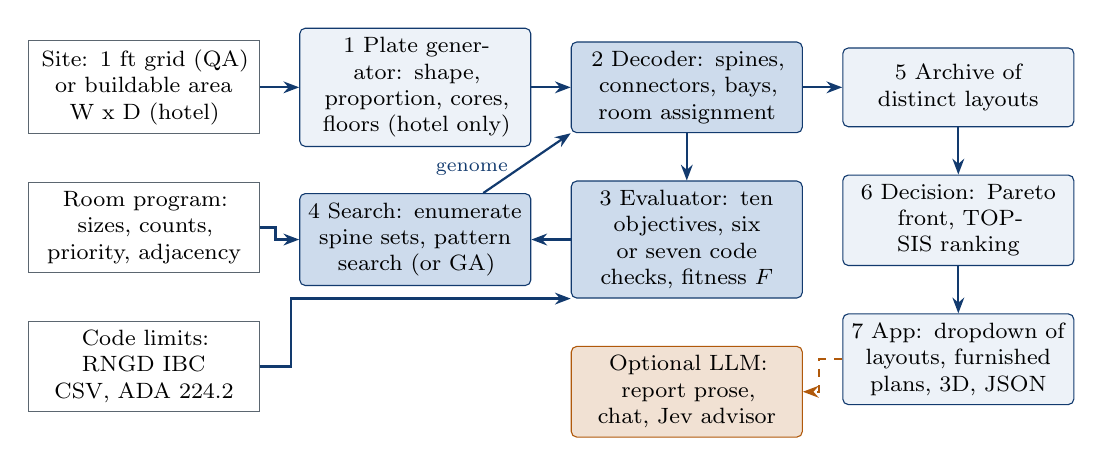
\begin{tikzpicture}[node distance=6mm and 5mm, every node/.style={font=\footnotesize},
 box/.style={draw=bpdeep, fill=bp!8, rounded corners=2pt, align=center, minimum height=10mm, text width=27mm},
 data/.style={draw=muted, fill=white, align=center, minimum height=9mm, text width=27mm},
 ai/.style={box, fill=warn!18, draw=warn}, loop/.style={box, fill=bp!22},
 arr/.style={-{Stealth[length=2mm]}, thick, bpdeep}]
\node[data] (site) {Site: 1 ft grid (QA) or buildable area W x D (hotel)};
\node[data, below=of site] (prog) {Room program: sizes, counts, priority, adjacency};
\node[data, below=of prog] (code) {Code limits: RNGD IBC CSV, ADA 224.2};
\node[box, right=of site] (plate) {1 Plate generator: shape, proportion, cores, floors (hotel only)};
\node[loop, right=of plate] (dec) {2 Decoder: spines, connectors, bays, room assignment};
\node[loop, below=of dec] (eval) {3 Evaluator: ten objectives, six or seven code checks, fitness $F$};
\node[loop, left=of eval] (search) {4 Search: enumerate spine sets, pattern search (or GA)};
\node[box, right=of dec] (arch) {5 Archive of distinct layouts};
\node[box, below=of arch] (dm) {6 Decision: Pareto front, TOPSIS ranking};
\node[box, below=of dm] (ui) {7 App: dropdown of layouts, furnished plans, 3D, JSON};
\node[ai, below=of eval] (llm) {Optional LLM: report prose, chat, Jev advisor};
\draw[arr] (site) -- (plate); \draw[arr] (plate) -- (dec); \draw[arr] (dec) -- (eval);
\draw[arr] (eval) -- (search); \draw[arr] (search) -- node[left, pos=0.4]{\scriptsize genome} (dec.south west);
\draw[arr] (prog.east) -- ++(2mm,0) |- (search.west); \draw[arr] (code.east) -- ++(4mm,0) |- (eval.south west);
\draw[arr] (dec) -- (arch); \draw[arr] (arch) -- (dm); \draw[arr] (dm) -- (ui);
\draw[arr, dashed, warn] (ui.west) -- ++(-3mm,0) |- (llm.east);
\end{tikzpicture}
\caption{Architecture of the layout optimizer. The darker boxes form the optimization loop and are deterministic.
The language model (orange) sits outside the loop: it only writes report prose, answers chat questions, or, if a
TypeSafe key is configured, advises on the final shortlist.}
\end{figure}
{\footnotesize\begin{longtable}{p{0.47cm}p{3.42cm}p{3.61cm}p{7.22cm}}\toprule
\textbf{\#} & \textbf{Component} & \textbf{File} & \textbf{What it does} \\ \midrule \endhead
1 & Plate generator & \texttt{optimize/typology.py} & Turns the hotel program into rooms with BaaP sizes; generates Bar, L, U, T, H and Courtyard plates inside the buildable area, with the elevator core and stairs placed by scheme (ends, centre, knuckle); one site grid per plate. \\
2 & Decoder & \texttt{optimize/planner.py} & Genome $\to$ corridor spines $\to$ orthogonal connectors $\to$ modular bays $\to$ rooms assigned to bays. Every output is a valid plan. \\
3 & Evaluator & \texttt{optimize/metrics.py} & Ten objectives in $[0,1]$, the code checks (exits, exit separation, travel, corridor width, dead end, ADA; stories for the hotel) and the fitness $F$. Limits come from RNGD's IBC CSV. \\
4 & Search & \texttt{optimize/search.py}, \texttt{explore.py} & Systematic enumeration of spine sets plus pattern search (default) or the memetic GA; for the hotel, all plates are screened in parallel processes and the best of each shape refined. \\
5 & Archive & \texttt{optimize/explore.py} & Keeps every distinct layout with its objectives and criteria. \\
6 & Decision & \texttt{optimize/decide.py} & Pareto front and TOPSIS ranking over twelve criteria; optional Jev advisor (TypeSafe) on the shortlist only. \\
7 & Views & \texttt{optimize/plan\_view.py}, \texttt{hotel\_opt\_ui.py}, \texttt{optimizer\_ui.py} & Dropdown of the top or all layouts, furnished interactive plans, 3D massing, comparison charts, JSON export. \\
-- & Reference loader & \texttt{optimize/baseline.py} & Rebuilds the reference designs from \texttt{QA/floorplan*.json} so they are scored by the same evaluator (their shared-wall lengths reproduce the values stored in the files). \\
-- & Report writer & \texttt{optimize/report.py} & One LLM call (\texttt{anthropic/claude-sonnet-5.5} through OpenRouter) writes the prose of the per-run PDF from the computed data and retrieved code passages; every number in its text is traced back to the data. \\
\bottomrule\end{longtable}}\addtocounter{table}{-1}
Only the last row uses a language model. Steps 1 to 6 are plain Python on NumPy, SciPy and scikit-image arrays, so the
same inputs always give the same layouts and the same ranking.

\subsection{What was wrong, and how it was solved}
The problems below were seen in the reference results, in the first version of this app's optimizer (which followed the
same idea and added an LLM reviewer to the fitness) and in the team review of 10/08/2026.
{\footnotesize\begin{longtable}{p{3.13cm}p{3.52cm}p{4.66cm}p{3.42cm}}
\toprule
\textbf{Observed problem} & \textbf{Cause} & \textbf{What was changed} & \textbf{Evidence in this run} \\ \midrule \endhead
Guest rooms with no window; corridors loaded on one side only (review in the 10/08 meeting). & The corridor genome places segments anywhere; rooms are packed wherever they touch a corridor, so the distance to the facade is left to chance. & Decoder: corridor spines are chosen from lines scored for double-loaded window rooms (score $s(k)$); guest rooms may only take bays with a window (hard rule). & Windowless guest rooms over the three sites: 24 (A) $\to$ 0 (D). \\
Floor area left unused; rooms rotated or isolated. & Rooms are placed one by one as free rectangles, so leftovers between rooms cannot be used. & Modular bays of one room frontage $M$ along the whole corridor; rooms take whole bays, the last bay absorbs the remainder; unused bays are reported as flex space. & Unused share and corridor share per variant in Table~\ref{tab:optcompare}. \\
Not clear whether the requested keys can fit at all. & No bound was computed; the GA simply reports what it placed. & Area and window upper bounds, shown next to every result. & Table~\ref{tab:bounds}. \\
Crossover produces plans that do not make sense; slow convergence. & Half of one plan spliced onto half of another: the value of a corridor depends on the other corridors. & Search over a small structured space: enumerate spine sets, then first-improvement pattern search. The GA is kept as an option and now runs on the same decoder. & At the same budget D is within 0.010 fitness of the GA (C) with no crossover and no population: 192 against 197 rooms. Most of the gain over A comes from the decoder, not from the search. \\
With crossing corridors, facade strips stayed empty (seen on the square site fp2 in the first version of the new decoder: 39 rooms). & Bays were built corridor by corridor, so the windowless interior side of the first corridor took the strip that the next corridor's window rooms needed. & Two passes over all corridors: window bays first, windowless bays in what is left. & fp2: 60 rooms (D) and 62 (C), all guest rooms with a window. \\
Corridor stubs beyond the last room; dead ends over the 50 ft limit. & Spines were cut to the bays they could serve, not to the rooms actually placed. & After the assignment each spine is cut back to the doors and junctions it serves; the dead end is measured to the nearest exit door or through-route. & Longest dead end, D: 46 ft; A: 41 ft (same measure). \\
Runs take minutes; results change between runs. & 500 generations in the reference; an LLM reviewer inside the fitness in the earlier version of this app (about 10 minutes, cloud calls). & No LLM in the fitness; deterministic seeds; cached static scores in the assignment; plates evaluated in parallel processes. & Variant D: 59 s for the three sites; identical result on a repeat run: yes. \\
Egress and accessibility not part of the score. & The reference score rewards placed rooms and contiguity. & Ten objectives including exit travel, dead ends, ADA Table 224.2 count and dispersion, core access; limits read from RNGD's IBC CSV. & All variants pass the checks on these sites; the checks are now reported for every layout. \\
The shape, the core and the floor count are inputs. & The grid fixes the L-shaped plate and both cores. & Hotel Schematic: plates (six shapes), core schemes (three) and the floor count are generated and searched; a dropdown lists the top or all layouts. & 740 distinct layouts in 36 s (Section~\ref{sec:opthotel}). \\
\bottomrule
\end{longtable}}\addtocounter{table}{-1}


\subsection{The mathematics}
\label{sec:optmath}
\paragraph{Problem.} A site is a stack of $L$ levels of 1 ft cells. On each level a set $\Omega$ of cells is
\emph{placeable}; cores (stairs, elevators) and structure are fixed in the QA sites and generated for the hotel. The program
is a list of room instances $i = 1..N$, each with a type $t(i)$, nominal frontage $f_i$ and depth $d_i$ (area
$\bar a_i = f_i d_i$), a priority $p_i$, a set of allowed levels and flags (needs a window, wants a corner, wants to be near a
core). A layout chooses a corridor $C \subset \Omega$ (the same on every level, so floors stack) and an axis-aligned rectangle
for some of the rooms, such that rectangles do not overlap each other or $C$, lie inside $\Omega$, and each room has a door on
$C$. The goal is to maximise the fitness $F$ below.

\paragraph{Decoder: from a short genome to a full layout.} The search never moves rooms directly. It works on a genome
$g \in [0,1]^{44+N}$ (ten candidate spines with four genes each: two trims, a shift, an on/off gene; four connector genes;
one order key per room) and the decoder builds the layout:
\begin{enumerate}
\item \textbf{Module.} The bay width is the weighted median guest-room frontage,
$M = \operatorname{median}_w\{f_t\}$ with weights equal to the room counts; $D$ is the median guest-room depth and $w$ the
corridor width.
\item \textbf{Candidate spines.} Every row and column $k$ that can hold a straight corridor band gets the score
\[ s(k) = \sum_{x \in \text{band}(k)} \big[\, g_a(x) + g_b(x) + 1.5\,n_a(x) + 1.5\,n_b(x) + 0.5\,r_a(x) + 0.5\,r_b(x) \,\big], \]
where, for the two sides $a$ and $b$ of the band at position $x$, $g=1$ if a room at least $0.92\,d_{\min}$ deep fits,
$n=1$ if in addition the facade is about one room depth away (a window room), and $r=1$ if it is within the deepest room's
depth. So a line that is double-loaded with window rooms on both sides scores $2 \times (1 + 1.5 + 0.5) = 6$ per foot, a
single-loaded line 3, and a line through deep space with no facade 2. The best non-overlapping lines (at least $d_{\min}+w$
apart) become the ten candidates.
\item \textbf{Connectors.} Active spines are trimmed to their last room and joined to each other and to every core with
orthogonal L-shaped paths (never diagonal); pieces that stay unconnected are dropped.
\item \textbf{Bays.} Each side of each straight corridor run of length $\ell$ is cut into
$n = \lfloor \ell / M \rfloor$ bays. The remainder $\rho = \ell - nM$ is absorbed by the last bay if $\rho < 0.4M$ and becomes
a narrow bay otherwise. A bay has a window if its back wall is on the facade. Bays are built in two passes over all
corridors, window bays first and windowless bays in what is left, so the interior side of one corridor never takes
the facade strip that another corridor's window rooms need.
\item \textbf{Assignment.} Rooms are taken in the order of $0.06\,p_i + g_i$ (priority, then the order key) and each takes
\[ k_i = \max\!\Big(\operatorname{round}\frac{\bar a_i}{M D},\ \Big\lceil \frac{0.85 f_i}{M} \Big\rceil\Big) \]
consecutive free bays on one allowed level, the run with the highest score
\begin{align*} \sigma ={}& W_{\text{ext}}\,[\text{window}] - W_{\text{nw}}\,[\text{no window}] + W_{\text{corner}}\,[\text{corner}]
+ W_{\text{core}}\Big(1 - \tfrac{\min(\delta,150)}{150}\Big) + W_{\text{adj}}\,A \\
&+ W_{\text{stack}}\,\tfrac{\min(S,2)}{2} + W_{\text{grp}}\,[\text{same type next door}] - 1.2\max(0, o - 1.2),
\end{align*}
with $\delta$ the corridor distance from the door to the nearest core, $A$ the adjacency credit, $S$ the number of floors
with the same room type in the same bay, and $o$ the ratio of the bay area to the room's nominal area. Two hard rules apply:
a guest room is only placed where every bay has a window, and only if the run gives at least 85\% of its nominal frontage
and depth.
\end{enumerate}
After the assignment, each spine is cut back to what it serves (the doors of placed rooms and its junctions with
other corridors and cores), which removes corridor stubs and shortens dead ends. The dead end $E$ is the longest
corridor distance from any corridor cell to the nearest exit door or through-route between two exits.

Every decoded layout is therefore valid by construction (straight corridors, rooms perpendicular to them, no overlaps, all
rooms on the corridor), and the search only has to decide \emph{which} corridors exist and \emph{in what order} rooms claim
bays.

\paragraph{Fitness.} Ten objectives $f_k \in [0,1]$ (1 is best) are combined with weights $w_k$:
\[ F = \frac{\sum_k w_k f_k}{\sum_k w_k} \; - \; \tfrac12 \max\!\big(0,\ \min(n_c, 2) - c\big), \]
where $n_c$ is the number of cores and $c$ the number the corridor reaches (an exit that is not connected costs half the
scale). With $\rho$ the corridor share of the plate, $T$ the longest exit travel and $E$ the longest dead end:
\begingroup\small\begin{align*}
f_{\text{place}} &= \frac{\sum_{i\ \text{placed}} p_i \min(a_i, \bar a_i)}{\sum_{i} p_i \bar a_i}, &
f_{\text{day}} &= \frac{\#\{\text{rooms needing a window that have one}\}}{\#\{\text{rooms needing a window}\}}, \\
f_{\text{eff}} &= \operatorname{clip}\!\Big(1 - \frac{\rho}{0.30}\Big), &
f_{\text{egress}} &= 1 - \tfrac12 \min\!\Big(1, \frac{(T - 250)^+}{250}\Big) - \tfrac12 \min\!\Big(1, \frac{(E - 50)^+}{50}\Big), \\
f_{\text{ada}} &= \min\!\Big(1, \frac{n_{\text{ADA}}}{n_{224.2}}\Big)\cdot\min\!\Big(1, \frac{\text{floors with ADA}}{\text{target}}\Big), &
f_{\text{core}} &= \operatorname{mean}_i \Big(1 - \frac{\min(\delta_i, 120)}{120}\Big), \\
f_{\text{adj}} &= \frac{\sum_j \omega_j \max\big(0,\ 1 - (\Delta_j - m_j)^+/m_j\big)}{\sum_j \omega_j}, &
f_{\text{corner}} &= \frac{\#\{\text{corner rooms on a corner}\}}{\#\{\text{corner rooms}\}}, \\
f_{\text{bal}} &= \operatorname{clip}\!\Big(1 - \frac{\operatorname{sd}(K_\ell)}{\operatorname{mean}(K_\ell)}\Big), &
f_{\text{comp}} &= \operatorname{clip}\!\Big(\frac{2 S_{\text{shared}}}{0.6\, P_{\text{rooms}}}\Big).
\end{align*}\endgroup
Here $a_i$ is the drawn area (credit is capped at the nominal area, so an oversized room is not worth more),
$\Delta_j$ the distance between the two rooms of adjacency $j$ with allowed distance $m_j$, $K_\ell$ the keys on guest floor
$\ell$, $S_{\text{shared}}$ the total length of walls shared by two rooms and $P_{\text{rooms}}$ the total room perimeter.
The limits 250 ft (exit travel) and 50 ft (dead end) are read from RNGD's IBC rule CSV. The weights are
placement 0.3, daylight 0.14, efficiency 0.1, egress 0.12, ada 0.08, core access 0.07, adjacency 0.07, corner 0.03, balance 0.05, compactness 0.04. There is no language model in $F$: it is arithmetic on the geometry.

\paragraph{Upper bounds (can the keys fit at all?).} Two bounds hold for any layout, whatever the algorithm.
A corridor of width $w$ serves at most two room depths, so at least $w/(2D+w)$ of the used floor is corridor:
\[ K \le K_{\text{area}} = \Big\lfloor \frac{L\,|\Omega|\,\big(1 - \tfrac{w}{2D+w}\big)}{\bar a} \Big\rfloor . \]
If every guest room needs a window, the rooms of one floor share the facade length $P_f$:
\[ K \le K_{\text{window}} = L \Big\lfloor \frac{P_f}{\bar f} \Big\rfloor . \]
For a generated hotel plate with corridor length $R$ and cores taking a frontage $c_f$, the bound per floor is
$\lfloor (2R - c_f)/M \rfloor$. The bounds are loose (they ignore corners and the public rooms), but a request above them
is impossible, and a result close to them is close to the best any search can do.

\paragraph{Search.} With $m$ candidate spines the decoder is driven by a subset of them, so the first stage enumerates
\[ 1 + \sum_{k=1}^{4} \binom{\min(m,7)}{k} \le 1 + 7 + 21 + 35 + 35 = 99 \]
spine sets (all spines, and every set of up to four of the seven best), with rooms in priority order. The second stage
starts from the three best distinct layouts and repeats: generate the neighbours (switch one spine on or off: 10 moves; trim
either end or shift an active spine: 4 moves each; new connector elbows; four room-order nudges), evaluate them in a seeded
random order, and accept the first one with $F' > F + 10^{-6}$. When all three starts are local optima, the rest of the budget is spent on iterated local search: the best
layout is ``kicked'' with two moves at once, improved again by the same pattern search, and kept only if it beats
the best so far. The total budget is $PG$ evaluations ($P$ = population, $G$ = generations, kept as the budget
controls), the same as the GA's. The genetic algorithm (variant C)
evaluates $P(G+1)$ layouts plus local-search steps, here about 804. Crossover is not used in the systematic search:
splicing the corridor genes of one plan with the room order of another seldom gives a better plan, because the value of a
corridor depends on which other corridors exist.

\paragraph{Plate generation (hotel).} For $K$ keys on $F$ guest floors the busiest level needs net area $A$; with slack
$\varsigma = 1.04$, core area $A_c$ and packing efficiency $\eta = 0.93$ the corridor length to provide is
\[ R = \frac{\varsigma A + A_c}{2 D \eta}. \]
Each shape with bounding box $a \times b$ and wing depth $W_d = 2D + w$ (58 ft) offers
$R_{\text{Bar}} = a$, $R_{\text{L}} = R_{\text{T}} = a + b - W_d$, $R_{\text{U}} = a + 2b - 2W_d$,
$R_{\text{H}} = a + 2b - 2W_d$ and $R_{\text{Courtyard}} = 2a + 2b - 4W_d$; the generator solves $R_{\text{shape}}(a, \beta a) \ge R$
for the smallest $a$ at aspect ratios $\beta \in \{0.6, 1\}$ and clips the result to the buildable area in both
orientations. The elevator count is $e = \max(2, \lceil K/75 \rceil)$, and the two stairs of the ``centre core'' scheme are
the pair of wing-end positions with the largest distance between them (exit separation, short dead ends).

\paragraph{Decision.} Each layout $j$ has a vector of twelve criteria $x_{j1..12}$ (keys, gross SF per key, facade per key,
height, corridor share, dead end, code checks passed and others). Layout $j$ is \emph{dominated} if another layout is at
least as good on every criterion and strictly better on one; the rest form the Pareto front. TOPSIS then ranks all layouts:
\[ r_{jq} = \frac{x_{jq}}{\sqrt{\sum_j x_{jq}^2}}, \quad v_{jq} = \frac{\lambda_q}{\sum_q \lambda_q}\, r_{jq}, \quad
d_j^{\pm} = \sqrt{\sum_q (v_{jq} - v_q^{\pm})^2}, \quad C_j = \frac{d_j^-}{d_j^+ + d_j^-} \in [0,1], \]
where $v_q^+$ is the best and $v_q^-$ the worst value of criterion $q$ over all layouts and $\lambda_q$ the weight from the
chosen preset (Balanced, Most keys, Lowest cost, Guest experience, Low-rise) or the sliders. The layout with the largest
$C_j$ is ranked first.


\subsection{Results on the three QA sites}\label{sec:optqa}
All variants use \texttt{QA/rooms\_hotel.json} (72 rooms on three levels) and are scored by the same evaluator. Variants
B, C and D were run with population 24 and 30 generations as the budget, seed 7, no LLM.
For A the search time is not stored in the files; its history holds 500 generations.
\begingroup\captionof{table}{Reference GA and the three later variants. ``No window'' counts guest rooms without a facade wall; ``Unused'' is the share of placeable area that is neither room nor corridor; ``Checks'' are the code checks passed.}\label{tab:optcompare}\endgroup
{\footnotesize\begin{longtable}{p{0.76cm}p{2.75cm}p{1.04cm}p{1.14cm}p{1.04cm}p{1.14cm}p{1.04cm}p{1.23cm}p{0.95cm}p{1.42cm}p{0.95cm}}
\toprule
\textbf{Site} & \textbf{Variant} & \textbf{Rooms} & \textbf{No window} & \textbf{Fitness} & \textbf{Corridor} & \textbf{Unused} & \textbf{Dead end ft} & \textbf{Checks} & \textbf{Evaluated} & \textbf{Time} \\ \midrule \endhead
fp1 & A Reference GA & 61/72 & 7 & 0.880 & 0.151 & 0.16 & 33 & 6/6 & 500 gen. & n/a \\
 & B GA, free-form & 53/72 & 3 & 0.880 & 0.100 & 0.29 & 55 & 5/6 & 804 & 119 s \\
 & C Updated GA & 72/72 & 0 & 0.954 & 0.101 & 0.09 & 27 & 6/6 & 804 & 24 s \\
 & D Systematic & 72/72 & 0 & 0.950 & 0.101 & 0.09 & 25 & 6/6 & 695 & 20 s \\ \midrule
fp2 & A Reference GA & 53/72 & 8 & 0.860 & 0.117 & 0.26 & 31 & 6/6 & 500 gen. & n/a \\
 & B GA, free-form & 60/72 & 8 & 0.893 & 0.111 & 0.19 & 36 & 6/6 & 804 & 102 s \\
 & C Updated GA & 62/72 & 0 & 0.908 & 0.146 & 0.06 & 43 & 6/6 & 804 & 22 s \\
 & D Systematic & 60/72 & 0 & 0.904 & 0.145 & 0.09 & 46 & 6/6 & 637 & 17 s \\ \midrule
fp3 & A Reference GA & 57/72 & 9 & 0.851 & 0.157 & 0.18 & 41 & 6/6 & 500 gen. & n/a \\
 & B GA, free-form & 61/72 & 3 & 0.894 & 0.120 & 0.18 & 33 & 6/6 & 804 & 115 s \\
 & C Updated GA & 63/72 & 0 & 0.921 & 0.122 & 0.11 & 35 & 6/6 & 804 & 26 s \\
 & D Systematic & 60/72 & 0 & 0.911 & 0.119 & 0.09 & 29 & 6/6 & 683 & 21 s \\
\bottomrule
\end{longtable}}\addtocounter{table}{-1}
\begingroup\captionof{table}{Upper bounds on the number of keys (Section~\ref{sec:optmath}) against what was asked and placed.}\label{tab:bounds}\endgroup
{\footnotesize\begin{longtable}{p{0.76cm}p{1.52cm}p{1.23cm}p{1.42cm}p{1.33cm}p{1.52cm}p{0.95cm}p{1.14cm}p{0.95cm}p{0.85cm}p{0.85cm}}
\toprule
\textbf{Site} & \textbf{Placeable SF / level} & \textbf{Program SF} & \textbf{Program / placeable} & \textbf{Facade ft / level} & \textbf{Mean key frontage ft} & \textbf{$K_{\text{area}}$} & \textbf{$K_{\text{window}}$} & \textbf{Keys asked} & \textbf{Keys A} & \textbf{Keys D} \\ \midrule \endhead
fp1 & 9,640 & 23,310 & 0.81 & 489 & 12.9 & 80 & 111 & 69 & 58 & 69 \\
fp2 & 9,446 & 23,310 & 0.82 & 410 & 12.9 & 78 & 93 & 69 & 50 & 57 \\
fp3 & 9,412 & 23,310 & 0.83 & 519 & 12.9 & 78 & 120 & 69 & 54 & 57 \\
\bottomrule
\end{longtable}}\addtocounter{table}{-1}
\begin{figure}[H]\centering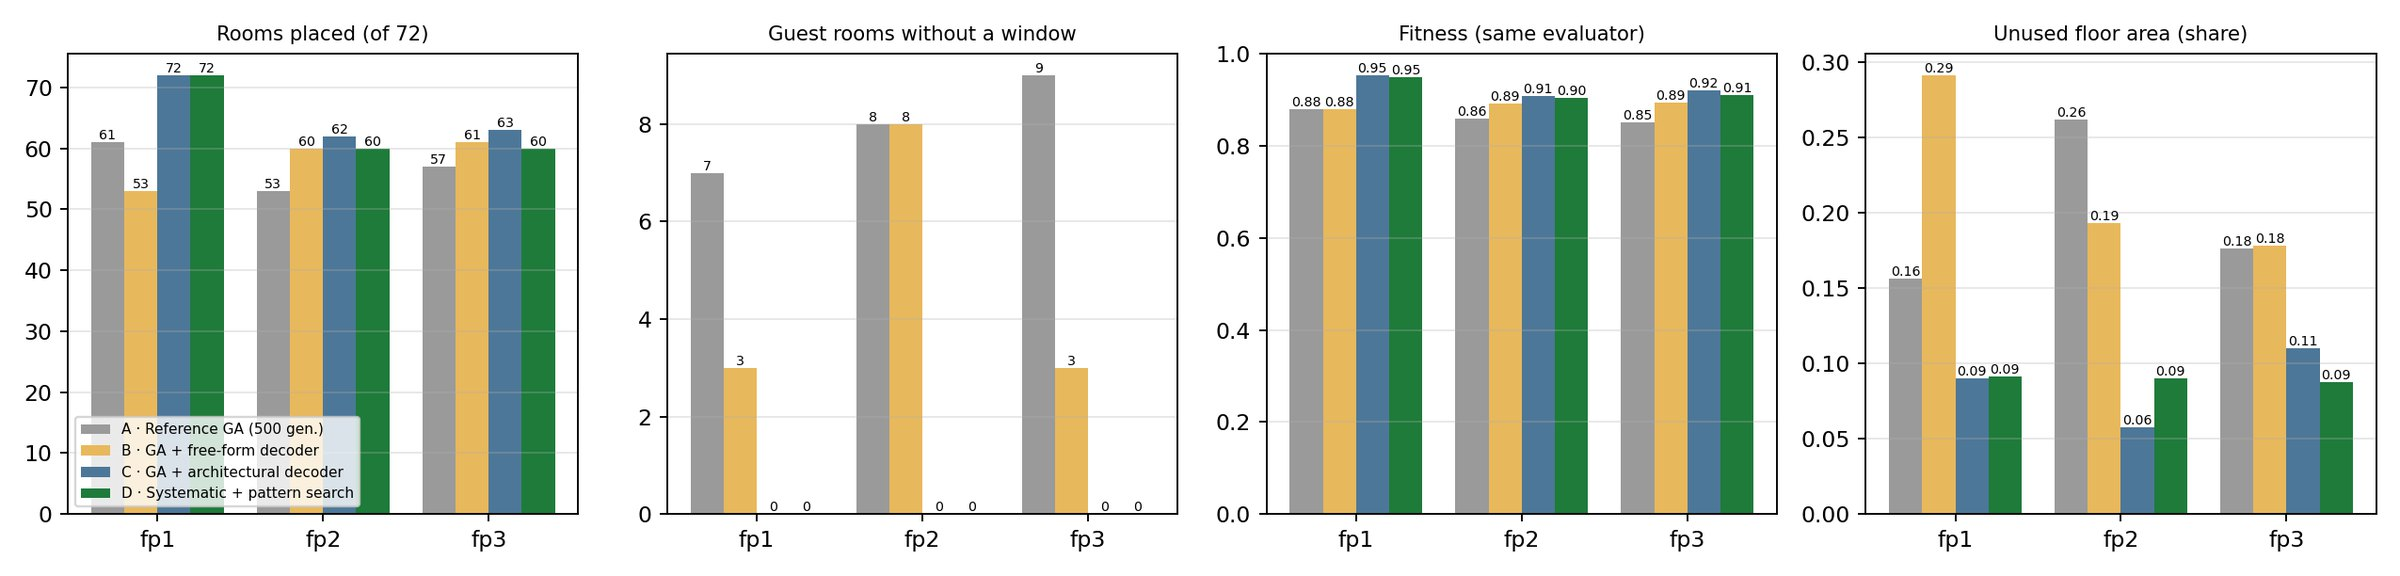
\includegraphics[width=\linewidth,keepaspectratio,height=0.30\textheight]{figures/opt_compare_bars.jpg}\caption{The four variants on the three sites (same program, same evaluator).}\end{figure}
\begin{figure}[H]\centering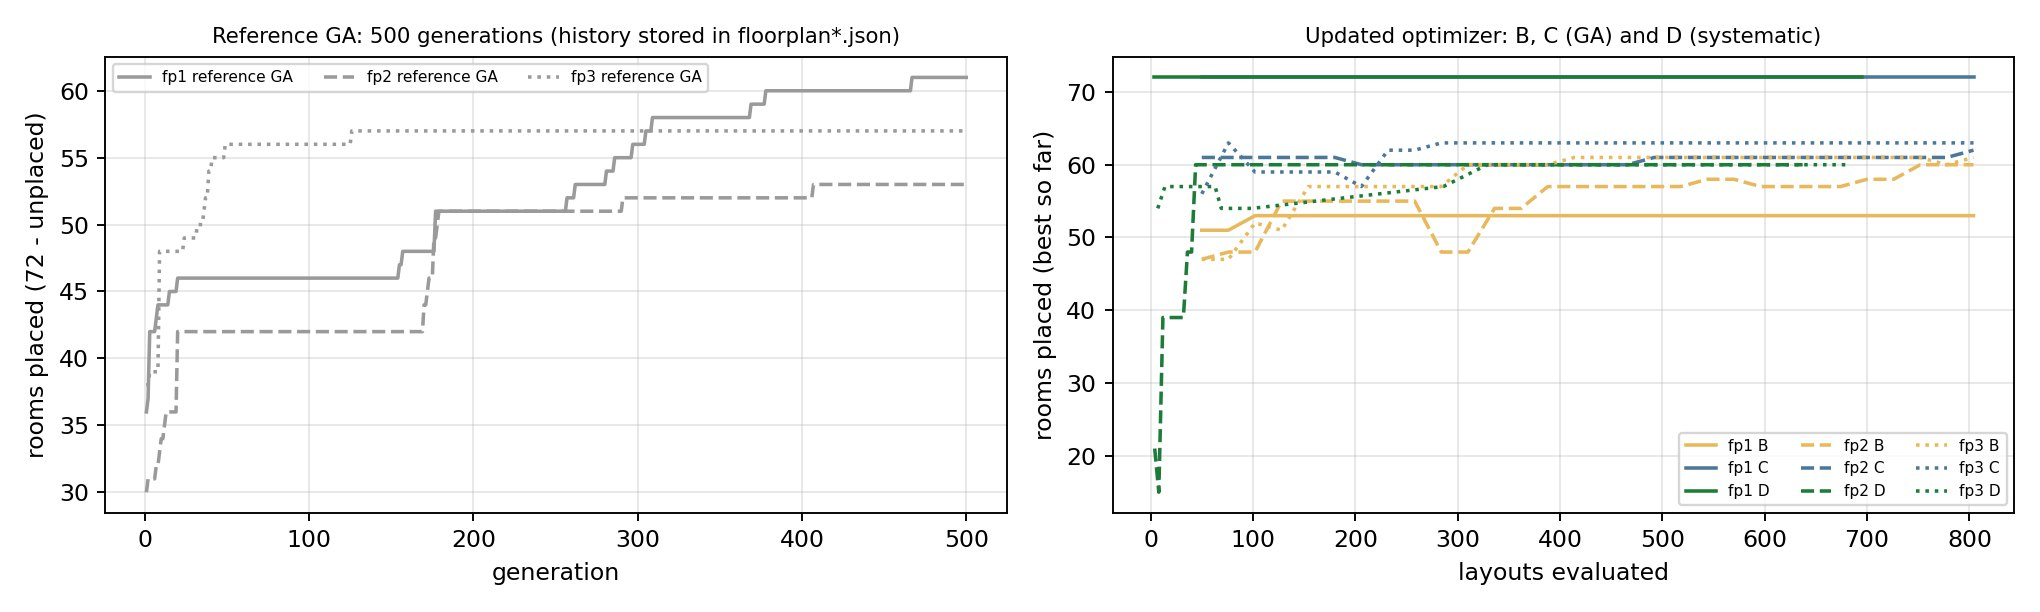
\includegraphics[width=\linewidth,keepaspectratio,height=0.30\textheight]{figures/opt_convergence.jpg}\caption{Left: rooms placed by the reference GA over its generations (from the history in the delivered files). Right: best rooms placed against layouts evaluated for the later variants.}\end{figure}
\begin{figure}[H]\centering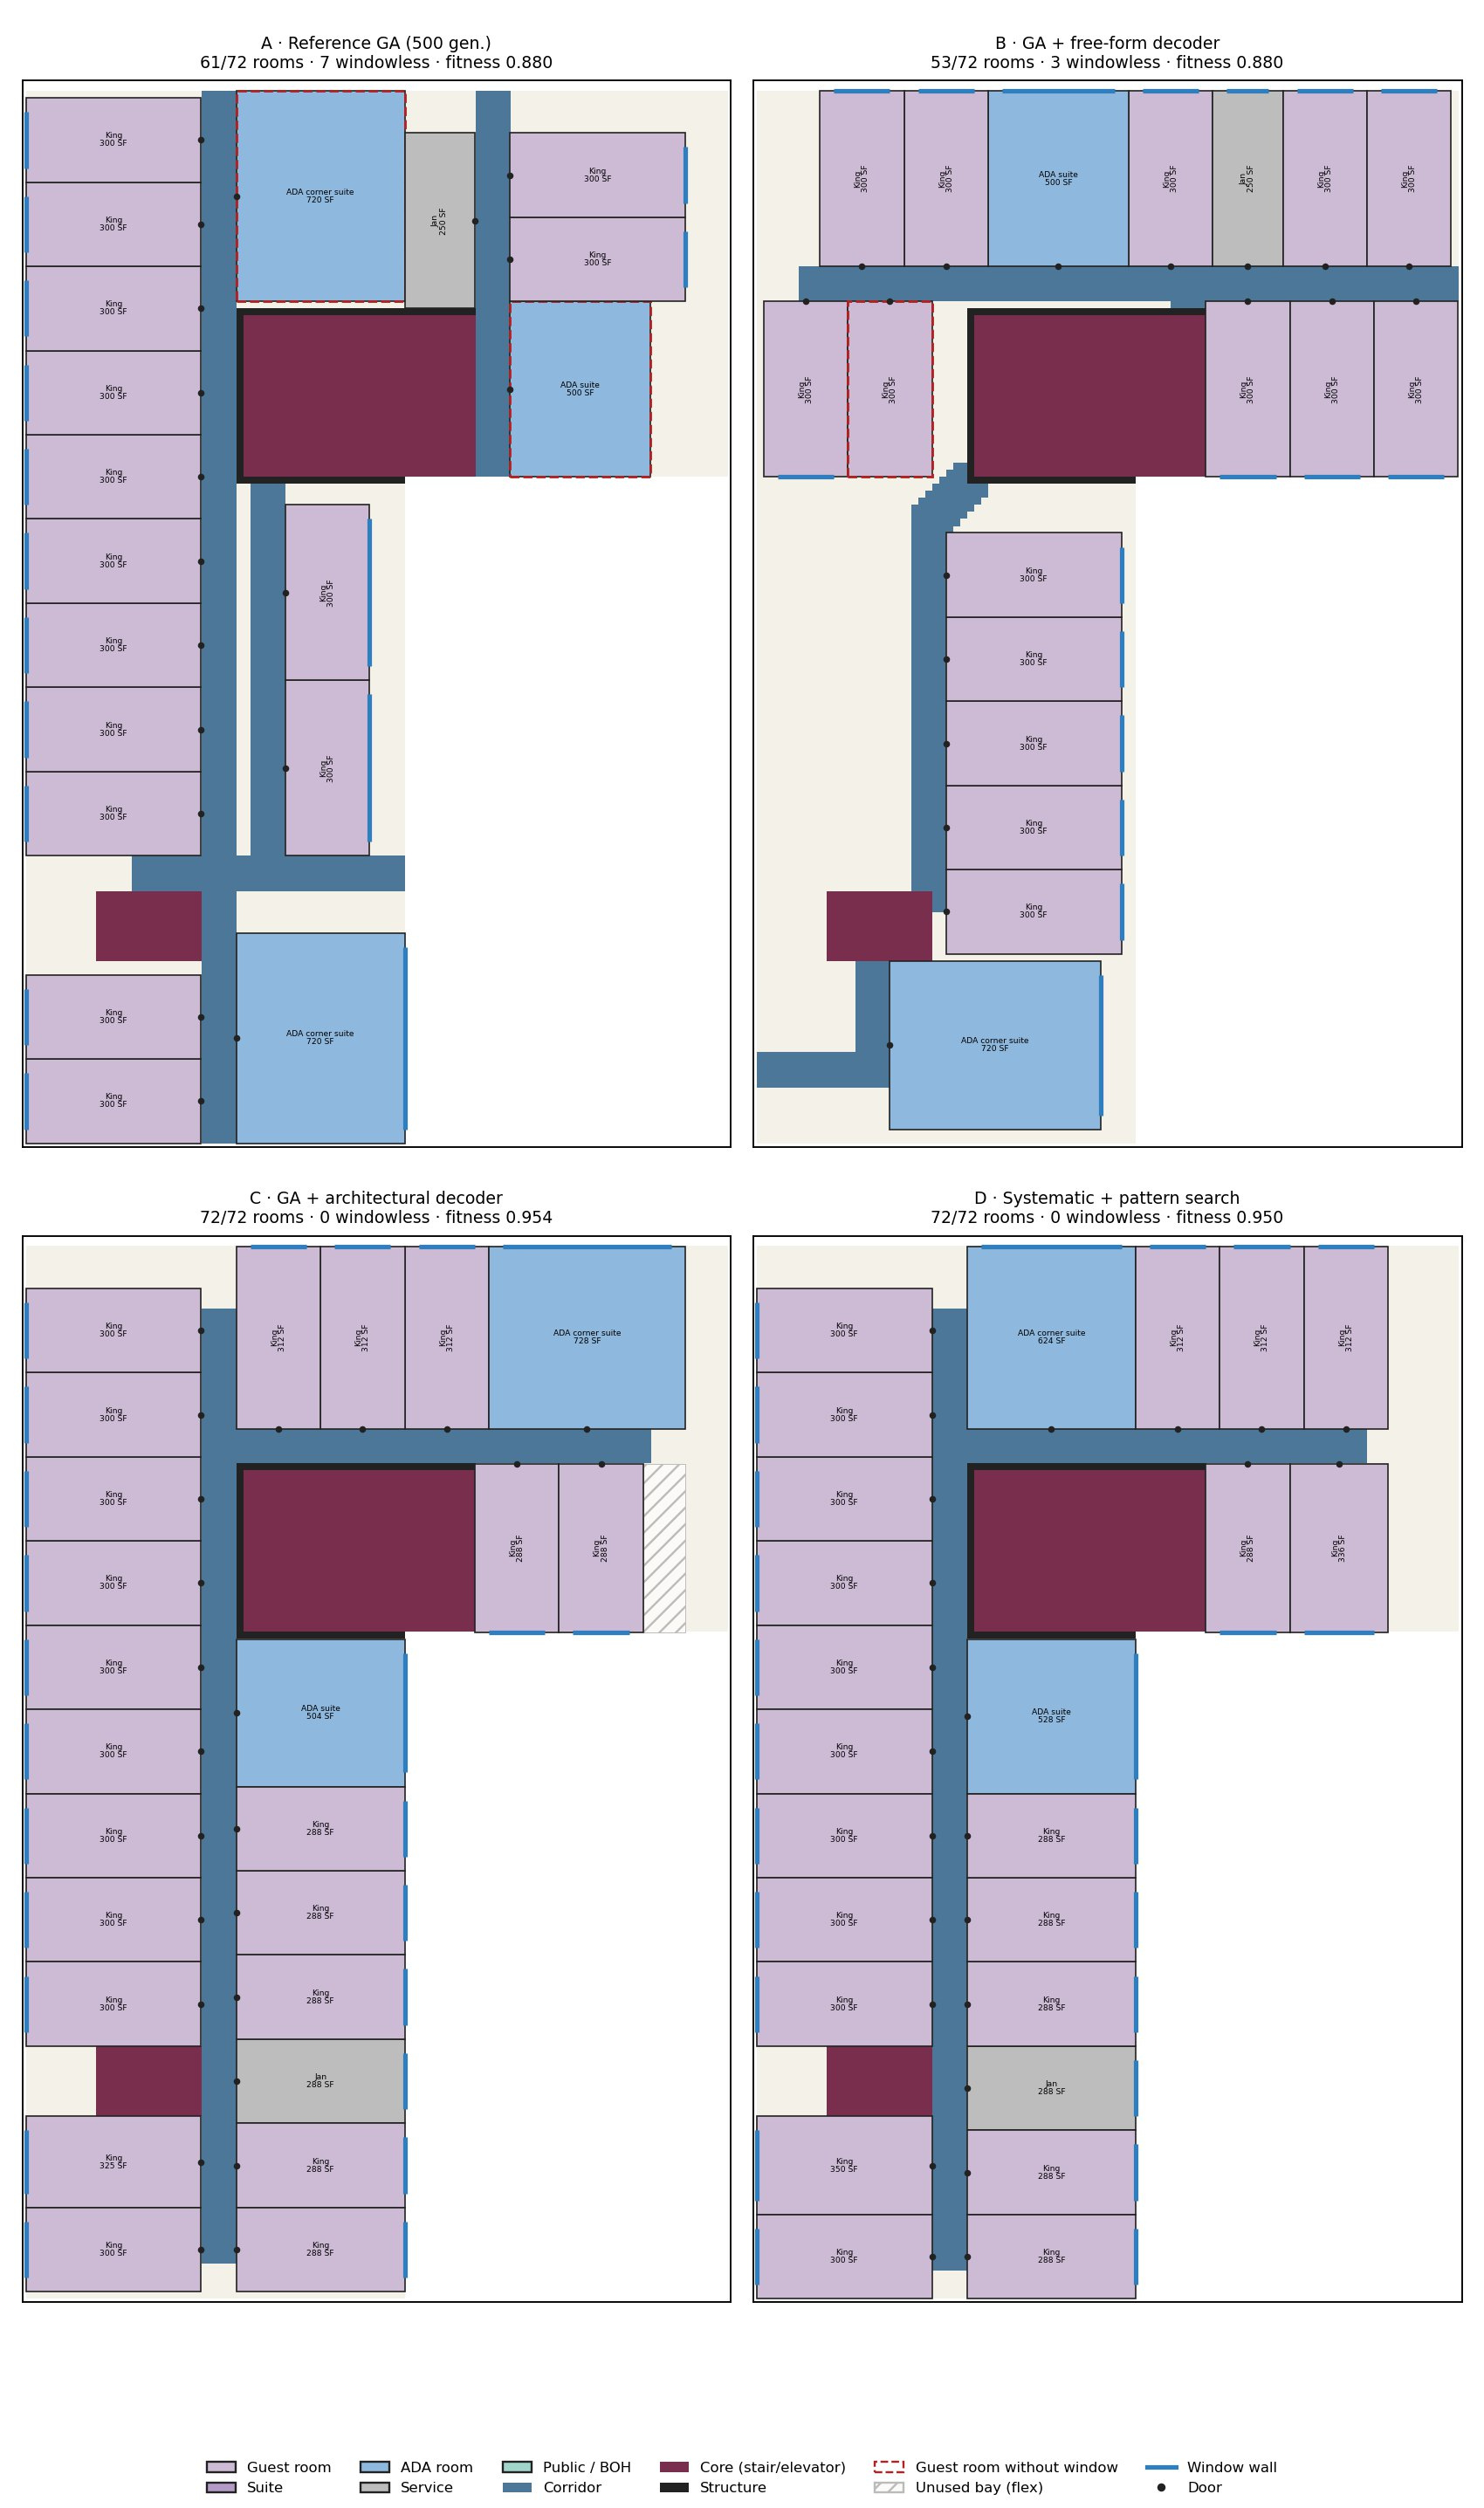
\includegraphics[width=\linewidth,keepaspectratio,height=0.80\textheight]{figures/opt_compare_fp1.jpg}\caption{Site fp1, Level 2, same program and same evaluator. Blue lines are window walls; a red dashed outline marks a guest room with no window; hatched bays are unused.}\end{figure}
\begin{figure}[H]\centering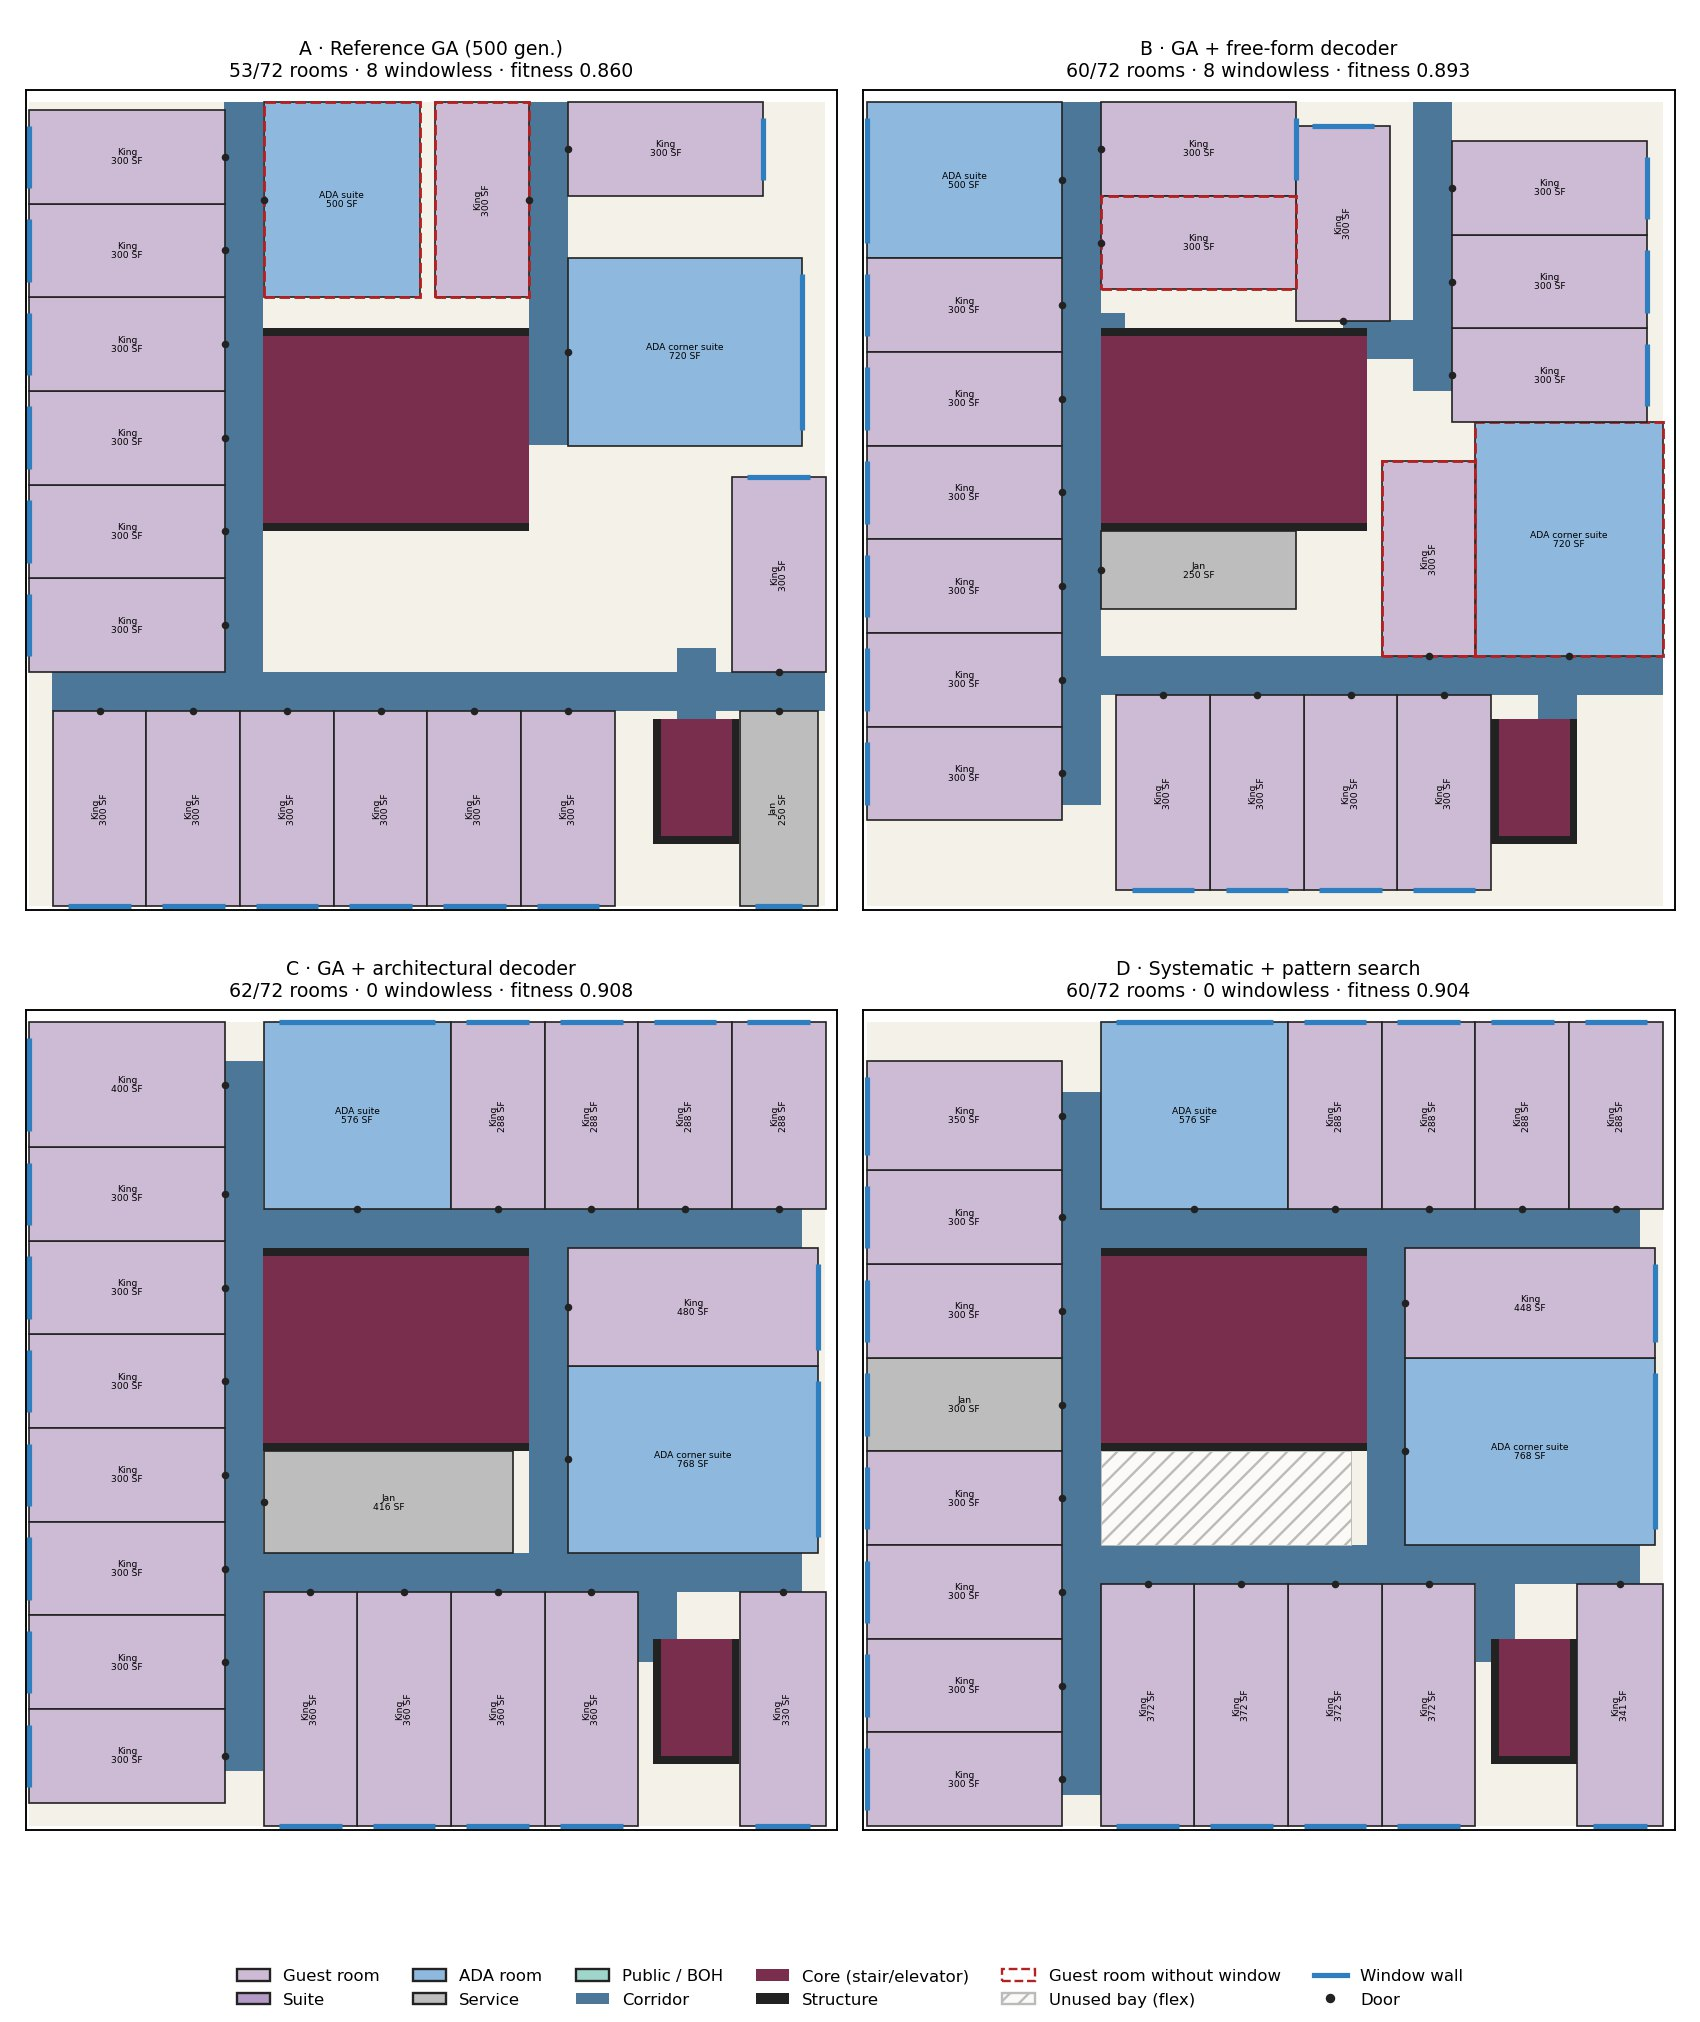
\includegraphics[width=\linewidth,keepaspectratio,height=0.80\textheight]{figures/opt_compare_fp2.jpg}\caption{Site fp2, Level 2, same program and same evaluator. Blue lines are window walls; a red dashed outline marks a guest room with no window; hatched bays are unused.}\end{figure}
\begin{figure}[H]\centering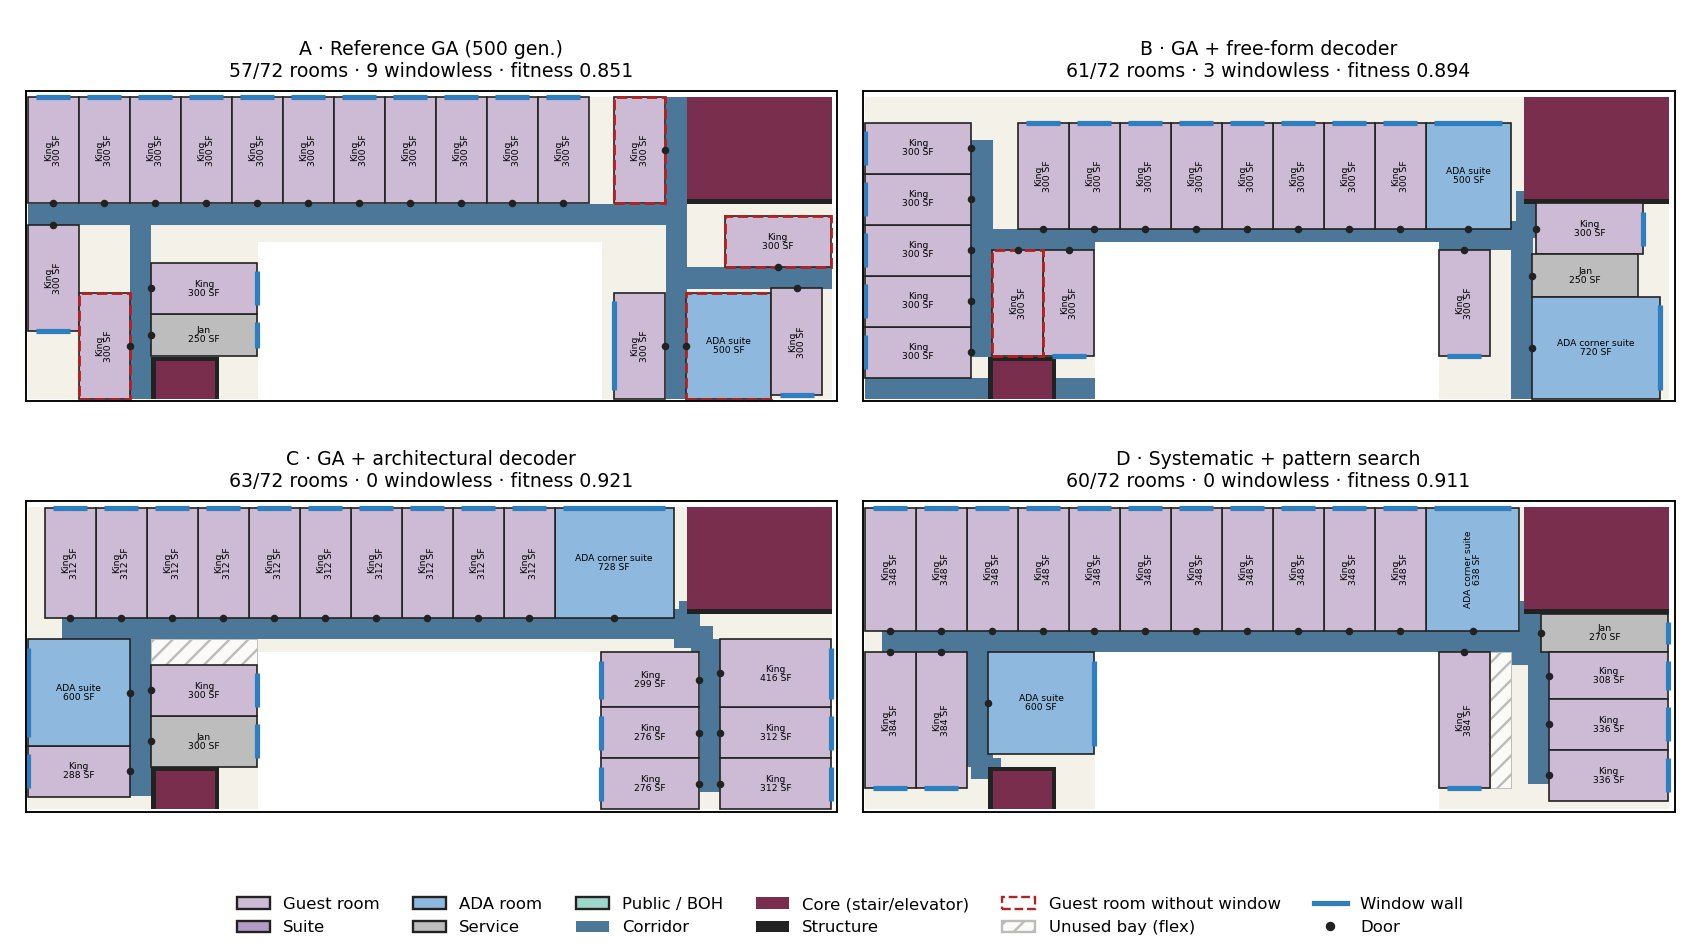
\includegraphics[width=\linewidth,keepaspectratio,height=0.80\textheight]{figures/opt_compare_fp3.jpg}\caption{Site fp3, Level 2, same program and same evaluator. Blue lines are window walls; a red dashed outline marks a guest room with no window; hatched bays are unused.}\end{figure}

\subsection{Results in Hotel Schematic (generative shape, core and floors)}\label{sec:opthotel}
Input: the Project Renegade Living + Lodging program (117 keys) and a buildable area of
170 x 265 ft. The search screened 158 plate and floor-count variants,
evaluated 1,140 layouts and kept 740 distinct ones in 36 s on eight
processes, with no LLM calls; a second run returned the same list: yes.
212 layouts are on the Pareto front. Pattern search improved the screened plates as follows:
Courtyard 156x156 $\cdot$ center core (5 fl.) 0.870 $\to$ 0.870; L 202x121 $\cdot$ ends core (5 fl.) 0.863 $\to$ 0.881; Bar 265x58 $\cdot$ center core (5 fl.) 0.863 $\to$ 0.863; T 202x121 $\cdot$ center core (5 fl.) 0.856 $\to$ 0.865.
\begingroup\captionof{table}{Top ten layouts under the Balanced decision weights.}\endgroup
{\footnotesize\begin{longtable}{p{0.38cm}p{3.99cm}p{0.95cm}p{1.14cm}p{0.85cm}p{0.76cm}p{0.95cm}p{1.04cm}p{0.85cm}p{0.85cm}p{0.95cm}p{0.76cm}}
\toprule
\textbf{\#} & \textbf{Layout} & \textbf{Guest floors} & \textbf{TOPSIS $C_j$} & \textbf{Pareto} & \textbf{Keys} & \textbf{Fitness} & \textbf{Corridor} & \textbf{SF / key} & \textbf{Height ft} & \textbf{Dead end ft} & \textbf{Code} \\ \midrule \endhead
1 & Bar 265x58 $\cdot$ center core & 4 & 0.917 & yes & 117 & 0.859 & 0.112 & 657 & 59 & 24 & 1.00 \\
2 & L 220x132 $\cdot$ knuckle core & 4 & 0.906 & yes & 117 & 0.849 & 0.120 & 729 & 59 & 26 & 1.00 \\
3 & L 170x176 $\cdot$ knuckle core & 4 & 0.905 & yes & 117 & 0.835 & 0.120 & 714 & 59 & 24 & 1.00 \\
4 & Bar 265x58 $\cdot$ ends core & 4 & 0.904 & yes & 117 & 0.845 & 0.113 & 657 & 59 & 30 & 1.00 \\
5 & Bar 265x58 $\cdot$ ends core & 4 & 0.903 & yes & 117 & 0.843 & 0.113 & 657 & 59 & 30 & 1.00 \\
6 & Bar 265x58 $\cdot$ ends core & 4 & 0.903 & yes & 117 & 0.842 & 0.113 & 657 & 59 & 31 & 1.00 \\
7 & Courtyard 156x156 $\cdot$ ends core & 4 & 0.902 & yes & 117 & 0.845 & 0.111 & 972 & 59 & 28 & 1.00 \\
8 & T 170x176 $\cdot$ knuckle core & 4 & 0.899 & no & 114 & 0.840 & 0.122 & 733 & 59 & 24 & 1.00 \\
9 & T 170x176 $\cdot$ knuckle core & 4 & 0.899 & no & 114 & 0.840 & 0.122 & 733 & 59 & 24 & 1.00 \\
10 & Bar 265x58 $\cdot$ center core & 5 & 0.897 & yes & 117 & 0.863 & 0.112 & 788 & 70 & 24 & 0.86 \\
\bottomrule
\end{longtable}}\addtocounter{table}{-1}
\begingroup\captionof{table}{Best layout of each shape (Balanced weights).}\endgroup
{\footnotesize\begin{longtable}{p{1.61cm}p{4.37cm}p{1.04cm}p{1.14cm}p{0.85cm}p{1.04cm}p{1.33cm}p{1.14cm}p{0.85cm}}
\toprule
\textbf{Shape} & \textbf{Best layout of that shape} & \textbf{Guest floors} & \textbf{Overall rank} & \textbf{Keys} & \textbf{SF / key} & \textbf{Facade ft / key} & \textbf{Dead end ft} & \textbf{Code} \\ \midrule \endhead
Bar & Bar 265x58 $\cdot$ center core & 4 & 1 & 117 & 657 & 27.6 & 24 & 1.00 \\
L & L 220x132 $\cdot$ knuckle core & 4 & 2 & 117 & 729 & 30.1 & 26 & 1.00 \\
Courtyard & Courtyard 156x156 $\cdot$ ends core & 4 & 7 & 117 & 972 & 33.5 & 28 & 1.00 \\
T & T 170x176 $\cdot$ knuckle core & 4 & 8 & 114 & 733 & 30.4 & 24 & 1.00 \\
U & U 187x112 $\cdot$ center core & 4 & 34 & 111 & 771 & 31.8 & 29 & 1.00 \\
H & H 156x136 $\cdot$ knuckle core & 4 & 206 & 106 & 854 & 34.9 & 59 & 0.86 \\
\bottomrule
\end{longtable}}\addtocounter{table}{-1}
\begingroup\captionof{table}{The first-ranked layout changes with the decision priority: the trade-off is the user's, the search only supplies the options.}\endgroup
{\footnotesize\begin{longtable}{p{2.66cm}p{4.94cm}p{1.23cm}p{0.95cm}p{1.14cm}p{1.23cm}p{0.95cm}}
\toprule
\textbf{Decision priority} & \textbf{Layout ranked first} & \textbf{Guest floors} & \textbf{Keys} & \textbf{SF / key} & \textbf{Height ft} & \textbf{Code} \\ \midrule \endhead
Balanced & Bar 265x58 $\cdot$ center core & 4 & 117 & 657 & 59 & 1.00 \\
Most keys & Courtyard 156x156 $\cdot$ center core & 4 & 117 & 972 & 59 & 1.00 \\
Lowest cost & Bar 265x58 $\cdot$ center core & 4 & 117 & 657 & 59 & 1.00 \\
Guest experience & Bar 265x58 $\cdot$ center core & 4 & 117 & 657 & 59 & 1.00 \\
Low-rise & Bar 265x58 $\cdot$ center core & 4 & 117 & 657 & 59 & 1.00 \\
\bottomrule
\end{longtable}}\addtocounter{table}{-1}
\textbf{First-ranked layout: Bar 265x58 $\cdot$ center core, 4 guest floors.} Footprint 265 x 58 ft
(15,370 SF), 2 elevators, bay module 13 ft. It places
117 of 117 keys and 142 of 150 program rooms; the
frontage bound is 34 keys per typical floor. Corridor share 0.112, longest exit
travel 64 ft, dead end 24 ft, fitness 0.859. Not placed: White Box Retail x1, IT x1, Jan x2, Gym x1, MEP Service x1, Loading x1, Luggage x1.
{\footnotesize\begin{longtable}{p{1.80cm}p{4.37cm}p{4.37cm}p{2.28cm}p{1.23cm}}
\toprule
\textbf{Rule} & \textbf{Check} & \textbf{Required} & \textbf{Provided} & \textbf{Status} \\ \midrule \endhead
IBC-R1-015 & Exits per story (cores reached) & $\ge$ 2 & 3 & \textcolor{pass}{\textbf{PASS}} \\
IBC-R1-018 & Exit separation (core to core) & $\ge$ 1/3 diagonal = 90 ft & 202 ft & \textcolor{pass}{\textbf{PASS}} \\
IBC-R1-023 & Exit access travel & $\le$ 250 ft & 63 ft & \textcolor{pass}{\textbf{PASS}} \\
IBC-R1-025 & Corridor width & $\ge$ 44 in & 72 in & \textcolor{pass}{\textbf{PASS}} \\
IBC-R1-027 & Dead-end corridor & $\le$ 50 ft & 24 ft & \textcolor{pass}{\textbf{PASS}} \\
ADA-224.2 & ADA mobility rooms & $\ge$ 7 for 117 keys & 7 & \textcolor{pass}{\textbf{PASS}} \\
IBC-R1-007 & Stories above grade & $\le$ 5 (Type IIA, sprinklered R-1) & 5 & \textcolor{pass}{\textbf{PASS}} \\
\bottomrule
\end{longtable}}\addtocounter{table}{-1}
\begin{figure}[H]\centering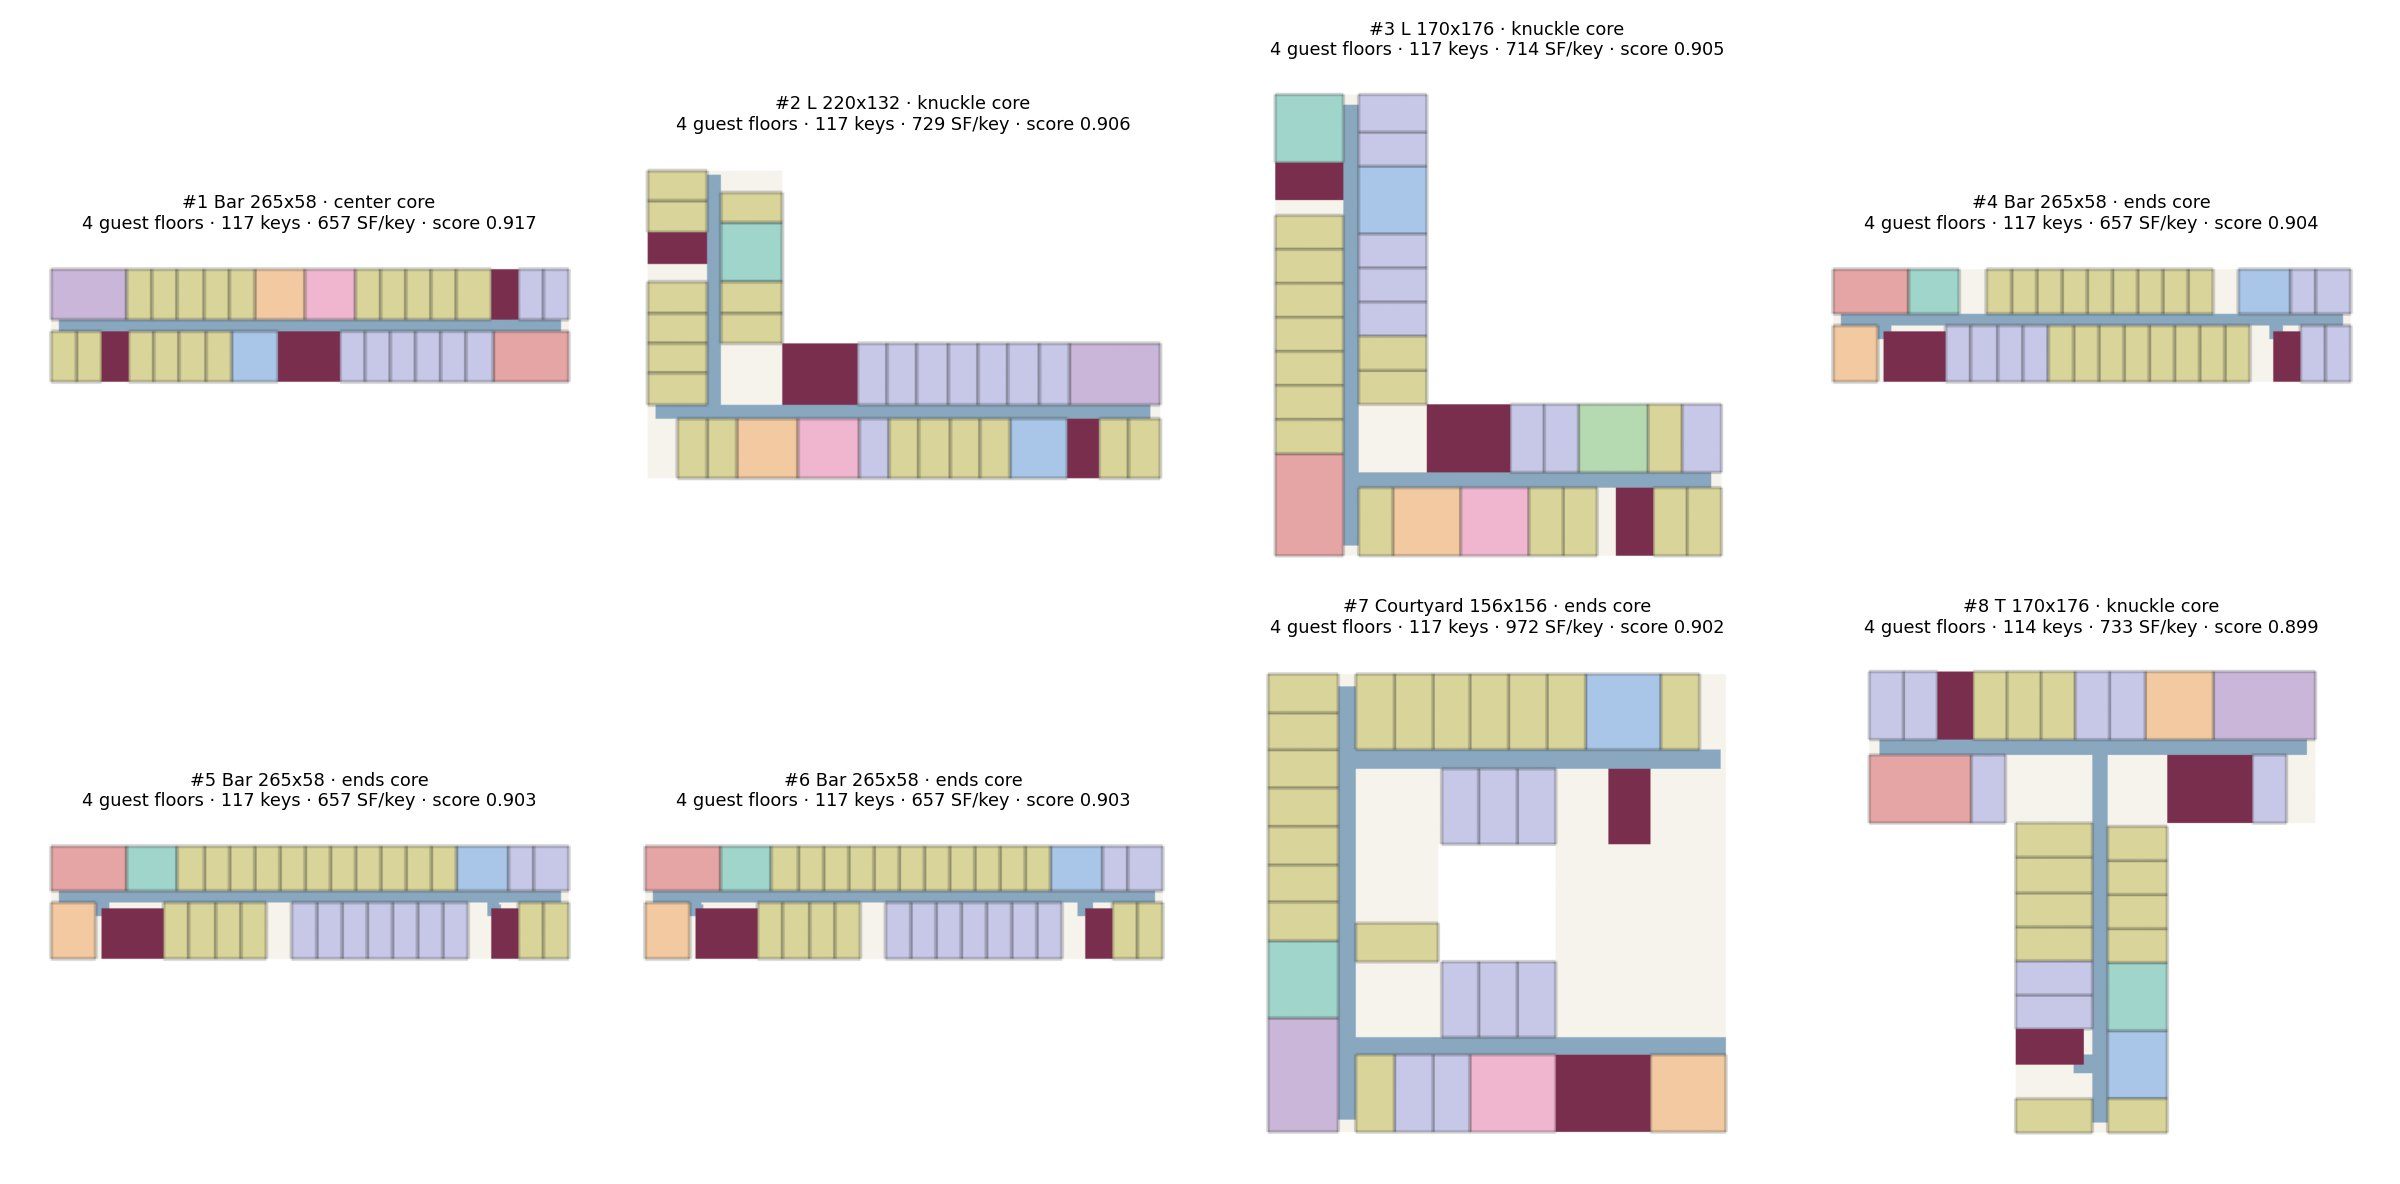
\includegraphics[width=\linewidth,keepaspectratio,height=0.45\textheight]{figures/opt_hotel_gallery.jpg}\caption{The eight first-ranked layouts (typical guest floor). Dark red: core and stairs; blue: corridor.}\end{figure}
\begin{figure}[H]\centering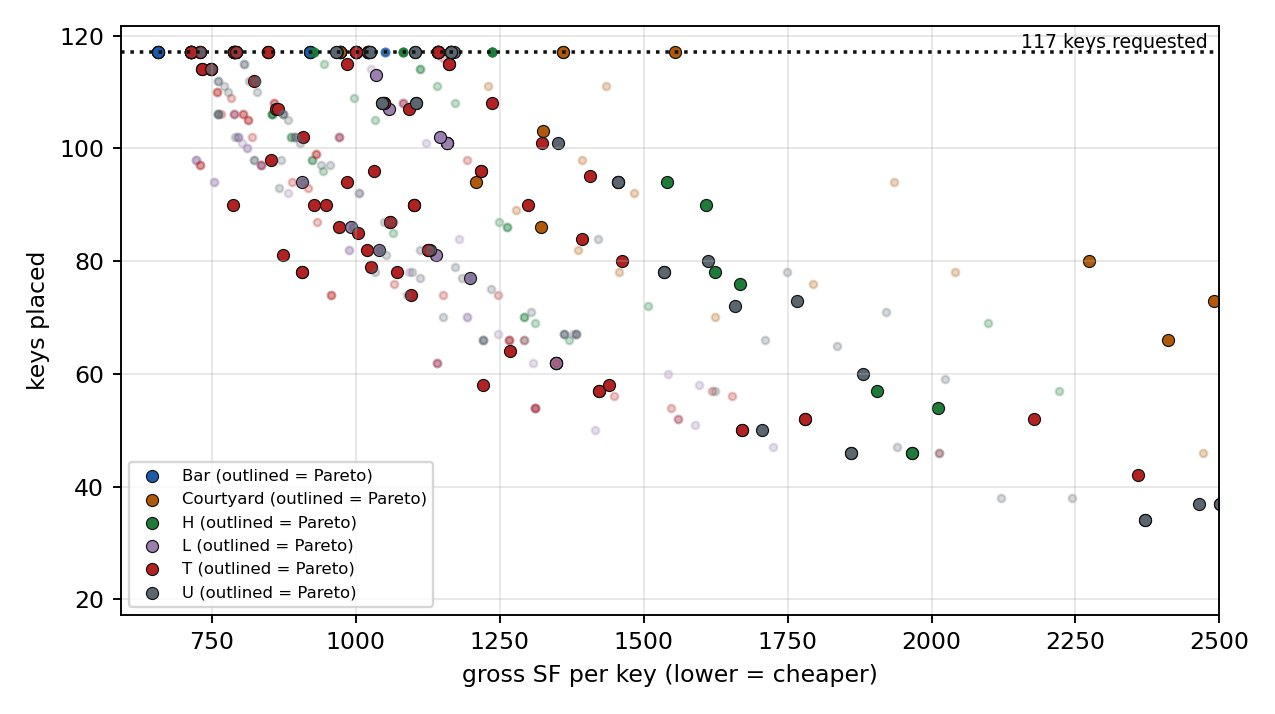
\includegraphics[width=\linewidth,keepaspectratio,height=0.34\textheight]{figures/opt_hotel_pareto.jpg}\caption{Every layout found: keys placed against gross area per key. Outlined points are on the Pareto front.}\end{figure}
\begin{figure}[H]\centering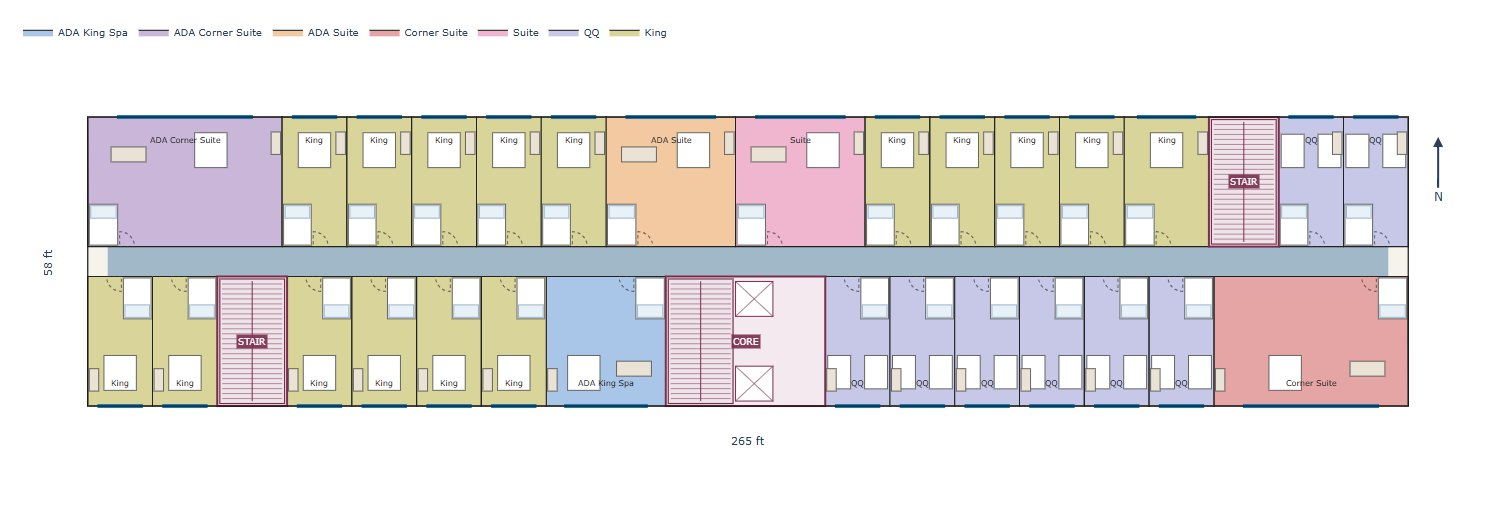
\includegraphics[width=\linewidth,keepaspectratio,height=0.40\textheight]{figures/opt_hotel_best_L2.jpg}\caption{First-ranked layout, Level 2, as drawn in the app: furnished rooms, door swings, windows (blue), stairs and elevators.}\end{figure}
\begin{figure}[H]\centering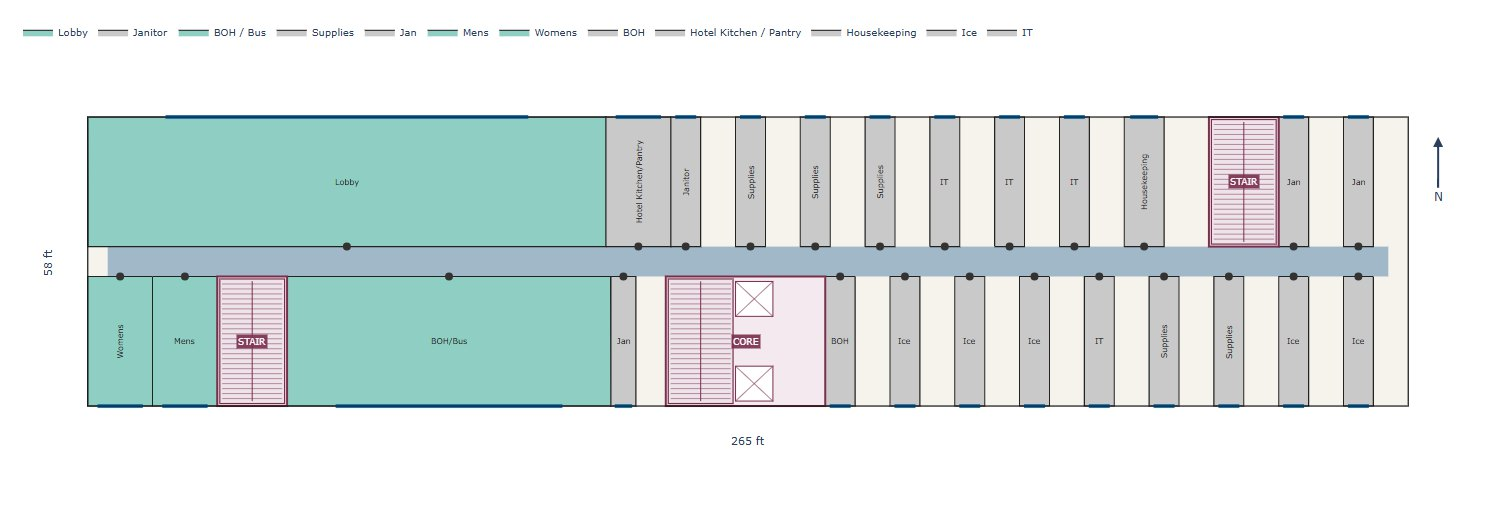
\includegraphics[width=\linewidth,keepaspectratio,height=0.40\textheight]{figures/opt_hotel_best_L1.jpg}\caption{First-ranked layout, Level 1 (public and back-of-house rooms).}\end{figure}
\begin{figure}[H]\centering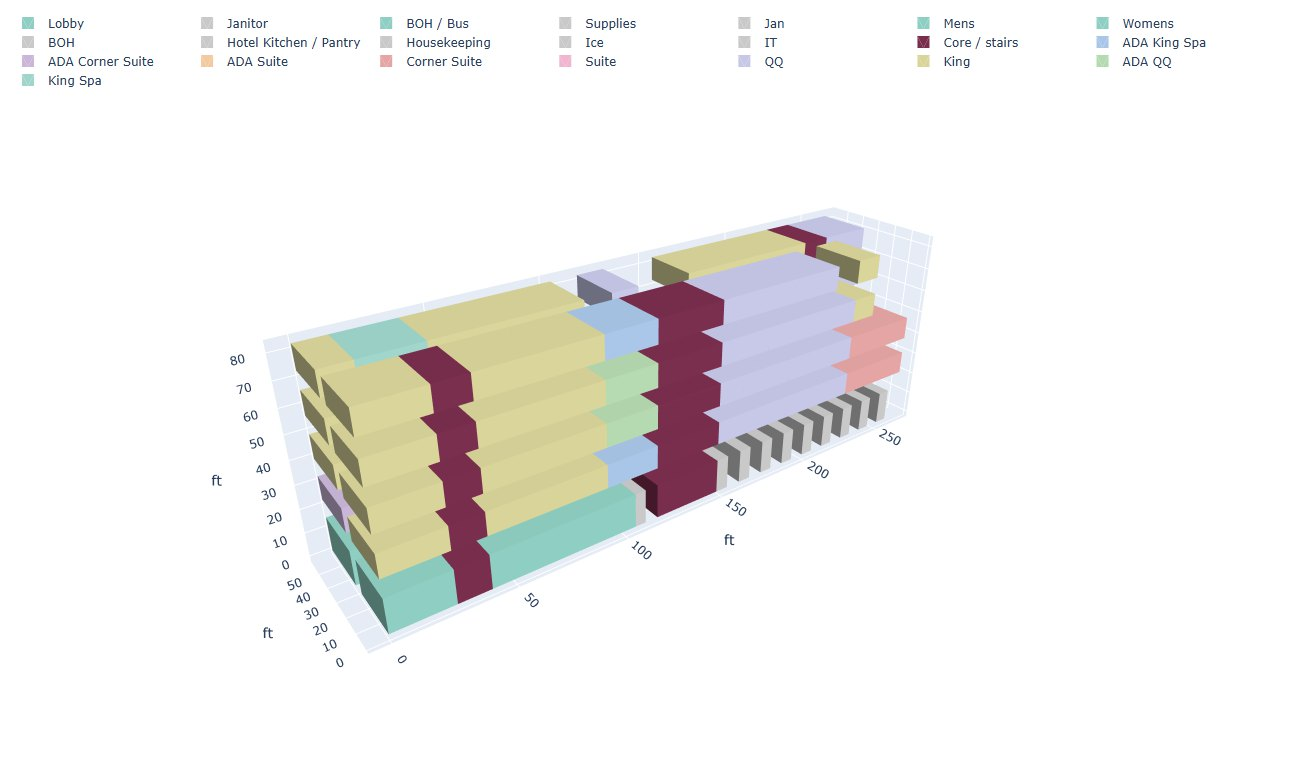
\includegraphics[width=\linewidth,keepaspectratio,height=0.38\textheight]{figures/opt_hotel_best_3d.jpg}\caption{First-ranked layout, stacked massing with the floors pulled apart.}\end{figure}

\subsection{App screenshots}
\begin{figure}[H]\centering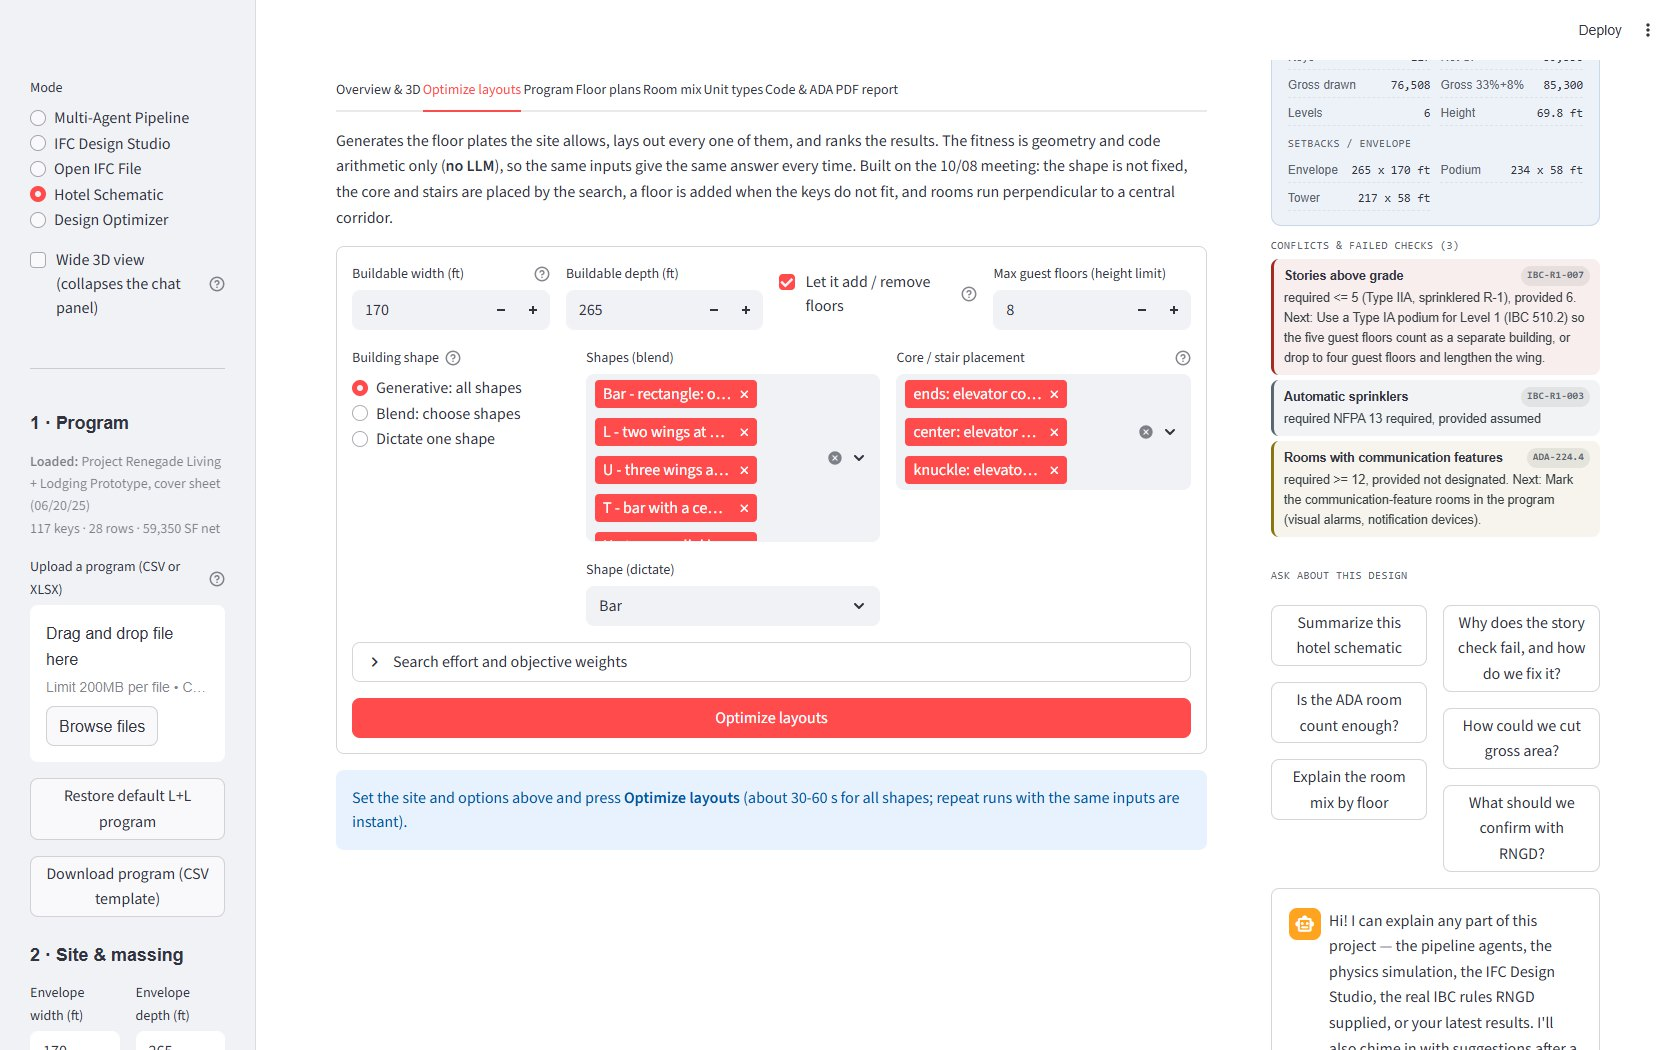
\includegraphics[width=\linewidth,keepaspectratio,height=0.42\textheight]{figures/snap_32_hotel_optimize_settings.jpg}\caption{Optimize layouts: buildable area, shape mode (generative, blend or one shape), core placement and floors.}\end{figure}
\begin{figure}[H]\centering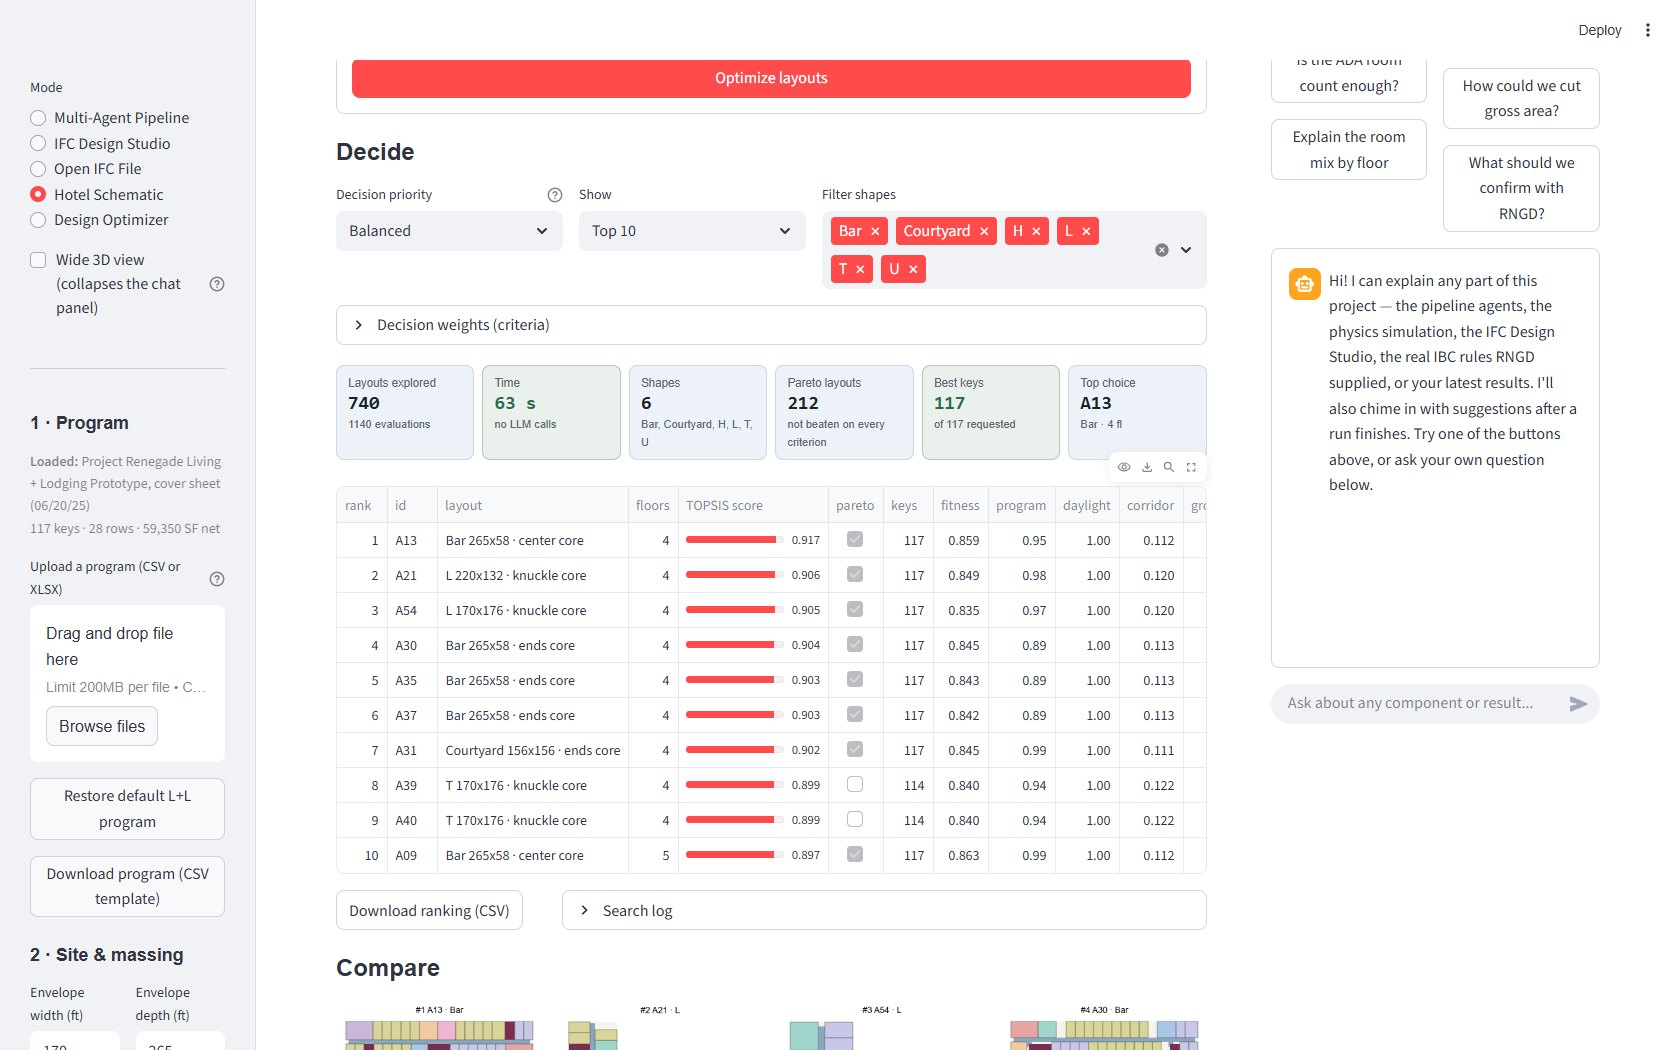
\includegraphics[width=\linewidth,keepaspectratio,height=0.42\textheight]{figures/snap_33_hotel_optimize_decide.jpg}\caption{Decision step: every distinct layout ranked by TOPSIS under the chosen priority, with the Pareto flag; the Show dropdown switches between the top 5, 10 or 25, the Pareto front and all layouts.}\end{figure}
\begin{figure}[H]\centering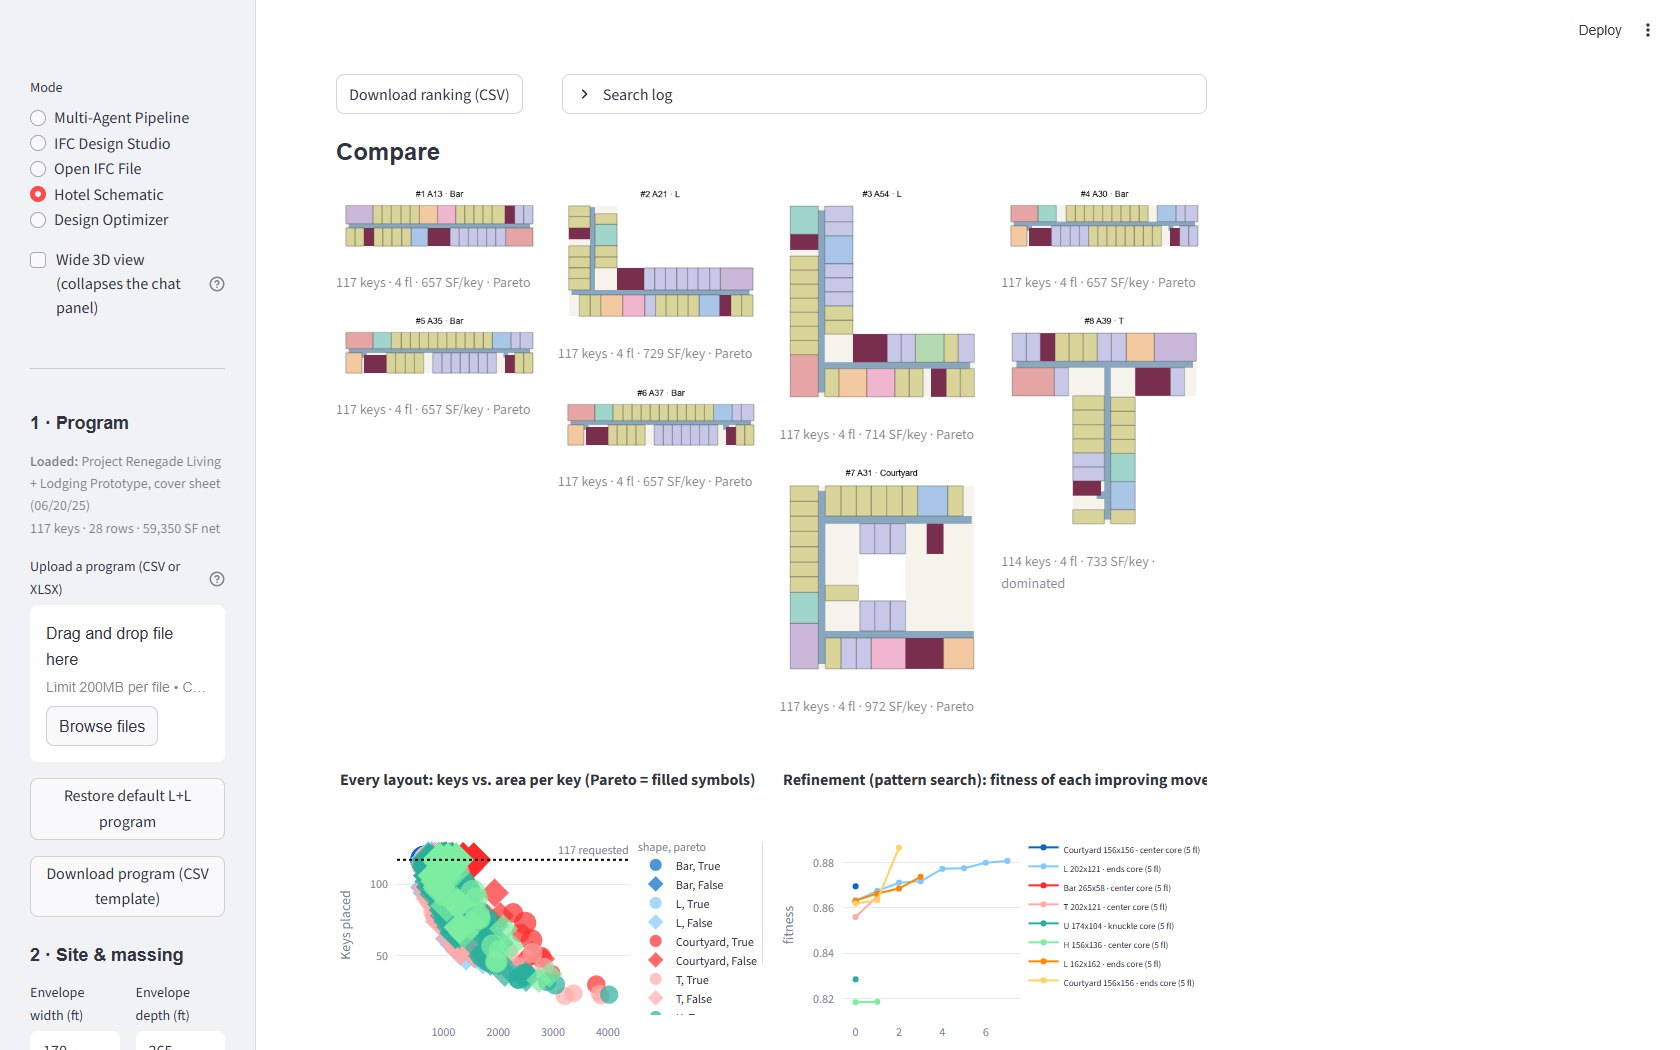
\includegraphics[width=\linewidth,keepaspectratio,height=0.42\textheight]{figures/snap_34_hotel_optimize_compare.jpg}\caption{Comparison: typical-floor thumbnails of the first-ranked layouts, keys against gross area per key for every layout, and the fitness gained by pattern search.}\end{figure}
\begin{figure}[H]\centering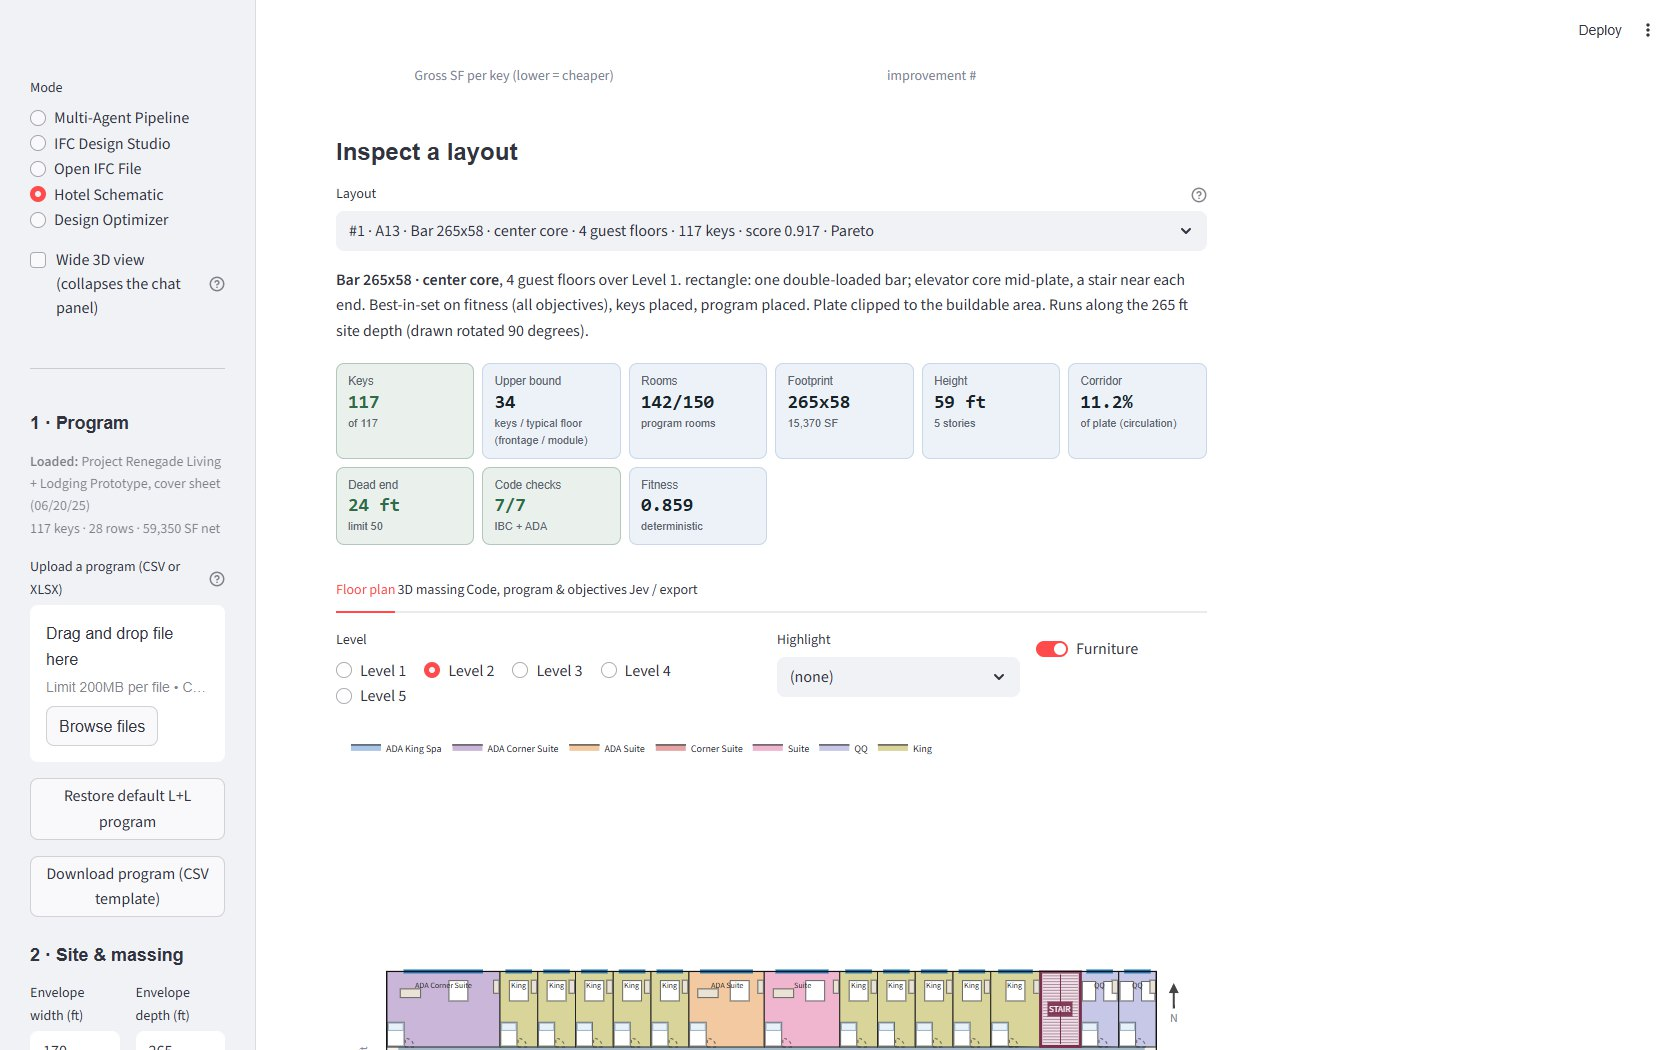
\includegraphics[width=\linewidth,keepaspectratio,height=0.42\textheight]{figures/snap_35_hotel_optimize_inspect.jpg}\caption{One layout inspected: keys, upper bound, footprint, corridor share, dead end, code checks and fitness.}\end{figure}
\begin{figure}[H]\centering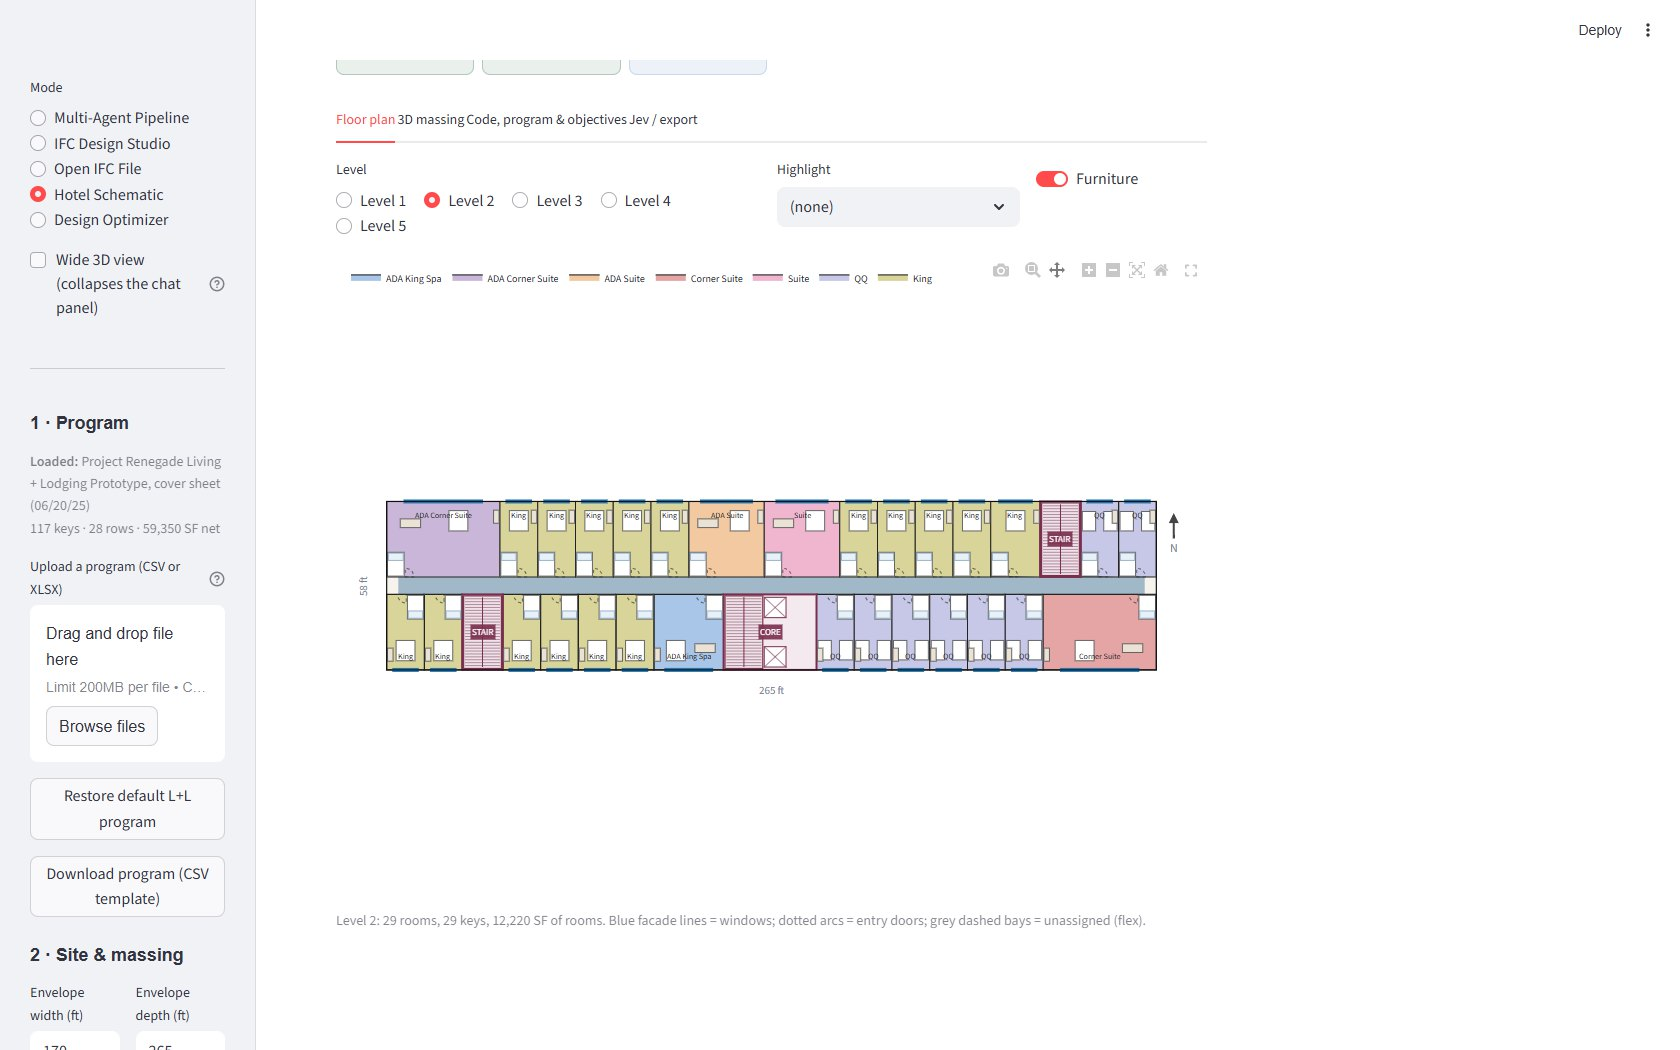
\includegraphics[width=\linewidth,keepaspectratio,height=0.42\textheight]{figures/snap_36_hotel_optimize_plan.jpg}\caption{Interactive furnished plan of the selected layout (hover gives room data).}\end{figure}
\begin{figure}[H]\centering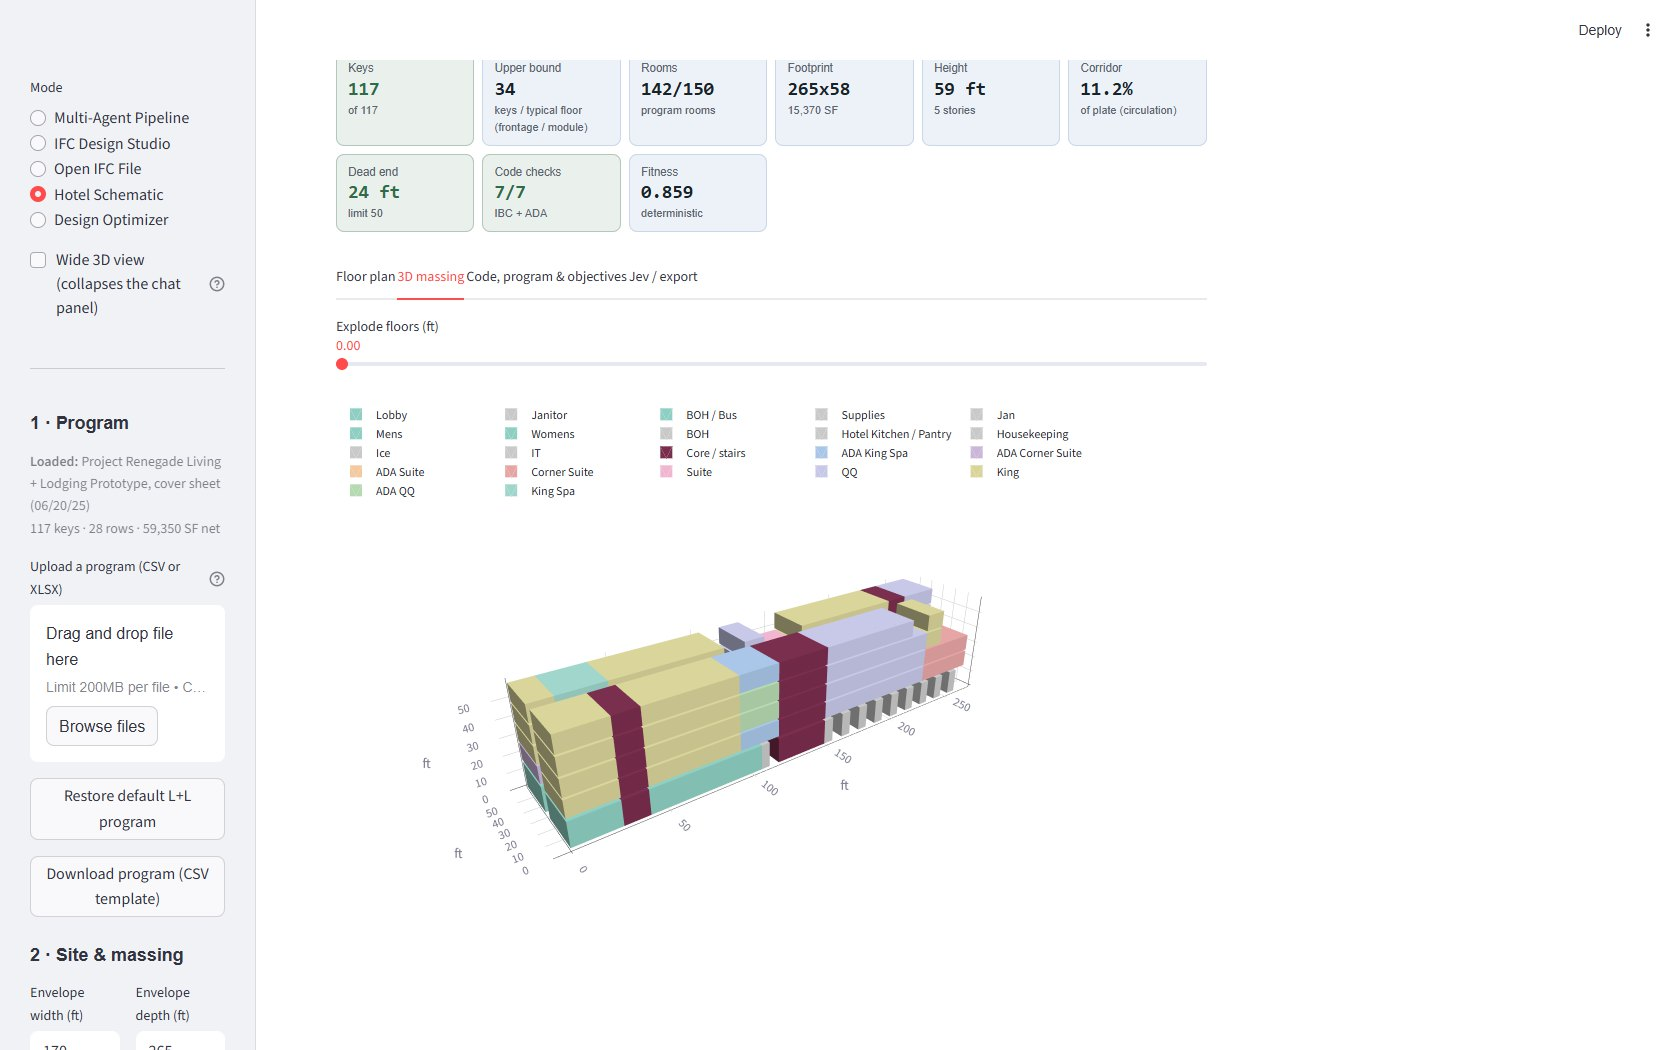
\includegraphics[width=\linewidth,keepaspectratio,height=0.42\textheight]{figures/snap_37_hotel_optimize_3d.jpg}\caption{Stacked 3D massing of the selected layout, coloured by room type.}\end{figure}

\subsection{What is still open}
\begin{itemize}
\item Level 1 uses the same plate as the guest floors (no wider podium), so large ground-floor rooms can be left out; they are listed for every layout.
\item The decoder draws rectangles on a 1 ft grid: angled wings, curved facades and structural grids are not modelled.
\item The upper bounds are loose; a tight bound would need an exact packing model.
\item The centre-core scheme uses two stairs; on T, U and H plates the third wing can exceed the dead-end limit. The check flags it and the ranking moves such layouts down.
\item Parking, cost and energy are not in the fitness. Facade length per key and gross area per key stand in for cost in the decision step.
\item Jev (TypeSafe's hosted decision model) is wired only as an optional advisor; no key was configured for this run.
\end{itemize}

\endgroup

\subsection{Relation to known methods}
The reference prototype and variants B and C are genetic algorithms~\citep{holland1975adaptation,goldberg1989genetic}:
a population of encoded plans is improved by selection, crossover and mutation. Variant C adds a local-search step to
each generation, which makes it a memetic algorithm~\citep{moscato1989memetic}. The room-order part of the genome is a
random-key encoding~\citep{bean1994randomkeys}: one real number per room, sorted to give the order in which rooms claim
bays, so any vector of numbers decodes to a valid order. The systematic search (variant D) combines exhaustive
enumeration of a small structured space with a first-improvement pattern search in the spirit of Hooke and
Jeeves~\citep{hooke1961direct}, and then iterated local search~\citep{lourenco2003ils}. The decision step keeps the
non-dominated layouts~\citep{deb2001multi} and ranks them with TOPSIS~\citep{hwang1981topsis}. The main change from the
reference is the encoding rather than the search method: the search no longer moves corridor segments and rooms
directly, it chooses among corridors that already make architectural sense.

% =====================================================================
\clearpage
\section{Implementation: the most important code}
\label{sec:code}

The listings below are extracted verbatim from the repository by \code{src/build\_paper.py}; each starts with its source
path.

\subsection{Model access with a provider guard and JSON repair}
Every LLM call goes through \code{call\_json}. It refuses blocked model families, asks for JSON, and feeds a parsing
error back to the model for a retry. This is the first guardrail against malformed or invented output.
\lstinputlisting{code/llm_guard.py}

\subsection{An agent prompt and its schema}
The intake agent's instructions define the exact keys to return and tell the model to mark a requirement as hard only
when the text says so; the output is validated by pydantic.
\lstinputlisting{code/intake_prompt.py}

\subsection{Arithmetic stays in Python}
The envelope, module counts and feasibility numbers (\cref{sec:pipeline}) are plain functions. Their results are
\emph{inputs} to the LLM prompts, never outputs of them.
\lstinputlisting{code/envelope.py}
\lstinputlisting{code/modules.py}
\lstinputlisting{code/feasibility.py}

\subsection{Retrieval}
\lstinputlisting{code/retrieval.py}

\subsection{Physics engine}
The separation force acts along the axis of least overlap. The sign was a real bug: an early version pushed bodies
together and diverged. \code{step} integrates with damping, and \code{run} stops on convergence.
\lstinputlisting{code/physics.py}

\subsection{Vision calibration and the critic loop}
\lstinputlisting{code/calibration.py}
The loop exit is decided by code; the critic only proposes deltas, which are clamped.
\lstinputlisting{code/loop.py}
\lstinputlisting{code/critic.py}

\subsection{Real IFC recentring}
\lstinputlisting{code/recenter.py}

\subsection{Hotel generator}
Routing the program rows, balancing the wing (\cref{alg:wing}), and the egress geometry used by the code screen:
\lstinputlisting{code/split_rows.py}
\lstinputlisting{code/hotel_wing.py}
\lstinputlisting{code/hotel_egress.py}
The code screen evaluates RNGD's rules from the geometry, and the ADA table is encoded exactly:
\lstinputlisting{code/code_check.py}
\lstinputlisting{code/ada.py}
Placing a room and projecting to 3D:
\lstinputlisting{code/transform.py}

\subsection{Layout optimizer}
The fitness (\cref{sec:optmath}) is a weighted mean of cached objective terms minus the penalty for an exit the
corridor does not reach. It contains no model call:
\lstinputlisting{code/opt_fitness.py}
Stage 1 of the systematic search builds one genome per set of corridor spines, with every room-order key at 0.5 so
that rooms claim bays in priority order:
\lstinputlisting{code/opt_enumerate.py}
For the hotel, the elevator count and the corridor length each plate shape offers:
\lstinputlisting{code/opt_plate.py}
The decision step, Pareto dominance and TOPSIS:
\lstinputlisting{code/opt_decide.py}

% =====================================================================
\section{Evaluation: dynamic or hallucinating?}
\label{sec:eval}

\subsection{The hotel generator responds to inputs and repeats exactly}
Four inputs were each built twice. The fingerprint is a SHA-256 of every room's position and size plus every check
result.

\begin{table}[H]
\centering\scriptsize
\caption{Four inputs to the hotel generator.}
\label{tab:hotelcases}
\resizebox{\linewidth}{!}{%
\begin{tabular}{@{}l r r l r r r c l l c@{}}
\toprule
\textbf{Case} & \textbf{Keys} & \textbf{Lvls} & \textbf{Keys/floor} & \textbf{Wing} & \textbf{L1} & \textbf{Gross SF} & \textbf{ADA req$\to$prov} & \textbf{Fails} & \textbf{Hash} & \textbf{Same?} \\ \midrule
A1 L+L, 5 floors & 117 & 6 & 24,24,23,23,23 & 217.0 & 234.1 & 76,508 & 7$\to$7 & stories & f1ecee4c & yes \\
A2 L+L, 4 floors & 117 & 5 & 30,29,29,29 & 258.0 & 258.0 & 74,828 & 7$\to$7 & none & 7b58316d & yes \\
A3 76-key program & 76 & 5 & 19,19,19,19 & 167.5 & 167.5 & 48,564 & 5$\to$4 & ADA rooms & ff6fff58 & yes \\
A4 scaled to 161 keys & 161 & 6 & 33,32,32,32,32 & 288.4 & 288.4 & 100,359 & 8$\to$10 & stories, envelope & b4fea144 & yes \\
\bottomrule
\end{tabular}}
\end{table}

\begin{itemize}
\item \textbf{Geometry follows the input.} Fewer floors give a longer wing; a smaller program gives a shorter wing; a
larger program overflows the 265\,ft envelope.
\item \textbf{Checks follow the input.}
  \begin{itemize}
  \item A2 passes the story limit (Level~1 plus four floors makes five stories).
  \item A3 fails ADA because 76 rooms need 5 accessible rooms and the program has 4.
  \item A4 does not fit the lot.
  \end{itemize}
\item \textbf{Identical inputs give identical outputs}, room for room.
\end{itemize}

\begin{figure}[H]
\centering
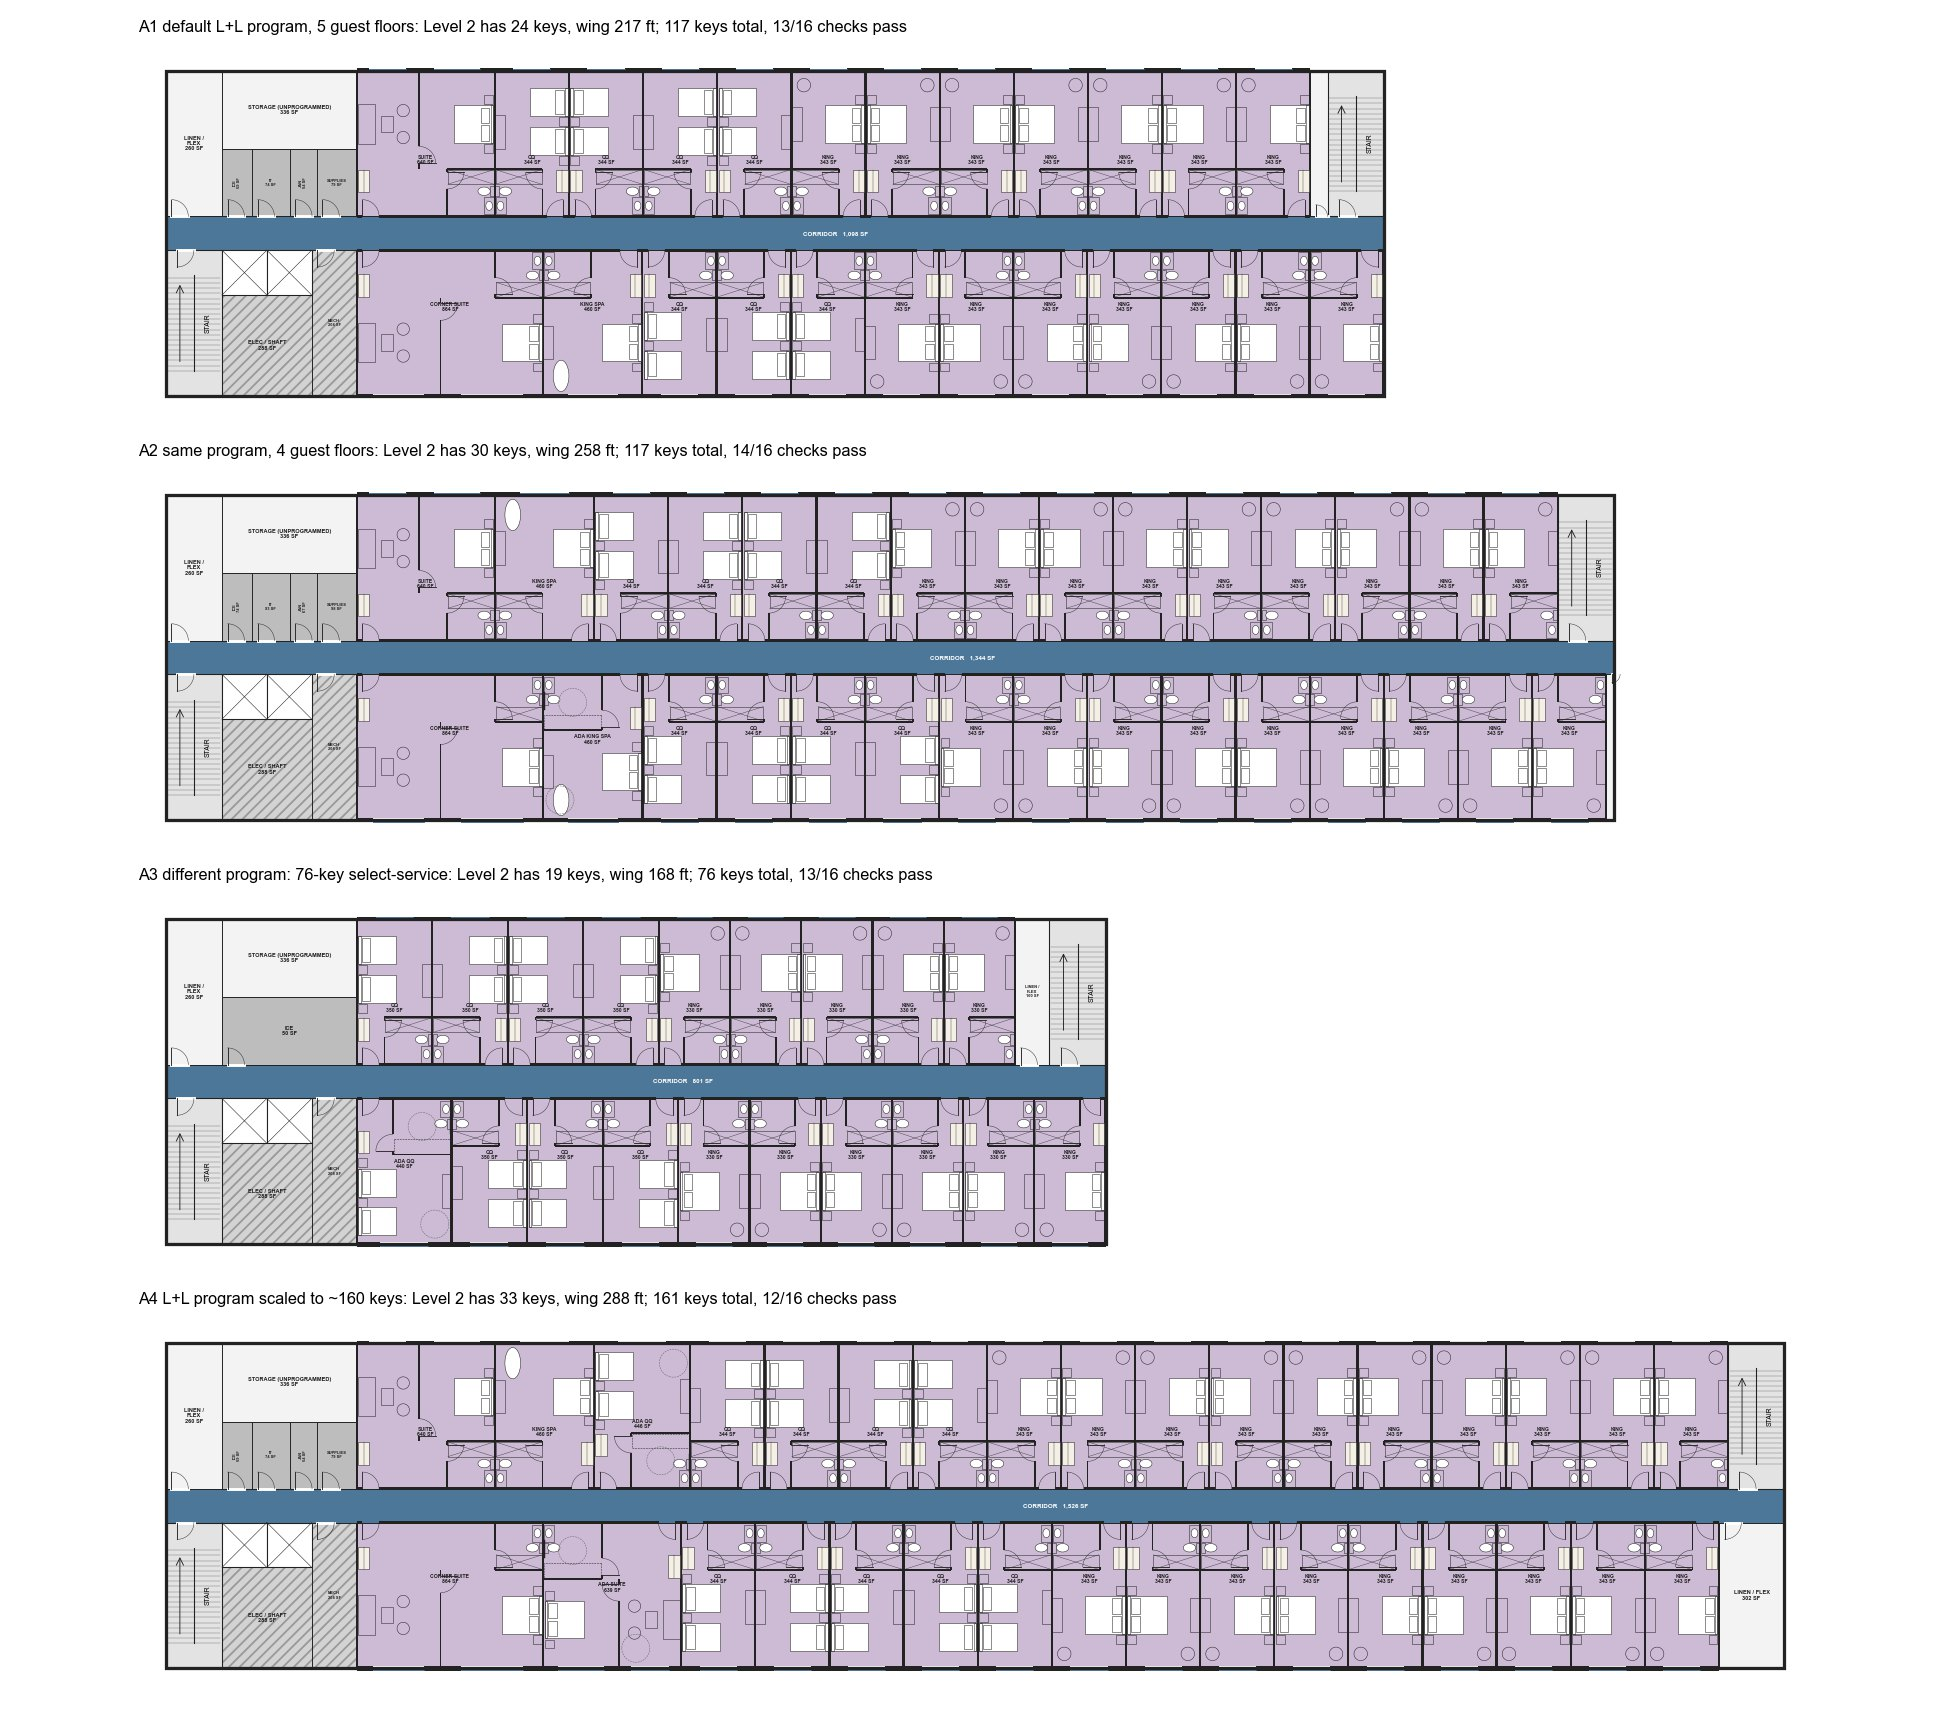
\includegraphics[width=\linewidth]{figures/fig_hotel_inputs_level2.jpg}
\caption{Level 2 of cases A1--A4 at the same scale.}
\end{figure}
\begin{figure}[H]
\centering
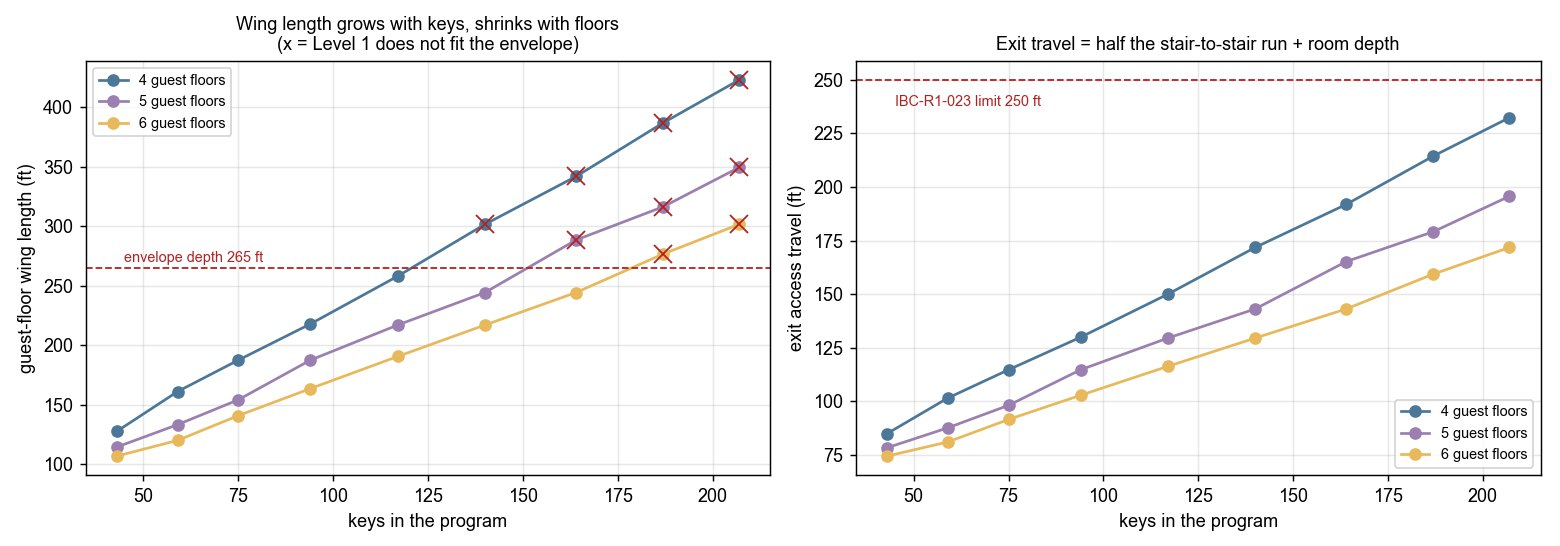
\includegraphics[width=\linewidth]{figures/fig_hotel_sweep.jpg}
\caption{Sweep from 43 to 207 keys at 4, 5 and 6 guest floors. Wing length grows with keys and shrinks with floors
($\times$ marks cases where Level 1 does not fit the envelope). Exit travel follows $T=(L-10)/2+26$ and stays below
250\,ft.}
\end{figure}

\subsection{The layout optimizer improves on the reference and repeats exactly}
\label{sec:evalopt}
The reference GA's delivered designs and three later variants were scored by one evaluator on the prototype's three
sites, with the same 72-room program per site (\cref{tab:optcompare}; budget \optBudget{} evaluations for B, C and D,
seed 7, no LLM).

\begin{table}[H]
\centering\small
\caption{Totals over the three sites (\optRoomsTotal{} rooms asked): rooms placed, guest rooms without a window, mean fitness and run time for all three sites. Run time was not recorded for the reference; its
history holds \optGensA{} generations.}
\label{tab:optsummary}
\begin{tabular}{@{}l r r r r@{}}
\toprule
\textbf{Variant} & \textbf{Rooms} & \textbf{No window} & \textbf{Fitness} & \textbf{Time} \\ \midrule
A reference GA & \optRoomsA & \optNoWinA & \optFitA & n/a \\
B GA, free-form corridors (first attempt) & \optRoomsB & \optNoWinB & \optFitB & \optSecsB\,s \\
C updated GA, architectural decoder & \optRoomsC & \optNoWinC & \optFitC & \optSecsC\,s \\
D systematic search, same decoder (default) & \optRoomsD & \optNoWinD & \optFitD & \optSecsD\,s \\
\bottomrule
\end{tabular}
\end{table}

\begin{itemize}
\item \textbf{The decoder gives the gain.} B keeps the reference representation with better scoring and does not
remove the windowless rooms. C and D share the new decoder and both do.
\item \textbf{The search method matters less.} At the same budget the GA (C) scores slightly above the systematic
search (D). D is the default because it needs no population or crossover and returns the same layout on every run,
which was checked by running it twice on each site.
\item \textbf{The comparison uses one measure.} The dead-end measure was corrected during this work (distance to the
nearest exit door or through-route) and is applied to the reference designs as well.
\item \textbf{Hotel mode.} The exploration of the Living\,+\,Lodging program kept \optHotelLayouts{} distinct layouts
from \optHotelVariants{} plate and floor-count variants in \optHotelSecs\,s, and a second run returned the same list.
The first-ranked layout (\optHotelBest, \optHotelFloors{} guest floors) places \optHotelKeys{} of \optHotelKeysAsked{}
keys and passes \optHotelChecks{} checks, but only \optHotelRooms{} of \optHotelRoomsTotal{} program rooms: some
Level~1 rooms do not fit a plate sized for the guest floors.
\end{itemize}

\subsection{The LLM agents extract what the documents say}

\begin{table}[H]
\centering\small
\caption{Intake agent on the original and an edited request.}
\begin{tabular}{@{}l c c c c l@{}}
\toprule
\textbf{Input} & \textbf{Units} & \textbf{Floors} & \textbf{Mix} & \textbf{Budget} & \textbf{Hard requirements} \\ \midrule
original, run 1 & 120 & 4 & .20/.45/.35 & \$28.0M & ``120 units'' \\
original, run 2 & 120 & 4 & .20/.45/.35 & \$28.0M & ``120 units'' \\
\textbf{edited} & \textbf{84} & \textbf{6} & \textbf{.10/.50/.40} & \textbf{\$19.5M} & ``84 units firm requirement'', ``parking per local code'' \\
\bottomrule
\end{tabular}
\end{table}

\begin{table}[H]
\centering\small
\caption{Zoning agent versus the values printed in the knowledge base (two runs).}
\begin{tabular}{@{}l c c c@{}}
\toprule
\textbf{Limit} & \textbf{Knowledge base} & \textbf{Run 1} & \textbf{Run 2} \\ \midrule
height / stories / FAR / coverage & 65\,ft / 5 / 2.5 / 60\% & same & same \\
setbacks front / side / rear & 15 / 10 / 20\,ft & same & same \\
parking ratio / fire lane & 1.25 per unit / 20\,ft & same & same \\
\textbf{all 9 limits match} & & \textbf{yes} & \textbf{yes} \\
\bottomrule
\end{tabular}
\end{table}

Every number in the saved arbiter narrative (1.25, 15, 120, 135, 150) appears in the computed data: the parking ratio,
detected stalls, units, the shortfall $150-15$, and required stalls $1.25\times120$.

\subsection{Run-to-run variability}
\label{sec:variability}
\begin{table}[H]
\centering\small
\caption{Three full pipeline runs of the same project (2026-10-05).}
\begin{tabular}{@{}l l l l@{}}
\toprule
 & \textbf{Browser run 15:55} & \textbf{Test-suite run 16:12} & \textbf{Run 17:29} \\ \midrule
Decision & REVISE (0.95) & REVISE (0.95) & REVISE (0.93) \\
Conflicts & 2 & 2 (critical, medium) & 1 (high) \\
Critic & stopped, shortfall unresolved & tried $+50\times50$\,ft, then stopped & stopped after iteration 1 \\
Stalls found by CV & 15/150 & 34/150 & 15/150 \\
\bottomrule
\end{tabular}
\end{table}

\begin{itemize}
\item \textbf{Stable across runs:} the extracted program, zoning limits, envelope, module counts, feasibility numbers,
the decision (REVISE in 3 of 3) and its reason (surface parking cannot fit).
\item \textbf{Varies across runs:} how the LLM rates conflicts, and whether the critic tries one more geometry change.
In the 16:12 run it enlarged the building; vision QA caught the resulting setback violation, and the arbiter still
returned REVISE.
\end{itemize}
Each narrative's numbers came from its own run's measurements.

\subsection{Tests and timings}
All 51 automated tests pass. They cover the pipeline agents, the IFC engine with an IFC round trip, the hotel
generator, ADA tables, interactive figures, the layout optimizer (decoder, fitness, determinism of the systematic
search, hotel exploration and ranking), and app tests that drive the real Streamlit app, including a full pipeline
run with real LLM calls. In the browser run, the pipeline took 105\,s, opening the 89\,MB IFC file 52\,s, generating
the hotel PDF 24\,s and an assistant reply 37\,s, with no on-page errors across 31 screenshots.

% =====================================================================
\section{Discussion}
\label{sec:discussion}

\subsection{Guardrails against hallucination}
\begin{figure}[H]
\centering
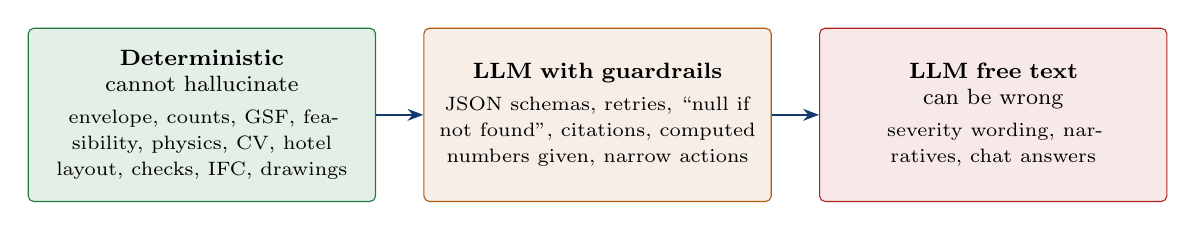
\begin{tikzpicture}[node distance=6mm]
\node[box, fill=okc!12, draw=okc, text width=42mm, minimum height=22mm] (a) {\textbf{Deterministic}\\cannot hallucinate\\[2pt]\scriptsize envelope, counts, GSF, feasibility, physics, CV, hotel layout, checks, IFC, drawings};
\node[box, fill=warnc!10, draw=warnc, text width=42mm, minimum height=22mm, right=of a] (b) {\textbf{LLM with guardrails}\\[2pt]\scriptsize JSON schemas, retries, ``null if not found'', citations, computed numbers given, narrow actions};
\node[box, fill=failc!10, draw=failc, text width=42mm, minimum height=22mm, right=of b] (c) {\textbf{LLM free text}\\can be wrong\\[2pt]\scriptsize severity wording, narratives, chat answers};
\draw[arr] (a) -- (b); \draw[arr] (b) -- (c);
\end{tikzpicture}
\caption{Where errors can and cannot come from.}
\end{figure}

The code enforces eight guardrails:
\begin{enumerate}
\item Arithmetic is never left to the model.
\item Agent outputs are validated against schemas, with retries.
\item The zoning prompt says to return \code{null} rather than invent a number, and to cite the source section.
\item Vision QA measures the drawing independently of the simulation.
\item The critic can change only three parameters, and the loop is capped in code.
\item The arbiter must not approve with an unresolved critical or high conflict.
\item The hotel and IFC designs use no LLM, and neither does the layout optimizer's fitness or search.
\item LLM requests time out after 90\,s.
\end{enumerate}
One observed error shows the remaining risk. The chat assistant explained the story-count failure with an ``8\,ft''
story definition that is not in RNGD's rules; the code check itself was right. Chat answers are explanations; the code
screens are the facts.

\subsection{Engineering lessons (bugs found and fixed)}
\begin{itemize}
\item \textbf{Physics sign error.} Separation pushed bodies together and the solver diverged. The fixed version converges in six steps.
\item \textbf{DPI mismatch.} The calibration used 100\,dpi while the PNG was 140\,dpi, a $1.4\times$ error in every CV measurement. The vision QA's independent measurement exposed it.
\item \textbf{Corridor orientation.} The floor plates ran along the short axis, so most units were deferred.
\item \textbf{An ambiguous field caught by the arbiter.} A single \code{passed} flag ignored parking; the arbiter flagged the inconsistency, and the field was split into \code{geometry\_passed} and \code{parking\_shortfall}.
\item \textbf{Missing LLM timeout.} One stalled request could freeze a run for up to 30 minutes; a 90\,s timeout was added.
\item \textbf{Provenance.} The test suite's pipeline run overwrote saved results; captures now keep their own copy.
\item \textbf{Real-IFC outliers.} Four objects 896\,m away shrank the view; they are now recentred and excluded.
\item \textbf{LLM reviewer in the fitness.} The first optimizer asked a language model to review plans during the search. Runs took about ten minutes and changed between runs; the reviewer was removed from the fitness.
\item \textbf{Windowless bays taking the facade.} With crossing corridors the interior side of one corridor took the facade strip another corridor needed (39 rooms on the square site). Building window bays first fixed it (\cref{sec:opt}).
\end{itemize}

\subsection{Positions on RNGD's kickoff questions}
\begin{itemize}
\item \textbf{Schematic scope.} The output is a site plan, ground and typical floors (pipeline), and a full hotel set: all levels, elevations, enlarged units, 3D.
\item \textbf{Output format.} 2D plans and PDF first, as preferred in the meeting; IFC4 for BIM exchange.
\item \textbf{Written report.} It is generated automatically (arbiter narrative, hotel drawing set and appendices).
\item \textbf{Insufficient information.} Agents are instructed to say so rather than fabricate a number.
\item \textbf{Real codes and BaaP data.} Swapping the remaining synthetic sources for RNGD's is a data change, not an architecture change.
\end{itemize}

\subsection{Limitations}
\begin{itemize}
\item \textbf{Synthetic inputs.} The pipeline and IFC-studio inputs are synthetic.
\item \textbf{Physics.} The engine cannot add parking, and there is no attraction force.
\item \textbf{Floor plates.} They pack one wing and defer units.
\item \textbf{Hotel layout.} The drawing set still shows the single straight wing of \cref{sec:hotel}; the optimized layouts of \cref{sec:opt} are shown as interactive plans and 3D and exported as JSON, not yet as sheets. There is no parking, structure or MEP.
\item \textbf{Layout optimizer.} Level~1 shares the guest-floor plate, so large ground-floor rooms can be left out. Rooms are rectangles on a 1\,ft grid, and the upper bounds on keys are loose. The reference GA's run time is not recorded, so speed is compared only among the later variants.
\item \textbf{Code coverage.} 11 of the 42 IBC rules are evaluated, and communication-feature rooms are not yet designated.
\item \textbf{LLM variation.} The LLM's judgments vary between runs.
\end{itemize}

\subsection{Open questions for RNGD}
\begin{enumerate}
\item Which area of the Level~1 / Level~2 reference drawing was meant? The coordinate note (scale 1.08 to the original image) did not name a room, stair or gridline.
\item Is a Type IA podium (IBC 510.2) intended, as in the L+L prototype? Six levels exceed the five-story rule.
\item Which gross-up rule should be used: 33\% + 8\% from the meeting, or the source sheets' 1.25 ratio?
\item What are the real lot, setbacks, frontage and fire-lane requirements?
\item Is parking in scope for this phase?
\item What is the preferred structural module, and the prefab panel catalogue?
\end{enumerate}

% =====================================================================
\section{Conclusion and future work}
The RNGD AI Studio shows a practical split of work for AI-assisted early design:
\begin{itemize}
\item language models read requests and documents and make judgments;
\item deterministic engines compute, simulate, measure, lay out and draw.
\end{itemize}
In the experiments this made the designs repeatable and responsive to their inputs, and kept invented numbers out of the
decisions. The hotel generator already produces a drawing set in RNGD's own format from a detailed program. The
layout optimizer shows the same split inside a search: once the representation only produces plans that make
architectural sense, a small deterministic search is enough, and it placed more rooms than the reference genetic
algorithm with no guest room left without a window.

The next steps are:
\begin{itemize}
\item drawing sheets from the optimized layouts (L, U, T, H and courtyard plates), and a wider Level~1 podium;
\item parking and structured parking;
\item column-grid-aware room widths;
\item more of the IBC rule set;
\item majority voting over repeated LLM judgments;
\item replacing the remaining synthetic sources with RNGD's data.
\end{itemize}

% =====================================================================
\bibliographystyle{plainnat}
\bibliography{references}

% =====================================================================
\appendix
\section{Glossary}
\label{app:glossary}

\subsection{Building, codes and real estate}
\begin{description}[style=nextline,leftmargin=1.2em,font=\bfseries\color{bpdeep}]
\item[ADA / 2010 ADA Standards] U.S.\ accessibility standards under the Americans with Disabilities Act. For hotels (``transient lodging'') they set how many guest rooms must have mobility features (Table 224.2) and communication features (Table 224.4), and how those rooms are spread over room types (224.5).
\item[Mobility features / roll-in shower] Accessible-room features for wheelchair users, such as clear floor space and 60\,in turning circles; a roll-in shower has no curb.
\item[Communication features] Features for guests who are deaf or hard of hearing, such as visual alarms and notification devices.
\item[BaaP (Building-as-a-Product)] RNGD's approach of designing buildings from standard, repeatable, prefabricated modules rather than one-off designs.
\item[BIM / IFC] Building Information Modelling: a 3D model whose elements carry data. IFC (Industry Foundation Classes, ISO 16739) is the open file format for exchanging BIM models; IFC2X3 and IFC4 are versions.
\item[Program (space allocation)] The list of rooms and spaces a building must contain, with counts and areas.
\item[Keys] Hotel guest rooms. ``King'' has one king bed, ``QQ'' two queen beds, ``Suite'' a separate living room, ``Spa'' a tub.
\item[Net / gross area (SF, GSF)] Net is the area of the programmed rooms; gross includes corridors, walls, shafts and stairs. The net-to-gross ratio, circulation factor and wall burden convert one to the other.
\item[Schematic design] The first design phase: massing, plans and key decisions, before design development and construction documents.
\item[Massing] The overall 3D shape and size of the building.
\item[Zoning district (e.g.\ R-4)] A local land-use category with its own limits on height, density, setbacks and parking.
\item[Lot, frontage] The parcel of land; frontage is the side facing the street.
\item[Setback] The minimum distance from a property line to the building.
\item[Easement] A strip of land others have rights over (e.g.\ utilities); usually not buildable.
\item[Buildable envelope] The area left for building after setbacks and easements.
\item[FAR (floor area ratio)] Total gross floor area divided by lot area.
\item[Lot coverage] Building footprint as a percentage of lot area.
\item[Parking ratio, stall, drive aisle] Required stalls per unit; a stall is one parking space ($9\times18$\,ft here); a drive aisle is the lane serving stalls (24\,ft for two-way).
\item[Fire lane / fire apparatus access road] A clear route for fire trucks (20\,ft wide in the sample code).
\item[IBC] The International Building Code: the model building code adopted by most U.S.\ jurisdictions.
\item[Occupancy group R-1 / R-2] R-1 is transient residential (hotels); R-2 is permanent residential (apartments).
\item[Construction type IA, IIA, IIB] Fire-resistance classes. Type I and II are noncombustible; ``A'' has fire-resistance-rated elements and ``B'' does not. Type IA has the highest rating and is used for podiums.
\item[Podium (IBC 510.2)] A Type IA base separated horizontally from the building above, so the upper part can count as a separate building for height and story limits.
\item[Story above grade plane] A story whose floor is at or above the ground reference plane. Level 1 counts, which is why six levels exceed a five-story limit.
\item[Sprinklered (NFPA 13)] Protected by an automatic sprinkler system to NFPA 13~\citep{nfpa13}; this raises allowable heights and travel distances.
\item[High-rise] A building with an occupied floor more than 75\,ft above fire-department access.
\item[Means of egress] The path out of a building: exit access, the exit (e.g.\ a stair enclosure) and exit discharge.
\item[Exit access travel distance] The longest walk from any point to an exit (250\,ft for sprinklered R occupancies).
\item[Dead-end corridor] A corridor part from which only one direction leads to an exit (50\,ft maximum, sprinklered R-1).
\item[Exit separation] Two exits must be at least one third of the floor's diagonal apart (sprinklered).
\item[Occupant load] The design number of people, from area divided by an occupant load factor (IBC Table 1004.5).
\item[Double-loaded corridor] A corridor with rooms on both sides.
\item[Core] The vertical services: stairs, elevators and shafts.
\item[Wing] A linear part of a building, here a double-loaded corridor with its rooms.
\item[Floor plate / floor-to-floor height] One floor's layout; the vertical distance between floor levels.
\item[Column grid, bay, gridline bubble] The structural grid; a bay is the space between gridlines; bubbles label gridlines on drawings.
\item[Plan, elevation, axonometric, enlarged plan] A plan is a horizontal cut seen from above; an elevation is a facade seen straight on; an axonometric is a 3D view without perspective; an enlarged plan shows one room at a larger scale.
\item[Sheet set, title block] Drawings numbered by discipline (G general, A architectural); the title block carries the project, sheet name, date and number.
\item[Prefab panel / panelization] Building parts made off site as panels; the elevations show an indicative panel breakdown at gridlines and floor lines.
\item[BOH / FOH] Back of house (staff and service areas) and front of house (guest areas).
\item[MEP] Mechanical, electrical and plumbing systems.
\item[White box retail] Tenant space delivered as a basic shell for the tenant to fit out.
\item[RFP] Request for proposal: the customer's written request.
\end{description}

\subsection{AI and software}
\begin{description}[style=nextline,leftmargin=1.2em,font=\bfseries\color{bpdeep}]
\item[LLM] Large language model: a neural network that generates text, used here to read requests and documents and to make judgments.
\item[Agent] An LLM-backed component with one task, fixed inputs and a fixed output schema.
\item[Blackboard architecture] Components cooperate by reading and writing one shared state object~\citep{nii1986blackboard}.
\item[RAG (retrieval-augmented generation)] Retrieving relevant passages and putting them in the prompt so the answer rests on documents~\citep{lewis2020rag}.
\item[Embedding, cosine similarity] A vector representing a text's meaning; cosine similarity measures how close two vectors point.
\item[Chunk] A short passage of a document stored in the knowledge base.
\item[Hallucination] A confident model output not supported by its inputs or sources.
\item[JSON schema / pydantic] A strict description of the fields an output must have; pydantic validates outputs against it.
\item[Deterministic] Same inputs always give the same output.
\item[Painter's algorithm] Drawing surfaces from far to near so nearer ones cover farther ones~\citep{newell1972painter}.
\item[Semi-implicit Euler] A time-stepping method that updates velocity first, then position with the new velocity.
\item[Genetic algorithm (GA)] A search that keeps a population of candidate solutions and improves it by selection, crossover (mixing two candidates) and mutation (small random changes)~\citep{holland1975adaptation}. A memetic GA also improves each candidate by local search.
\item[Genome, decoder] The genome is the list of numbers the search changes; the decoder turns a genome into a full layout.
\item[Fitness, objective] The score the search maximises; here a weighted mean of ten objectives, each between 0 and 1.
\item[Pattern search, iterated local search] Pattern search tries small changes one at a time and keeps the first that improves the score. Iterated local search restarts it from a perturbed copy of the best solution.
\item[Pareto front] The solutions that no other solution beats on every criterion at once.
\item[TOPSIS] A ranking method: the best alternative is the one closest to the ideal and farthest from the worst on the weighted criteria~\citep{hwang1981topsis}.
\item[Spine, bay] In the optimizer, a spine is a straight corridor line; a bay is one module of room frontage along it.
\end{description}

\section{Screenshot gallery}
\label{app:gallery}
Every screen captured in the browser run (2026-10-05), in order, with the caption recorded while it was taken.
Screens 01--02 come from a later rerun of the pipeline; screens 10, 16 and 17 were retaken with the wide 3D view.
% generated by src/build_paper.py from reports/walkthrough/screens/capture_log.json
\subsection*{Multi-Agent Pipeline}
\begin{figure}[H]\centering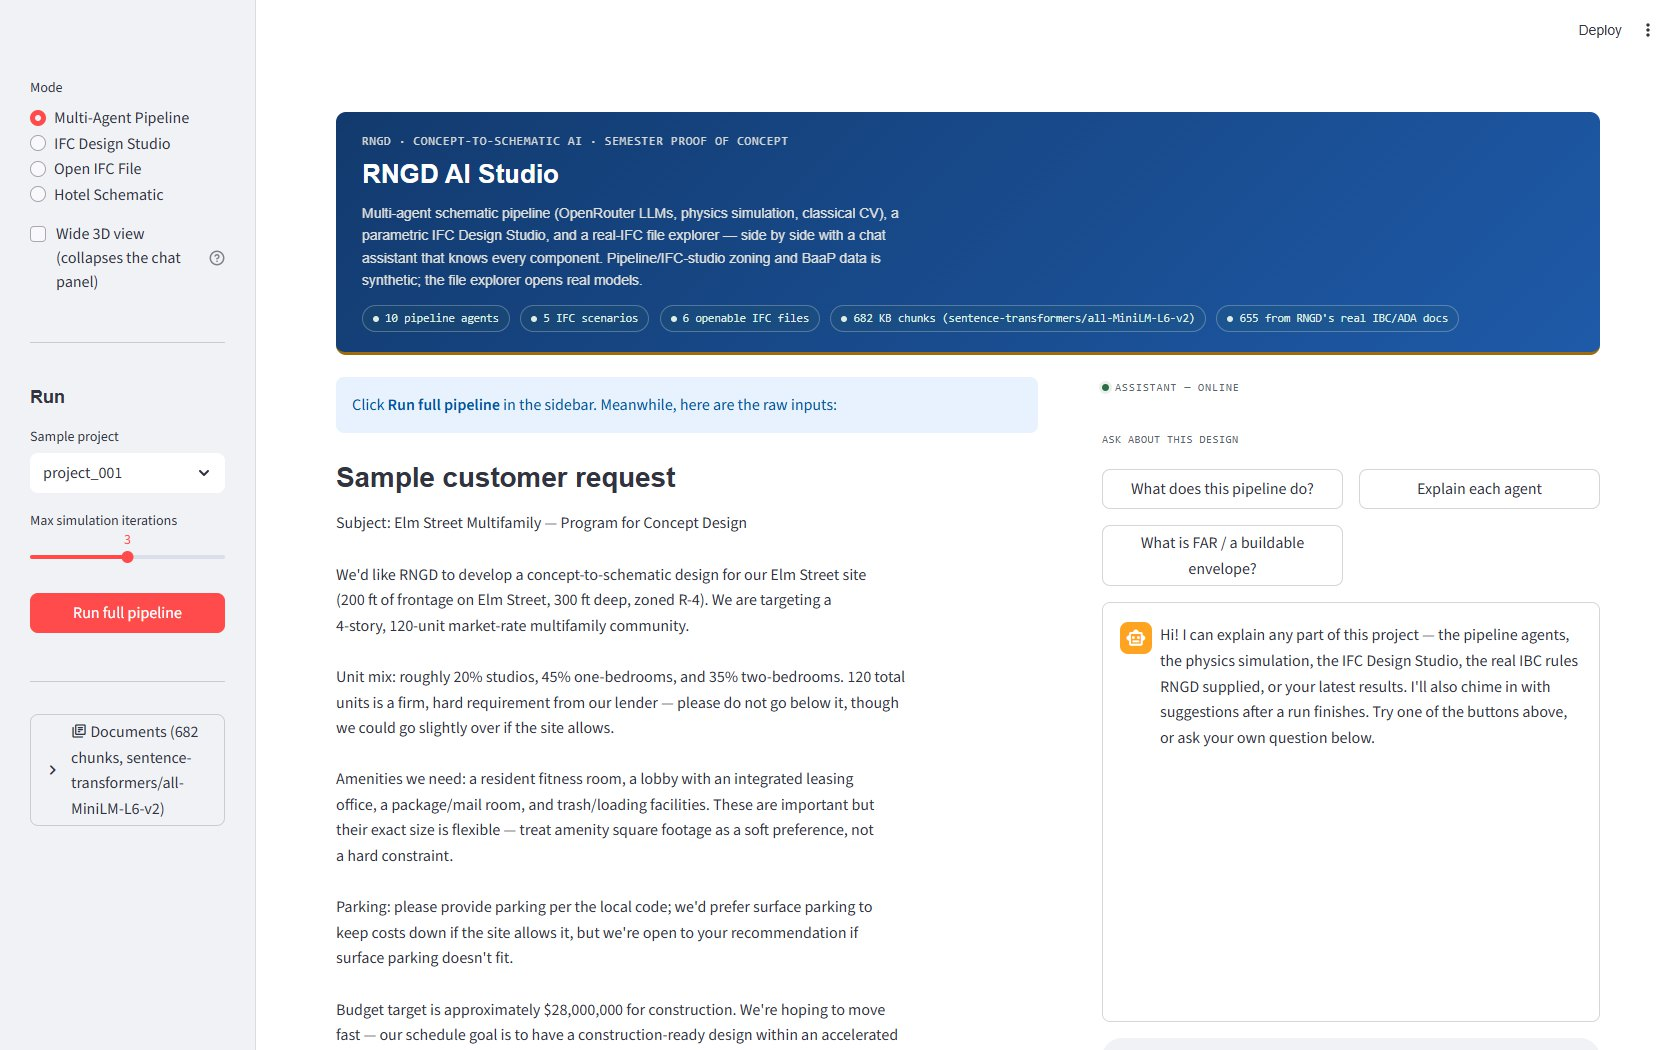
\includegraphics[width=0.92\linewidth,height=0.4\textheight,keepaspectratio]{figures/snap_01_pipeline_inputs}\caption*{\textbf{Screen 01.} Multi-Agent Pipeline before a run: the sample customer request and site sketch that feed the agents; the assistant panel on the right.}\end{figure}
\begin{figure}[H]\centering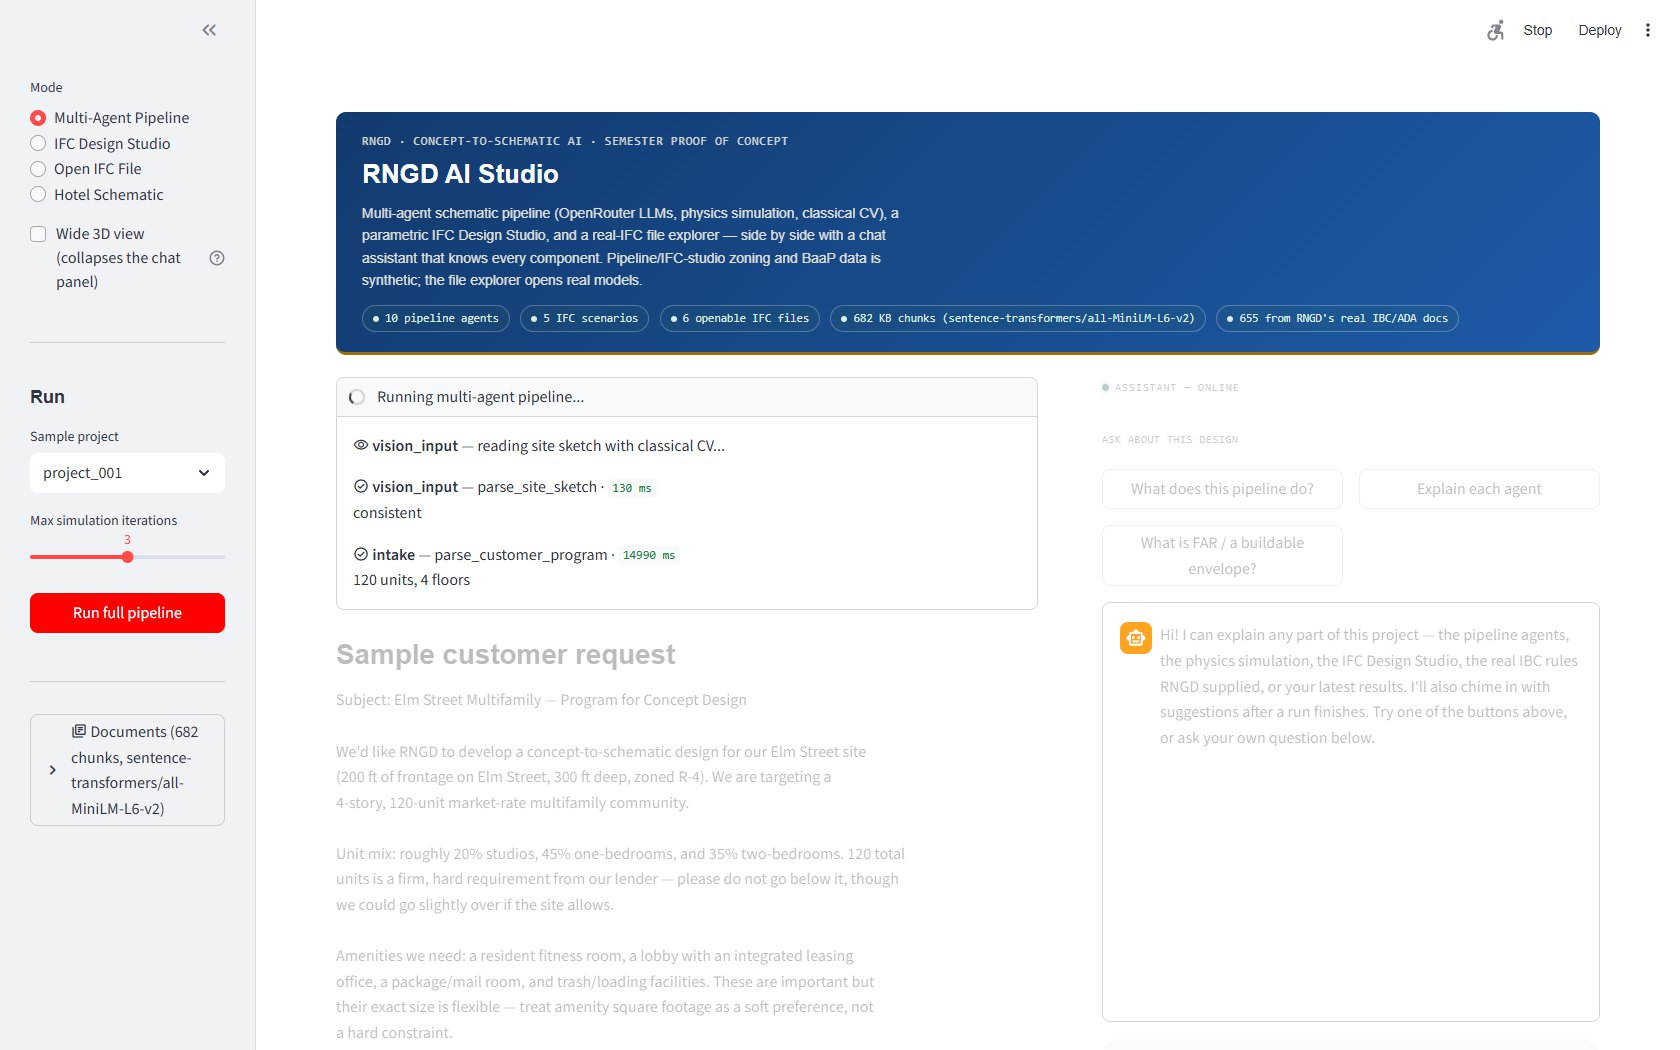
\includegraphics[width=0.92\linewidth,height=0.4\textheight,keepaspectratio]{figures/snap_02_pipeline_running}\caption*{\textbf{Screen 02.} The pipeline running live: each agent reports its step as it finishes.}\end{figure}
\begin{figure}[H]\centering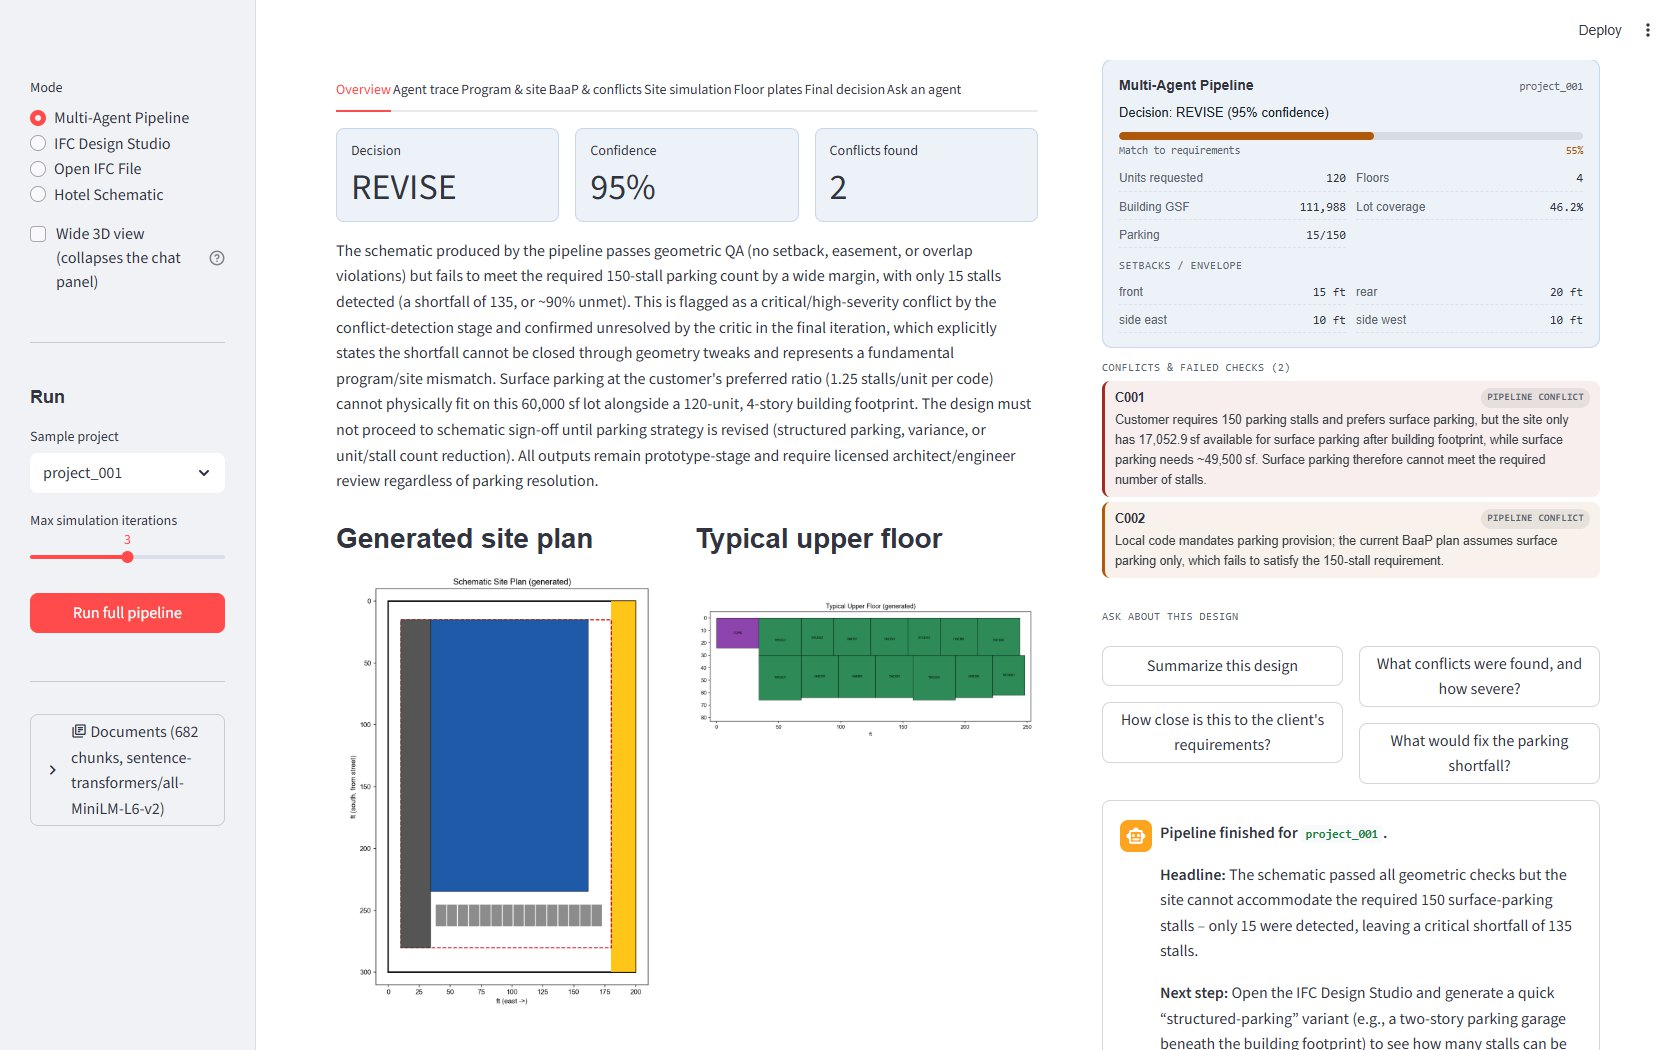
\includegraphics[width=0.92\linewidth,height=0.4\textheight,keepaspectratio]{figures/snap_03_pipeline_overview}\caption*{\textbf{Screen 03.} Pipeline result overview: the arbiter's decision, confidence and conflict count.}\end{figure}
\begin{figure}[H]\centering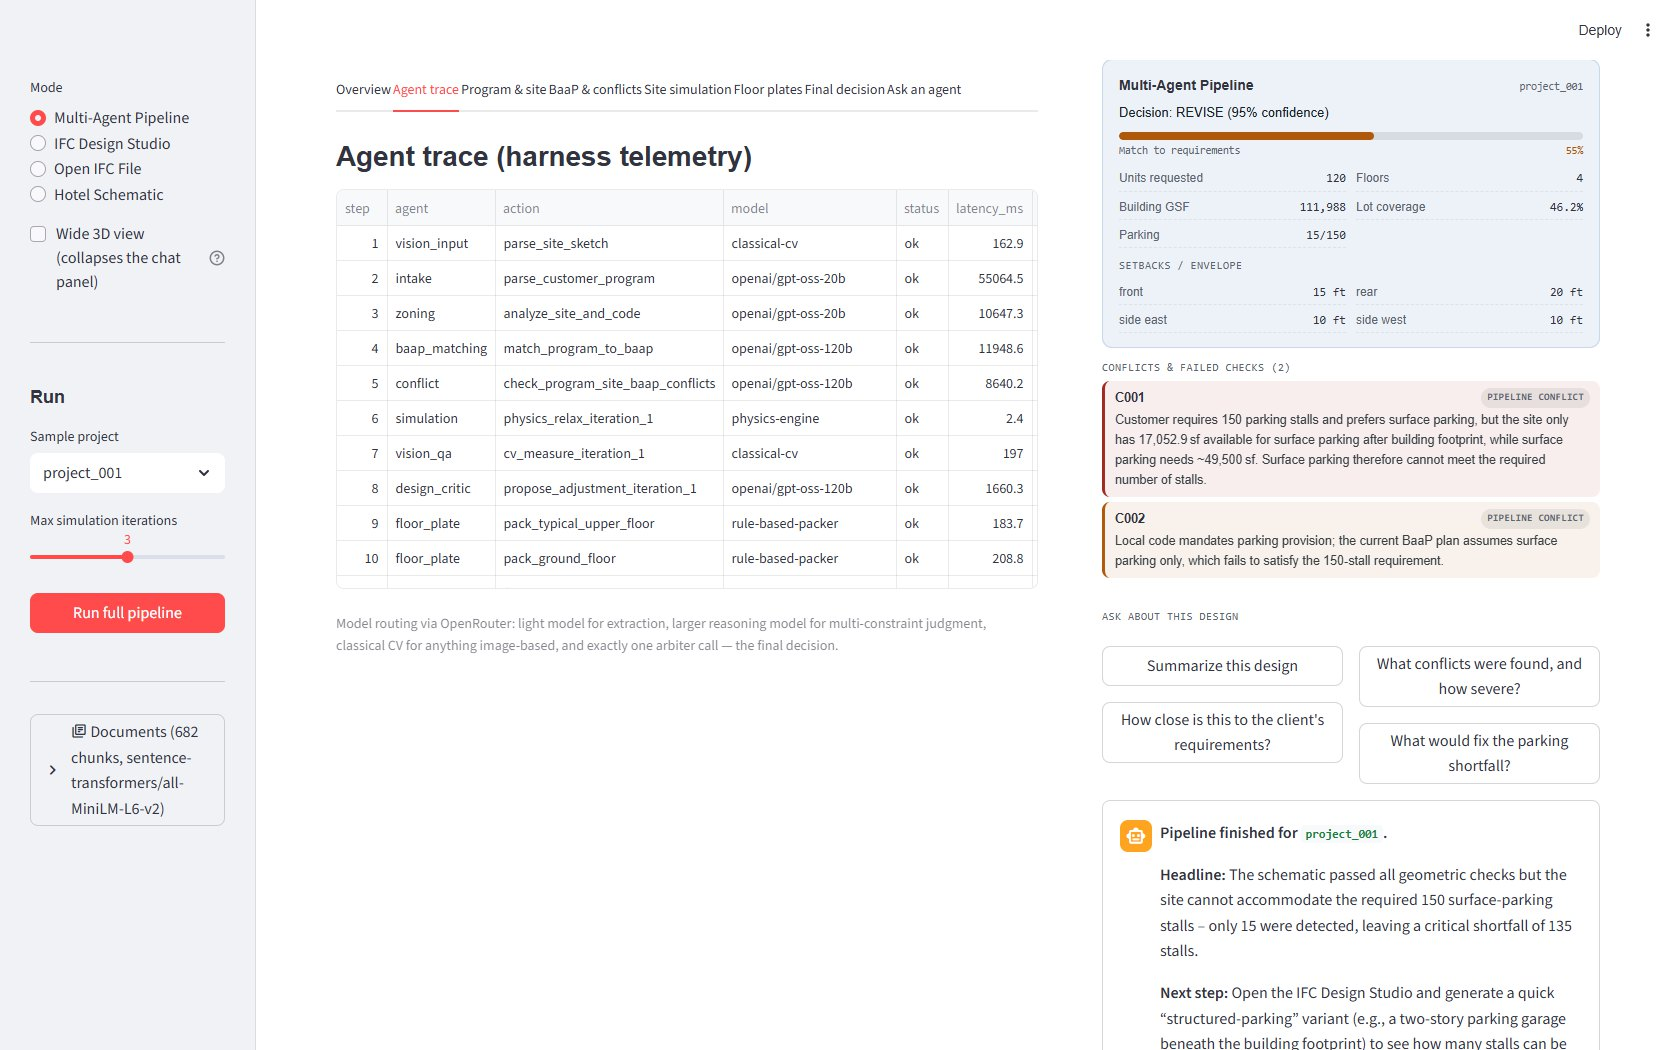
\includegraphics[width=0.92\linewidth,height=0.4\textheight,keepaspectratio]{figures/snap_04_pipeline_agent_trace}\caption*{\textbf{Screen 04.} Agent trace: every agent step with model, status and latency.}\end{figure}
\begin{figure}[H]\centering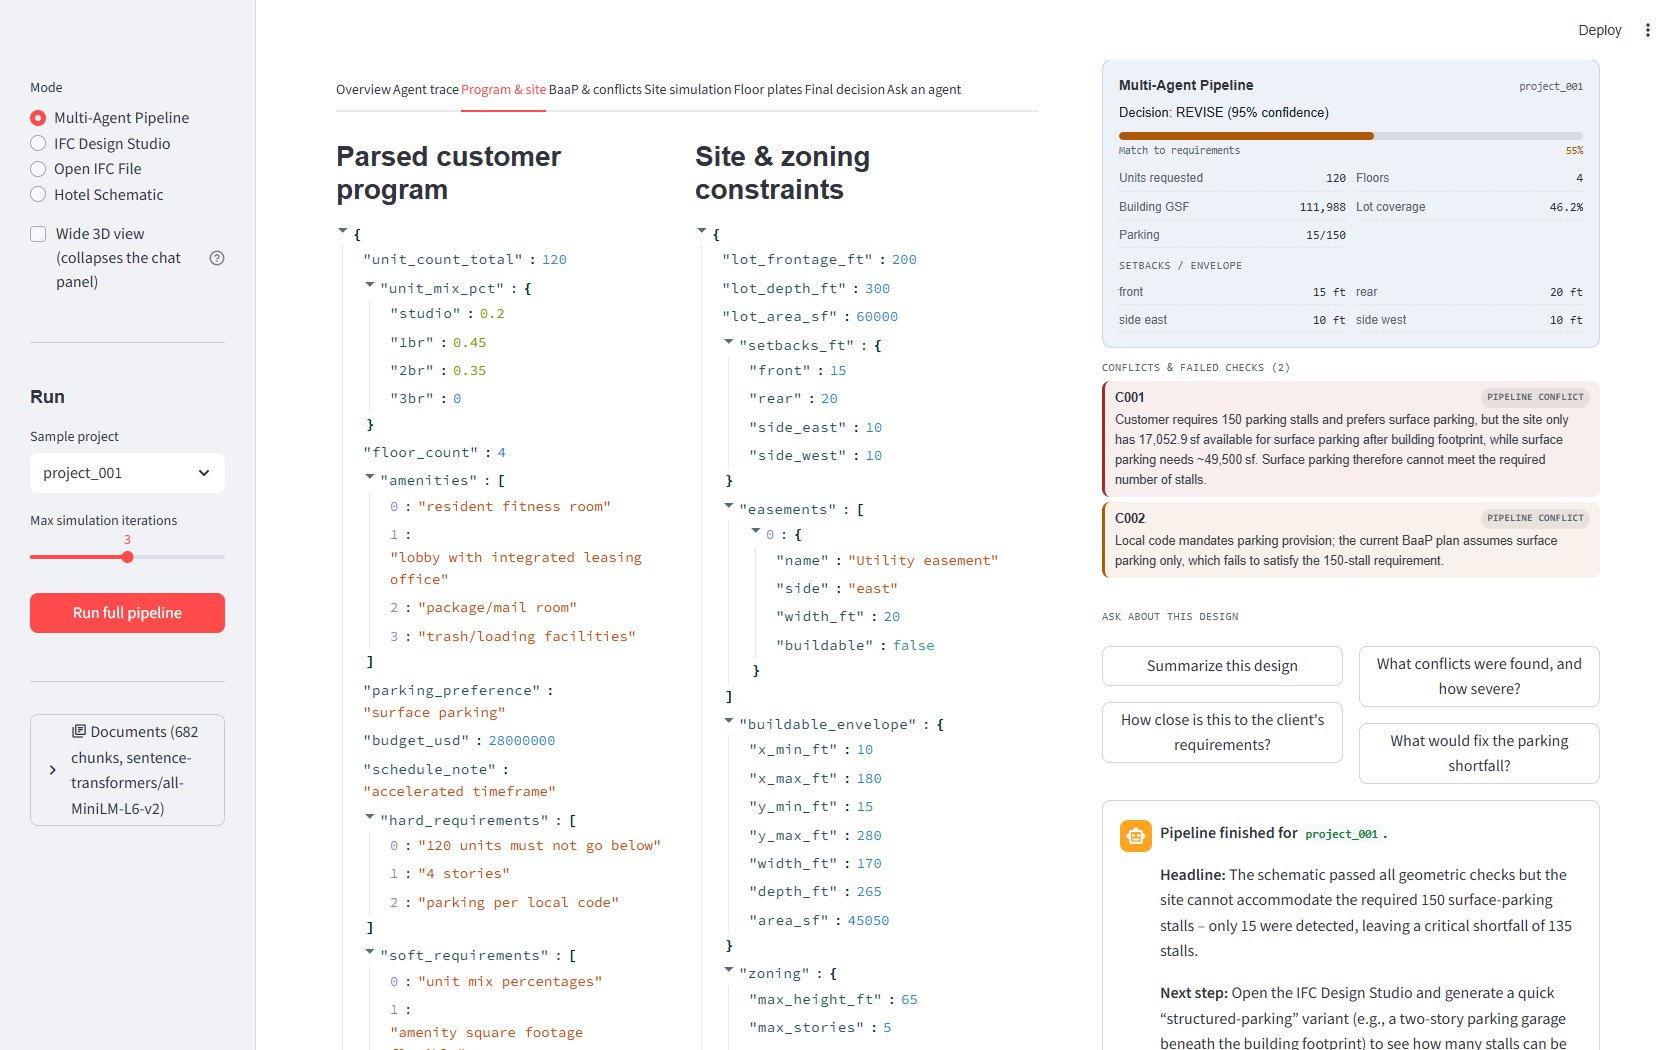
\includegraphics[width=0.92\linewidth,height=0.4\textheight,keepaspectratio]{figures/snap_05_pipeline_program_site}\caption*{\textbf{Screen 05.} Program parsed from the request and the computed site constraints.}\end{figure}
\begin{figure}[H]\centering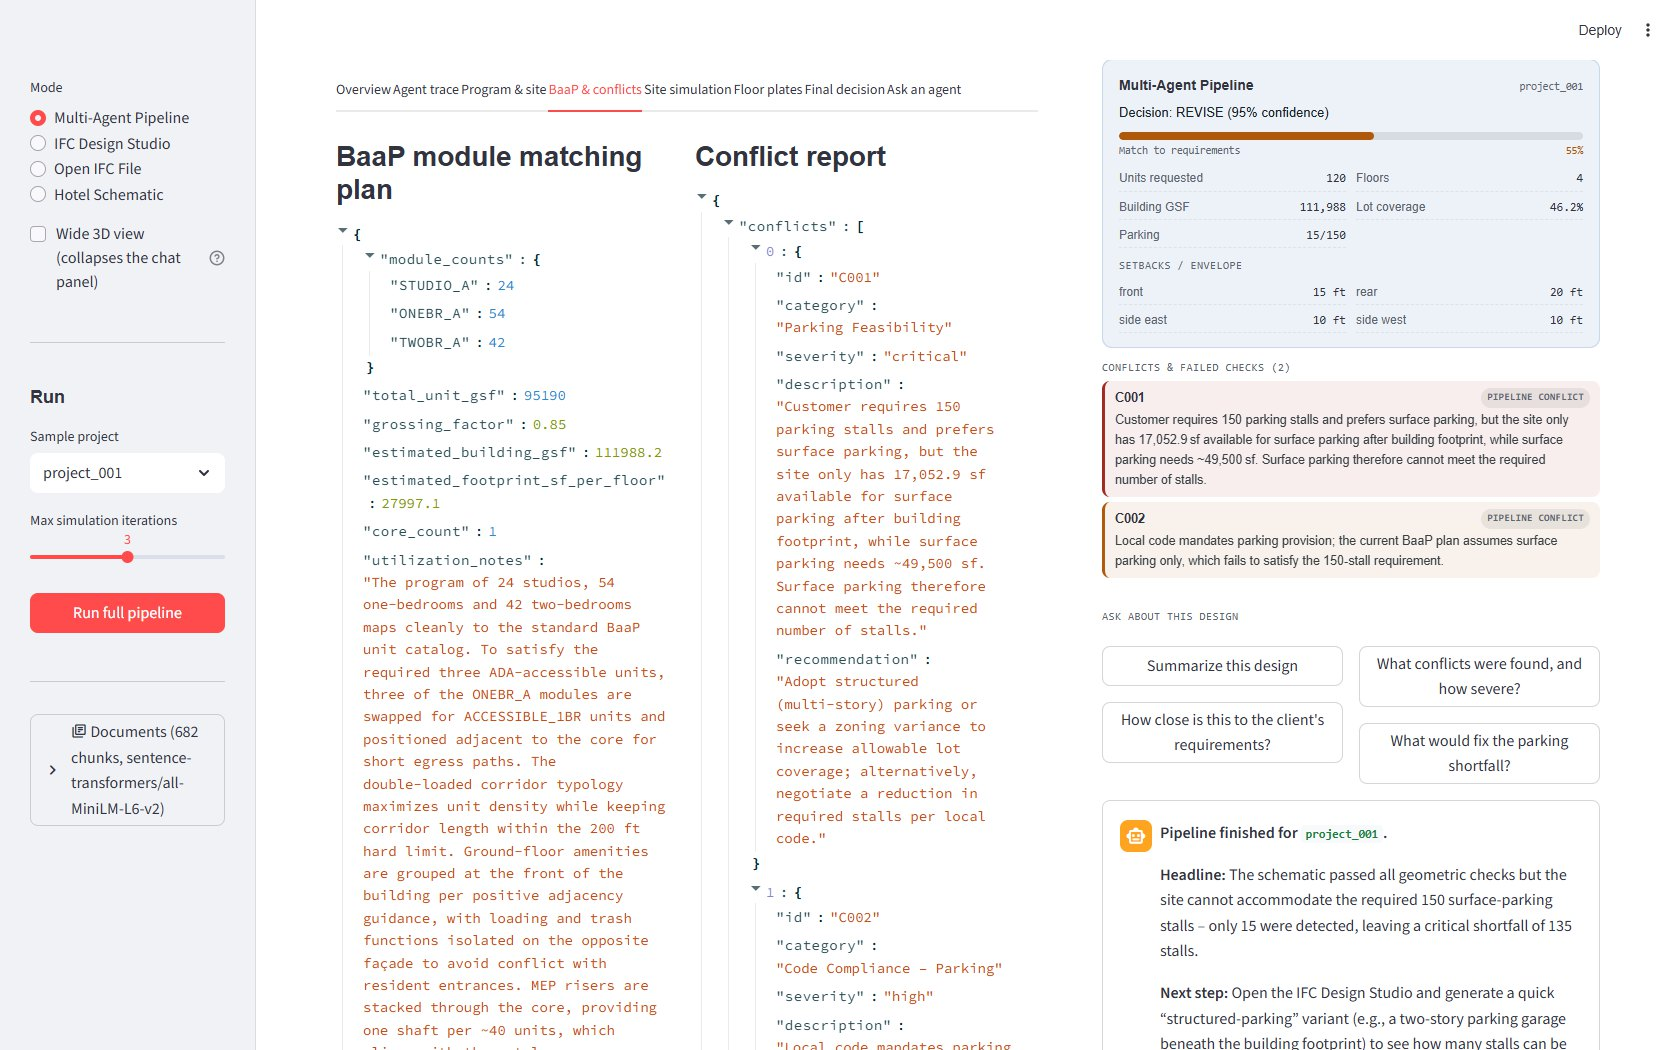
\includegraphics[width=0.92\linewidth,height=0.4\textheight,keepaspectratio]{figures/snap_06_pipeline_baap_conflicts}\caption*{\textbf{Screen 06.} BaaP module counts and the conflicts the Conflict Agent found.}\end{figure}
\begin{figure}[H]\centering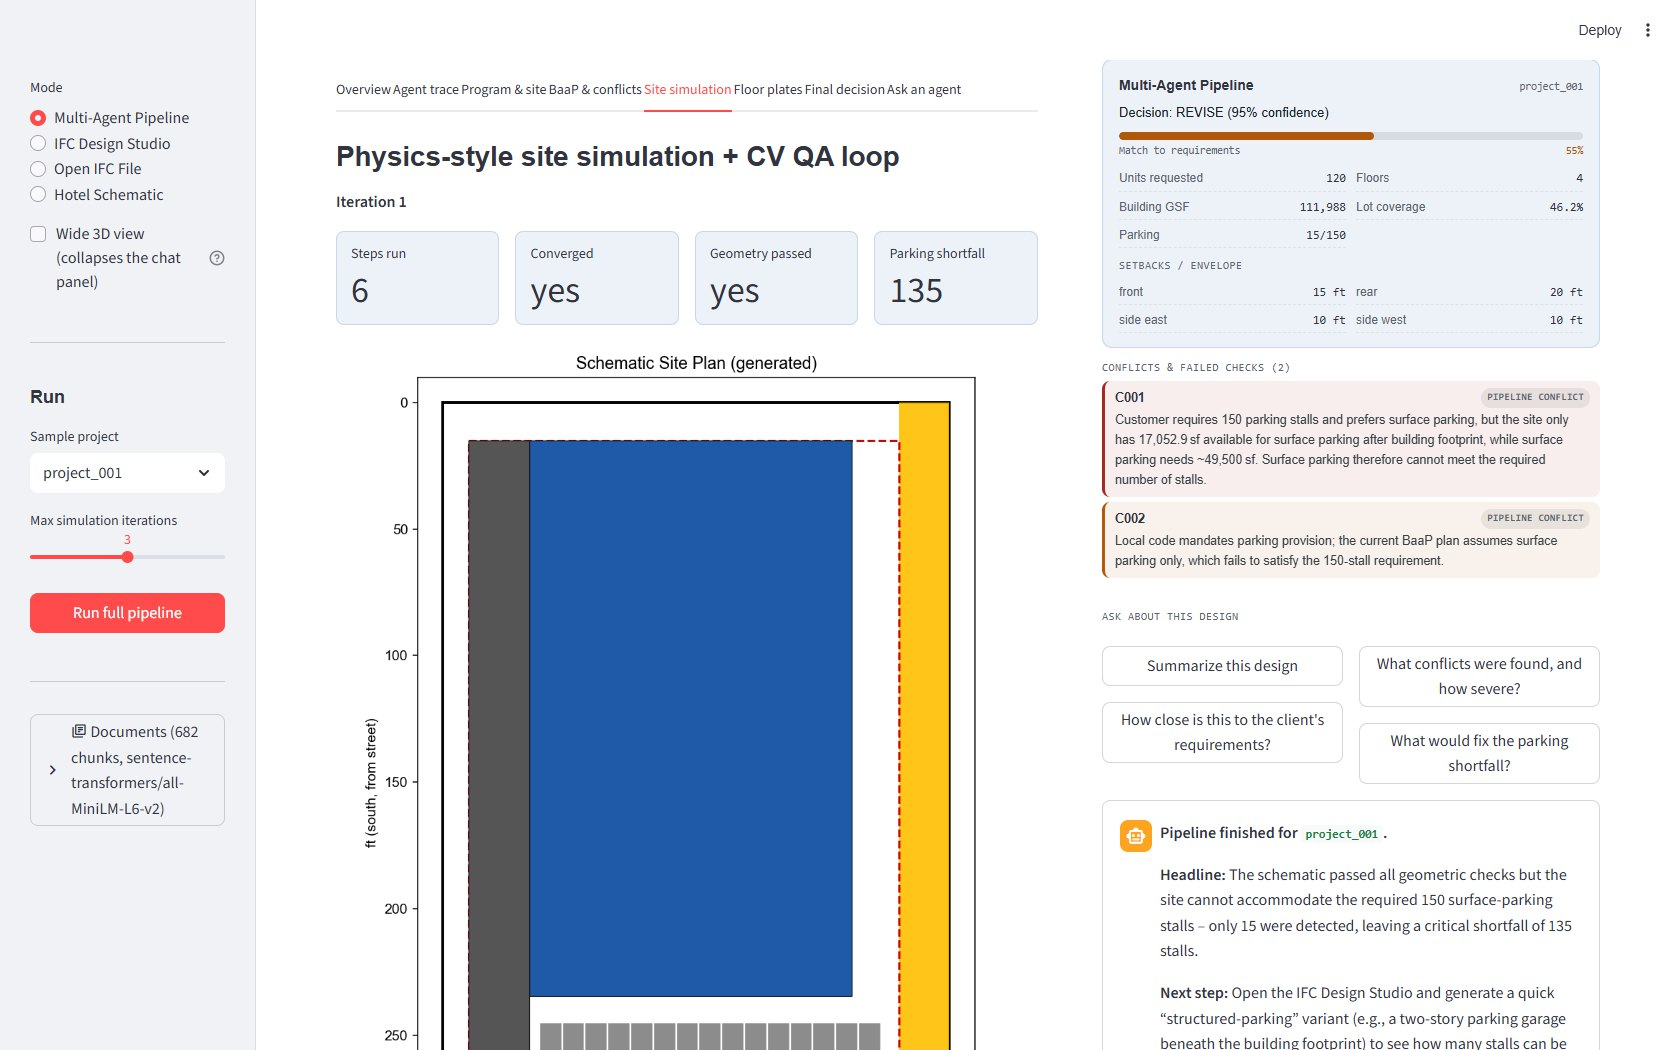
\includegraphics[width=0.92\linewidth,height=0.4\textheight,keepaspectratio]{figures/snap_07_pipeline_site_simulation}\caption*{\textbf{Screen 07.} Physics-style site simulation and the computer-vision QA of the rendered plan.}\end{figure}
\begin{figure}[H]\centering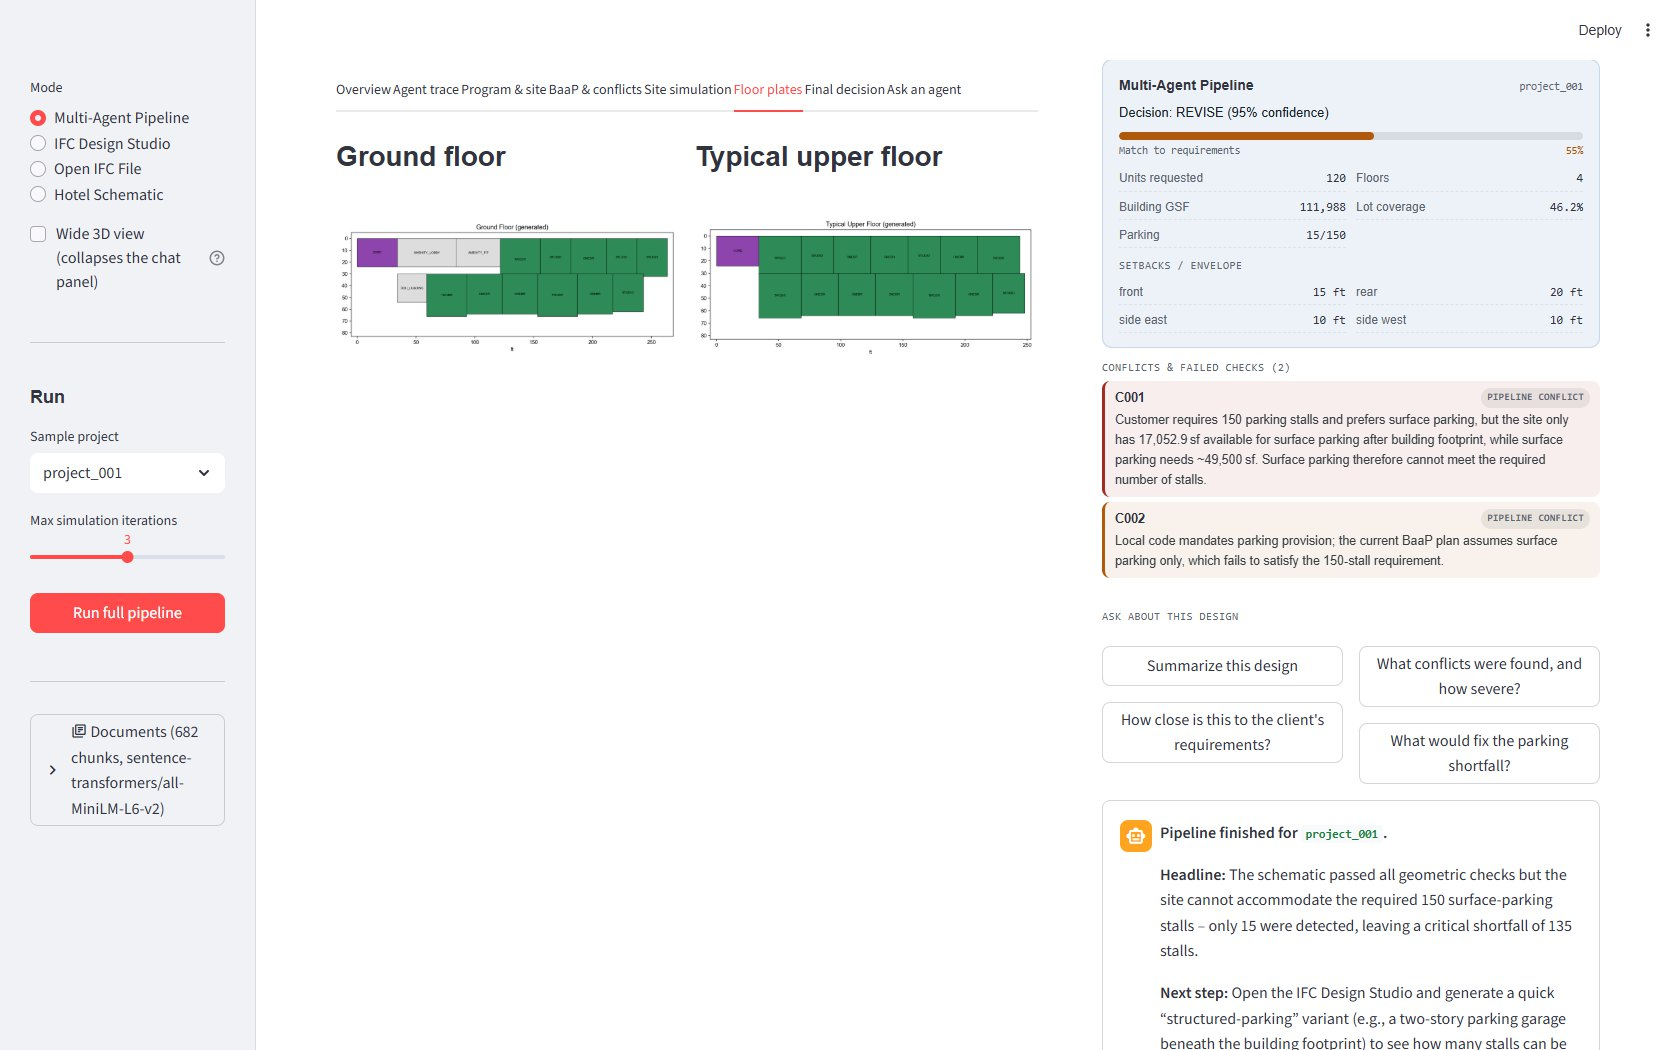
\includegraphics[width=0.92\linewidth,height=0.4\textheight,keepaspectratio]{figures/snap_08_pipeline_floor_plates}\caption*{\textbf{Screen 08.} Rule-based floor plates (ground and typical floor).}\end{figure}
\begin{figure}[H]\centering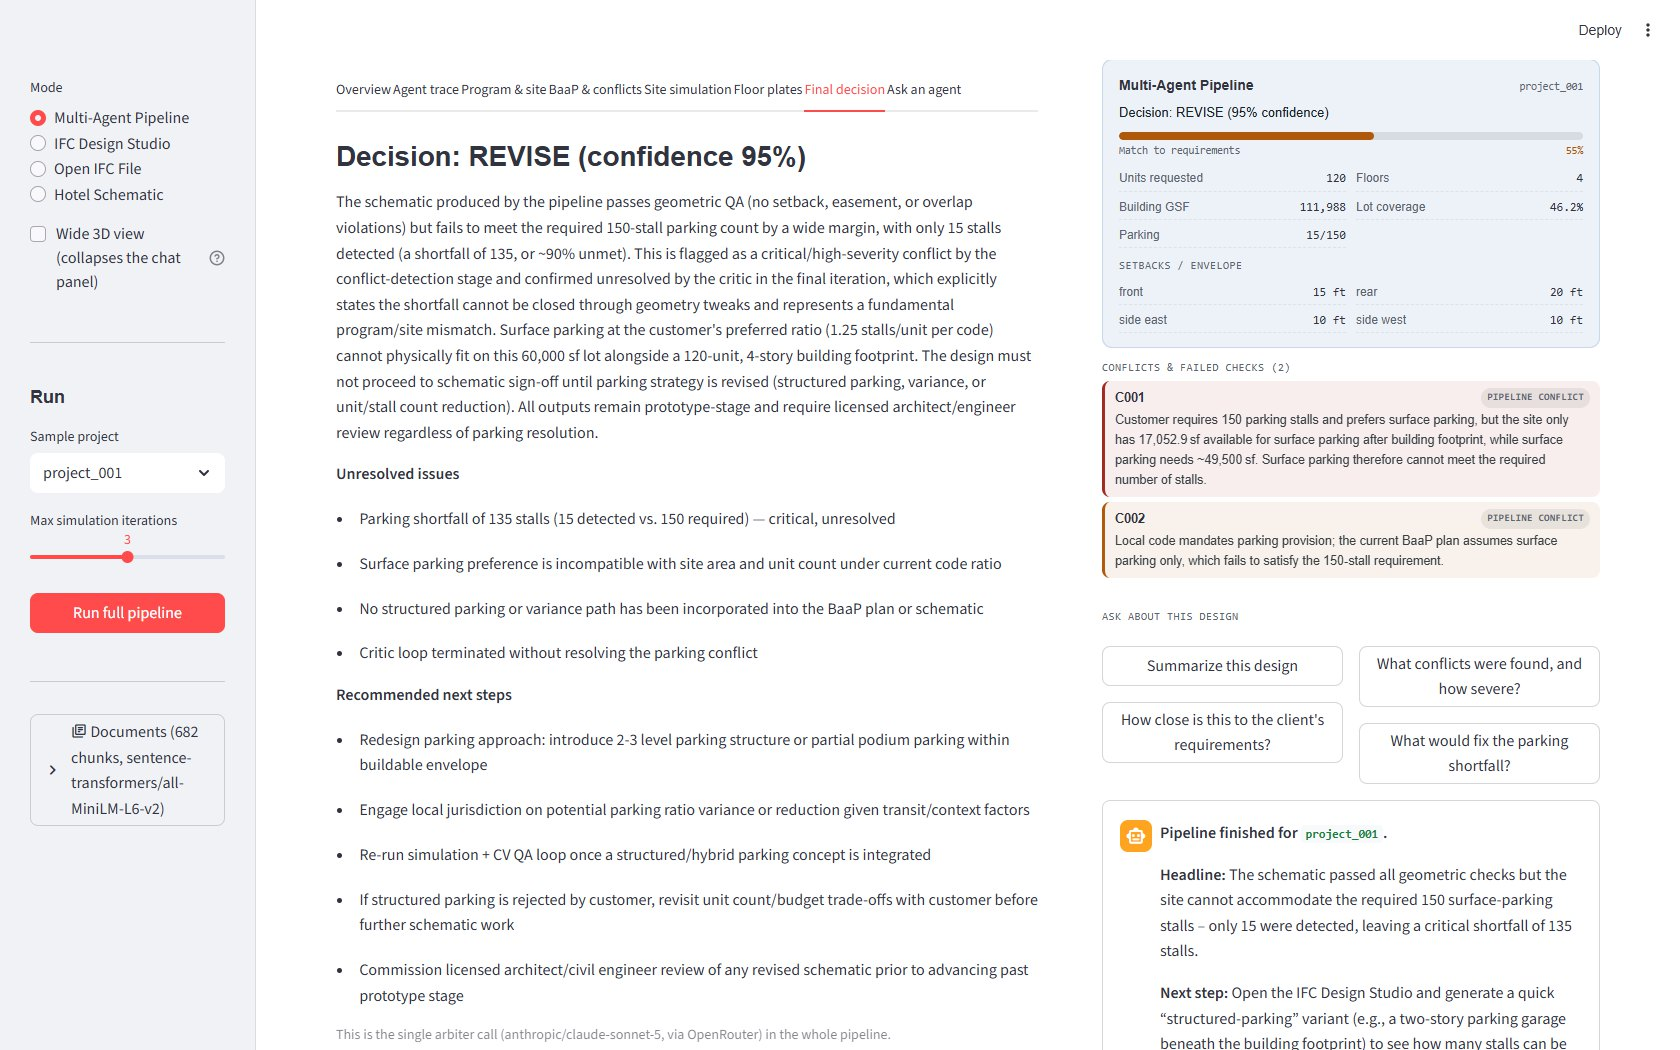
\includegraphics[width=0.92\linewidth,height=0.4\textheight,keepaspectratio]{figures/snap_09_pipeline_final_decision}\caption*{\textbf{Screen 09.} The arbiter's final decision, unresolved issues and next steps.}\end{figure}
\subsection*{IFC Design Studio}
\begin{figure}[H]\centering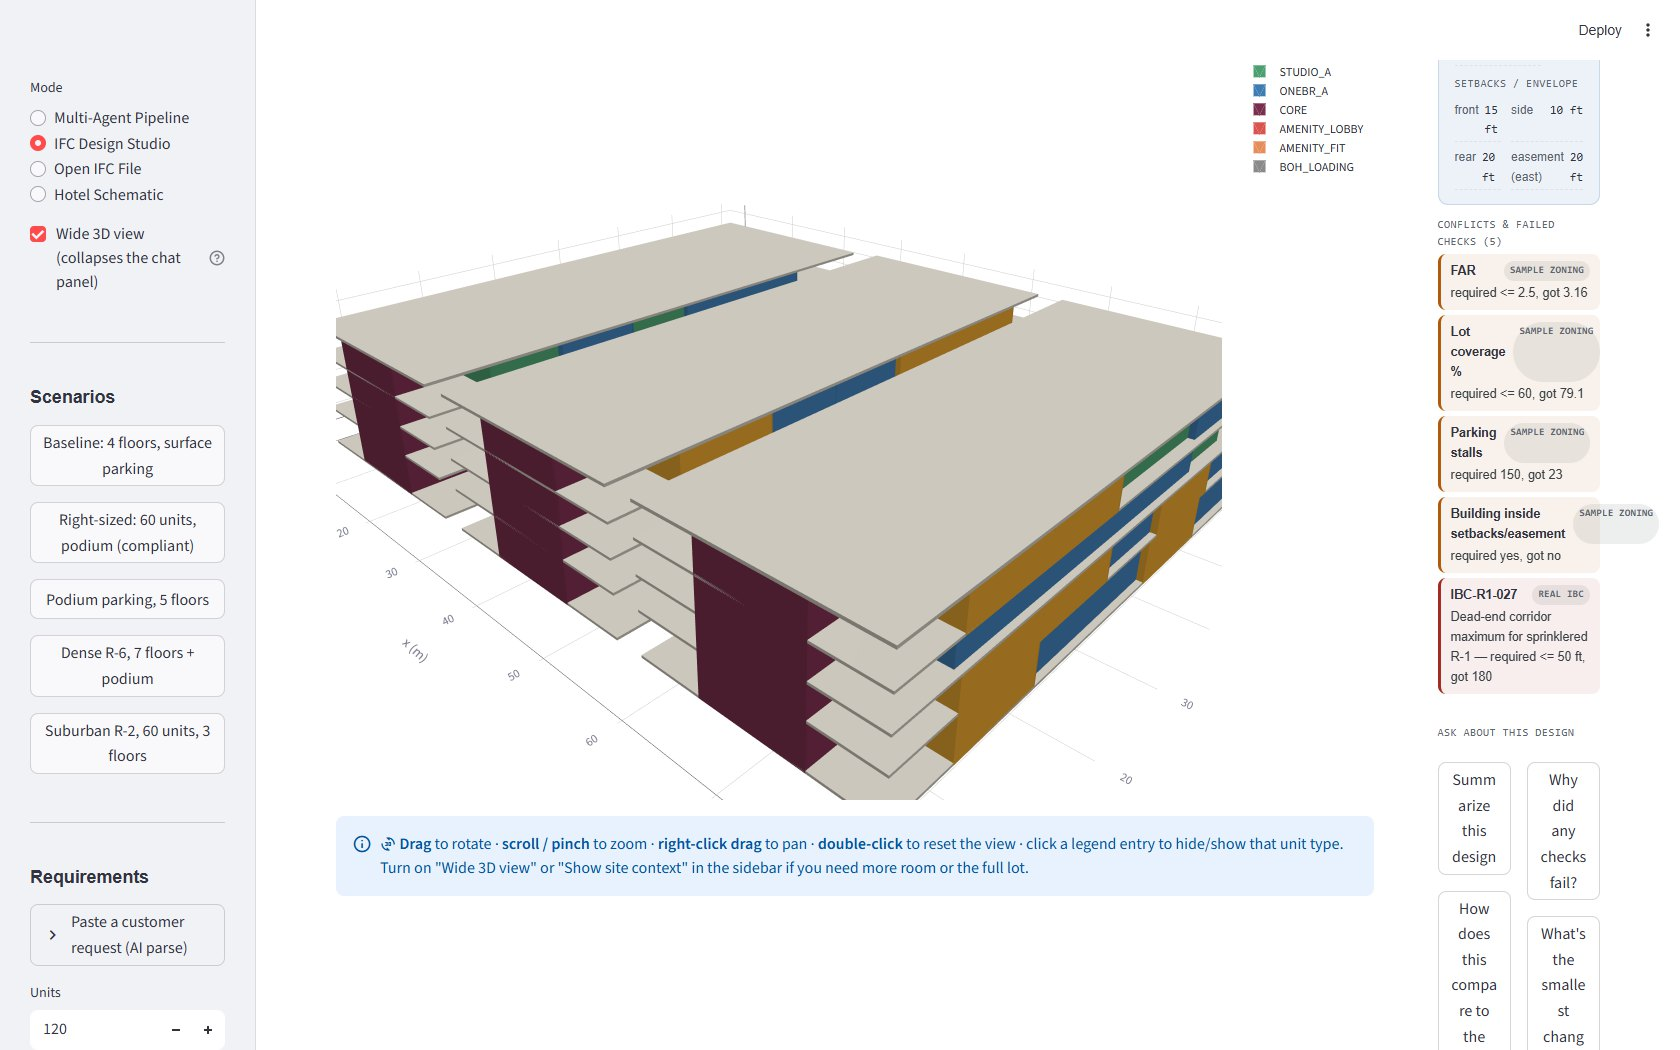
\includegraphics[width=0.92\linewidth,height=0.4\textheight,keepaspectratio]{figures/snap_10_ifc_baseline_3d_model}\caption*{\textbf{Screen 10.} IFC Design Studio, Baseline scenario (120 units, 4 floors, surface parking): the generated IFC4 model in the 3D viewer.}\end{figure}
\begin{figure}[H]\centering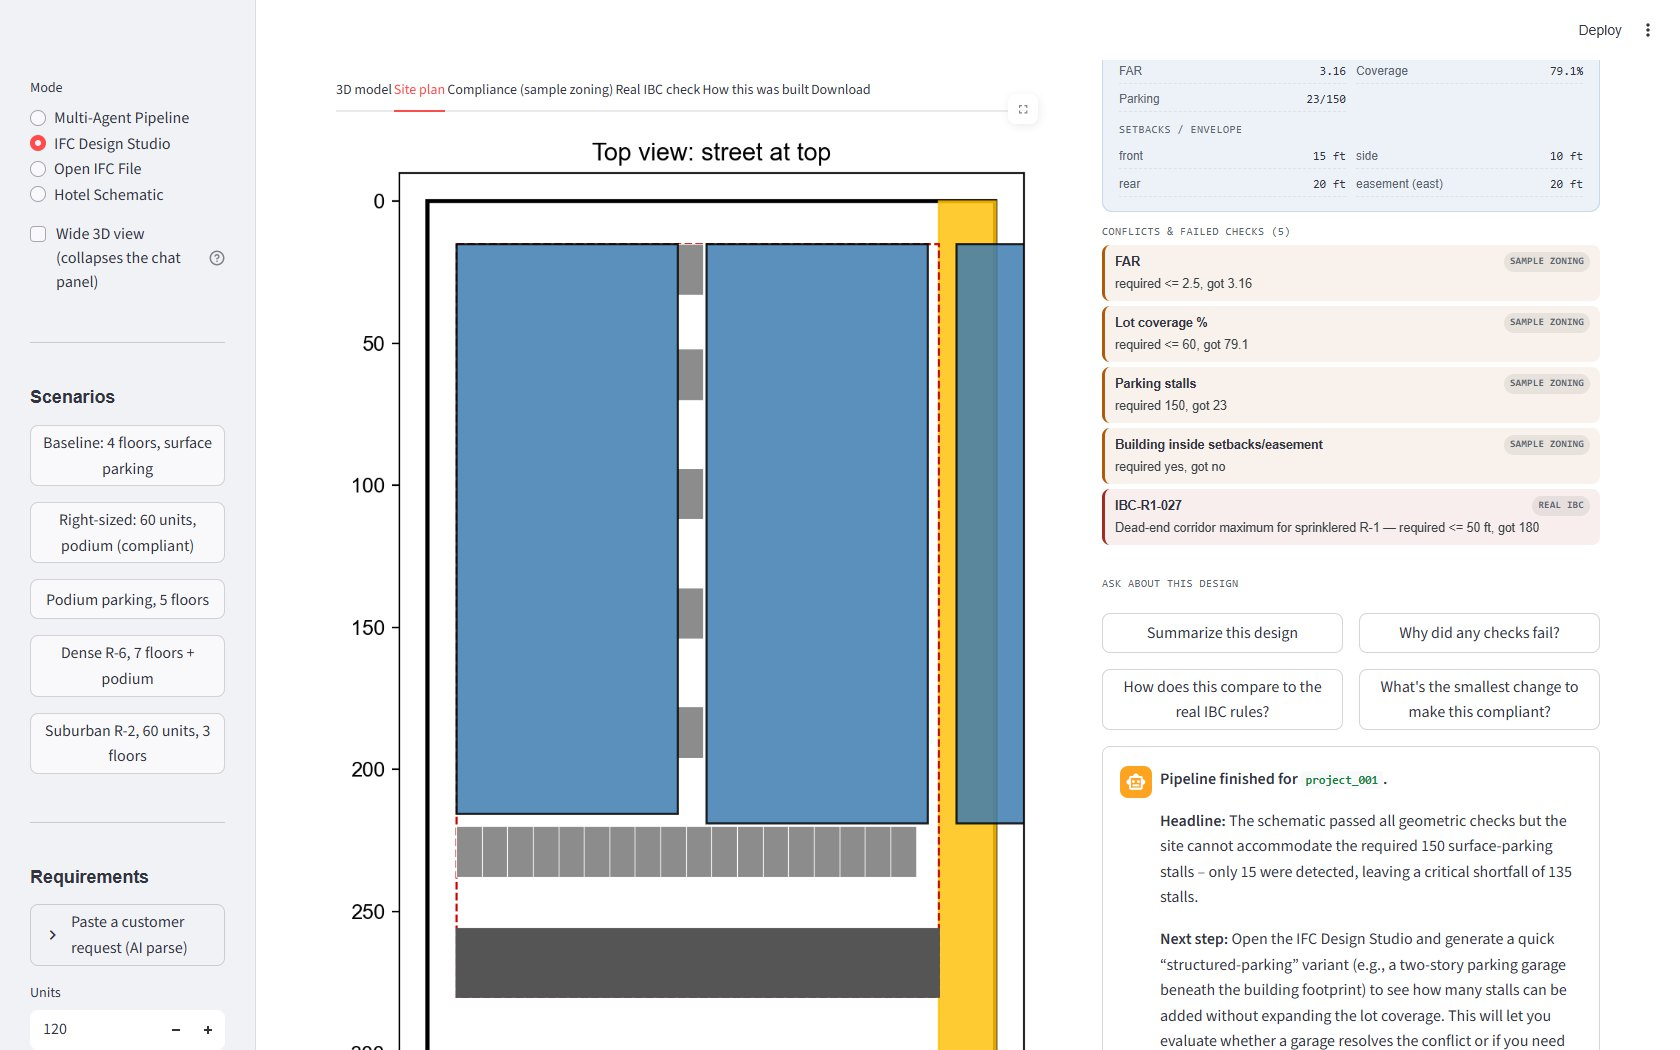
\includegraphics[width=0.92\linewidth,height=0.4\textheight,keepaspectratio]{figures/snap_11_ifc_baseline_site_plan}\caption*{\textbf{Screen 11.} Baseline site plan: building, parking, easement and fire lane on the synthetic lot.}\end{figure}
\begin{figure}[H]\centering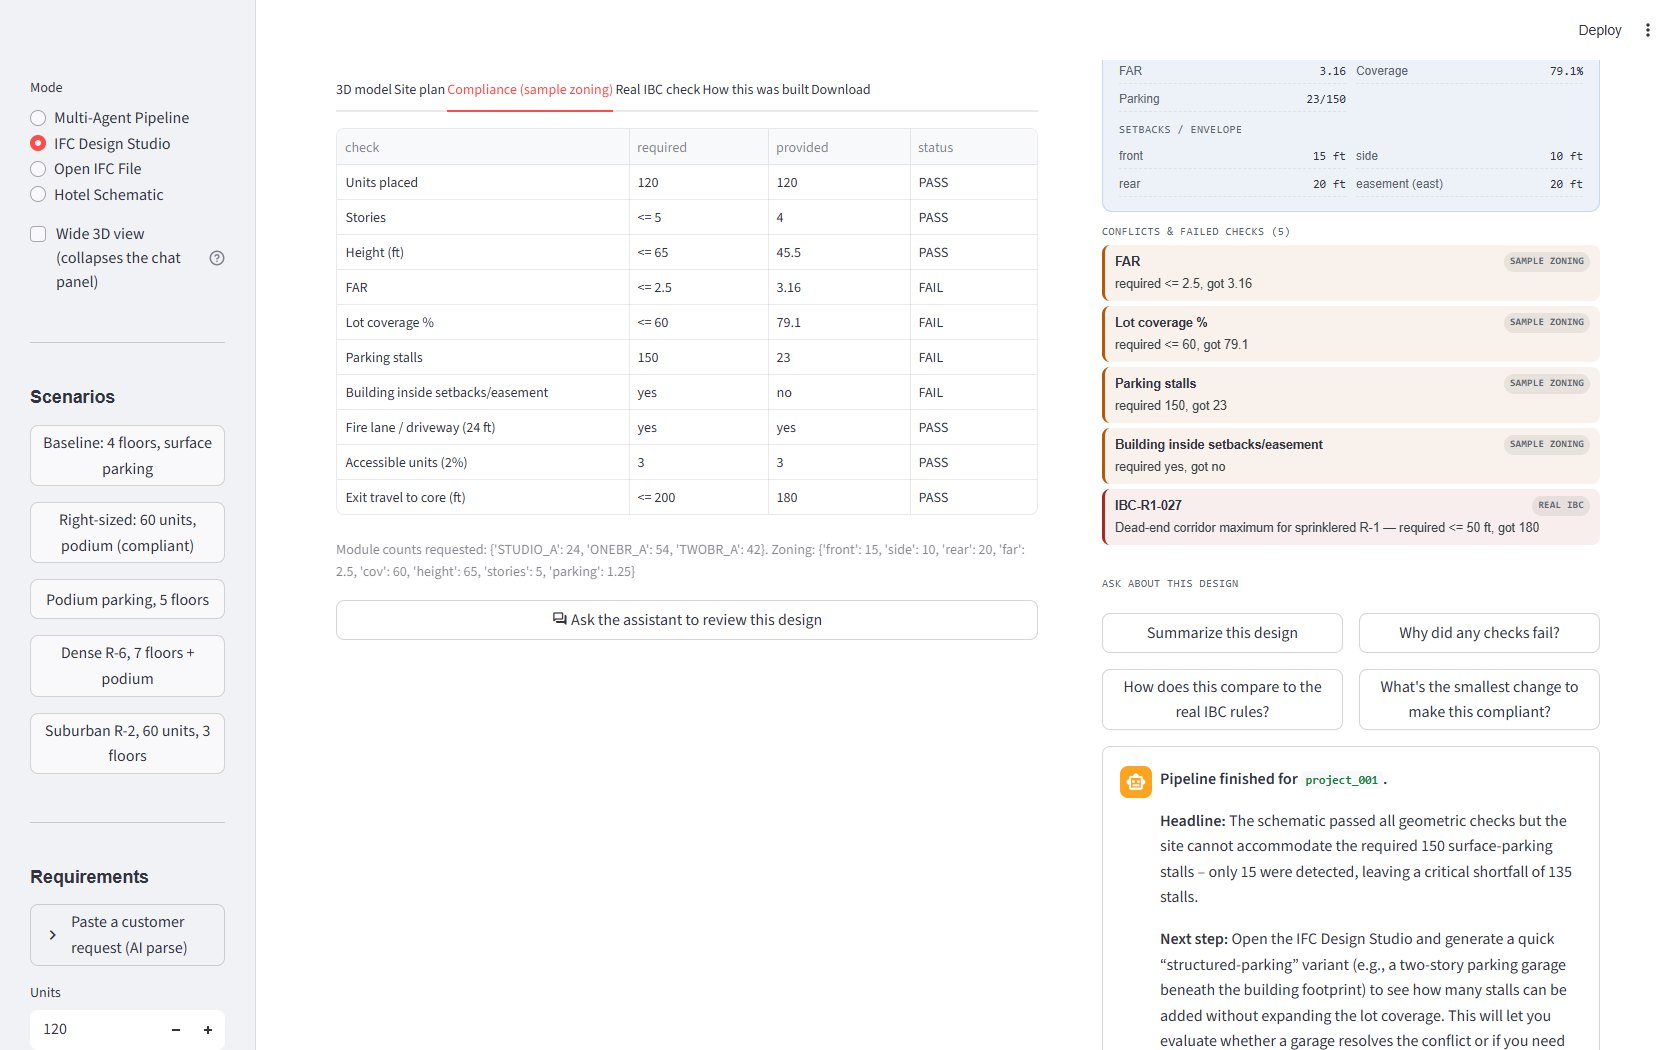
\includegraphics[width=0.92\linewidth,height=0.4\textheight,keepaspectratio]{figures/snap_12_ifc_baseline_compliance}\caption*{\textbf{Screen 12.} Baseline compliance against the ten sample-zoning checks.}\end{figure}
\begin{figure}[H]\centering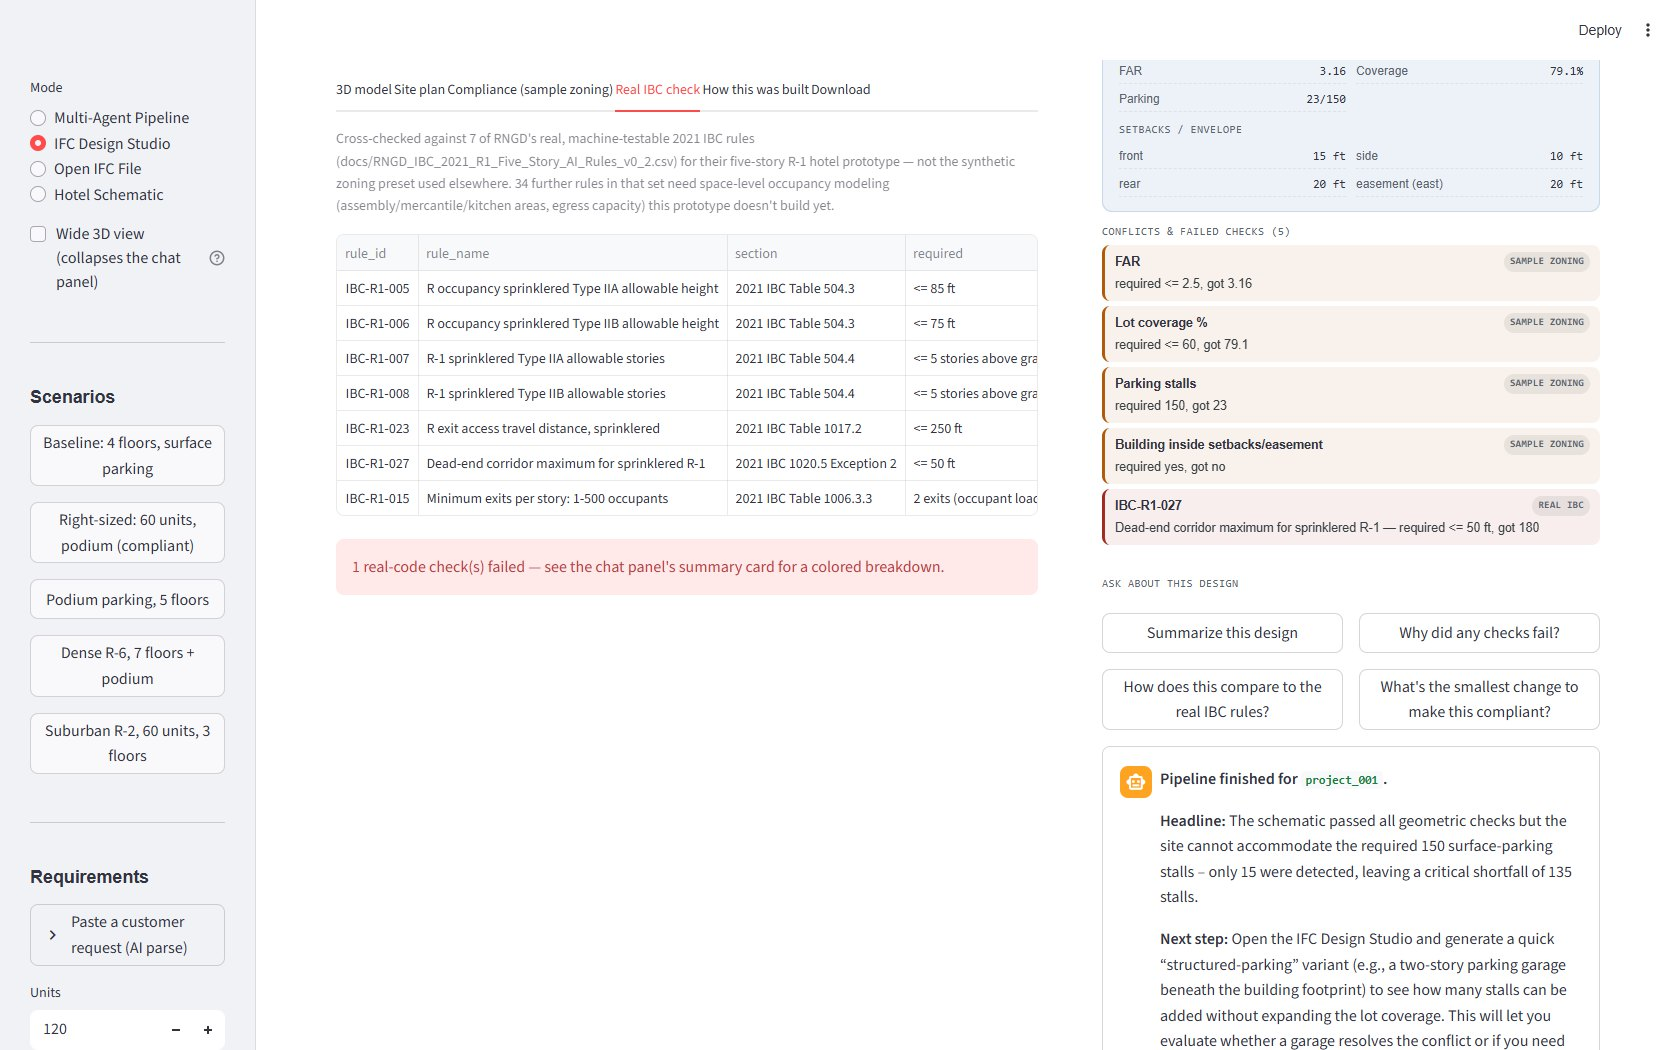
\includegraphics[width=0.92\linewidth,height=0.4\textheight,keepaspectratio]{figures/snap_13_ifc_baseline_real_ibc_check}\caption*{\textbf{Screen 13.} Baseline cross-checked against RNGD's real 2021 IBC rules.}\end{figure}
\begin{figure}[H]\centering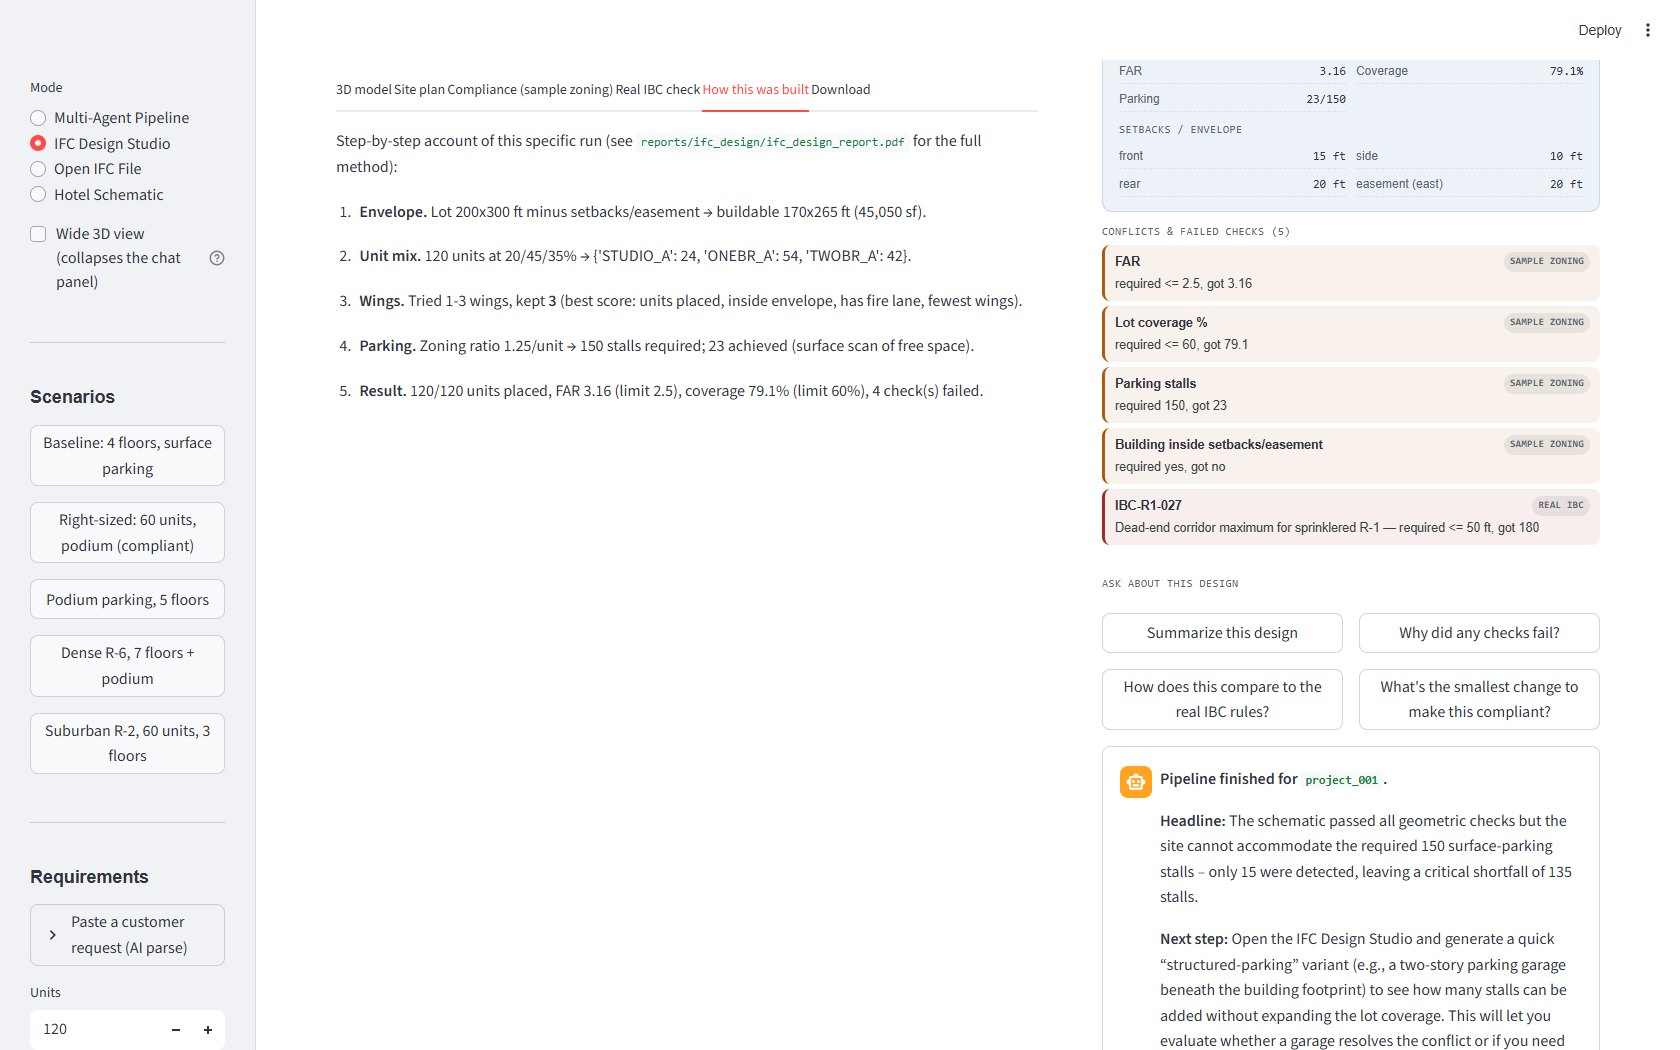
\includegraphics[width=0.92\linewidth,height=0.4\textheight,keepaspectratio]{figures/snap_14_ifc_baseline_how_this_was_built}\caption*{\textbf{Screen 14.} Step-by-step explanation of how the layout was generated.}\end{figure}
\begin{figure}[H]\centering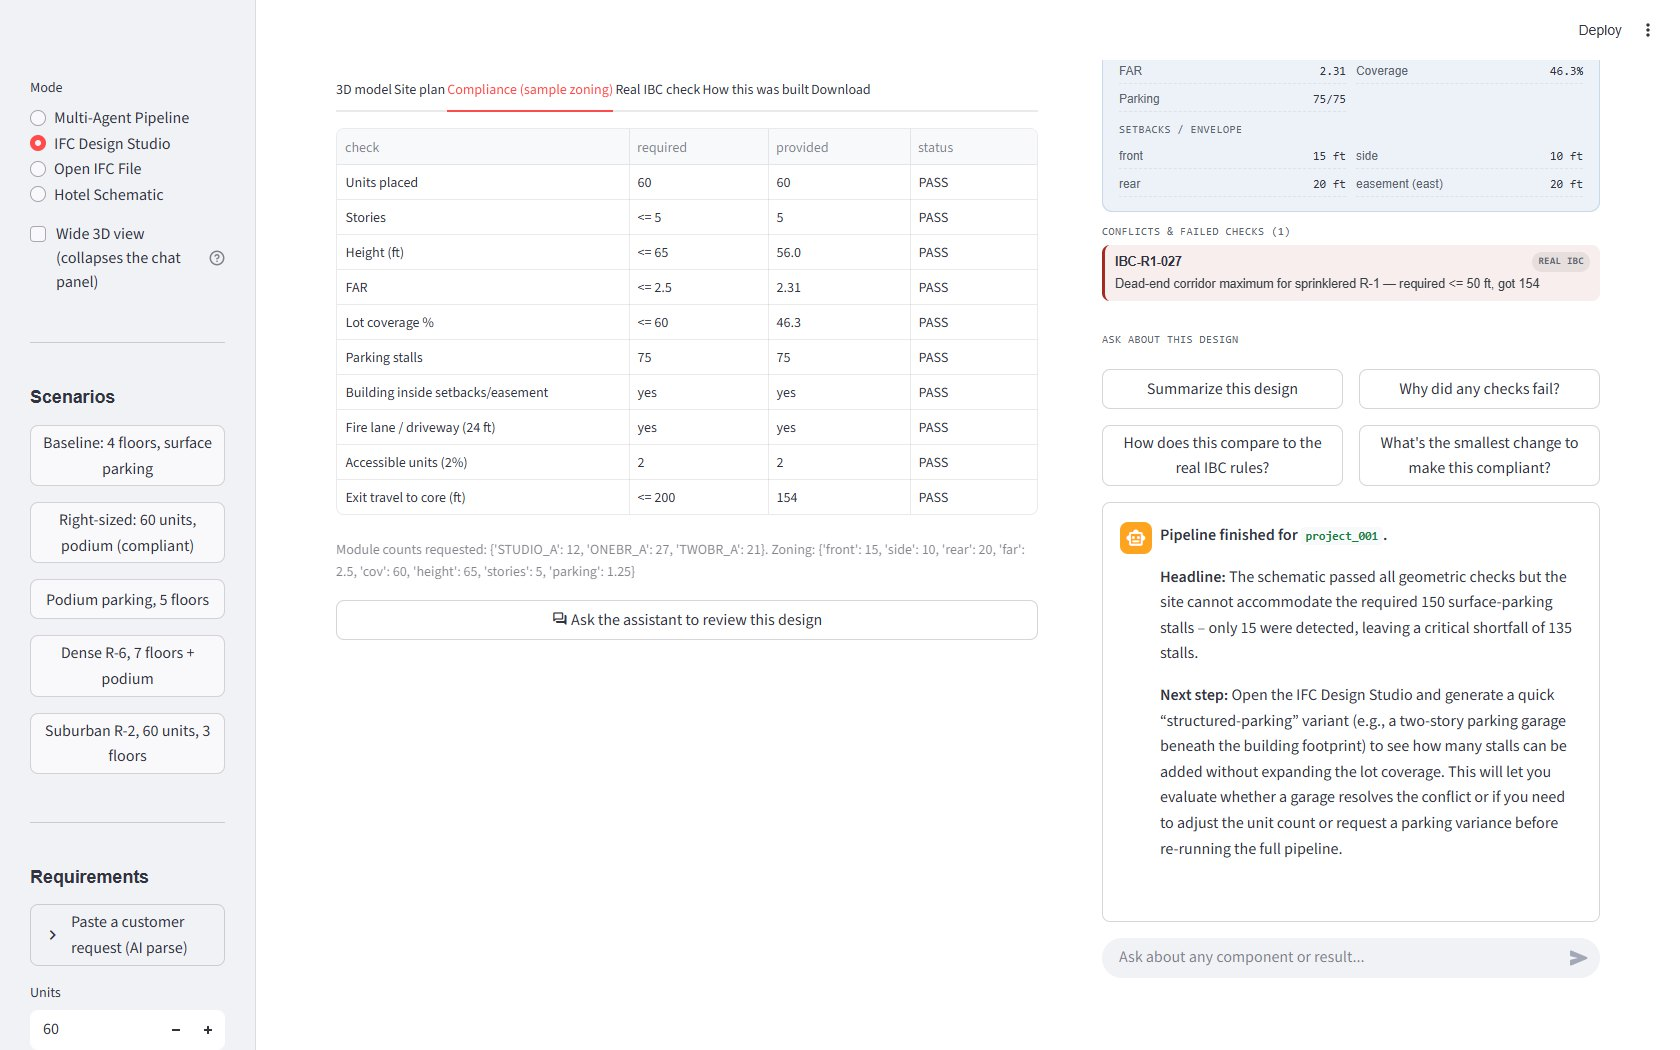
\includegraphics[width=0.92\linewidth,height=0.4\textheight,keepaspectratio]{figures/snap_15_ifc_rightsized_compliance}\caption*{\textbf{Screen 15.} Right-sized scenario (60 units, podium parking): the compliance checks after the fix.}\end{figure}
\begin{figure}[H]\centering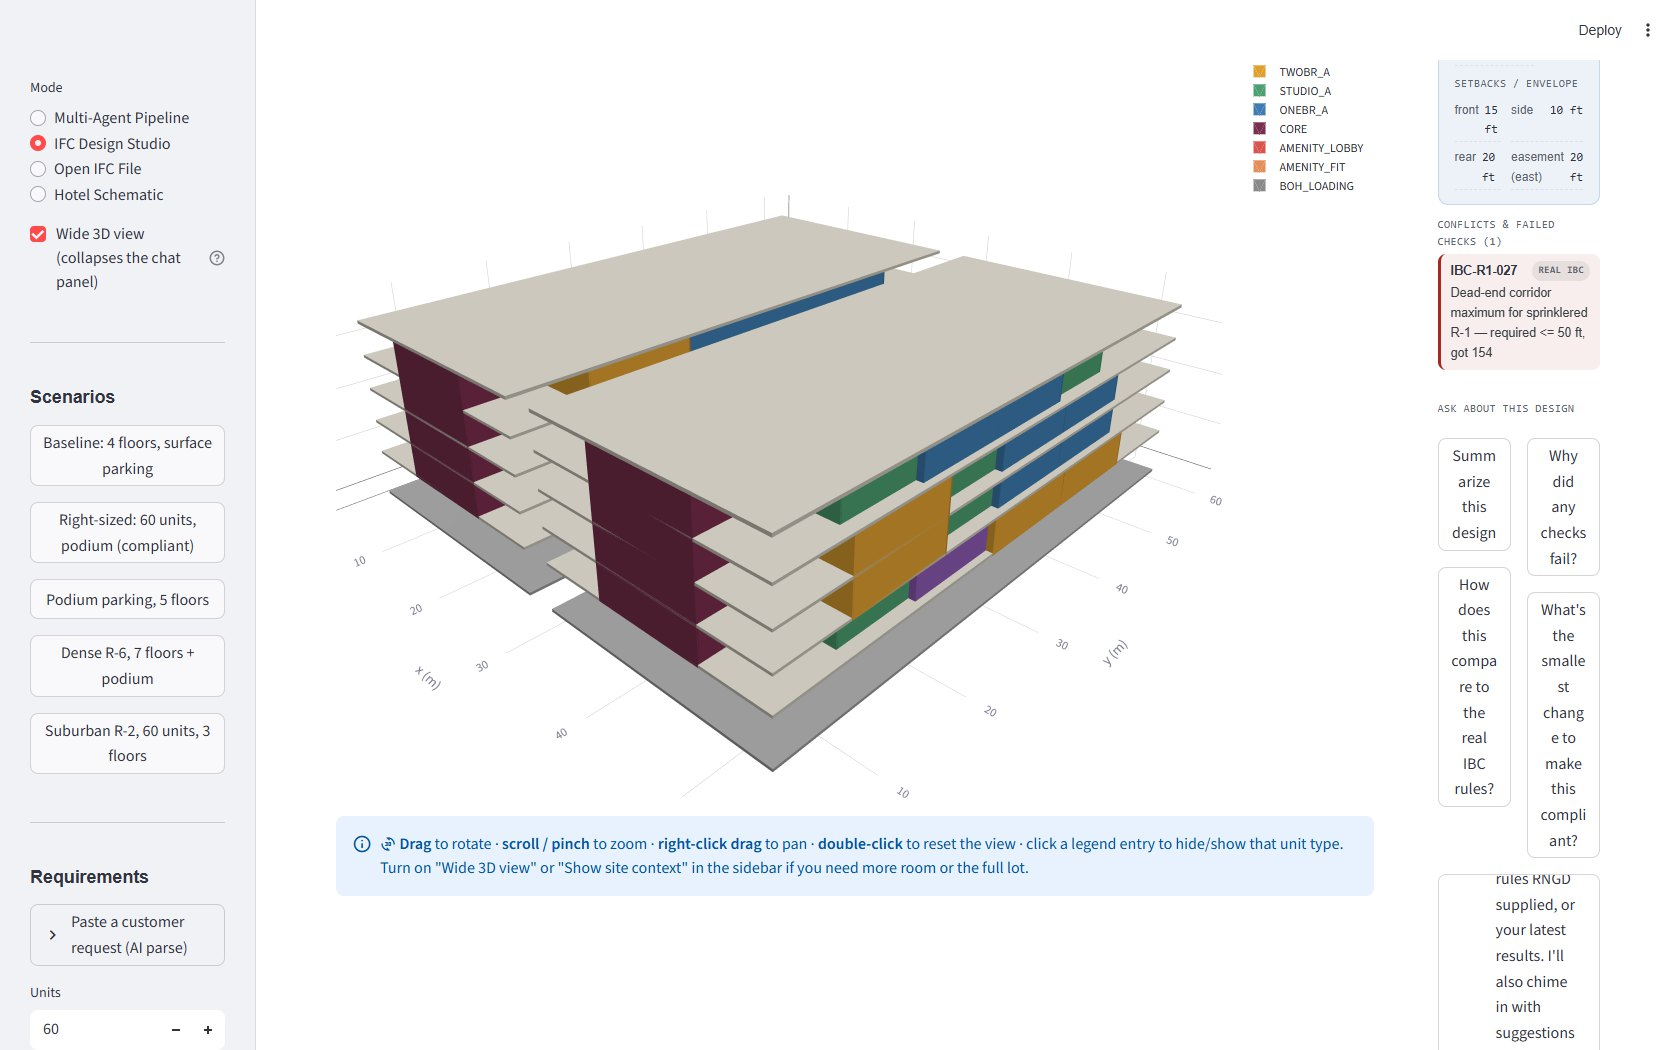
\includegraphics[width=0.92\linewidth,height=0.4\textheight,keepaspectratio]{figures/snap_16_ifc_rightsized_3d}\caption*{\textbf{Screen 16.} Right-sized scenario in 3D.}\end{figure}
\subsection*{Open IFC File}
\begin{figure}[H]\centering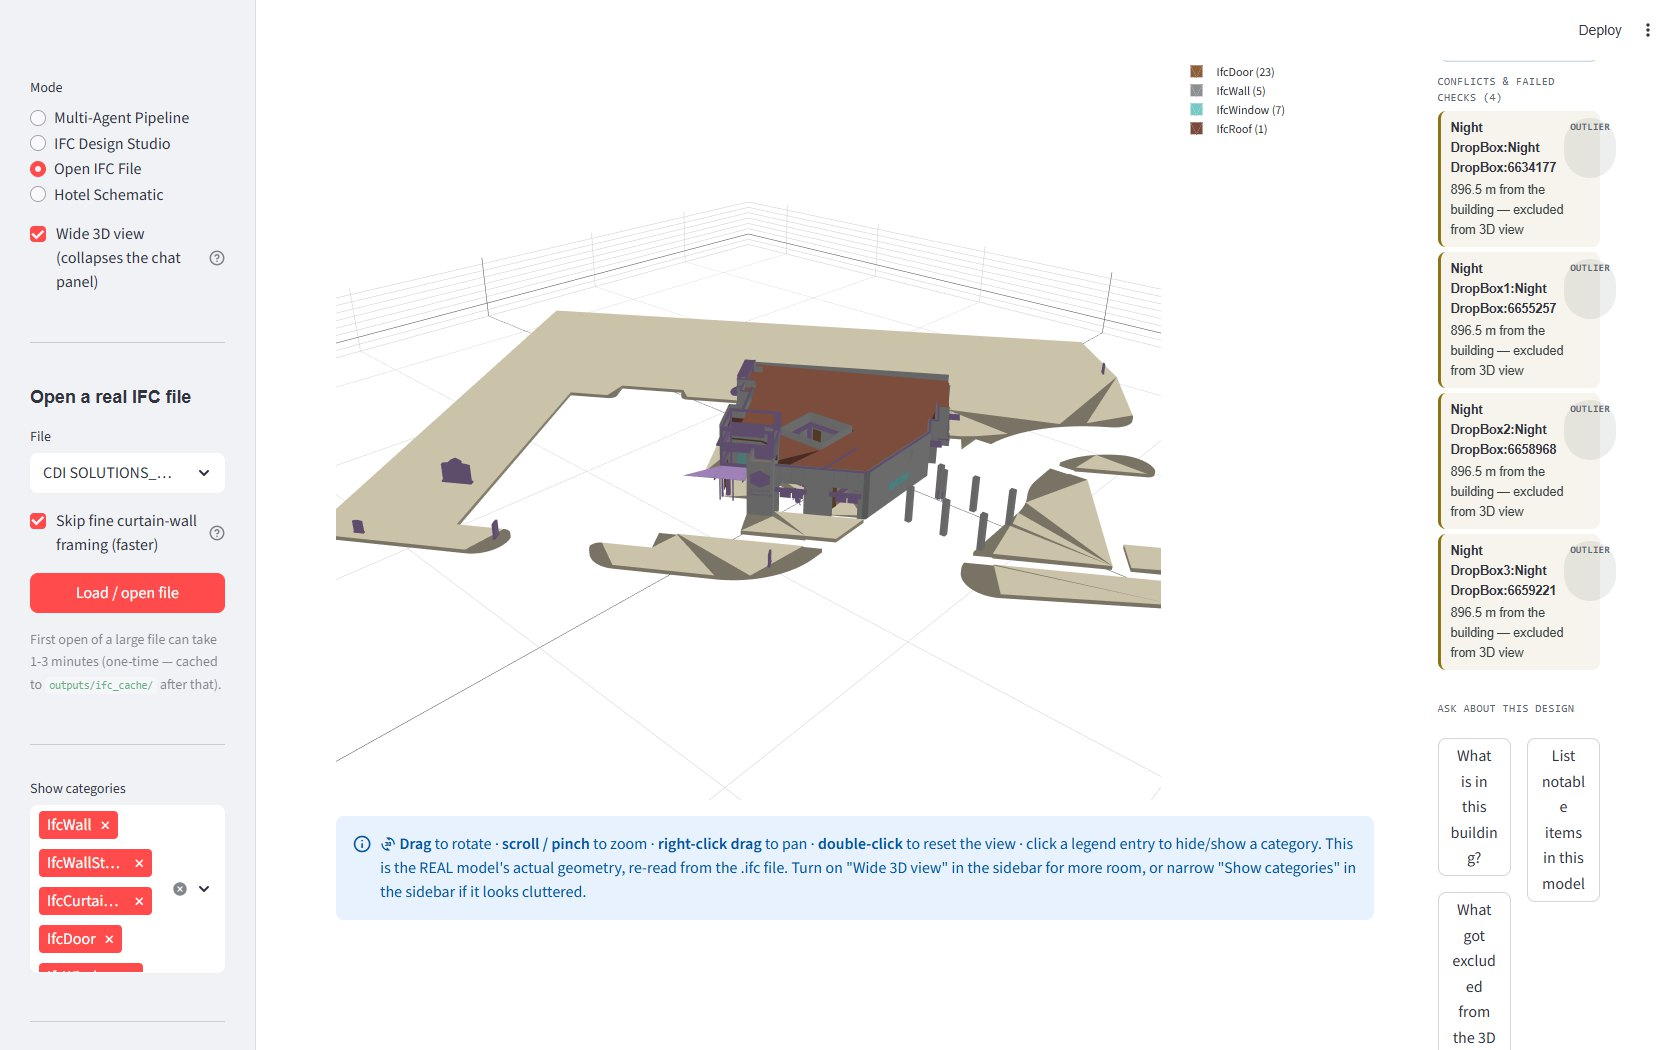
\includegraphics[width=0.92\linewidth,height=0.4\textheight,keepaspectratio]{figures/snap_17_explorer_3d_model}\caption*{\textbf{Screen 17.} A real IFC file (CDI Solutions, Metairie Bank, IFC2X3, 89 MB) recentred and shown in 3D.}\end{figure}
\begin{figure}[H]\centering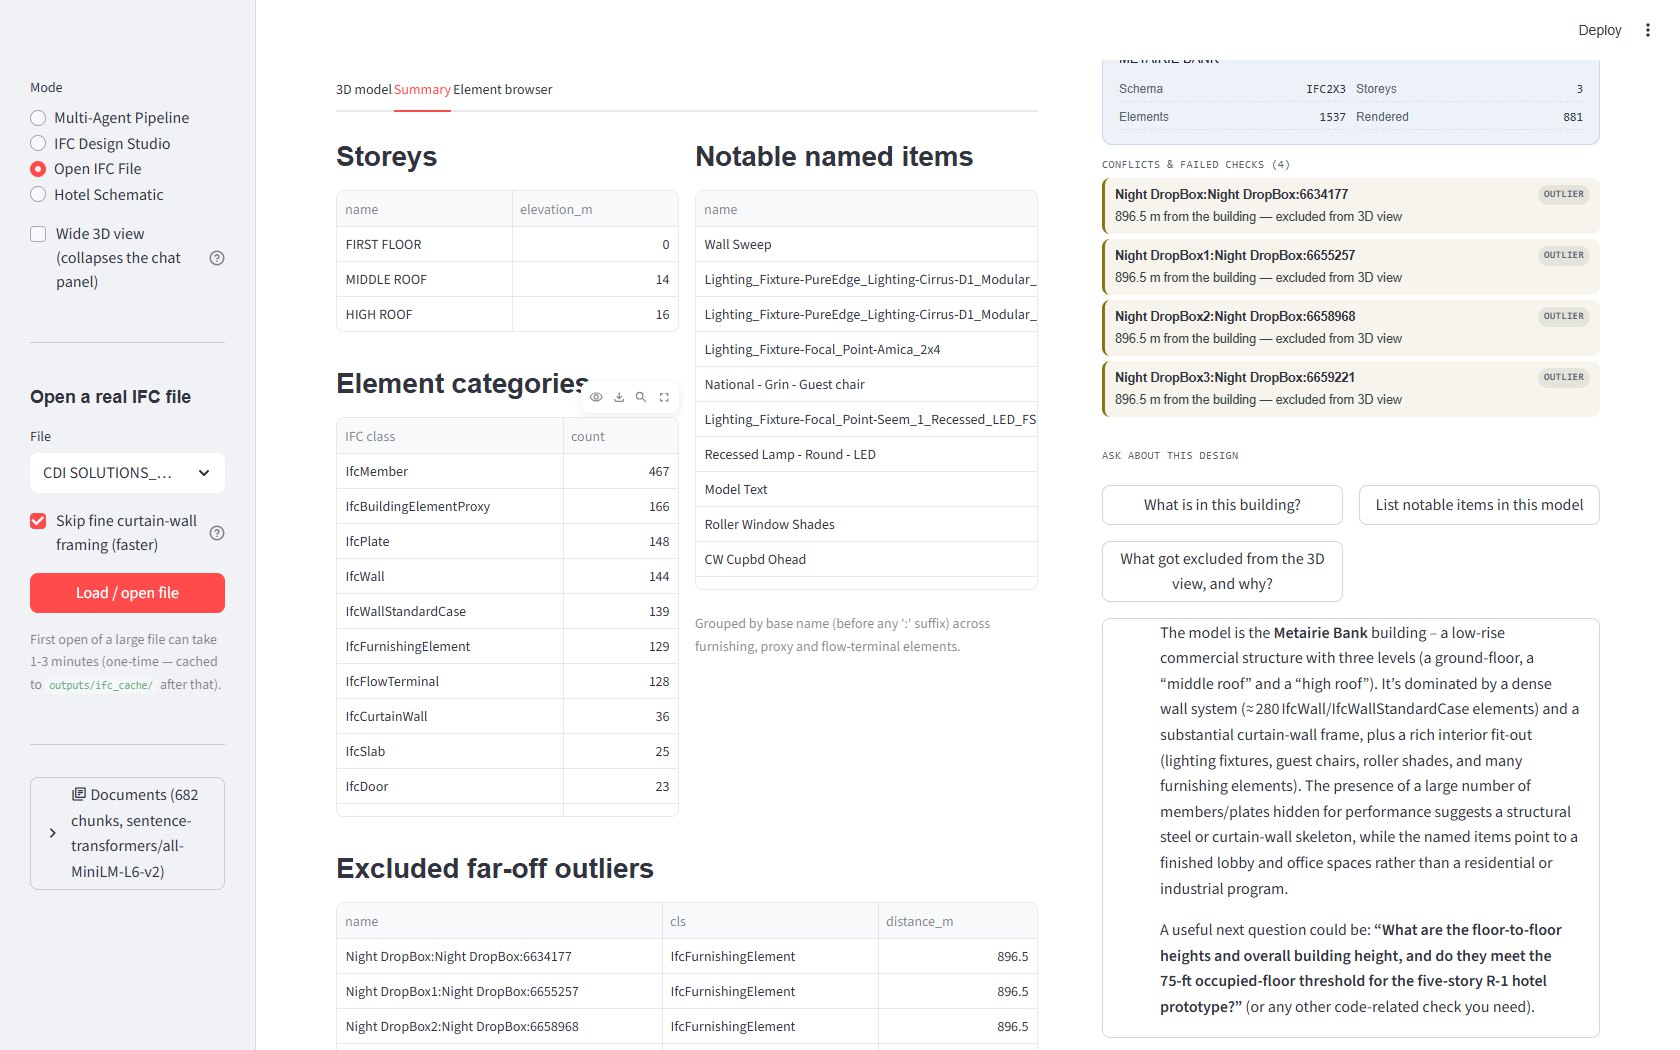
\includegraphics[width=0.92\linewidth,height=0.4\textheight,keepaspectratio]{figures/snap_18_explorer_summary}\caption*{\textbf{Screen 18.} What is in the real model: schema, storeys and element counts by IFC class.}\end{figure}
\begin{figure}[H]\centering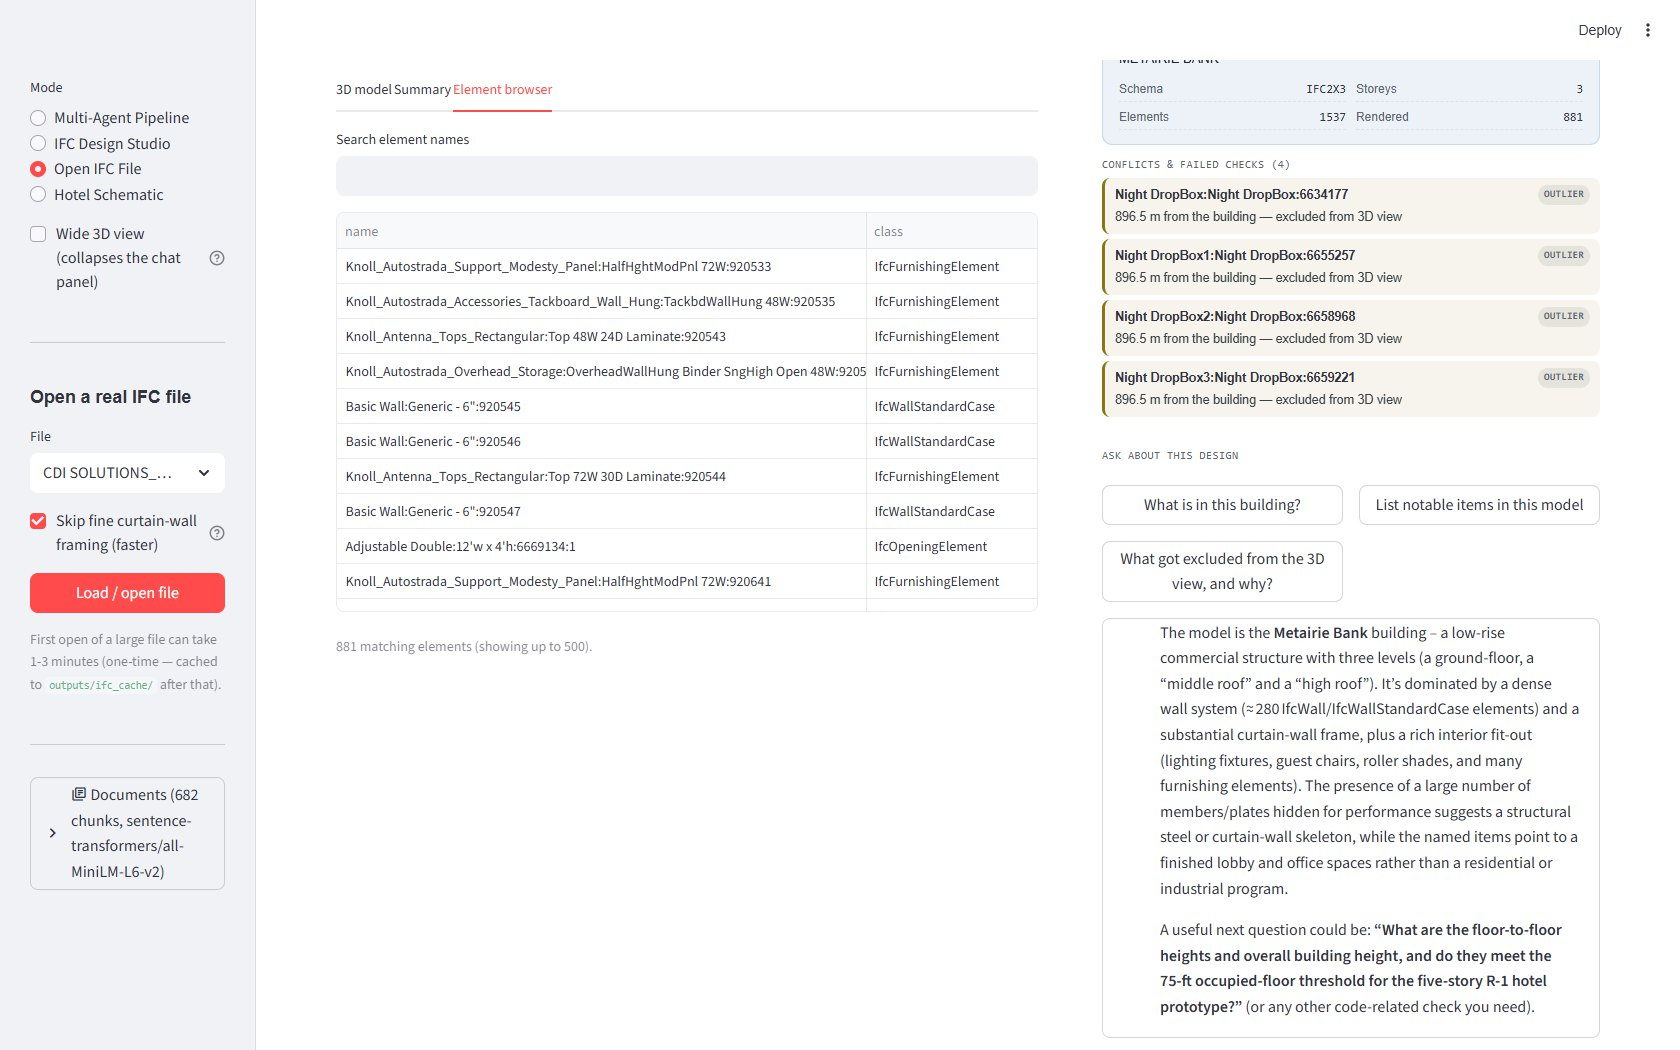
\includegraphics[width=0.92\linewidth,height=0.4\textheight,keepaspectratio]{figures/snap_19_explorer_element_browser}\caption*{\textbf{Screen 19.} Searchable list of the model's elements.}\end{figure}
\subsection*{Hotel Schematic}
\begin{figure}[H]\centering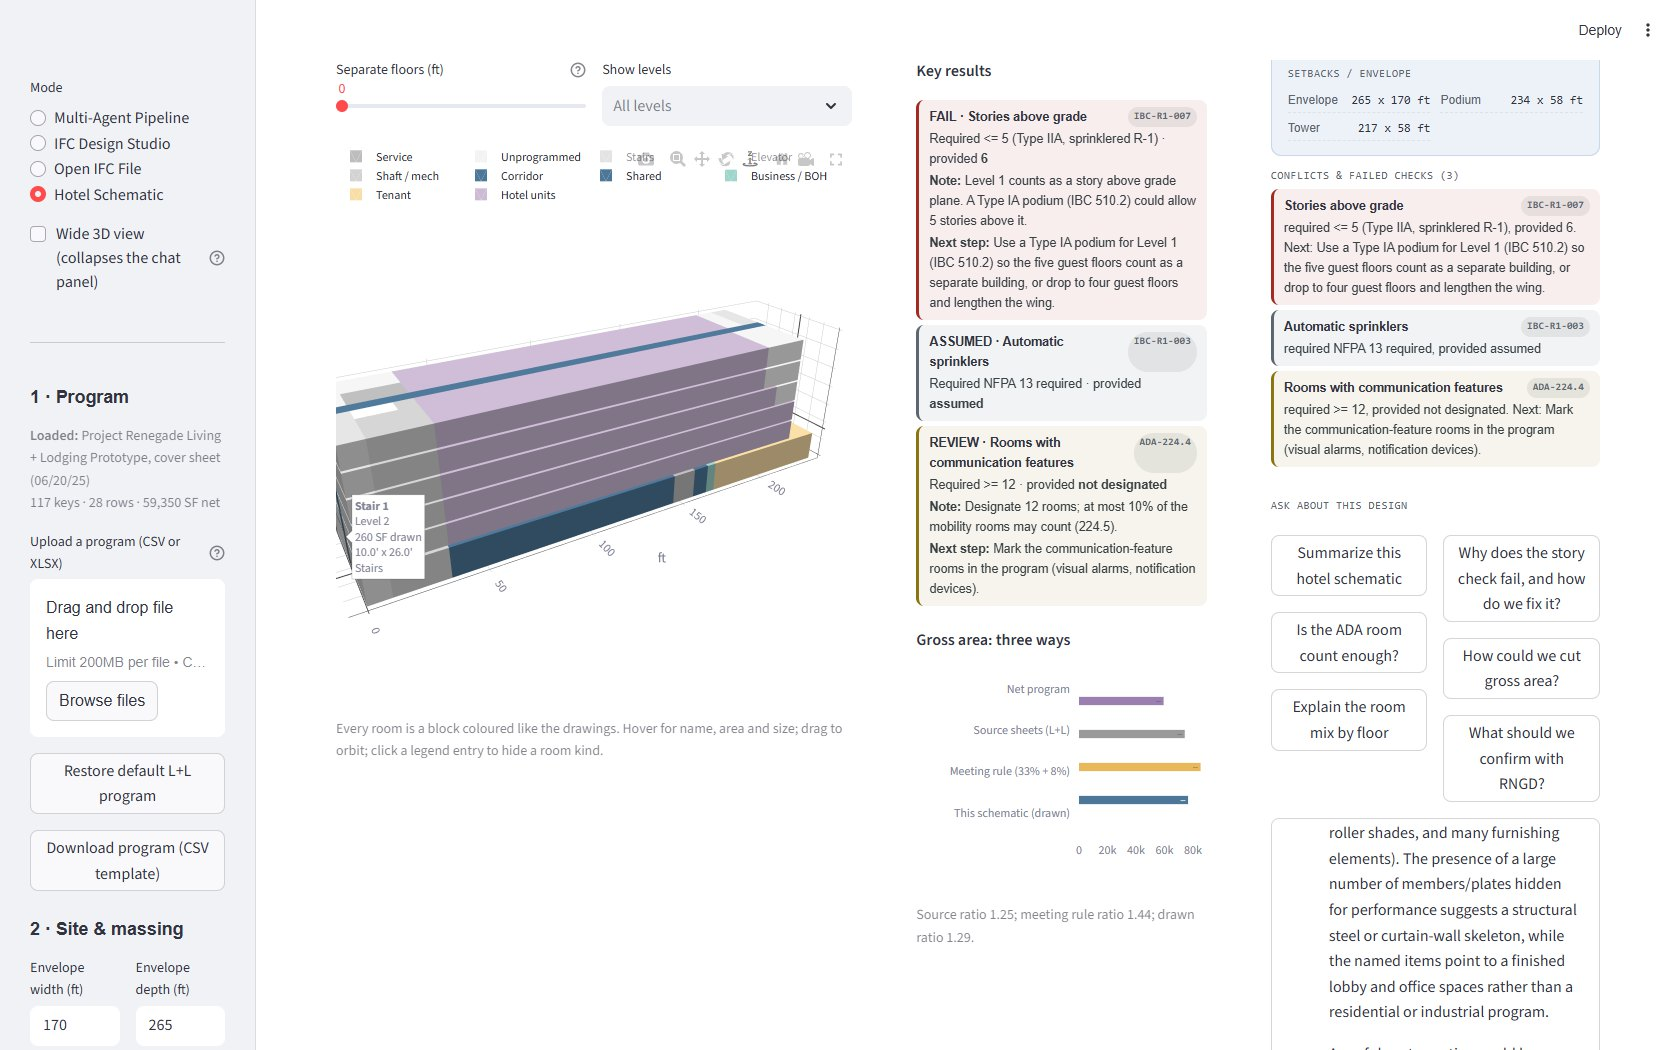
\includegraphics[width=0.92\linewidth,height=0.4\textheight,keepaspectratio]{figures/snap_20_hotel_overview}\caption*{\textbf{Screen 20.} Hotel Schematic workspace: KPI tiles, the room-by-room 3D model and the key results with suggested fixes.}\end{figure}
\begin{figure}[H]\centering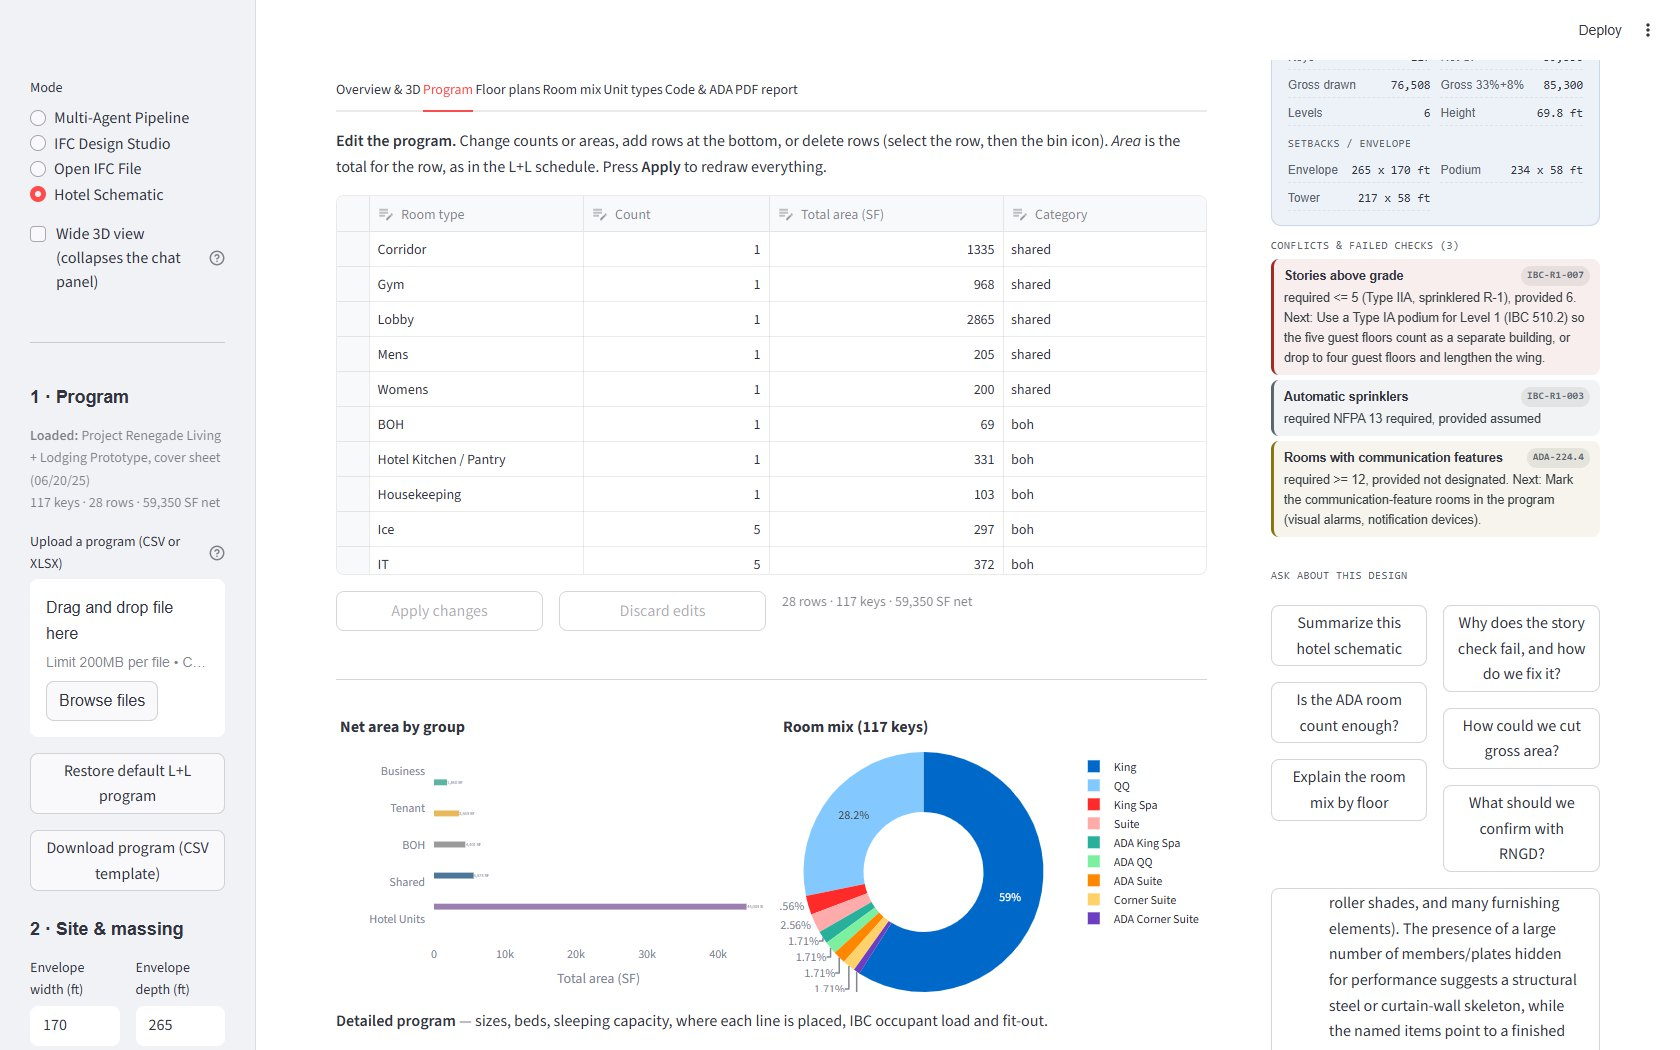
\includegraphics[width=0.92\linewidth,height=0.4\textheight,keepaspectratio]{figures/snap_21_hotel_program}\caption*{\textbf{Screen 21.} The editable program (Project Renegade L+L space allocation, 28 rows) with area and room-mix charts.}\end{figure}
\begin{figure}[H]\centering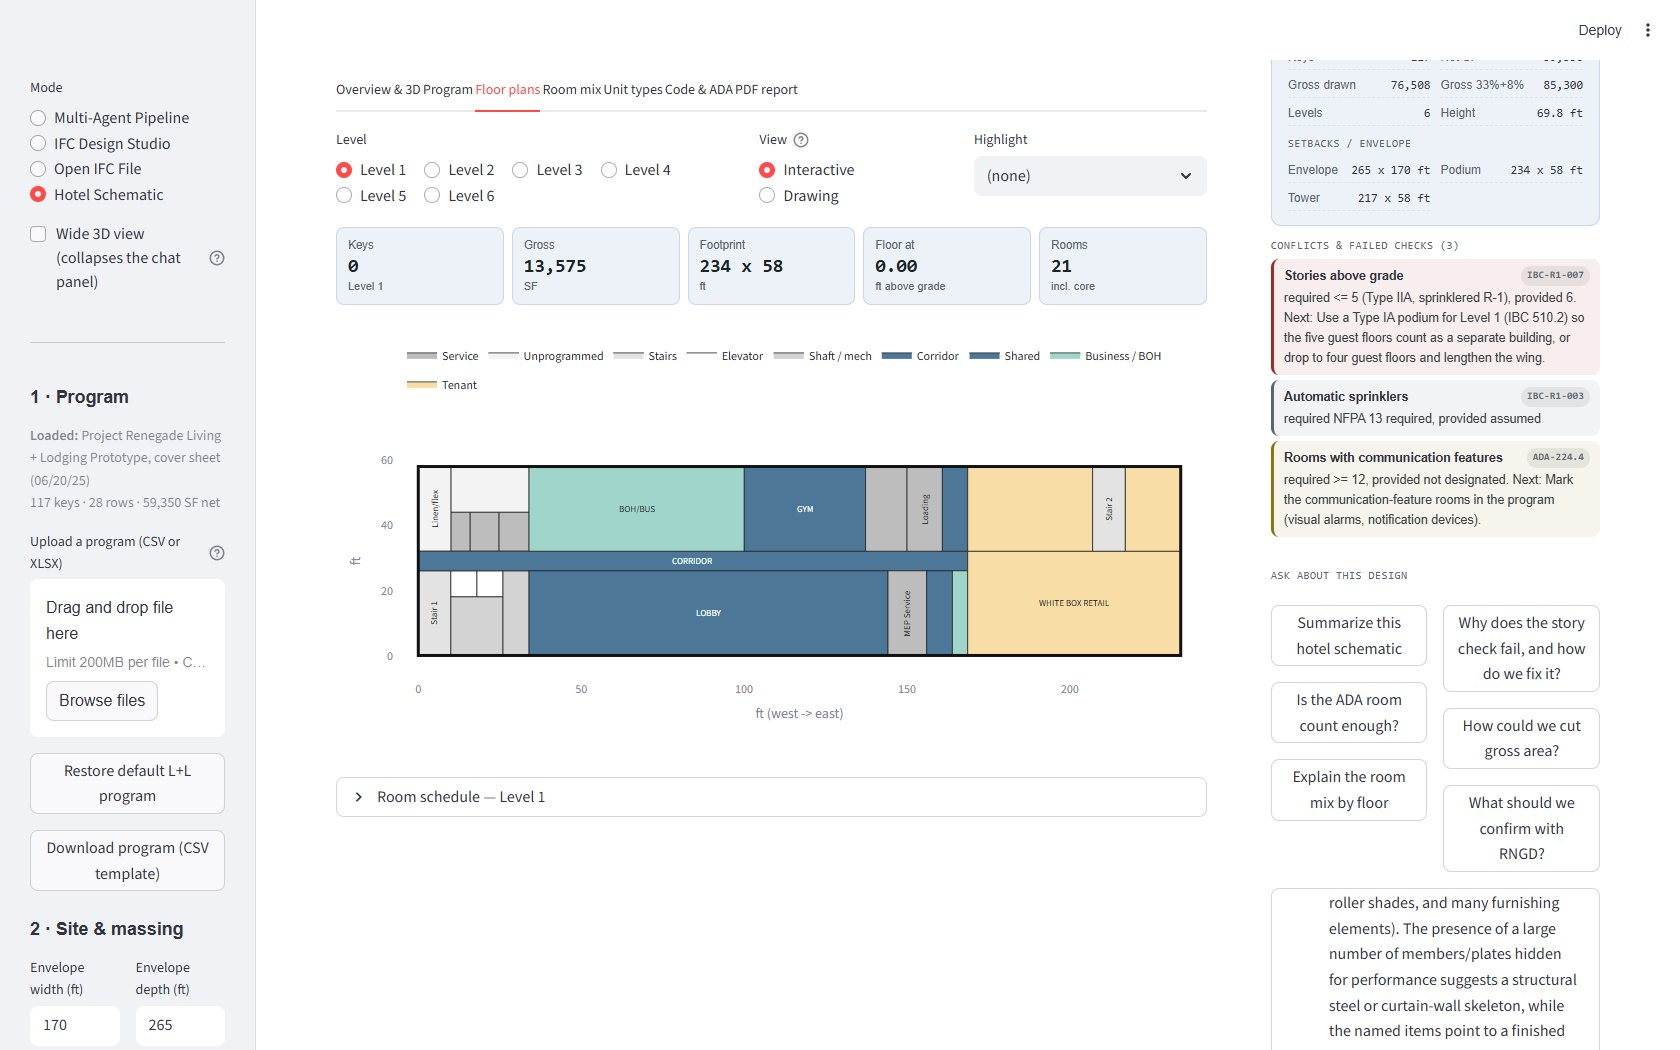
\includegraphics[width=0.92\linewidth,height=0.4\textheight,keepaspectratio]{figures/snap_22_hotel_floor}\caption*{\textbf{Screen 22.} Interactive floor plan of Level 1 (hover shows each room's area and size).}\end{figure}
\begin{figure}[H]\centering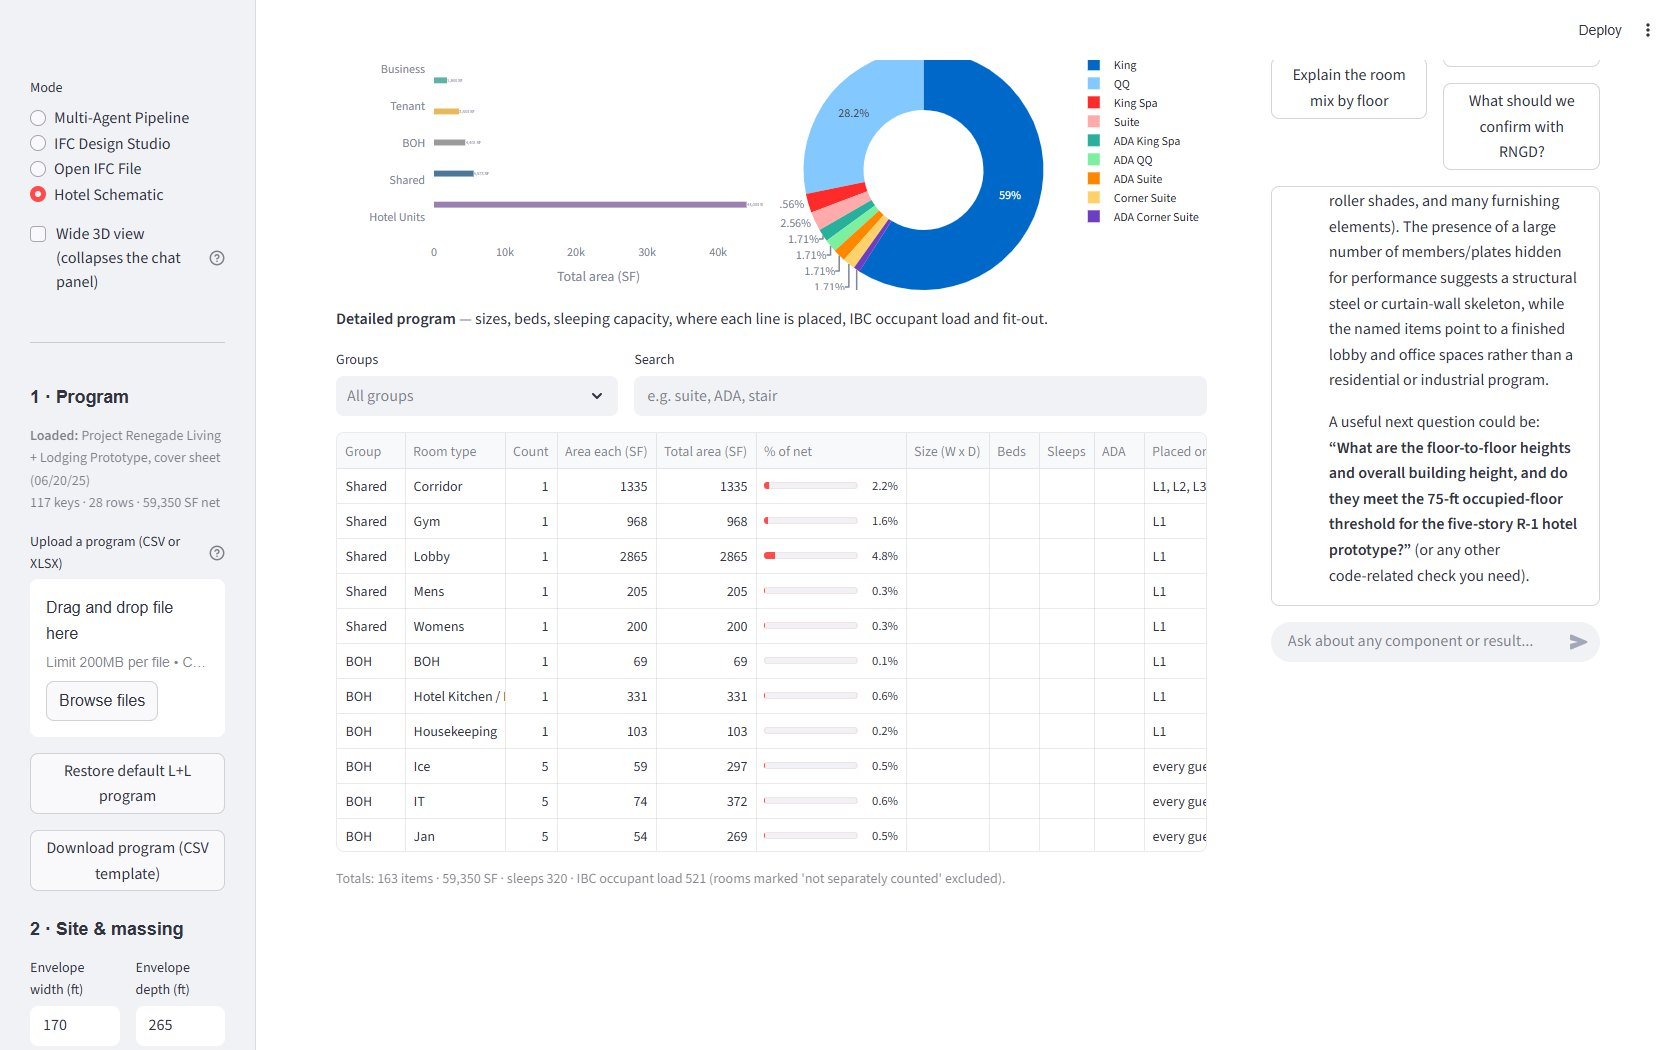
\includegraphics[width=0.92\linewidth,height=0.4\textheight,keepaspectratio]{figures/snap_23_hotel_program_detail}\caption*{\textbf{Screen 23.} Detailed program: per-room size, beds, sleeping capacity, placement, IBC occupant load and fit-out.}\end{figure}
\begin{figure}[H]\centering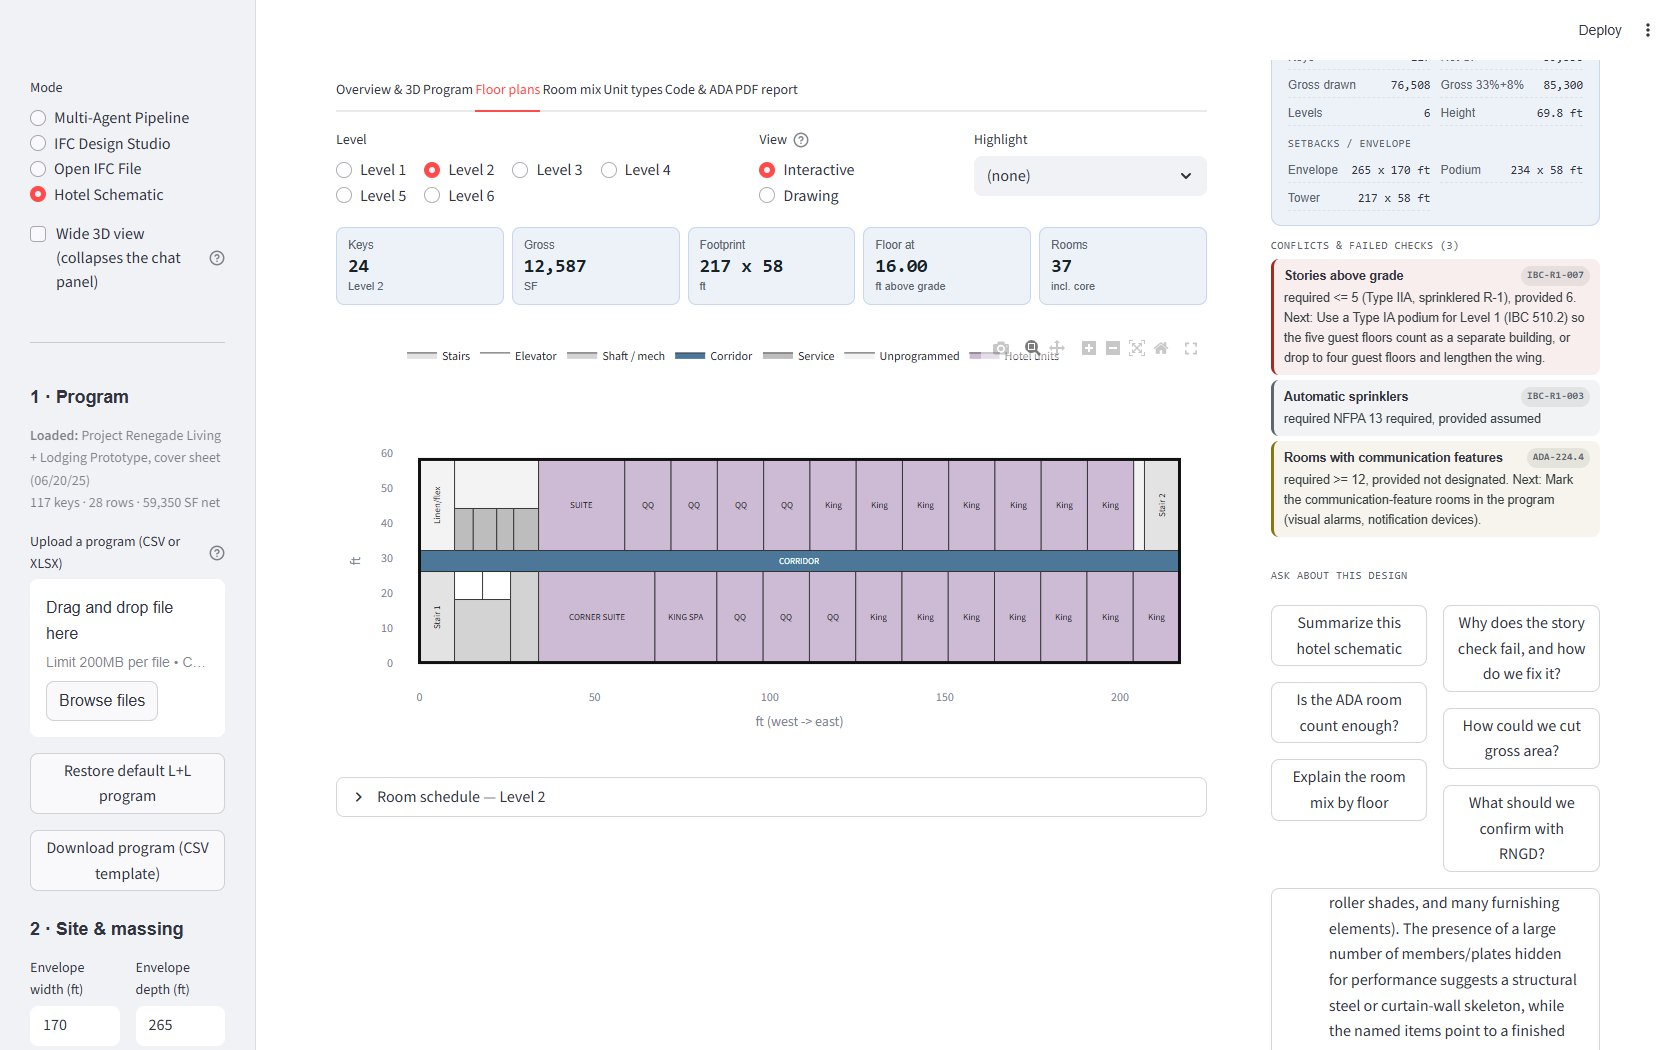
\includegraphics[width=0.92\linewidth,height=0.4\textheight,keepaspectratio]{figures/snap_24_hotel_plan_level2}\caption*{\textbf{Screen 24.} Interactive plan of Level 2, a typical guest floor (24 keys).}\end{figure}
\begin{figure}[H]\centering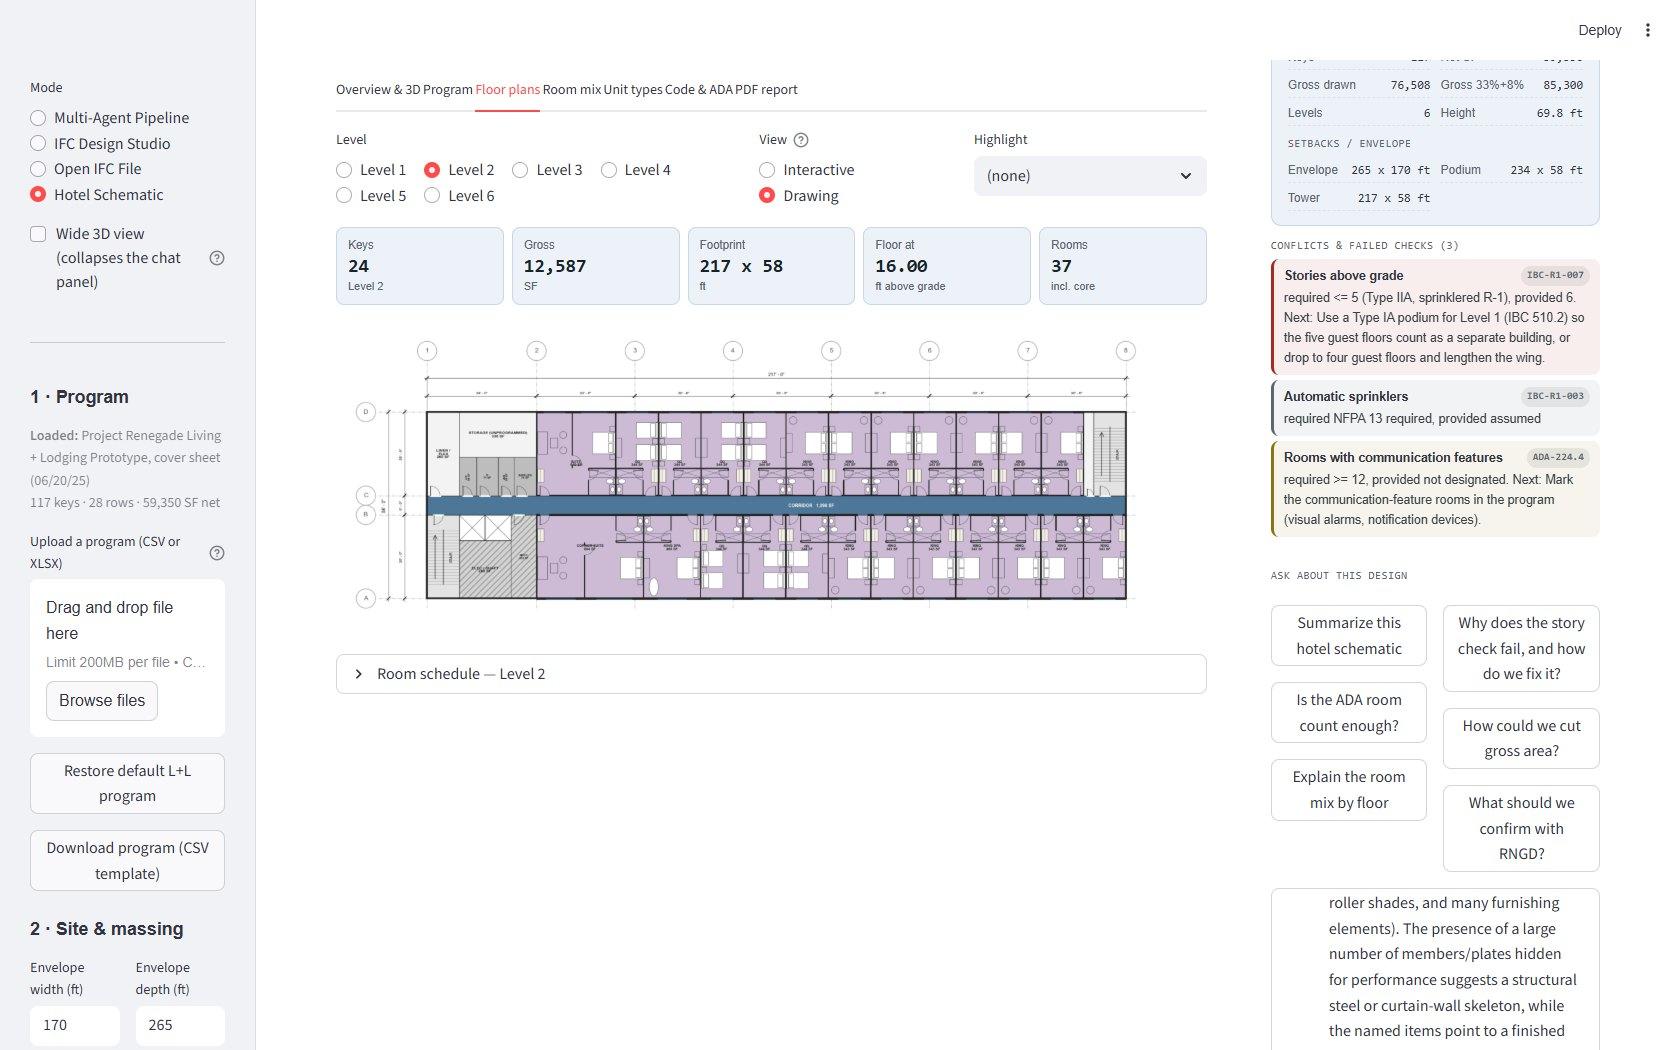
\includegraphics[width=0.92\linewidth,height=0.4\textheight,keepaspectratio]{figures/snap_25_hotel_plan_drawing}\caption*{\textbf{Screen 25.} The same level in drawing style (as used on the PDF sheets).}\end{figure}
\begin{figure}[H]\centering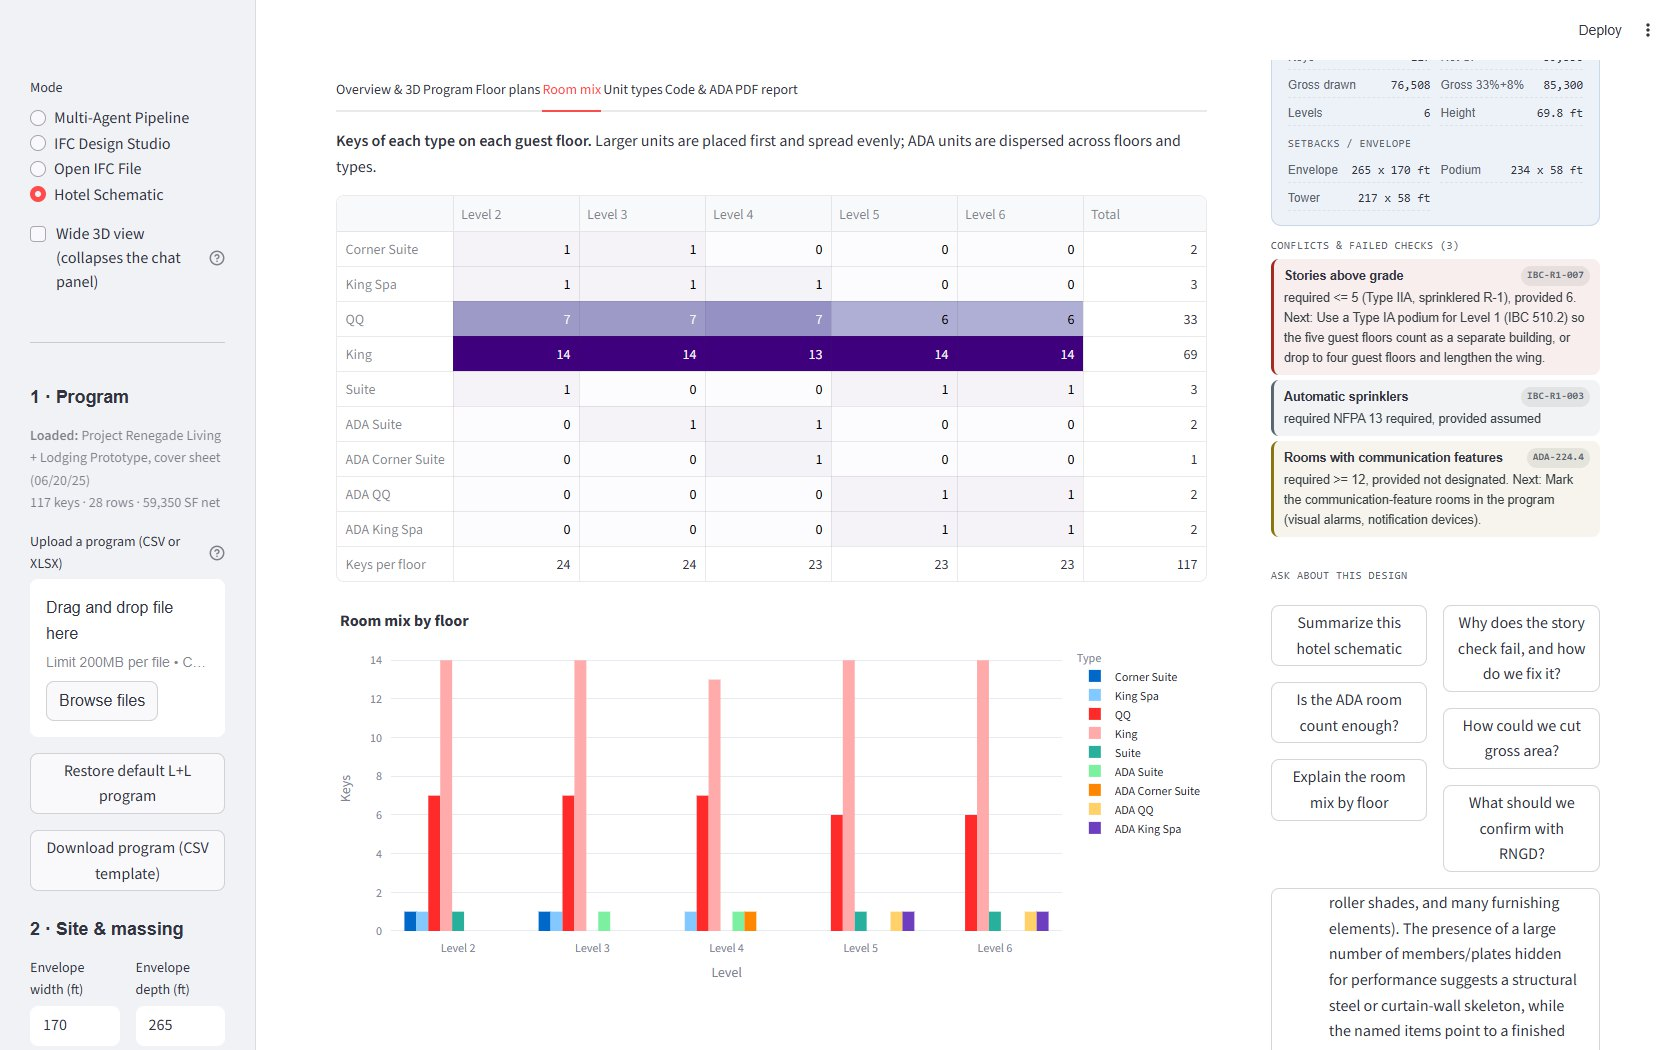
\includegraphics[width=0.92\linewidth,height=0.4\textheight,keepaspectratio]{figures/snap_26_hotel_room}\caption*{\textbf{Screen 26.} Keys of each room type on each guest floor.}\end{figure}
\begin{figure}[H]\centering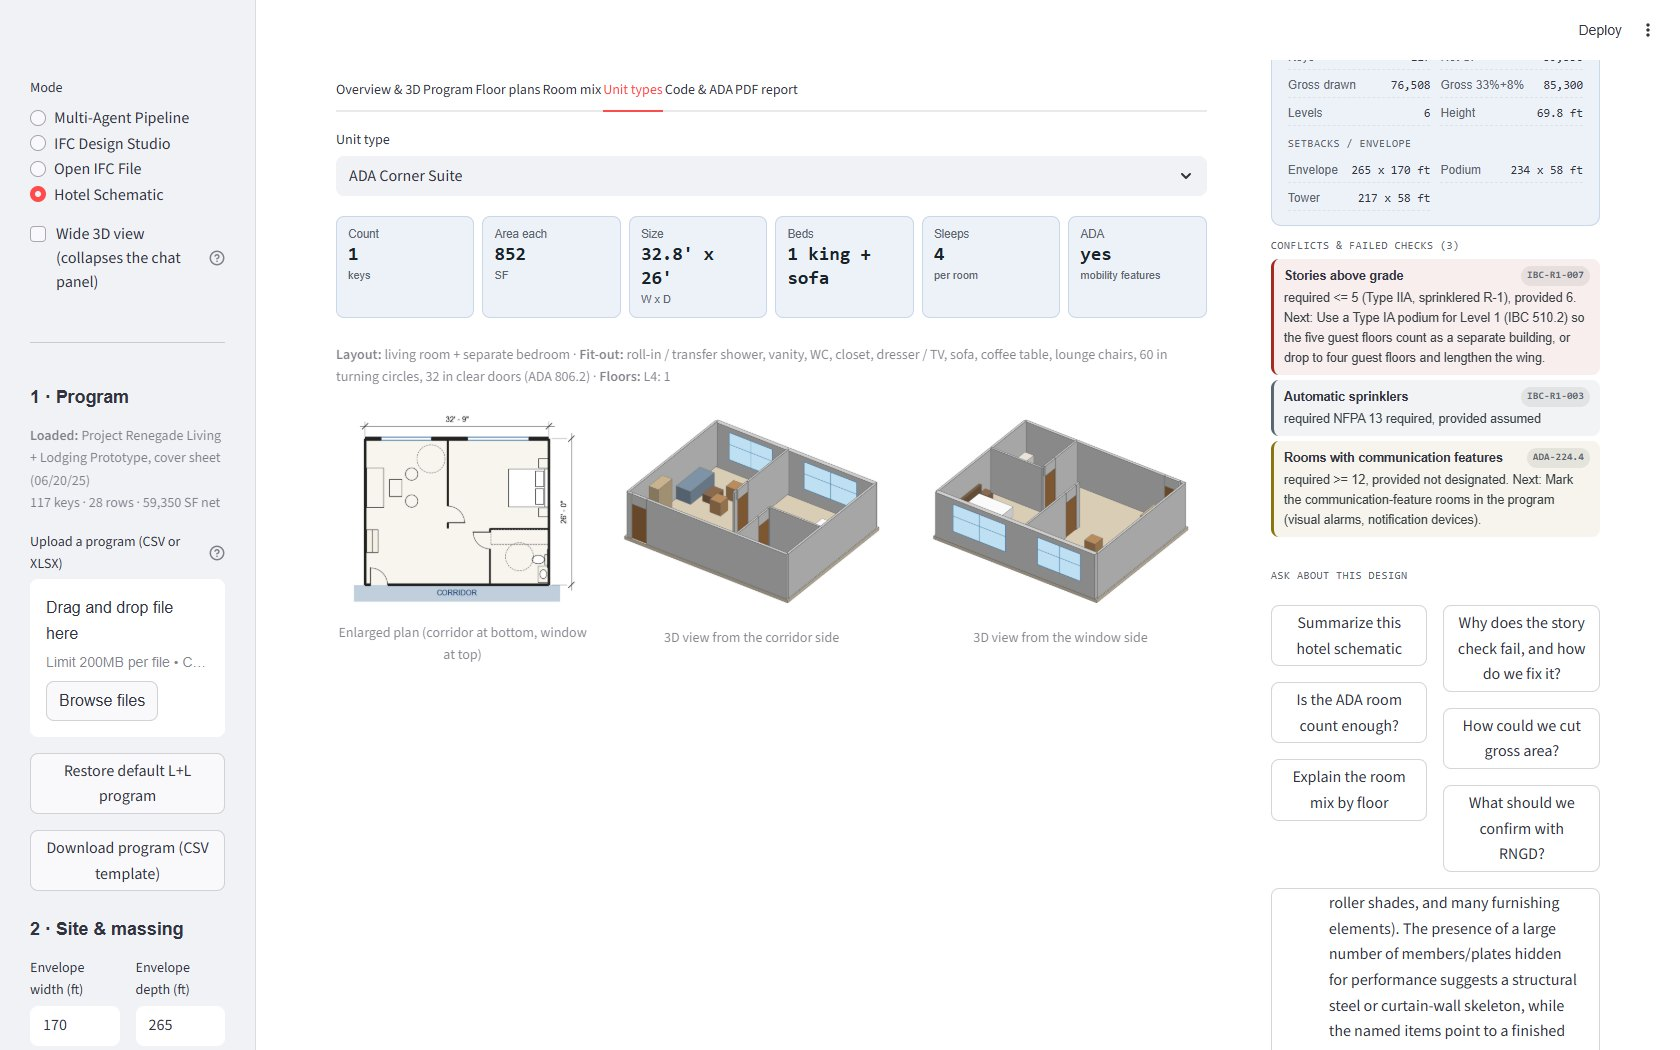
\includegraphics[width=0.92\linewidth,height=0.4\textheight,keepaspectratio]{figures/snap_27_hotel_unit}\caption*{\textbf{Screen 27.} Unit type detail: enlarged plan and two 3D interior views.}\end{figure}
\begin{figure}[H]\centering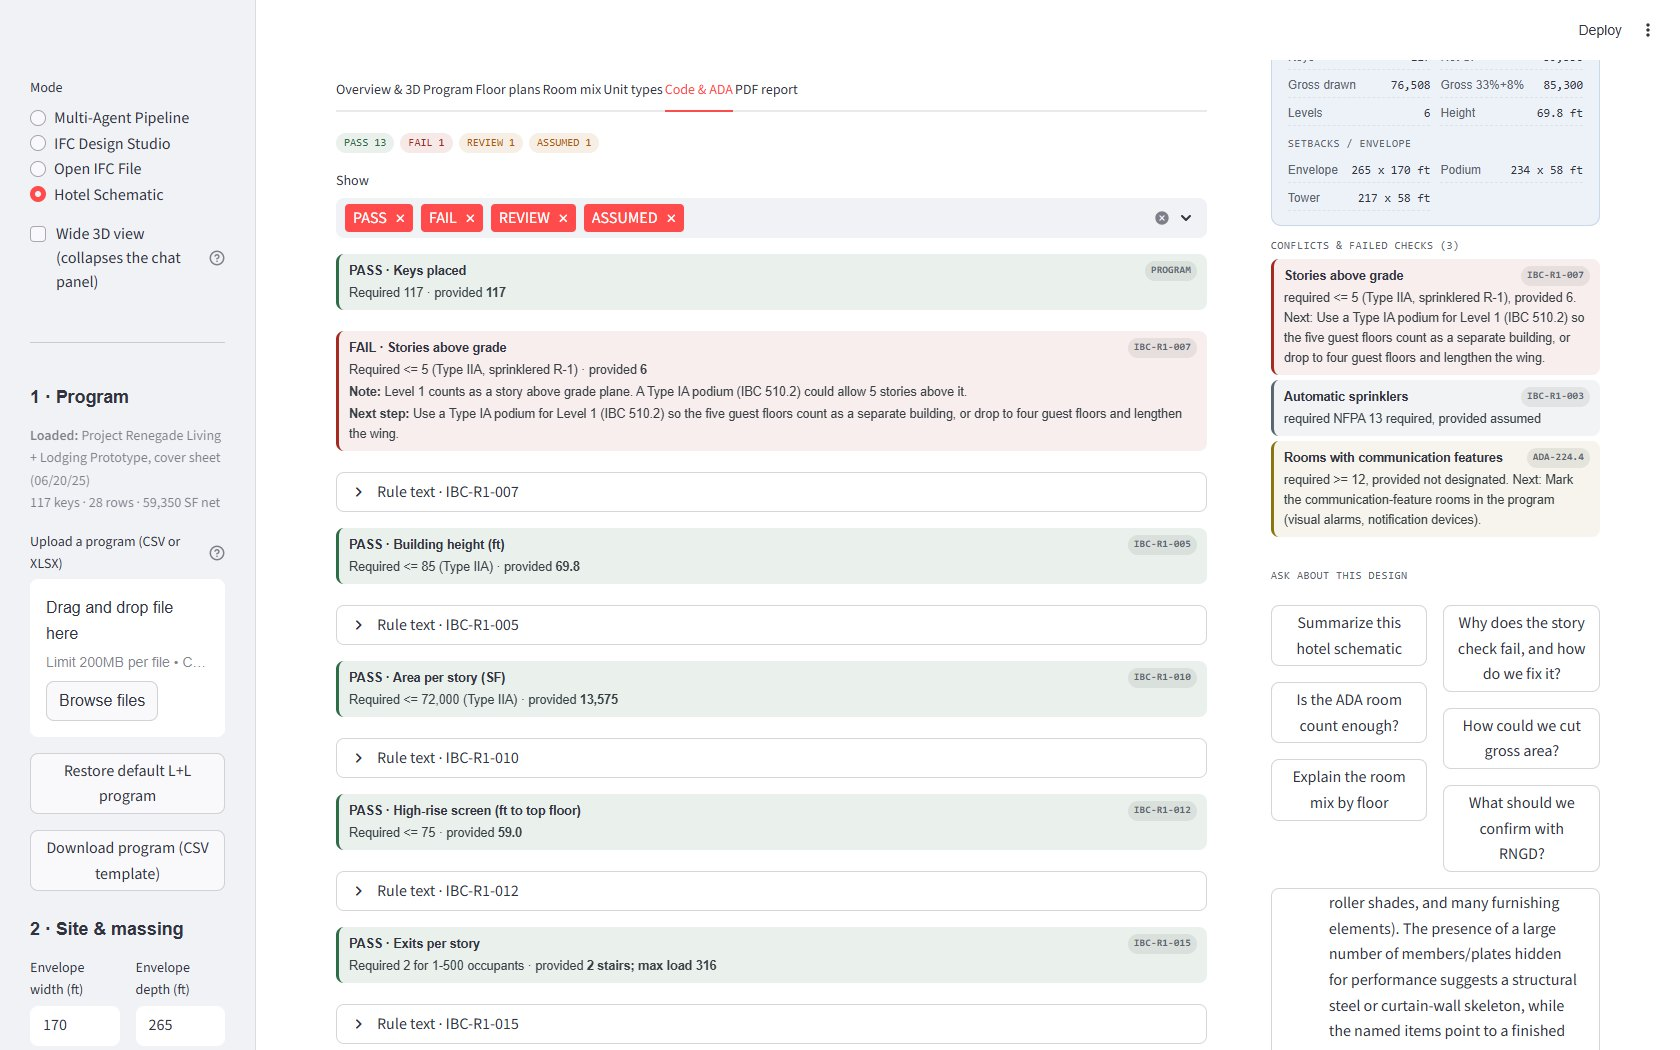
\includegraphics[width=0.92\linewidth,height=0.4\textheight,keepaspectratio]{figures/snap_28_hotel_code}\caption*{\textbf{Screen 28.} Code screen against RNGD's IBC rule set and the 2010 ADA guest-room tables, with rule text.}\end{figure}
\begin{figure}[H]\centering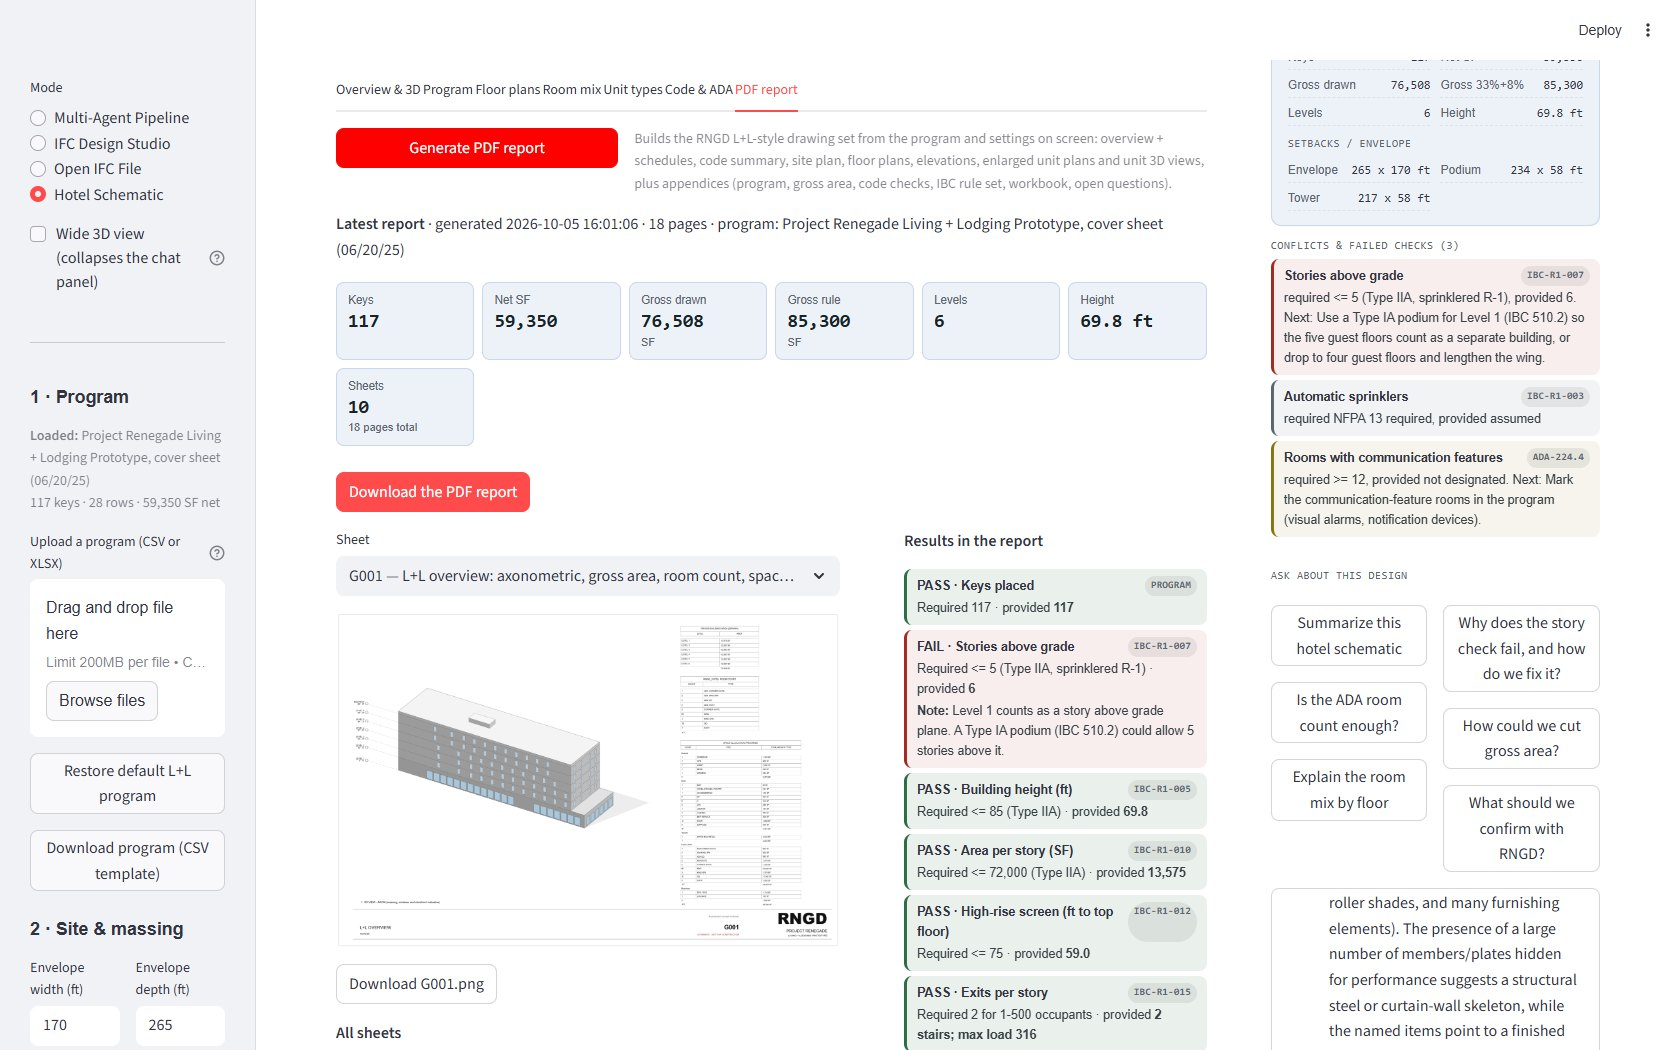
\includegraphics[width=0.92\linewidth,height=0.4\textheight,keepaspectratio]{figures/snap_29_hotel_report_results}\caption*{\textbf{Screen 29.} PDF report tab after generating: summary numbers and the results that went into the report.}\end{figure}
\begin{figure}[H]\centering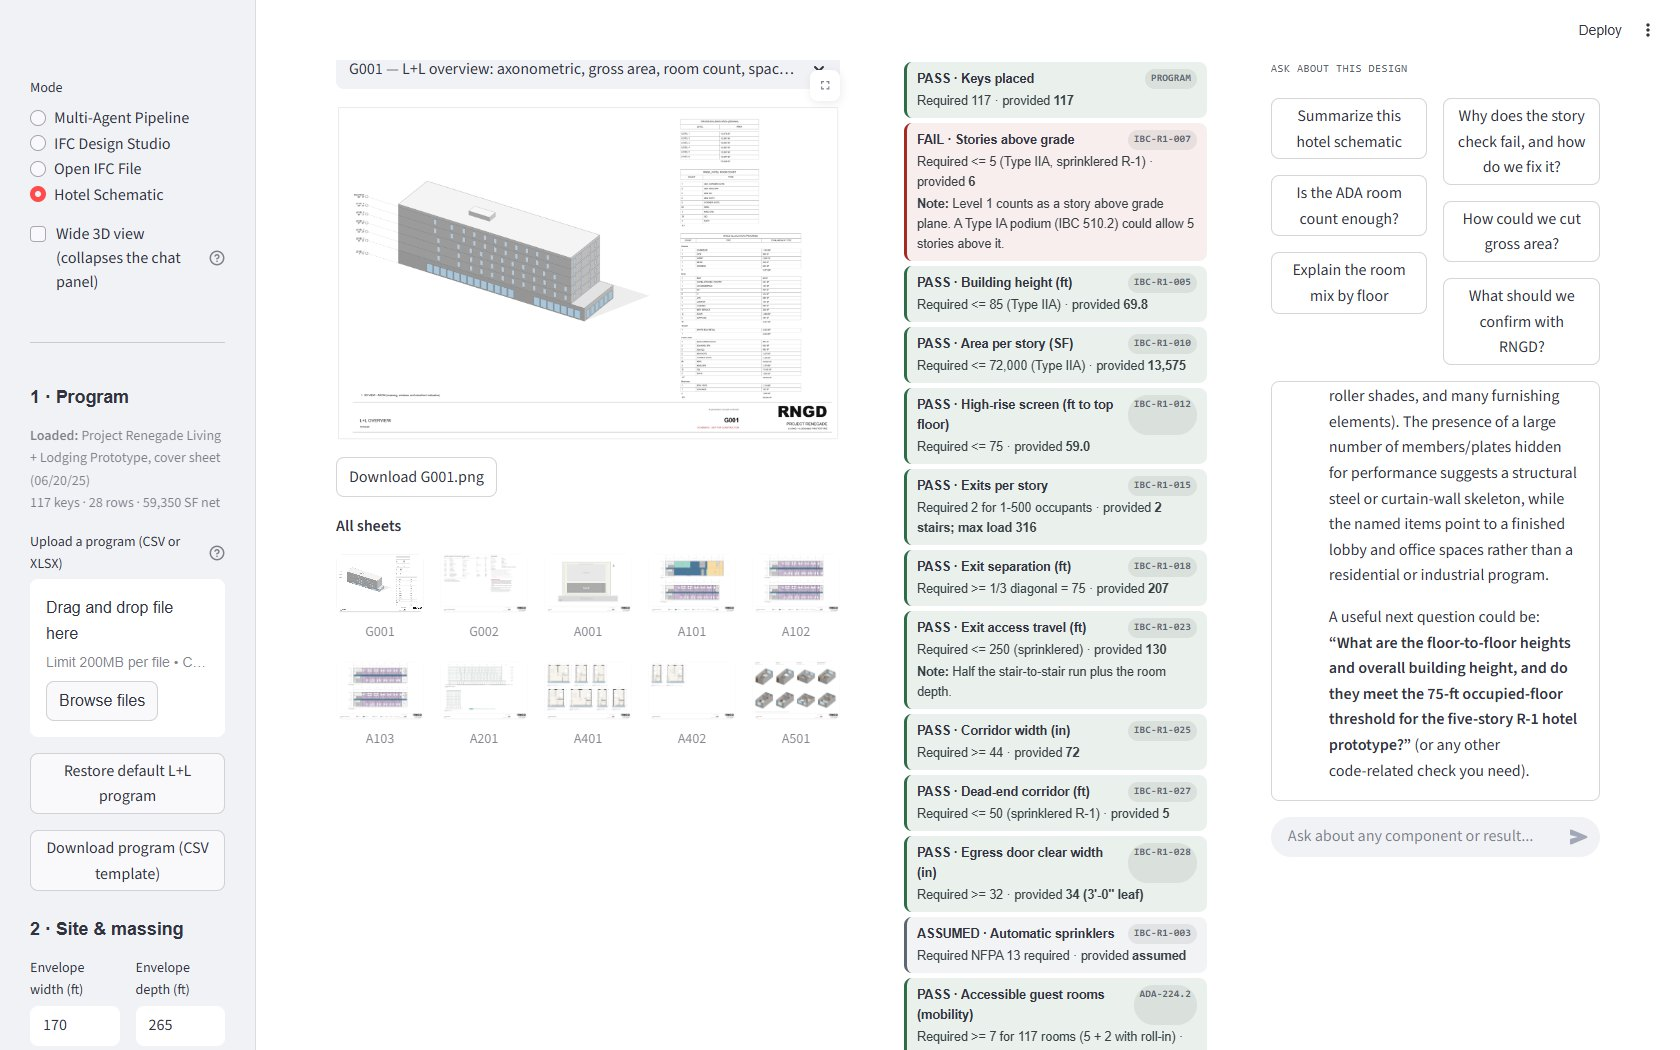
\includegraphics[width=0.92\linewidth,height=0.4\textheight,keepaspectratio]{figures/snap_30_hotel_report_sheets}\caption*{\textbf{Screen 30.} Sheet gallery of the generated drawing set.}\end{figure}
\subsection*{Assistant}
\begin{figure}[H]\centering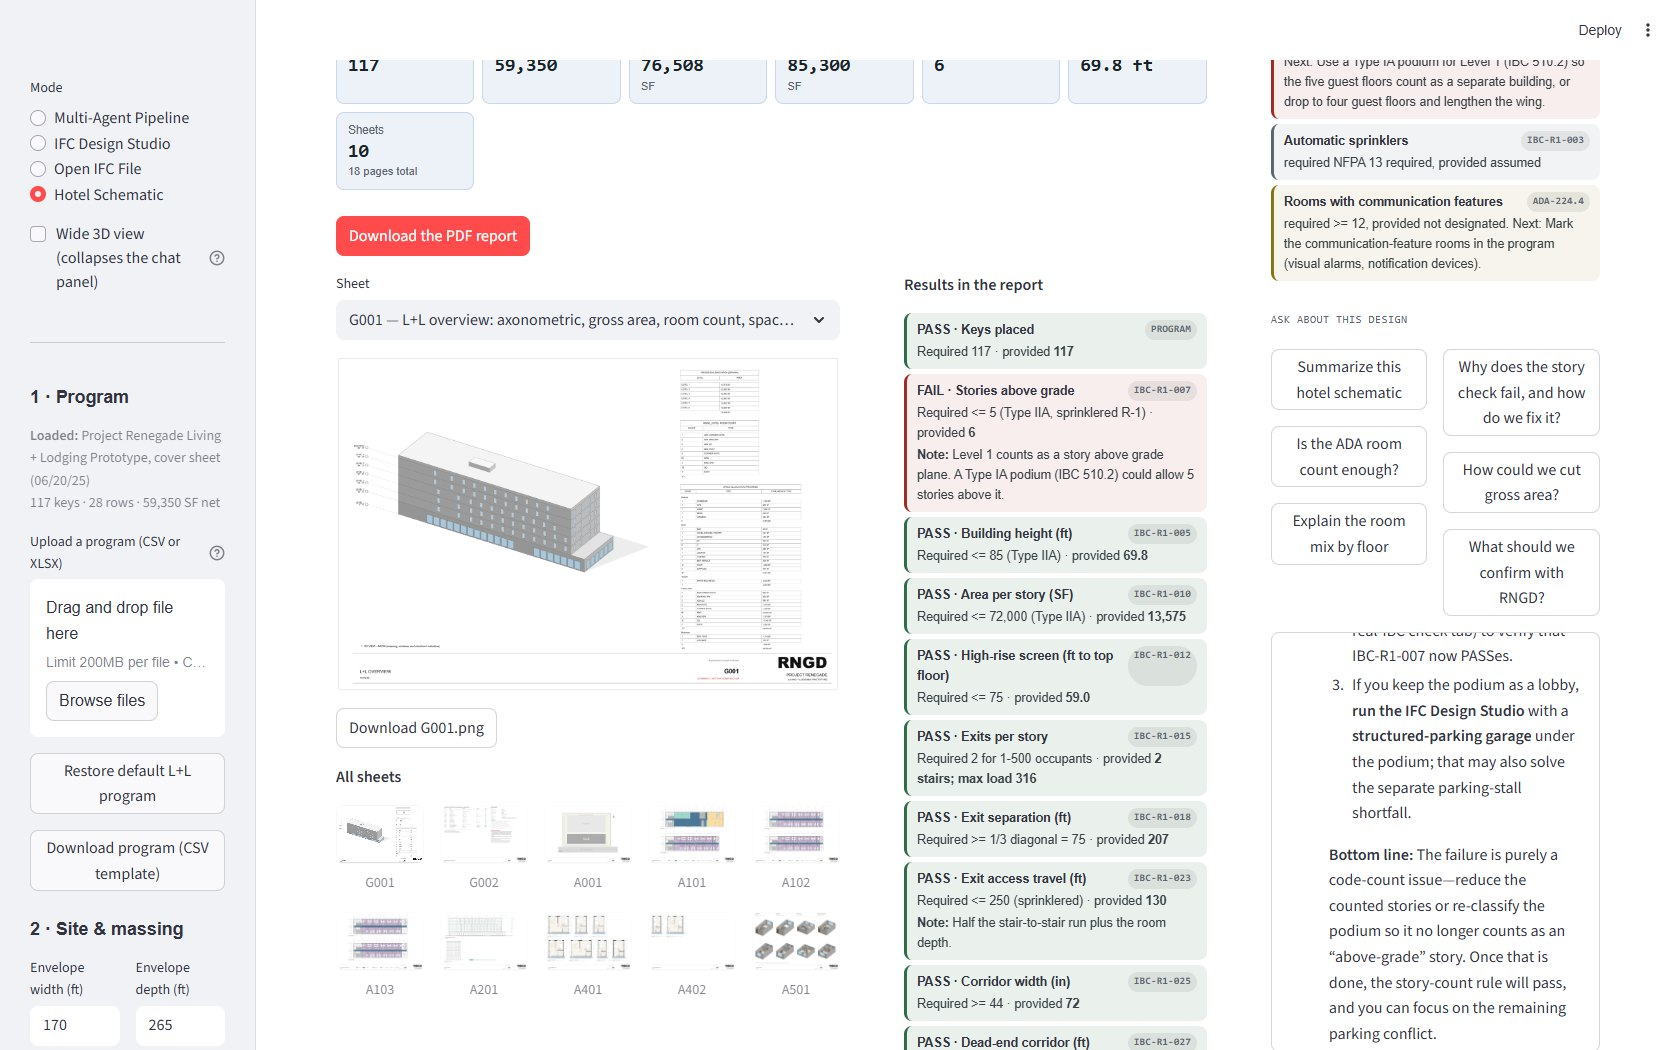
\includegraphics[width=0.92\linewidth,height=0.4\textheight,keepaspectratio]{figures/snap_31_assistant_answer}\caption*{\textbf{Screen 31.} The assistant answering a one-click question about the hotel design, using the live design state.}\end{figure}


\clearpage
\section{Reproducibility}
\label{app:repro}
\begin{lstlisting}[language=bash,numbers=none]
streamlit run src/app.py                           # the app (four modes)
python src/run_pipeline.py                         # one pipeline run
python src/build_final_report.py                   # hotel drawing set + report PDF
python src/how_it_works_experiments.py             # experiments in Section 11
python src/capture_app.py                          # browser run + screenshots
python src/run_optimizer.py --method systematic    # one optimizer run on a QA site (--method ga for the GA)
python src/build_optimizer_study.py                # optimizer comparison study (about 12 minutes)
python src/build_paper.py --no-figures             # this paper (optimizer section, code listings, PDF, Overleaf zip)
python -m pytest tests                             # 51 tests
\end{lstlisting}

\begin{table}[H]
\centering\small
\caption{Where the code lives.}
\begin{tabular}{@{}l l@{}}
\toprule
\code{src/rngd/orchestrator.py} & pipeline order, loop, floor plates \\
\code{src/rngd/agents/*.py} & the six LLM agents \\
\code{src/rngd/vectorstore.py}, \code{real\_docs.py} & knowledge base and retrieval \\
\code{src/rngd/simulation/physics\_engine.py} & physics engine \\
\code{src/rngd/vision/layout\_qa.py} & vision QA \\
\code{src/rngd/ifc/} & IFC studio, real-IFC viewer, IBC cross-check \\
\code{src/rngd/hotel/} & hotel program, layout, code screen, drawings, details, interactive views \\
\code{src/rngd/optimize/} & optimizer: plates, decoder, fitness, search, decision, views \\
\code{src/app.py}, \code{src/hotel\_ui.py} & the app \\
\code{src/hotel\_opt\_ui.py}, \code{src/optimizer\_ui.py} & the two optimizer screens \\
\bottomrule
\end{tabular}
\end{table}

\end{document}
